\documentclass{article}
\usepackage[utf8]{inputenc}
\usepackage{pgfplots}
\DeclareUnicodeCharacter{2212}{−}
\usepgfplotslibrary{groupplots,dateplot}
\usetikzlibrary{patterns,shapes.arrows}
\pgfplotsset{compat=newest}

\begin{document}

\begin{figure}
    \begin{center}
    \scalebox{0.75}{% This file was created with tikzplotlib v0.9.12.
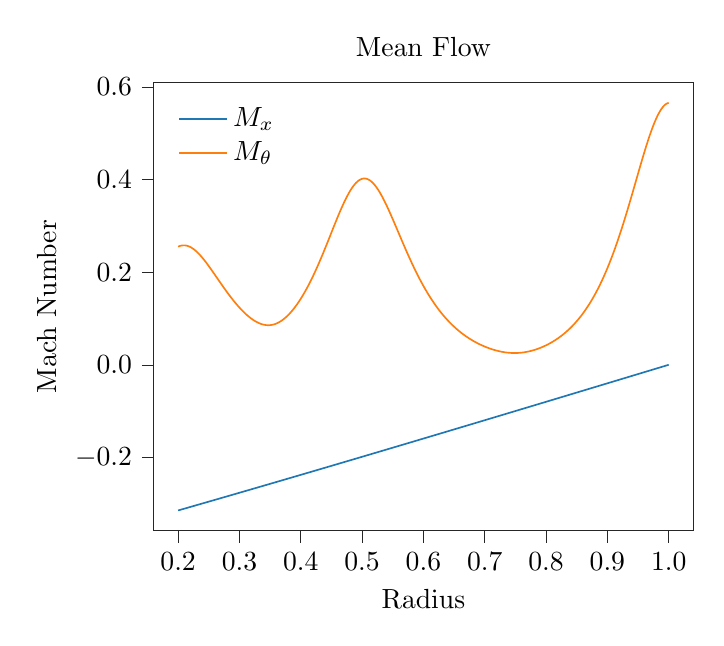
\begin{tikzpicture}

\definecolor{color0}{rgb}{0.12156862745098,0.466666666666667,0.705882352941177}
\definecolor{color1}{rgb}{1,0.498039215686275,0.0549019607843137}

\begin{axis}[
axis line style={white!15!black},
legend cell align={left},
legend style={
  fill opacity=0.8,
  draw opacity=1,
  text opacity=1,
  at={(0.03,0.97)},
  anchor=north west,
  draw=none
},
tick align=outside,
tick pos=left,
title={Mean Flow },
x grid style={white!80!black},
xlabel={Radius},
xmin=0.16, xmax=1.04,
xtick style={color=white!15!black},
xtick={0.1,0.2,0.3,0.4,0.5,0.6,0.7,0.8,0.9,1,1.1},
xticklabels={0.1,0.2,0.3,0.4,0.5,0.6,0.7,0.8,0.9,1.0,1.1},
y grid style={white!80!black},
ylabel={Mach Number},
ymin=-0.358579171685103, ymax=0.609698172253824,
ytick style={color=white!15!black},
ytick={-0.4,-0.2,0,0.2,0.4,0.6,0.8},
yticklabels={\ensuremath{-}0.4,\ensuremath{-}0.2,0.0,0.2,0.4,0.6,0.8}
]
\addplot [semithick, color0]
table {%
0.2 -0.314566565142425
0.2015625 -0.313973231598063
0.203125 -0.313379775407908
0.2046875 -0.312786196803778
0.20625 -0.31219249601754
0.2078125 -0.311598673281109
0.209375 -0.311004728826447
0.2109375 -0.310410662885563
0.2125 -0.309816475690513
0.2140625 -0.309222167473404
0.215625 -0.308627738466385
0.2171875 -0.308033188901657
0.21875 -0.307438519011464
0.2203125 -0.306843729028101
0.221875 -0.306248819183906
0.2234375 -0.305653789711266
0.225 -0.305058640842615
0.2265625 -0.304463372810433
0.228125 -0.303867985847246
0.2296875 -0.303272480185627
0.23125 -0.302676856058197
0.2328125 -0.302081113697619
0.234375 -0.301485253336607
0.2359375 -0.300889275207918
0.2375 -0.300293179544357
0.2390625 -0.299696966578772
0.240625 -0.29910063654406
0.2421875 -0.298504189673163
0.24375 -0.297907626199066
0.2453125 -0.297310946354804
0.246875 -0.296714150373453
0.2484375 -0.296117238488138
0.25 -0.295520210932026
0.2515625 -0.294923067938333
0.253125 -0.294325809740317
0.2546875 -0.293728436571281
0.25625 -0.293130948664575
0.2578125 -0.292533346253593
0.259375 -0.291935629571772
0.2609375 -0.291337798852597
0.2625 -0.290739854329594
0.2640625 -0.290141796236336
0.265625 -0.289543624806439
0.2671875 -0.288945340273564
0.26875 -0.288346942871416
0.2703125 -0.287748432833744
0.271875 -0.28714981039434
0.2734375 -0.286551075787042
0.275 -0.28595222924573
0.2765625 -0.285353271004329
0.278125 -0.284754201296807
0.2796875 -0.284155020357175
0.28125 -0.283555728419489
0.2828125 -0.282956325717846
0.284375 -0.282356812486389
0.2859375 -0.281757188959303
0.2875 -0.281157455370815
0.2890625 -0.280557611955196
0.290625 -0.27995765894676
0.2921875 -0.279357596579864
0.29375 -0.278757425088908
0.2953125 -0.278157144708332
0.296875 -0.277556755672622
0.2984375 -0.276956258216305
0.3 -0.27635565257395
0.3015625 -0.275754938980168
0.303125 -0.275154117669613
0.3046875 -0.274553188876981
0.30625 -0.273952152837011
0.3078125 -0.273351009784481
0.309375 -0.272749759954213
0.3109375 -0.27214840358107
0.3125 -0.271546940899957
0.3140625 -0.270945372145821
0.315625 -0.27034369755365
0.3171875 -0.269741917358471
0.31875 -0.269140031795357
0.3203125 -0.268538041099418
0.321875 -0.267935945505807
0.3234375 -0.267333745249717
0.325 -0.266731440566383
0.3265625 -0.266129031691081
0.328125 -0.265526518859126
0.3296875 -0.264923902305875
0.33125 -0.264321182266725
0.3328125 -0.263718358977114
0.334375 -0.263115432672518
0.3359375 -0.262512403588457
0.3375 -0.261909271960489
0.3390625 -0.261306038024212
0.340625 -0.260702702015264
0.3421875 -0.260099264169323
0.34375 -0.259495724722107
0.3453125 -0.258892083909374
0.346875 -0.258288341966921
0.3484375 -0.257684499130585
0.35 -0.257080555636242
0.3515625 -0.256476511719807
0.353125 -0.255872367617234
0.3546875 -0.255268123564519
0.35625 -0.254663779797693
0.3578125 -0.254059336552828
0.359375 -0.253454794066035
0.3609375 -0.252850152573463
0.3625 -0.252245412311301
0.3640625 -0.251640573515775
0.365625 -0.25103563642315
0.3671875 -0.25043060126973
0.36875 -0.249825468291857
0.3703125 -0.249220237725911
0.371875 -0.248614909808309
0.3734375 -0.248009484775508
0.375 -0.247403962864003
0.3765625 -0.246798344310325
0.378125 -0.246192629351044
0.3796875 -0.245586818222767
0.38125 -0.24498091116214
0.3828125 -0.244374908405845
0.384375 -0.243768810190601
0.3859375 -0.243162616753166
0.3875 -0.242556328330334
0.3890625 -0.241949945158937
0.390625 -0.241343467475843
0.3921875 -0.240736895517956
0.39375 -0.240130229522221
0.3953125 -0.239523469725615
0.396875 -0.238916616365153
0.3984375 -0.238309669677889
0.4 -0.23770262990091
0.4015625 -0.237095497271341
0.403125 -0.236488272026345
0.4046875 -0.235880954403117
0.40625 -0.235273544638891
0.4078125 -0.234666042970938
0.409375 -0.234058449636562
0.4109375 -0.233450764873104
0.4125 -0.232842988917941
0.4140625 -0.232235122008486
0.415625 -0.231627164382187
0.4171875 -0.231019116276527
0.41875 -0.230410977929025
0.4203125 -0.229802749577234
0.421875 -0.229194431458745
0.4234375 -0.228586023811182
0.425 -0.227977526872203
0.4265625 -0.227368940879503
0.428125 -0.226760266070811
0.4296875 -0.22615150268389
0.43125 -0.225542650956538
0.4328125 -0.224933711126589
0.434375 -0.224324683431909
0.4359375 -0.2237155681104
0.4375 -0.223106365399997
0.4390625 -0.222497075538671
0.440625 -0.221887698764424
0.4421875 -0.221278235315296
0.44375 -0.220668685429357
0.4453125 -0.220059049344713
0.446875 -0.219449327299504
0.4484375 -0.218839519531901
0.45 -0.21822962628011
0.4515625 -0.217619647782373
0.453125 -0.21700958427696
0.4546875 -0.21639943600218
0.45625 -0.215789203196369
0.4578125 -0.215178886097901
0.459375 -0.214568484945182
0.4609375 -0.213957999976648
0.4625 -0.21334743143077
0.4640625 -0.212736779546052
0.465625 -0.21212604456103
0.4671875 -0.211515226714272
0.46875 -0.210904326244379
0.4703125 -0.210293343389984
0.471875 -0.209682278389752
0.4734375 -0.209071131482379
0.475 -0.208459902906597
0.4765625 -0.207848592901165
0.478125 -0.207237201704876
0.4796875 -0.206625729556556
0.48125 -0.206014176695061
0.4828125 -0.205402543359278
0.484375 -0.204790829788126
0.4859375 -0.204179036220557
0.4875 -0.203567162895553
0.4890625 -0.202955210052125
0.490625 -0.202343177929319
0.4921875 -0.201731066766209
0.49375 -0.201118876801901
0.4953125 -0.200506608275533
0.496875 -0.19989426142627
0.4984375 -0.199281836493312
0.5 -0.198669333715887
0.5015625 -0.198056753333254
0.503125 -0.197444095584701
0.5046875 -0.196831360709549
0.50625 -0.196218548947147
0.5078125 -0.195605660536874
0.509375 -0.194992695718141
0.5109375 -0.194379654730386
0.5125 -0.193766537813078
0.5140625 -0.193153345205717
0.515625 -0.19254007714783
0.5171875 -0.191926733878976
0.51875 -0.191313315638742
0.5203125 -0.190699822666745
0.521875 -0.190086255202629
0.5234375 -0.18947261348607
0.525 -0.188858897756771
0.5265625 -0.188245108254466
0.528125 -0.187631245218915
0.5296875 -0.18701730888991
0.53125 -0.186403299507269
0.5328125 -0.185789217310838
0.534375 -0.185175062540495
0.5359375 -0.184560835436144
0.5375 -0.183946536237716
0.5390625 -0.183332165185173
0.540625 -0.182717722518503
0.5421875 -0.182103208477722
0.54375 -0.181488623302877
0.5453125 -0.180873967234038
0.546875 -0.180259240511305
0.5484375 -0.179644443374807
0.55 -0.179029576064698
0.5515625 -0.178414638821162
0.553125 -0.177799631884408
0.5546875 -0.177184555494672
0.55625 -0.17656940989222
0.5578125 -0.175954195317341
0.559375 -0.175338912010356
0.5609375 -0.174723560211609
0.5625 -0.17410814016147
0.5640625 -0.17349265210034
0.565625 -0.172877096268643
0.5671875 -0.17226147290683
0.56875 -0.17164578225538
0.5703125 -0.171030024554796
0.571875 -0.170414200045609
0.5734375 -0.169798308968375
0.575 -0.169182351563677
0.5765625 -0.168566328072123
0.578125 -0.167950238734347
0.5796875 -0.16733408379101
0.58125 -0.166717863482796
0.5828125 -0.166101578050417
0.584375 -0.165485227734609
0.5859375 -0.164868812776134
0.5875 -0.164252333415779
0.5890625 -0.163635789894357
0.590625 -0.163019182452705
0.5921875 -0.162402511331685
0.59375 -0.161785776772184
0.5953125 -0.161168979015113
0.596875 -0.160552118301411
0.5984375 -0.159935194872038
0.6 -0.159318208967979
0.6015625 -0.158701160830245
0.603125 -0.158084050699871
0.6046875 -0.157466878817914
0.60625 -0.156849645425458
0.6078125 -0.156232350763609
0.609375 -0.155614995073498
0.6109375 -0.154997578596281
0.6125 -0.154380101573134
0.6140625 -0.15376256424526
0.615625 -0.153144966853885
0.6171875 -0.152527309640257
0.61875 -0.151909592845649
0.6203125 -0.151291816711356
0.621875 -0.150673981478698
0.6234375 -0.150056087389016
0.625 -0.149438134683675
0.6265625 -0.148820123604062
0.628125 -0.14820205439159
0.6296875 -0.147583927287689
0.63125 -0.146965742533818
0.6328125 -0.146347500371453
0.634375 -0.145729201042096
0.6359375 -0.14511084478727
0.6375 -0.144492431848521
0.6390625 -0.143873962467415
0.640625 -0.143255436885543
0.6421875 -0.142636855344516
0.64375 -0.142018218085968
0.6453125 -0.141399525351553
0.646875 -0.140780777382949
0.6484375 -0.140161974421854
0.65 -0.139543116709988
0.6515625 -0.138924204489092
0.653125 -0.138305238000929
0.6546875 -0.137686217487282
0.65625 -0.137067143189957
0.6578125 -0.136448015350779
0.659375 -0.135828834211595
0.6609375 -0.135209600014273
0.6625 -0.134590313000702
0.6640625 -0.133970973412789
0.665625 -0.133351581492465
0.6671875 -0.13273213748168
0.66875 -0.132112641622403
0.6703125 -0.131493094156626
0.671875 -0.13087349532636
0.6734375 -0.130253845373634
0.675 -0.1296341445405
0.6765625 -0.129014393069028
0.678125 -0.12839459120131
0.6796875 -0.127774739179454
0.68125 -0.127154837245591
0.6828125 -0.12653488564187
0.684375 -0.125914884610459
0.6859375 -0.125294834393547
0.6875 -0.12467473523334
0.6890625 -0.124054587372064
0.690625 -0.123434391051966
0.6921875 -0.122814146515309
0.69375 -0.122193854004376
0.6953125 -0.121573513761469
0.696875 -0.120953126028908
0.6984375 -0.120332691049032
0.7 -0.1197122090642
0.7015625 -0.119091680316785
0.703125 -0.118471105049183
0.7046875 -0.117850483503806
0.70625 -0.117229815923084
0.7078125 -0.116609102549465
0.709375 -0.115988343625415
0.7109375 -0.115367539393419
0.7125 -0.114746690095978
0.7140625 -0.114125795975612
0.715625 -0.113504857274856
0.7171875 -0.112883874236266
0.71875 -0.112262847102412
0.7203125 -0.111641776115884
0.721875 -0.111020661519287
0.7234375 -0.110399503555244
0.725 -0.109778302466396
0.7265625 -0.109157058495398
0.728125 -0.108535771884924
0.7296875 -0.107914442877665
0.73125 -0.107293071716326
0.7328125 -0.106671658643631
0.734375 -0.10605020390232
0.7359375 -0.105428707735148
0.7375 -0.104807170384887
0.7390625 -0.104185592094326
0.740625 -0.103563973106267
0.7421875 -0.102942313663532
0.74375 -0.102320614008955
0.7453125 -0.101698874385389
0.746875 -0.1010770950357
0.7484375 -0.100455276202771
0.75 -0.0998334181294999
0.7515625 -0.0992115210587998
0.753125 -0.0985895852335994
0.7546875 -0.0979676108968424
0.75625 -0.0973455982914874
0.7578125 -0.0967235476605083
0.759375 -0.0961014592468934
0.7609375 -0.0954793332936462
0.7625 -0.0948571700437845
0.7640625 -0.0942349697403408
0.765625 -0.0936127326263622
0.7671875 -0.0929904589449099
0.76875 -0.0923681489390598
0.7703125 -0.0917458028519016
0.771875 -0.0911234209265392
0.7734375 -0.0905010034060907
0.775 -0.0898785505336877
0.7765625 -0.0892560625524761
0.778125 -0.0886335397056152
0.7796875 -0.0880109822362778
0.78125 -0.0873883903876507
0.7828125 -0.0867657644029336
0.784375 -0.0861431045253399
0.7859375 -0.0855204109980961
0.7875 -0.0848976840644419
0.7890625 -0.0842749239676299
0.790625 -0.0836521309509258
0.7921875 -0.0830293052576081
0.79375 -0.0824064471309682
0.7953125 -0.0817835568143099
0.796875 -0.0811606345509499
0.7984375 -0.0805376805842171
0.8 -0.0799146951574529
0.8015625 -0.079291678514011
0.803125 -0.0786686308972572
0.8046875 -0.0780455525505696
0.80625 -0.0774224437173381
0.8078125 -0.0767993046409646
0.809375 -0.0761761355648628
0.8109375 -0.0755529367324582
0.8125 -0.0749297083871877
0.8140625 -0.0743064507724999
0.815625 -0.0736831641318549
0.8171875 -0.073059848708724
0.81875 -0.0724365047465898
0.8203125 -0.071813132488946
0.821875 -0.0711897321792973
0.8234375 -0.0705663040611597
0.825 -0.0699428483780596
0.8265625 -0.0693193653735343
0.828125 -0.0686958552911321
0.8296875 -0.0680723183744114
0.83125 -0.0674487548669416
0.8328125 -0.0668251650123019
0.834375 -0.0662015490540821
0.8359375 -0.0655779072358824
0.8375 -0.0649542398013126
0.8390625 -0.0643305469939931
0.840625 -0.0637068290575537
0.8421875 -0.0630830862356343
0.84375 -0.0624593187718844
0.8453125 -0.0618355269099631
0.846875 -0.0612117108935392
0.8484375 -0.0605878709662909
0.85 -0.0599640073719054
0.8515625 -0.0593401203540797
0.853125 -0.0587162101565195
0.8546875 -0.0580922770229398
0.85625 -0.0574683211970645
0.8578125 -0.0568443429226261
0.859375 -0.0562203424433665
0.8609375 -0.0555963200030356
0.8625 -0.0549722758453923
0.8640625 -0.0543482102142038
0.865625 -0.0537241233532457
0.8671875 -0.0531000155063021
0.86875 -0.0524758869171648
0.8703125 -0.0518517378296344
0.871875 -0.0512275684875189
0.8734375 -0.0506033791346345
0.875 -0.0499791700148053
0.8765625 -0.0493549413718627
0.878125 -0.0487306934496463
0.8796875 -0.0481064264920028
0.88125 -0.0474821407427864
0.8828125 -0.0468578364458589
0.884375 -0.0462335138450891
0.8859375 -0.045609173184353
0.8875 -0.0449848147075337
0.8890625 -0.0443604386585211
0.890625 -0.0437360452812123
0.8921875 -0.0431116348195108
0.89375 -0.042487207517327
0.8953125 -0.0418627636185779
0.896875 -0.0412383033671867
0.8984375 -0.0406138270070833
0.9 -0.0399893347822038
0.9015625 -0.0393648269364904
0.903125 -0.0387403037138917
0.9046875 -0.0381157653583617
0.90625 -0.037491212113861
0.9078125 -0.0368666442243555
0.909375 -0.0362420619338172
0.9109375 -0.0356174654862236
0.9125 -0.0349928551255574
0.9140625 -0.0343682310958073
0.915625 -0.0337435936409669
0.9171875 -0.0331189430050354
0.91875 -0.0324942794320168
0.9203125 -0.0318696031659202
0.921875 -0.03124491445076
0.9234375 -0.0306202135305551
0.925 -0.0299955006493293
0.9265625 -0.0293707760511112
0.928125 -0.0287460399799336
0.9296875 -0.0281212926798342
0.93125 -0.0274965343948549
0.9328125 -0.0268717653690419
0.934375 -0.0262469858464456
0.9359375 -0.0256221960711204
0.9375 -0.024997396287125
0.9390625 -0.0243725867385215
0.940625 -0.0237477676693765
0.9421875 -0.0231229393237598
0.94375 -0.0224981019457448
0.9453125 -0.0218732557794089
0.946875 -0.0212484010688324
0.9484375 -0.0206235380580993
0.95 -0.0199986669912967
0.9515625 -0.0193737881125147
0.953125 -0.0187489016658469
0.9546875 -0.0181240078953893
0.95625 -0.0174991070452412
0.9578125 -0.0168741993595044
0.959375 -0.0162492850822834
0.9609375 -0.0156243644576856
0.9625 -0.0149994377298203
0.9640625 -0.0143745051427998
0.965625 -0.0137495669407382
0.9671875 -0.0131246233677519
0.96875 -0.0124996746679598
0.9703125 -0.0118747210854821
0.971875 -0.0112497628644416
0.9734375 -0.0106248002489625
0.975 -0.00999983348317079
0.9765625 -0.00937486281119418
0.978125 -0.00874988847716171
0.9796875 -0.00812491072520414
0.98125 -0.00749992979945334
0.9828125 -0.00687494594404237
0.984375 -0.00624995940310574
0.9859375 -0.00562497042077864
0.9875 -0.00499997924119756
0.9890625 -0.0043749861084996
0.990625 -0.00374999126682261
0.9921875 -0.00312499496030536
0.99375 -0.00249999743308688
0.9953125 -0.00187499892930699
0.996875 -0.00124999969310565
0.9984375 -0.000624999968623085
1 0
};
\addlegendentry{$M_{x}$}
\addplot [semithick, color1]
table {%
0.2 0.255065159843046
0.2015625 0.255968364411969
0.203125 0.256706833358219
0.2046875 0.257279572376127
0.20625 0.257686110072619
0.2078125 0.257926497257104
0.209375 0.258001302302394
0.2109375 0.257911602675627
0.2125 0.257658972790116
0.2140625 0.257245468377284
0.215625 0.256673607621338
0.2171875 0.255946349337276
0.21875 0.255067068504603
0.2203125 0.254039529494257
0.221875 0.25286785734447
0.2234375 0.251556507452602
0.225 0.250110234054432
0.2265625 0.248534057860345
0.228125 0.246833233209701
0.2296875 0.245013215091013
0.23125 0.243079626357068
0.2328125 0.241038225441498
0.234375 0.238894874857357
0.2359375 0.236655510729794
0.2375 0.234326113584628
0.2390625 0.231912680583411
0.240625 0.229421199363994
0.2421875 0.226857623614387
0.24375 0.224227850477382
0.2453125 0.221537699854474
0.246875 0.218792895650435
0.2484375 0.21599904897482
0.25 0.21316164329395
0.2515625 0.210286021506594
0.253125 0.207377374898871
0.2546875 0.204440733918698
0.25625 0.201480960697466
0.2578125 0.198502743236421
0.259375 0.19551059116732
0.2609375 0.192508832991191
0.2625 0.189501614695225
0.2640625 0.186492899645885
0.265625 0.183486469655856
0.2671875 0.180485927123467
0.26875 0.177494698145321
0.2703125 0.174516036506022
0.271875 0.171553028452757
0.2734375 0.168608598167034
0.275 0.165685513850817
0.2765625 0.162786394349561
0.278125 0.159913716240034
0.2796875 0.157069821316225
0.28125 0.154256924411978
0.2828125 0.151477121504055
0.284375 0.148732398044197
0.2859375 0.146024637473106
0.2875 0.143355629873271
0.2890625 0.140727080720902
0.290625 0.138140619700031
0.2921875 0.13559780954393
0.29375 0.133100154870287
0.2953125 0.130649110977115
0.296875 0.128246092566015
0.2984375 0.125892482358112
0.3 0.123589639565741
0.3015625 0.121338908179735
0.303125 0.119141625027891
0.3046875 0.116999127554962
0.30625 0.114912761268305
0.3078125 0.112883886786253
0.309375 0.110913886418458
0.3109375 0.109004170199123
0.3125 0.107156181285485
0.3140625 0.105371400625434
0.315625 0.103651350790409
0.3171875 0.1019975988631
0.31875 0.100411758264908
0.3203125 0.0988954894063168
0.321875 0.0974504990452432
0.3234375 0.0960785382451227
0.325 0.0947813988368702
0.3265625 0.0935609083079101
0.328125 0.0924189230679663
0.3296875 0.0913573200756757
0.33125 0.0903779868524443
0.3328125 0.089482809959776
0.334375 0.0886736620724435
0.3359375 0.0879523878403873
0.3375 0.0873207887944687
0.3390625 0.0867806076117272
0.340625 0.0863335121106115
0.3421875 0.085981079391489
0.34375 0.085724780568301
0.3453125 0.0855659665497199
0.346875 0.0855058553197153
0.3484375 0.0855455211364491
0.35 0.0856858860149973
0.3515625 0.0859277137854266
0.353125 0.0862716069268763
0.3546875 0.0867180062757169
0.35625 0.0872671935977731
0.3578125 0.0879192969077789
0.359375 0.0886742983202184
0.3609375 0.089532044130272
0.3625 0.0904922567562133
0.3640625 0.0915545481281322
0.365625 0.0927184340833403
0.3671875 0.0939833493256452
0.36875 0.0953486625217281
0.3703125 0.0968136911400023
0.371875 0.0983777156816692
0.3734375 0.100039993006174
0.375 0.101799768509913
0.3765625 0.103656286974313
0.378125 0.105608801954347
0.3796875 0.107656583628954
0.38125 0.109798925079123
0.3828125 0.112035146996802
0.384375 0.11436460085794
0.3859375 0.116786670616132
0.3875 0.1193007729899
0.3890625 0.121906356427498
0.390625 0.124602898838949
0.3921875 0.127389904186897
0.39375 0.130266898026433
0.3953125 0.133233422080402
0.396875 0.136289027931298
0.3984375 0.139433269904513
0.4 0.142665697210859
0.4015625 0.145985845409386
0.403125 0.149393227244884
0.4046875 0.152887322908421
0.40625 0.156467569763883
0.4078125 0.160133351579076
0.409375 0.163883987296415
0.4109375 0.167718719375798
0.4125 0.171636701740867
0.4140625 0.175636987359539
0.415625 0.179718515490483
0.4171875 0.183880098629044
0.41875 0.188120409189027
0.4203125 0.192437965960647
0.421875 0.196831120389881
0.4234375 0.201298042730311
0.425 0.205836708125276
0.4265625 0.210444882685797
0.428125 0.215120109638081
0.4296875 0.219859695623494
0.43125 0.224660697243575
0.4328125 0.229519907952808
0.434375 0.234433845412387
0.4359375 0.239398739428929
0.4375 0.244410520612798
0.4390625 0.249464809901279
0.440625 0.254556909101945
0.4421875 0.259681792621032
0.44375 0.264834100550136
0.4453125 0.27000813329177
0.446875 0.275197847909978
0.4484375 0.280396856395864
0.45 0.285598426039319
0.4515625 0.290795482096905
0.453125 0.295980612941552
0.4546875 0.301146077871998
0.45625 0.306283817748479
0.4578125 0.31138546860576
0.459375 0.316442378374904
0.4609375 0.32144562682116
0.4625 0.326386048776775
0.4640625 0.331254260714544
0.465625 0.336040690670567
0.4671875 0.340735611483277
0.46875 0.345329177270684
0.4703125 0.349811463019533
0.471875 0.35417250710938
0.4734375 0.358402356542188
0.475 0.362491114595036
0.4765625 0.366428990560886
0.478125 0.370206351191277
0.4796875 0.37381377340661
0.48125 0.377242097795612
0.4828125 0.380482482386889
0.484375 0.383526456143579
0.4859375 0.386365971608016
0.4875 0.388993456108193
0.4890625 0.391401860932495
0.490625 0.393584707884263
0.4921875 0.395536132643813
0.49375 0.397250924392459
0.4953125 0.398724561190988
0.496875 0.399953240653146
0.4984375 0.400933905512442
0.5 0.401664263746783
0.5015625 0.402142802998784
0.503125 0.402368799108529
0.5046875 0.402342318658297
0.50625 0.402064215513529
0.5078125 0.401536121429045
0.509375 0.400760430872516
0.5109375 0.399740280296358
0.5125 0.398479522163042
0.5140625 0.396982694095653
0.515625 0.395254983584066
0.5171875 0.39330218872638
0.51875 0.391130675524381
0.5203125 0.388747332280452
0.521875 0.386159521661241
0.5234375 0.383375031000781
0.525 0.380402021412906
0.5265625 0.37724897627048
0.528125 0.373924649587917
0.5296875 0.370438014814742
0.53125 0.366798214512707
0.5328125 0.363014511348306
0.534375 0.359096240787847
0.5359375 0.355052765834596
0.5375 0.350893434098191
0.5390625 0.346627537436659
0.540625 0.342264274361892
0.5421875 0.337812715351385
0.54375 0.333281771163073
0.5453125 0.328680164206925
0.546875 0.324016402987131
0.5484375 0.319298759592463
0.55 0.314535250180197
0.5515625 0.309733618370758
0.553125 0.304901321446166
0.5546875 0.300045519225358
0.55625 0.295173065473267
0.5578125 0.290290501688204
0.559375 0.285404053103047
0.5609375 0.280519626730042
0.5625 0.275642811276067
0.5640625 0.27077887875488
0.565625 0.265932787624734
0.5671875 0.261109187283532
0.56875 0.256312423759043
0.5703125 0.251546546438397
0.571875 0.246815315688742
0.5734375 0.242122211229442
0.575 0.237470441125182
0.5765625 0.232862951278719
0.578125 0.22830243531152
0.5796875 0.223791344730069
0.58125 0.219331899285021
0.5828125 0.21492609743956
0.584375 0.210575726872192
0.5859375 0.206282374947681
0.5875 0.202047439097858
0.5890625 0.197872137061639
0.590625 0.193757516940619
0.5921875 0.189704467033205
0.59375 0.185713725416266
0.5953125 0.181785889248833
0.596875 0.177921423777413
0.5984375 0.174120671027024
0.6 0.170383858166168
0.6015625 0.166711105537592
0.603125 0.163102434349923
0.6046875 0.159557774028135
0.60625 0.156076969223248
0.6078125 0.152659786483873
0.609375 0.149305920594004
0.6109375 0.146015000583079
0.6125 0.142786595415612
0.6140625 0.139620219368809
0.615625 0.136515337107451
0.6171875 0.13347136846603
0.61875 0.130487692948654
0.6203125 0.12756365395764
0.621875 0.124698562761982
0.6234375 0.121891702217005
0.625 0.119142330246641
0.6265625 0.116449683099675
0.628125 0.113812978391277
0.6296875 0.11123141794095
0.63125 0.108704190417859
0.6328125 0.106230473804262
0.634375 0.103809437687483
0.6359375 0.101440245390631
0.6375 0.0991220559518919
0.6390625 0.0968540259619605
0.640625 0.0946353112688321
0.6421875 0.092465068558833
0.64375 0.0903424568224584
0.6453125 0.088266638713247
0.646875 0.0862367818075993
0.6484375 0.0842520597731427
0.65 0.0823116534529223
0.6515625 0.0804147518724195
0.653125 0.0785605531761026
0.6546875 0.0767482654999489
0.65625 0.074977107786117
0.6578125 0.0732463105456957
0.659375 0.07155511657523
0.6609375 0.0699027816324986
0.6625 0.0682885750768002
0.6640625 0.0667117804788219
0.665625 0.0651716962049498
0.6671875 0.063667635980726
0.66875 0.0621989294379548
0.6703125 0.0607649226497941
0.671875 0.059364978658023
0.6734375 0.0579984779964363
0.675 0.0566648192142266
0.6765625 0.0553634194029264
0.678125 0.0540937147303553
0.6796875 0.0528551609847307
0.68125 0.0516472341318674
0.6828125 0.0504694308880978
0.684375 0.0493212693111629
0.6859375 0.0482022894109793
0.6875 0.0471120537816698
0.6890625 0.0460501482556922
0.690625 0.0450161825803071
0.6921875 0.0440097911157661
0.69375 0.043030633553821
0.6953125 0.0420783956540049
0.696875 0.0411527899940301
0.6984375 0.0402535567291964
0.7 0.0393804643541552
0.7015625 0.0385333104585603
0.703125 0.0377119224661578
0.7046875 0.0369161583445847
0.70625 0.03614590727077
0.7078125 0.0354010902341206
0.709375 0.0346816605569391
0.7109375 0.0339876043086025
0.7125 0.0333189405871274
0.7140625 0.032675721638941
0.715625 0.0320580327850901
0.7171875 0.0314659921199864
0.71875 0.030899749947283
0.7203125 0.0303594879168096
0.721875 0.0298454178271658
0.7234375 0.0293577800605058
0.725 0.028896841619993
0.7265625 0.02846289374629
0.728125 0.0280562490976937
0.7296875 0.0276772384892812
0.73125 0.0273262071995499
0.7328125 0.0270035108686346
0.734375 0.0267095110295417
0.7359375 0.0264445703327243
0.7375 0.0262090475435282
0.7390625 0.0260032924107508
0.740625 0.0258276405213213
0.7421875 0.0256824082697078
0.74375 0.025567888079597
0.7453125 0.0254843440186413
0.746875 0.02543200794361
0.7484375 0.0254110763027492
0.75 0.0254217077045359
0.7515625 0.0254640213381115
0.753125 0.0255380963015776
0.7546875 0.0256439718618399
0.75625 0.0257816486357861
0.7578125 0.0259510906494439
0.759375 0.0261522282015027
0.7609375 0.0263849614319338
0.7625 0.0266491644768043
0.7640625 0.0269446900775945
0.765625 0.0272713745074708
0.7671875 0.0276290426780044
0.76875 0.0280175132966183
0.7703125 0.0284366039568782
0.771875 0.0288861360590011
0.7734375 0.0293659394755854
0.775 0.0298758568960128
0.7765625 0.030415747801474
0.778125 0.0309854920398314
0.7796875 0.0315849929852943
0.78125 0.0322141802813672
0.7828125 0.0328730121767872
0.784375 0.0335614774730271
0.7859375 0.0342795971084747
0.7875 0.0350274254090058
0.7890625 0.0358050510372605
0.790625 0.0366125976742192
0.7921875 0.0374502244665543
0.79375 0.0383181262722576
0.7953125 0.0392165337353146
0.796875 0.040145713218003
0.7984375 0.0411059666168876
0.8 0.0420976310859398
0.8015625 0.0431210786874706
0.803125 0.0441767159889997
0.8046875 0.0452649836215835
0.80625 0.0463863558127949
0.8078125 0.0475413399053534
0.809375 0.0487304758704063
0.8109375 0.0499543358226658
0.8125 0.0512135235430355
0.8140625 0.0525086740128872
0.815625 0.0538404529629672
0.8171875 0.0552095564387755
0.81875 0.0566167103833332
0.8203125 0.0580626702374222
0.821875 0.0595482205566574
0.8234375 0.0610741746441408
0.825 0.062641374196886
0.8265625 0.0642506889637268
0.828125 0.0659030164120159
0.8296875 0.067599281400005
0.83125 0.0693404358514907
0.8328125 0.0711274584289652
0.834375 0.0729613542012303
0.8359375 0.07484315430113
0.8375 0.0767739155687956
0.8390625 0.0787547201755158
0.840625 0.0807866752230513
0.8421875 0.0828709123129645
0.84375 0.0850085870801981
0.8453125 0.0872008786848752
0.846875 0.0894489892559412
0.8484375 0.0917541432799597
0.85 0.0941175869280004
0.8515625 0.0965405873132023
0.853125 0.0990244316711992
0.8546875 0.101570426455177
0.85625 0.104179896336902
0.8578125 0.106854183104609
0.859375 0.109594644448144
0.8609375 0.112402652621281
0.8625 0.115279592970591
0.8640625 0.118226862319719
0.865625 0.121245867197353
0.8671875 0.124338021896614
0.86875 0.127504746353011
0.8703125 0.130747463827489
0.871875 0.134067598380528
0.8734375 0.13746657212265
0.875 0.14094580222606
0.8765625 0.144506697681637
0.878125 0.148150655784842
0.8796875 0.151879058333667
0.88125 0.15569326752118
0.8828125 0.159594621504825
0.884375 0.163584429634248
0.8859375 0.167663967319096
0.8875 0.171834470518073
0.8890625 0.176097129830408
0.890625 0.180453084170948
0.8921875 0.184903414010309
0.89375 0.189449134161866
0.8953125 0.194091186097979
0.896875 0.198830429778696
0.8984375 0.203667634977241
0.9 0.208603472088054
0.9015625 0.213638502404859
0.903125 0.218773167858416
0.9046875 0.22400778020613
0.90625 0.229342509668755
0.9078125 0.234777373012944
0.909375 0.24031222108247
0.9109375 0.245946725785683
0.9125 0.251680366552035
0.9140625 0.25751241627655
0.915625 0.263441926777863
0.9171875 0.269467713802905
0.91875 0.275588341619623
0.9203125 0.281802107248194
0.921875 0.288107024391076
0.9234375 0.294500807132996
0.925 0.300980853493419
0.9265625 0.307544228926396
0.928125 0.314187649875617
0.9296875 0.320907467506142
0.93125 0.327699651748462
0.9328125 0.334559775805034
0.934375 0.341483001284309
0.9359375 0.348464064142019
0.9375 0.355497261624187
0.9390625 0.36257644042046
0.940625 0.369694986249733
0.9421875 0.376845815112347
0.94375 0.384021366453792
0.9453125 0.391213598493737
0.946875 0.398413985980555
0.9484375 0.405613520635077
0.95 0.412802714547513
0.9515625 0.419971606787799
0.953125 0.427109773481643
0.9546875 0.434206341591764
0.95625 0.44125000662576
0.9578125 0.448229054468482
0.959375 0.455131387507252
0.9609375 0.461944555182711
0.9625 0.468655789056426
0.9640625 0.475252042438538
0.965625 0.481720034565212
0.9671875 0.488046299256582
0.96875 0.494217237922058
0.9703125 0.500219176712006
0.971875 0.506038427543904
0.9734375 0.511661352658388
0.975 0.517074432287396
0.9765625 0.522264334944558
0.978125 0.527217989778637
0.9796875 0.531922660365945
0.98125 0.536366019259179
0.9828125 0.540536222559617
0.984375 0.544421983739021
0.9859375 0.548012645908313
0.9875 0.55129825171366
0.9890625 0.554269610038046
0.990625 0.556918358698616
0.9921875 0.559237022357485
0.99375 0.561219064906353
0.9953125 0.562858935642828
0.996875 0.564152108628062
0.9984375 0.565095114699835
1 0.565685565711145
};
\addlegendentry{$M_{\theta}$}
\end{axis}

\end{tikzpicture}
}
    \end{center}
\end{figure}

 \begin{figure}
     \begin{center}
         \scalebox{0.75}{% This file was created with tikzplotlib v0.9.12.
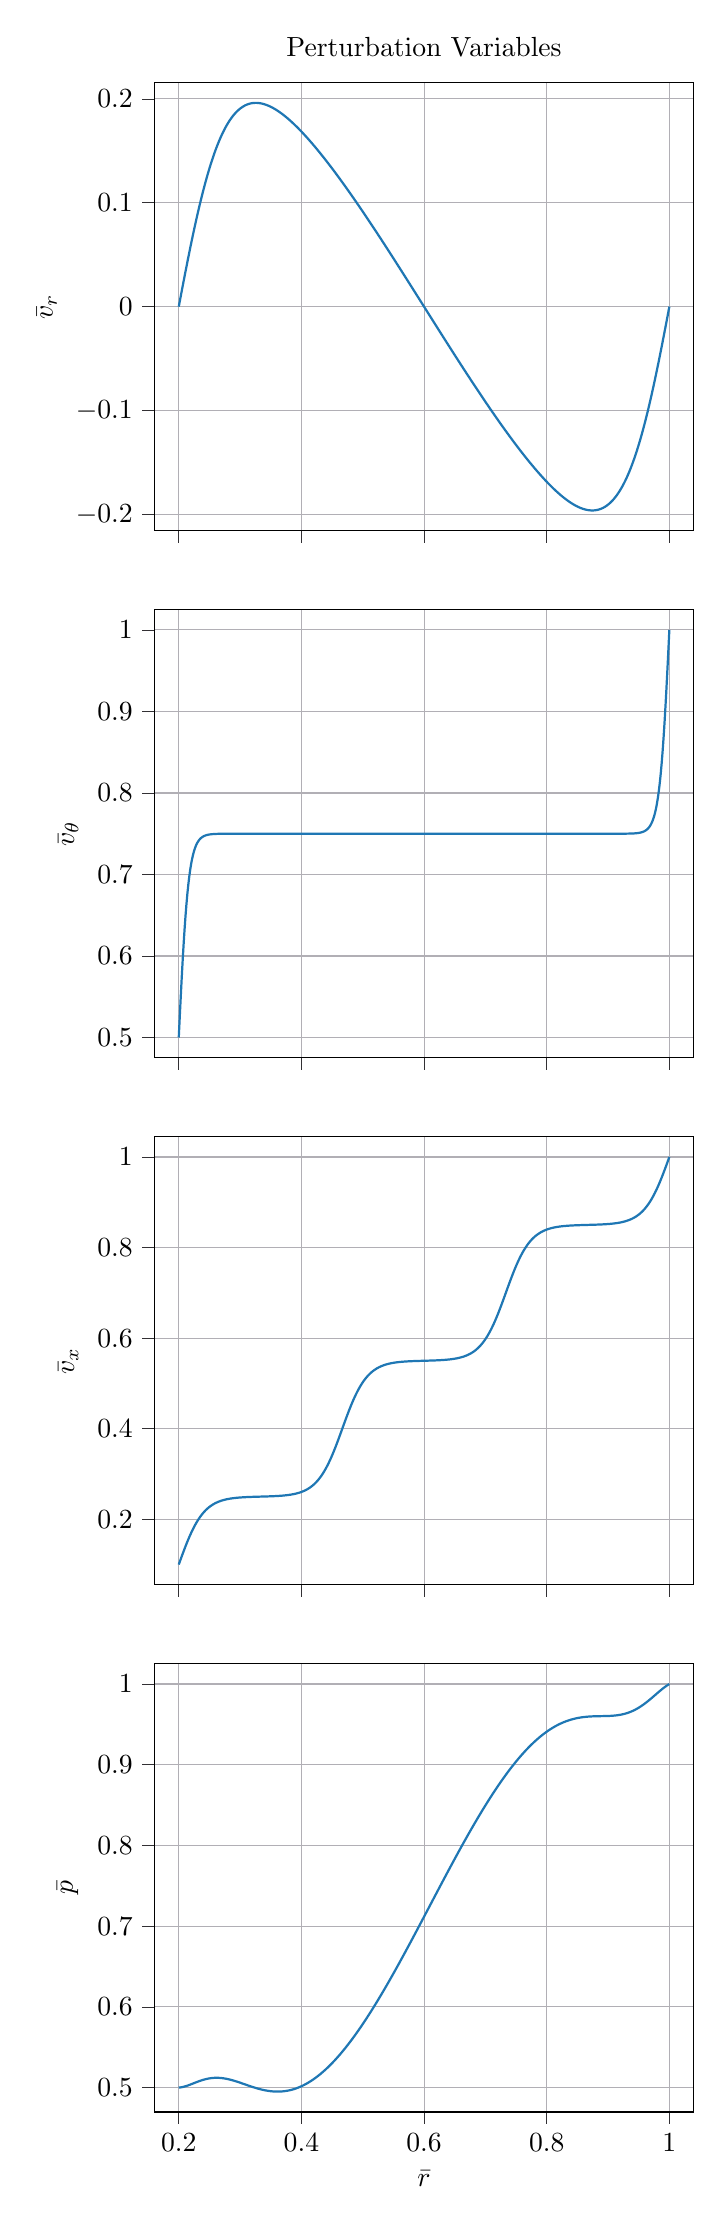
\begin{tikzpicture}

\definecolor{color0}{rgb}{0.196078431372549,0.188235294117647,0.203921568627451}
\definecolor{color1}{rgb}{0.694117647058824,0.686274509803922,0.709803921568627}
\definecolor{color2}{rgb}{0.12156862745098,0.466666666666667,0.705882352941177}

\begin{groupplot}[group style={group size=1 by 4}]
\nextgroupplot[
scaled x ticks=manual:{}{\pgfmathparse{#1}},
tick align=outside,
tick pos=left,
title={Perturbation Variables},
x grid style={color1},
xmajorgrids,
xmin=0.16, xmax=1.04,
xtick style={color=color0},
xticklabels={},
y grid style={color1},
ylabel={\(\displaystyle \bar{v}_r\)},
ymajorgrids,
ymin=-0.215764738330124, ymax=0.215764738330125,
ytick style={color=color0}
]
\addplot [thick, color2]
table {%
0.2 -1.94289029309402e-16
0.2015625 0.00487647715876702
0.203125 0.00973783248093382
0.2046875 0.0145803995642277
0.20625 0.01940053462129
0.2078125 0.0241946276044845
0.209375 0.0289591131137891
0.2109375 0.0336904810192039
0.2125 0.03838528673222
0.2140625 0.0430401610646963
0.215625 0.0476518196179108
0.2171875 0.0522170716495146
0.21875 0.0567328283715534
0.2203125 0.0611961106385339
0.221875 0.0656040559906233
0.2234375 0.0699539250233831
0.225 0.0742431070618588
0.2265625 0.0784691251232999
0.228125 0.0826296401591607
0.2296875 0.0867224545732724
0.23125 0.0907455150190958
0.2328125 0.0946969144846831
0.234375 0.0985748936793645
0.2359375 0.102377841741148
0.2375 0.106104296288355
0.2390625 0.109752942843088
0.240625 0.113322613657662
0.2421875 0.116812285978215
0.24375 0.120221079782228
0.2453125 0.123548255028698
0.246875 0.126793208461235
0.2484375 0.129955470005379
0.25 0.133034698801983
0.2515625 0.13603067891864
0.253125 0.138943314780865
0.2546875 0.141772626364064
0.25625 0.144518744186363
0.2578125 0.147181904141078
0.259375 0.149762442206088
0.2609375 0.152260789065591
0.2625 0.154677464677845
0.2640625 0.157013072820367
0.265625 0.159268295641942
0.2671875 0.161443888248501
0.26875 0.163540673347675
0.2703125 0.165559535974499
0.271875 0.167501418318459
0.2734375 0.169367314669834
0.275 0.171158266501038
0.2765625 0.172875357696604
0.278125 0.174519709943323
0.2796875 0.176092478290177
0.28125 0.177594846885816
0.2828125 0.179028024899616
0.284375 0.180393242630739
0.2859375 0.181691747808131
0.2875 0.182924802083013
0.2890625 0.184093677714198
0.290625 0.185199654445397
0.2921875 0.186244016572712
0.29375 0.187228050199594
0.2953125 0.188153040675747
0.296875 0.189020270215799
0.2984375 0.189831015692955
0.3 0.190586546602362
0.3015625 0.191288123188497
0.303125 0.191936994730582
0.3046875 0.19253439797974
0.30625 0.193081555741456
0.3078125 0.193579675596746
0.309375 0.19402994875539
0.3109375 0.194433549034536
0.3125 0.194791631956037
0.3140625 0.195105333955896
0.315625 0.195375771699333
0.3171875 0.19560404149508
0.31875 0.195791218802663
0.3203125 0.195938357826599
0.321875 0.196046491191628
0.3234375 0.196116629693278
0.325 0.196149762118296
0.3265625 0.196146855129675
0.328125 0.196108853211239
0.3296875 0.196036678666979
0.33125 0.195931231670543
0.3328125 0.195793390360544
0.334375 0.195624010977539
0.3359375 0.195423928038792
0.3375 0.195193954547119
0.3390625 0.19493488223036
0.340625 0.194647481808218
0.3421875 0.194332503283399
0.34375 0.193990676254208
0.3453125 0.193622710245927
0.346875 0.193229295058485
0.3484375 0.192811101128118
0.35 0.192368779900861
0.3515625 0.191902964215906
0.353125 0.19141426869697
0.3546875 0.190903290150006
0.35625 0.190370607965681
0.3578125 0.189816784525223
0.359375 0.189242365608301
0.3609375 0.188647880801778
0.3625 0.188033843908245
0.3640625 0.187400753353344
0.365625 0.186749092591013
0.3671875 0.186079330505846
0.36875 0.185391921811844
0.3703125 0.184687307446936
0.371875 0.183965914962689
0.3734375 0.183228158908707
0.375 0.182474441211286
0.3765625 0.181705151545935
0.378125 0.180920667703438
0.3796875 0.180121355949169
0.38125 0.179307571375433
0.3828125 0.178479658246617
0.384375 0.177637950337022
0.3859375 0.176782771261215
0.3875 0.175914434796846
0.3890625 0.175033245199832
0.390625 0.17413949751189
0.3921875 0.173233477860398
0.39375 0.172315463750589
0.3953125 0.171385724350104
0.396875 0.170444520765946
0.3984375 0.169492106313893
0.4 0.168528726780449
0.4015625 0.1675546206774
0.403125 0.166570019489085
0.4046875 0.165575147912482
0.40625 0.164570224090214
0.4078125 0.163555459836608
0.409375 0.162531060856914
0.4109375 0.161497226959831
0.4125 0.160454152263465
0.4140625 0.159402025394862
0.415625 0.158341029683253
0.4171875 0.157271343347151
0.41875 0.156193139675457
0.4203125 0.155106587202706
0.421875 0.154011849878605
0.4234375 0.152909087232007
0.425 0.151798454529473
0.4265625 0.150680102928555
0.428125 0.149554179625953
0.4296875 0.148420828000687
0.43125 0.147280187752417
0.4328125 0.146132395035064
0.434375 0.144977582585854
0.4359375 0.143815879849936
0.4375 0.142647413100686
0.4390625 0.141472305555852
0.440625 0.140290677489648
0.4421875 0.139102646340932
0.44375 0.137908326817585
0.4453125 0.136707830997222
0.446875 0.135501268424334
0.4484375 0.134288746203998
0.45 0.133070369092245
0.4515625 0.131846239583212
0.453125 0.130616457993171
0.4546875 0.12938112254155
0.45625 0.128140329429035
0.4578125 0.126894172912868
0.459375 0.125642745379409
0.4609375 0.124386137414085
0.4625 0.123124437868794
0.4640625 0.121857733926862
0.465625 0.12058611116563
0.4671875 0.119309653616761
0.46875 0.118028443824344
0.4703125 0.116742562900866
0.471875 0.115452090581134
0.4734375 0.114157105274223
0.475 0.112857684113501
0.4765625 0.111553903004827
0.478125 0.110245836672965
0.4796875 0.108933558706284
0.48125 0.107617141599809
0.4828125 0.106296656796687
0.484375 0.104972174728108
0.4859375 0.103643764851753
0.4875 0.102311495688819
0.4890625 0.100975434859668
0.490625 0.0996356491181564
0.4921875 0.0982922043846861
0.49375 0.0969451657780334
0.4953125 0.0955945976459931
0.496875 0.0942405635948843
0.4984375 0.0928831265179607
0.5 0.0915223486227654
0.5015625 0.0901582914574695
0.503125 0.0887910159362323
0.5046875 0.08742058236362
0.50625 0.086047050458118
0.5078125 0.0846704793747718
0.509375 0.0832909277269866
0.5109375 0.0819084536075219
0.5125 0.080523114608707
0.5140625 0.07913496784191
0.515625 0.0777440699562883
0.5171875 0.0763504771568458
0.51875 0.0749542452218277
0.5203125 0.0735554295194742
0.521875 0.0721540850241596
0.5234375 0.0707502663319415
0.525 0.0693440276755405
0.5265625 0.0679354229387764
0.528125 0.0665245056704775
0.5296875 0.0651113290978875
0.53125 0.0636959461395895
0.5328125 0.0622784094179622
0.534375 0.0608587712711939
0.5359375 0.0594370837648648
0.5375 0.0580133987031207
0.5390625 0.0565877676394513
0.540625 0.0551602418870903
0.5421875 0.0537308725290532
0.54375 0.0522997104278275
0.5453125 0.050866806234729
0.546875 0.0494322103989404
0.5484375 0.0479959731762427
0.55 0.0465581446374553
0.5515625 0.0451187746765963
0.553125 0.0436779130187738
0.5546875 0.0422356092278246
0.55625 0.040791912713705
0.5578125 0.0393468727396515
0.559375 0.0379005384291182
0.5609375 0.0364529587725018
0.5625 0.0350041826336664
0.5640625 0.0335542587562753
0.565625 0.0321032357699408
0.5671875 0.0306511621962022
0.56875 0.0291980864543377
0.5703125 0.0277440568670237
0.571875 0.0262891216658455
0.5734375 0.0248333289966711
0.575 0.0233767269248943
0.5765625 0.0219193634405553
0.578125 0.0204612864633488
0.5796875 0.0190025438475221
0.58125 0.0175431833866773
0.5828125 0.0160832528184791
0.584375 0.0146227998292779
0.5859375 0.0131618720586568
0.5875 0.0117005171039045
0.5890625 0.0102387825244268
0.590625 0.00877671584609932
0.5921875 0.00731436456556861
0.59375 0.00585177615451096
0.5953125 0.00438899806385026
0.596875 0.00292607772794756
0.5984375 0.00146306256876319
0.6 1.94289029309402e-16
0.6015625 -0.00146306256876261
0.603125 -0.00292607772794712
0.6046875 -0.00438899806384979
0.60625 -0.00585177615451038
0.6078125 -0.00731436456556827
0.609375 -0.00877671584609879
0.6109375 -0.0102387825244264
0.6125 -0.0117005171039041
0.6140625 -0.0131618720586562
0.615625 -0.0146227998292776
0.6171875 -0.0160832528184786
0.61875 -0.0175431833866769
0.6203125 -0.0190025438475216
0.621875 -0.0204612864633482
0.6234375 -0.0219193634405551
0.625 -0.0233767269248938
0.6265625 -0.0248333289966707
0.628125 -0.0262891216658451
0.6296875 -0.0277440568670231
0.63125 -0.0291980864543372
0.6328125 -0.0306511621962016
0.634375 -0.0321032357699404
0.6359375 -0.0335542587562749
0.6375 -0.0350041826336658
0.6390625 -0.0364529587725013
0.640625 -0.0379005384291177
0.6421875 -0.039346872739651
0.64375 -0.0407919127137046
0.6453125 -0.042235609227824
0.646875 -0.0436779130187733
0.6484375 -0.0451187746765957
0.65 -0.046558144637455
0.6515625 -0.0479959731762422
0.653125 -0.0494322103989399
0.6546875 -0.0508668062347286
0.65625 -0.0522997104278269
0.6578125 -0.0537308725290527
0.659375 -0.0551602418870898
0.6609375 -0.0565877676394508
0.6625 -0.0580133987031203
0.6640625 -0.0594370837648642
0.665625 -0.0608587712711934
0.6671875 -0.0622784094179618
0.66875 -0.0636959461395888
0.6703125 -0.0651113290978871
0.671875 -0.0665245056704769
0.6734375 -0.0679354229387759
0.675 -0.0693440276755401
0.6765625 -0.0707502663319408
0.678125 -0.0721540850241592
0.6796875 -0.0735554295194736
0.68125 -0.0749542452218271
0.6828125 -0.0763504771568452
0.684375 -0.0777440699562876
0.6859375 -0.0791349678419097
0.6875 -0.0805231146087064
0.6890625 -0.0819084536075214
0.690625 -0.083290927726986
0.6921875 -0.0846704793747712
0.69375 -0.0860470504581175
0.6953125 -0.0874205823636193
0.696875 -0.0887910159362317
0.6984375 -0.090158291457469
0.7 -0.0915223486227648
0.7015625 -0.0928831265179603
0.703125 -0.0942405635948838
0.7046875 -0.0955945976459926
0.70625 -0.096945165778033
0.7078125 -0.0982922043846855
0.709375 -0.0996356491181559
0.7109375 -0.100975434859668
0.7125 -0.102311495688819
0.7140625 -0.103643764851753
0.715625 -0.104972174728108
0.7171875 -0.106296656796687
0.71875 -0.107617141599809
0.7203125 -0.108933558706283
0.721875 -0.110245836672965
0.7234375 -0.111553903004827
0.725 -0.1128576841135
0.7265625 -0.114157105274222
0.728125 -0.115452090581134
0.7296875 -0.116742562900865
0.73125 -0.118028443824343
0.7328125 -0.11930965361676
0.734375 -0.120586111165629
0.7359375 -0.121857733926861
0.7375 -0.123124437868793
0.7390625 -0.124386137414084
0.740625 -0.125642745379408
0.7421875 -0.126894172912867
0.74375 -0.128140329429035
0.7453125 -0.129381122541549
0.746875 -0.130616457993171
0.7484375 -0.131846239583212
0.75 -0.133070369092245
0.7515625 -0.134288746203997
0.753125 -0.135501268424333
0.7546875 -0.136707830997221
0.75625 -0.137908326817585
0.7578125 -0.139102646340932
0.759375 -0.140290677489648
0.7609375 -0.141472305555851
0.7625 -0.142647413100685
0.7640625 -0.143815879849935
0.765625 -0.144977582585854
0.7671875 -0.146132395035063
0.76875 -0.147280187752416
0.7703125 -0.148420828000686
0.771875 -0.149554179625952
0.7734375 -0.150680102928554
0.775 -0.151798454529472
0.7765625 -0.152909087232006
0.778125 -0.154011849878604
0.7796875 -0.155106587202706
0.78125 -0.156193139675456
0.7828125 -0.15727134334715
0.784375 -0.158341029683252
0.7859375 -0.159402025394861
0.7875 -0.160454152263464
0.7890625 -0.16149722695983
0.790625 -0.162531060856913
0.7921875 -0.163555459836608
0.79375 -0.164570224090213
0.7953125 -0.165575147912481
0.796875 -0.166570019489084
0.7984375 -0.167554620677399
0.8 -0.168528726780449
0.8015625 -0.169492106313892
0.803125 -0.170444520765945
0.8046875 -0.171385724350104
0.80625 -0.172315463750589
0.8078125 -0.173233477860397
0.809375 -0.174139497511889
0.8109375 -0.175033245199831
0.8125 -0.175914434796845
0.8140625 -0.176782771261214
0.815625 -0.177637950337021
0.8171875 -0.178479658246616
0.81875 -0.179307571375432
0.8203125 -0.180121355949168
0.821875 -0.180920667703437
0.8234375 -0.181705151545934
0.825 -0.182474441211285
0.8265625 -0.183228158908707
0.828125 -0.183965914962689
0.8296875 -0.184687307446935
0.83125 -0.185391921811843
0.8328125 -0.186079330505845
0.834375 -0.186749092591012
0.8359375 -0.187400753353343
0.8375 -0.188033843908244
0.8390625 -0.188647880801777
0.840625 -0.1892423656083
0.8421875 -0.189816784525222
0.84375 -0.19037060796568
0.8453125 -0.190903290150005
0.846875 -0.191414268696969
0.8484375 -0.191902964215905
0.85 -0.19236877990086
0.8515625 -0.192811101128117
0.853125 -0.193229295058484
0.8546875 -0.193622710245926
0.85625 -0.193990676254207
0.8578125 -0.194332503283398
0.859375 -0.194647481808217
0.8609375 -0.194934882230359
0.8625 -0.195193954547118
0.8640625 -0.195423928038791
0.865625 -0.195624010977538
0.8671875 -0.195793390360543
0.86875 -0.195931231670542
0.8703125 -0.196036678666978
0.871875 -0.196108853211238
0.8734375 -0.196146855129674
0.875 -0.196149762118295
0.8765625 -0.196116629693277
0.878125 -0.196046491191627
0.8796875 -0.195938357826598
0.88125 -0.195791218802662
0.8828125 -0.195604041495079
0.884375 -0.195375771699331
0.8859375 -0.195105333955894
0.8875 -0.194791631956036
0.8890625 -0.194433549034535
0.890625 -0.194029948755388
0.8921875 -0.193579675596745
0.89375 -0.193081555741455
0.8953125 -0.192534397979739
0.896875 -0.191936994730581
0.8984375 -0.191288123188496
0.9 -0.190586546602361
0.9015625 -0.189831015692954
0.903125 -0.189020270215797
0.9046875 -0.188153040675745
0.90625 -0.187228050199592
0.9078125 -0.18624401657271
0.909375 -0.185199654445395
0.9109375 -0.184093677714197
0.9125 -0.182924802083012
0.9140625 -0.181691747808129
0.915625 -0.180393242630738
0.9171875 -0.179028024899615
0.91875 -0.177594846885815
0.9203125 -0.176092478290175
0.921875 -0.174519709943322
0.9234375 -0.172875357696603
0.925 -0.171158266501037
0.9265625 -0.169367314669832
0.928125 -0.167501418318458
0.9296875 -0.165559535974497
0.93125 -0.163540673347674
0.9328125 -0.1614438882485
0.934375 -0.159268295641941
0.9359375 -0.157013072820366
0.9375 -0.154677464677844
0.9390625 -0.152260789065589
0.940625 -0.149762442206086
0.9421875 -0.147181904141077
0.94375 -0.144518744186361
0.9453125 -0.141772626364063
0.946875 -0.138943314780863
0.9484375 -0.136030678918638
0.95 -0.133034698801981
0.9515625 -0.129955470005377
0.953125 -0.126793208461234
0.9546875 -0.123548255028696
0.95625 -0.120221079782227
0.9578125 -0.116812285978213
0.959375 -0.11332261365766
0.9609375 -0.109752942843087
0.9625 -0.106104296288353
0.9640625 -0.102377841741146
0.965625 -0.098574893679363
0.9671875 -0.0946969144846813
0.96875 -0.0907455150190943
0.9703125 -0.0867224545732706
0.971875 -0.082629640159159
0.9734375 -0.0784691251232983
0.975 -0.0742431070618568
0.9765625 -0.0699539250233815
0.978125 -0.0656040559906213
0.9796875 -0.0611961106385321
0.98125 -0.0567328283715516
0.9828125 -0.0522170716495124
0.984375 -0.047651819617909
0.9859375 -0.0430401610646942
0.9875 -0.0383852867322181
0.9890625 -0.0336904810192021
0.990625 -0.0289591131137868
0.9921875 -0.0241946276044828
0.99375 -0.0194005346212877
0.9953125 -0.014580399564226
0.996875 -0.00973783248093213
0.9984375 -0.00487647715876488
1 1.85962356624714e-15
};

\nextgroupplot[
scaled x ticks=manual:{}{\pgfmathparse{#1}},
tick align=outside,
tick pos=left,
x grid style={color1},
xmajorgrids,
xmin=0.16, xmax=1.04,
xtick style={color=color0},
xticklabels={},
y grid style={color1},
ylabel={\(\displaystyle \bar{v}_{\theta}\)},
ymajorgrids,
ymin=0.475, ymax=1.025,
ytick style={color=color0}
]
\addplot [thick, color2]
table {%
0.2 0.5
0.2015625 0.524336747206499
0.203125 0.548216573132313
0.2046875 0.571216238814779
0.20625 0.592974727504097
0.2078125 0.613212804487595
0.209375 0.631741881777146
0.2109375 0.648462685905265
0.2125 0.663355897035337
0.2140625 0.676467739770476
0.215625 0.687893495823973
0.2171875 0.697761338434882
0.21875 0.706218080238471
0.2203125 0.713417639297188
0.221875 0.719512409567518
0.2234375 0.724647317601085
0.225 0.72895613604219
0.2265625 0.73255955653166
0.228125 0.735564546526856
0.2296875 0.738064582523785
0.23125 0.740140435946327
0.2328125 0.741861269543643
0.234375 0.743285872629016
0.2359375 0.744463919908383
0.2375 0.74543718130541
0.2390625 0.746240640969284
0.240625 0.746903504921072
0.2421875 0.747450090848523
0.24375 0.747900602364264
0.2453125 0.748271795165967
0.246875 0.74857754516751
0.2484375 0.748829329674476
0.25 0.749036632668336
0.2515625 0.749207284662089
0.253125 0.749347746676692
0.2546875 0.749463346843545
0.25625 0.749558477076108
0.2578125 0.749636756239342
0.259375 0.749701165314449
0.2609375 0.749754159223854
0.2625 0.749797759251079
0.2640625 0.749833629358296
0.265625 0.749863139163408
0.2671875 0.749887415879072
0.26875 0.749907387128367
0.2703125 0.749923816226163
0.271875 0.749937331242872
0.2734375 0.749948448940146
0.275 0.749957594479138
0.2765625 0.749965117645129
0.278125 0.749971306202393
0.2796875 0.749976396885585
0.28125 0.749980584445066
0.2828125 0.749984029090118
0.284375 0.749986862613428
0.2859375 0.7499891934302
0.2875 0.749991110724068
0.2890625 0.749992687858008
0.290625 0.749993985180458
0.2921875 0.749995052333843
0.29375 0.749995930153688
0.2953125 0.749996652230906
0.296875 0.749997246196988
0.2984375 0.749997734781217
0.3 0.749998136680358
0.3015625 0.749998467274057
0.303125 0.749998739213344
0.3046875 0.749998962904722
0.30625 0.749999146908381
0.3078125 0.749999298265763
0.309375 0.749999422769018
0.3109375 0.749999525182648
0.3125 0.749999609425835
0.3140625 0.74999967872241
0.315625 0.749999735724234
0.3171875 0.749999782612664
0.31875 0.749999821182041
0.3203125 0.74999985290835
0.321875 0.749999879005703
0.3234375 0.749999900472802
0.325 0.749999918131157
0.3265625 0.749999932656525
0.328125 0.749999944604767
0.3296875 0.749999954433123
0.33125 0.749999962517709
0.3328125 0.749999969167908
0.334375 0.749999974638213
0.3359375 0.749999979137962
0.3375 0.749999982839356
0.3390625 0.749999985884039
0.340625 0.749999988388527
0.3421875 0.749999990448663
0.34375 0.749999992143284
0.3453125 0.749999993537242
0.346875 0.74999999468388
0.3484375 0.749999995627079
0.35 0.749999996402933
0.3515625 0.749999997041134
0.353125 0.749999997566103
0.3546875 0.749999997997931
0.35625 0.749999998353143
0.3578125 0.749999998645332
0.359375 0.749999998885681
0.3609375 0.749999999083386
0.3625 0.749999999246014
0.3640625 0.749999999379788
0.365625 0.749999999489827
0.3671875 0.749999999580343
0.36875 0.7499999996548
0.3703125 0.749999999716046
0.371875 0.749999999766426
0.3734375 0.749999999807867
0.375 0.749999999841956
0.3765625 0.749999999869996
0.378125 0.749999999893062
0.3796875 0.749999999912035
0.38125 0.749999999927642
0.3828125 0.74999999994048
0.384375 0.74999999995104
0.3859375 0.749999999959727
0.3875 0.749999999966872
0.3890625 0.74999999997275
0.390625 0.749999999977585
0.3921875 0.749999999981562
0.39375 0.749999999984833
0.3953125 0.749999999987524
0.396875 0.749999999989738
0.3984375 0.749999999991558
0.4 0.749999999993056
0.4015625 0.749999999994288
0.403125 0.749999999995302
0.4046875 0.749999999996135
0.40625 0.749999999996821
0.4078125 0.749999999997385
0.409375 0.749999999997849
0.4109375 0.749999999998231
0.4125 0.749999999998544
0.4140625 0.749999999998803
0.415625 0.749999999999015
0.4171875 0.74999999999919
0.41875 0.749999999999334
0.4203125 0.749999999999452
0.421875 0.749999999999549
0.4234375 0.749999999999629
0.425 0.749999999999695
0.4265625 0.749999999999749
0.428125 0.749999999999793
0.4296875 0.74999999999983
0.43125 0.74999999999986
0.4328125 0.749999999999885
0.434375 0.749999999999906
0.4359375 0.749999999999922
0.4375 0.749999999999936
0.4390625 0.749999999999947
0.440625 0.749999999999957
0.4421875 0.749999999999964
0.44375 0.749999999999971
0.4453125 0.749999999999976
0.446875 0.74999999999998
0.4484375 0.749999999999984
0.45 0.749999999999986
0.4515625 0.749999999999989
0.453125 0.749999999999991
0.4546875 0.749999999999992
0.45625 0.749999999999994
0.4578125 0.749999999999995
0.459375 0.749999999999996
0.4609375 0.749999999999996
0.4625 0.749999999999997
0.4640625 0.749999999999998
0.465625 0.749999999999998
0.4671875 0.749999999999998
0.46875 0.749999999999999
0.4703125 0.749999999999999
0.471875 0.749999999999999
0.4734375 0.749999999999999
0.475 0.749999999999999
0.4765625 0.749999999999999
0.478125 0.749999999999999
0.4796875 0.75
0.48125 0.75
0.4828125 0.75
0.484375 0.75
0.4859375 0.75
0.4875 0.75
0.4890625 0.75
0.490625 0.75
0.4921875 0.75
0.49375 0.75
0.4953125 0.75
0.496875 0.75
0.4984375 0.75
0.5 0.75
0.5015625 0.75
0.503125 0.75
0.5046875 0.75
0.50625 0.75
0.5078125 0.75
0.509375 0.75
0.5109375 0.75
0.5125 0.75
0.5140625 0.75
0.515625 0.75
0.5171875 0.75
0.51875 0.75
0.5203125 0.75
0.521875 0.75
0.5234375 0.75
0.525 0.75
0.5265625 0.75
0.528125 0.75
0.5296875 0.75
0.53125 0.75
0.5328125 0.75
0.534375 0.75
0.5359375 0.75
0.5375 0.75
0.5390625 0.75
0.540625 0.75
0.5421875 0.75
0.54375 0.75
0.5453125 0.75
0.546875 0.75
0.5484375 0.75
0.55 0.75
0.5515625 0.75
0.553125 0.75
0.5546875 0.75
0.55625 0.75
0.5578125 0.75
0.559375 0.75
0.5609375 0.75
0.5625 0.75
0.5640625 0.75
0.565625 0.75
0.5671875 0.75
0.56875 0.75
0.5703125 0.75
0.571875 0.75
0.5734375 0.75
0.575 0.75
0.5765625 0.75
0.578125 0.75
0.5796875 0.75
0.58125 0.75
0.5828125 0.75
0.584375 0.75
0.5859375 0.75
0.5875 0.75
0.5890625 0.75
0.590625 0.75
0.5921875 0.75
0.59375 0.75
0.5953125 0.75
0.596875 0.75
0.5984375 0.75
0.6 0.75
0.6015625 0.75
0.603125 0.75
0.6046875 0.75
0.60625 0.75
0.6078125 0.75
0.609375 0.75
0.6109375 0.75
0.6125 0.75
0.6140625 0.75
0.615625 0.75
0.6171875 0.75
0.61875 0.75
0.6203125 0.75
0.621875 0.75
0.6234375 0.75
0.625 0.75
0.6265625 0.75
0.628125 0.75
0.6296875 0.75
0.63125 0.75
0.6328125 0.75
0.634375 0.75
0.6359375 0.75
0.6375 0.75
0.6390625 0.75
0.640625 0.75
0.6421875 0.75
0.64375 0.75
0.6453125 0.75
0.646875 0.75
0.6484375 0.75
0.65 0.75
0.6515625 0.75
0.653125 0.75
0.6546875 0.75
0.65625 0.75
0.6578125 0.75
0.659375 0.75
0.6609375 0.75
0.6625 0.75
0.6640625 0.75
0.665625 0.75
0.6671875 0.75
0.66875 0.75
0.6703125 0.75
0.671875 0.75
0.6734375 0.75
0.675 0.75
0.6765625 0.75
0.678125 0.75
0.6796875 0.75
0.68125 0.75
0.6828125 0.75
0.684375 0.75
0.6859375 0.75
0.6875 0.75
0.6890625 0.75
0.690625 0.75
0.6921875 0.75
0.69375 0.75
0.6953125 0.75
0.696875 0.75
0.6984375 0.75
0.7 0.75
0.7015625 0.75
0.703125 0.75
0.7046875 0.75
0.70625 0.75
0.7078125 0.75
0.709375 0.75
0.7109375 0.75
0.7125 0.75
0.7140625 0.75
0.715625 0.75
0.7171875 0.75
0.71875 0.75
0.7203125 0.75
0.721875 0.75
0.7234375 0.75
0.725 0.750000000000001
0.7265625 0.750000000000001
0.728125 0.750000000000001
0.7296875 0.750000000000001
0.73125 0.750000000000001
0.7328125 0.750000000000002
0.734375 0.750000000000002
0.7359375 0.750000000000002
0.7375 0.750000000000003
0.7390625 0.750000000000003
0.740625 0.750000000000004
0.7421875 0.750000000000005
0.74375 0.750000000000006
0.7453125 0.750000000000007
0.746875 0.750000000000009
0.7484375 0.750000000000011
0.75 0.750000000000013
0.7515625 0.750000000000016
0.753125 0.75000000000002
0.7546875 0.750000000000024
0.75625 0.750000000000029
0.7578125 0.750000000000036
0.759375 0.750000000000043
0.7609375 0.750000000000053
0.7625 0.750000000000064
0.7640625 0.750000000000078
0.765625 0.750000000000094
0.7671875 0.750000000000115
0.76875 0.75000000000014
0.7703125 0.75000000000017
0.771875 0.750000000000207
0.7734375 0.750000000000251
0.775 0.750000000000305
0.7765625 0.750000000000371
0.778125 0.750000000000451
0.7796875 0.750000000000548
0.78125 0.750000000000666
0.7828125 0.75000000000081
0.784375 0.750000000000985
0.7859375 0.750000000001197
0.7875 0.750000000001456
0.7890625 0.750000000001769
0.790625 0.750000000002151
0.7921875 0.750000000002615
0.79375 0.750000000003179
0.7953125 0.750000000003865
0.796875 0.750000000004698
0.7984375 0.750000000005712
0.8 0.750000000006944
0.8015625 0.750000000008442
0.803125 0.750000000010262
0.8046875 0.750000000012476
0.80625 0.750000000015167
0.8078125 0.750000000018438
0.809375 0.750000000022415
0.8109375 0.75000000002725
0.8125 0.750000000033128
0.8140625 0.750000000040273
0.815625 0.75000000004896
0.8171875 0.75000000005952
0.81875 0.750000000072358
0.8203125 0.750000000087965
0.821875 0.750000000106938
0.8234375 0.750000000130003
0.825 0.750000000158044
0.8265625 0.750000000192133
0.828125 0.750000000233574
0.8296875 0.750000000283954
0.83125 0.7500000003452
0.8328125 0.750000000419657
0.834375 0.750000000510172
0.8359375 0.750000000620212
0.8375 0.750000000753986
0.8390625 0.750000000916614
0.840625 0.750000001114319
0.8421875 0.750000001354668
0.84375 0.750000001646857
0.8453125 0.750000002002069
0.846875 0.750000002433897
0.8484375 0.750000002958866
0.85 0.750000003597066
0.8515625 0.750000004372921
0.853125 0.75000000531612
0.8546875 0.750000006462758
0.85625 0.750000007856716
0.8578125 0.750000009551337
0.859375 0.750000011611473
0.8609375 0.750000014115961
0.8625 0.750000017160644
0.8640625 0.750000020862037
0.865625 0.750000025361787
0.8671875 0.750000030832092
0.86875 0.750000037482291
0.8703125 0.750000045566877
0.871875 0.750000055395233
0.8734375 0.750000067343475
0.875 0.750000081868843
0.8765625 0.750000099527198
0.878125 0.750000120994297
0.8796875 0.75000014709165
0.88125 0.750000178817959
0.8828125 0.750000217387336
0.884375 0.750000264275766
0.8859375 0.750000321277589
0.8875 0.750000390574165
0.8890625 0.750000474817351
0.890625 0.750000577230982
0.8921875 0.750000701734237
0.89375 0.750000853091619
0.8953125 0.750001037095278
0.896875 0.750001260786655
0.8984375 0.750001532725943
0.9 0.750001863319642
0.9015625 0.750002265218782
0.903125 0.750002753803012
0.9046875 0.750003347769094
0.90625 0.750004069846312
0.9078125 0.750004947666157
0.909375 0.750006014819542
0.9109375 0.750007312141992
0.9125 0.750008889275931
0.9140625 0.7500108065698
0.915625 0.750013137386572
0.9171875 0.750015970909882
0.91875 0.750019415554934
0.9203125 0.750023603114415
0.921875 0.750028693797607
0.9234375 0.750034882354871
0.925 0.750042405520862
0.9265625 0.750051551059853
0.928125 0.750062668757128
0.9296875 0.750076183773837
0.93125 0.750092612871633
0.9328125 0.750112584120928
0.934375 0.750136860836592
0.9359375 0.750166370641703
0.9375 0.750202240748921
0.9390625 0.750245840776146
0.940625 0.750298834685551
0.9421875 0.750363243760658
0.94375 0.750441522923892
0.9453125 0.750536653156455
0.946875 0.750652253323308
0.9484375 0.75079271533791
0.95 0.750963367331664
0.9515625 0.751170670325524
0.953125 0.75142245483249
0.9546875 0.751728204834033
0.95625 0.752099397635736
0.9578125 0.752549909151477
0.959375 0.753096495078928
0.9609375 0.753759359030716
0.9625 0.75456281869459
0.9640625 0.755536080091617
0.965625 0.756714127370984
0.9671875 0.758138730456357
0.96875 0.759859564053673
0.9703125 0.761935417476216
0.971875 0.764435453473144
0.9734375 0.76744044346834
0.975 0.77104386395781
0.9765625 0.775352682398915
0.978125 0.780487590432483
0.9796875 0.786582360702812
0.98125 0.793781919761529
0.9828125 0.802238661565119
0.984375 0.812106504176027
0.9859375 0.823532260229525
0.9875 0.836644102964663
0.9890625 0.851537314094735
0.990625 0.868258118222855
0.9921875 0.886787195512405
0.99375 0.907025272495905
0.9953125 0.928783761185221
0.996875 0.951783426867687
0.9984375 0.975663252793502
1 1
};

\nextgroupplot[
scaled x ticks=manual:{}{\pgfmathparse{#1}},
tick align=outside,
tick pos=left,
x grid style={color1},
xmajorgrids,
xmin=0.16, xmax=1.04,
xtick style={color=color0},
xticklabels={},
y grid style={color1},
ylabel={\(\displaystyle \bar{v}_x\)},
ymajorgrids,
ymin=0.0550010203459795, ymax=1.0449999514121,
ytick style={color=color0}
]
\addplot [thick, color2]
table {%
0.2 0.100000971758076
0.2015625 0.1058574078251
0.203125 0.111696020135333
0.2046875 0.117499198388043
0.20625 0.123249759552291
0.2078125 0.128931147840538
0.209375 0.134527618965598
0.2109375 0.140024404505094
0.2125 0.145407853019126
0.2140625 0.150665545491355
0.215625 0.155786383636848
0.2171875 0.160760650587906
0.21875 0.165580044382761
0.2203125 0.170237685500309
0.221875 0.174728100375655
0.2234375 0.179047183376412
0.225 0.183192140109083
0.2265625 0.187161415160034
0.228125 0.190954607466041
0.2296875 0.194572376471644
0.23125 0.198016342085332
0.2328125 0.201288981216929
0.234375 0.204393523387973
0.2359375 0.207333847577805
0.2375 0.210114382120679
0.2390625 0.212740009120664
0.240625 0.215215974515363
0.2421875 0.217547804606975
0.24375 0.219741229597246
0.2453125 0.221802114415759
0.246875 0.223736396920712
0.2484375 0.225550033377746
0.25 0.227248950983906
0.2515625 0.228839007097832
0.253125 0.230325954760363
0.2546875 0.231715414038271
0.25625 0.233012848693911
0.2578125 0.234223547671575
0.259375 0.235352610893618
0.2609375 0.236404938872975
0.2625 0.237385225670565
0.2640625 0.238297954753911
0.265625 0.239147397345054
0.2671875 0.239937612879825
0.26875 0.240672451235368
0.2703125 0.241355556417503
0.271875 0.241990371433198
0.2734375 0.242580144105591
0.275 0.243127933619194
0.2765625 0.243636617610912
0.278125 0.244108899648194
0.2796875 0.244547316958932
0.28125 0.244954248298701
0.2828125 0.245331921859647
0.284375 0.245682423141885
0.2859375 0.24600770272288
0.2875 0.246309583872973
0.2890625 0.246589769976302
0.290625 0.246849851725852
0.2921875 0.247091314069552
0.29375 0.247315542891244
0.2953125 0.247523831416236
0.296875 0.247717386336026
0.2984375 0.247897333650893
0.3 0.248064724232389
0.3015625 0.248220539110526
0.303125 0.248365694492634
0.3046875 0.248501046522647
0.30625 0.248627395790906
0.3078125 0.248745491605655
0.309375 0.248856036038117
0.3109375 0.248959687753646
0.3125 0.249057065641773
0.3140625 0.249148752258189
0.315625 0.249235297091807
0.3171875 0.249317219670061
0.31875 0.24939501251549
0.3203125 0.249469143966603
0.321875 0.249540060875793
0.3234375 0.249608191196965
0.325 0.249673946475294
0.3265625 0.249737724251382
0.328125 0.249799910391895
0.3296875 0.249860881358571
0.33125 0.249921006427379
0.3328125 0.24998064986945
0.334375 0.250040173105324
0.3359375 0.250099936843964
0.3375 0.250160303217975
0.3390625 0.250221637926427
0.340625 0.250284312396717
0.3421875 0.25034870597696
0.34375 0.250415208170465
0.3453125 0.25048422092398
0.346875 0.250556160981497
0.3484375 0.2506314623156
0.35 0.25071057864848
0.3515625 0.250793986074929
0.353125 0.250882185799835
0.3546875 0.250975707002854
0.35625 0.251075109843129
0.3578125 0.25118098861705
0.359375 0.251293975082171
0.3609375 0.251414741960426
0.3625 0.251544006633778
0.3640625 0.251682535045267
0.365625 0.251831145818213
0.3671875 0.251990714605859
0.36875 0.252162178683149
0.3703125 0.252346541791486
0.371875 0.25254487924615
0.3734375 0.252758343314587
0.375 0.252988168871866
0.3765625 0.253235679337259
0.378125 0.253502292892916
0.3796875 0.253789528982063
0.38125 0.254099015079777
0.3828125 0.254432493724197
0.384375 0.254791829789832
0.3859375 0.255179017977273
0.3875 0.255596190485079
0.3890625 0.256045624819533
0.390625 0.256529751686413
0.3921875 0.257051162895595
0.39375 0.257612619194055
0.3953125 0.258217057925584
0.396875 0.258867600396076
0.3984375 0.259567558801499
0.4 0.260320442551563
0.4015625 0.261129963795653
0.403125 0.262000041928813
0.4046875 0.26293480682471
0.40625 0.263938600509765
0.4078125 0.265015976958547
0.409375 0.266171699655693
0.4109375 0.267410736534924
0.4125 0.268738251872331
0.4140625 0.270159594680462
0.415625 0.271680283123636
0.4171875 0.273305984455522
0.41875 0.275042489969903
0.4203125 0.27689568445766
0.421875 0.278871509680546
0.4234375 0.280975921409066
0.425 0.283214839631266
0.4265625 0.285594091625433
0.428125 0.288119347706216
0.4296875 0.290796049603564
0.43125 0.29362933161964
0.4328125 0.296623934931451
0.434375 0.29978411566606
0.4359375 0.303113547667948
0.4375 0.306615221199344
0.4390625 0.310291339155675
0.440625 0.314143212728151
0.4421875 0.318171158788875
0.44375 0.322374401592489
0.4453125 0.326750981661187
0.446875 0.331297674924075
0.4484375 0.336009925293734
0.45 0.340881793859983
0.4515625 0.345905927743656
0.453125 0.351073551367352
0.4546875 0.356374482458426
0.45625 0.361797174504026
0.4578125 0.367328786641304
0.459375 0.372955281111918
0.4609375 0.378661547473153
0.4625 0.384431551782623
0.4640625 0.390248508010488
0.465625 0.396095068036966
0.4671875 0.401953525817337
0.46875 0.407806030690143
0.4703125 0.413634804406248
0.471875 0.419422356292882
0.4734375 0.425151691048889
0.475 0.430806503989463
0.4765625 0.436371359099426
0.478125 0.441831845978384
0.4796875 0.447174712622813
0.48125 0.452387971937016
0.4828125 0.457460980842033
0.484375 0.462384491806544
0.4859375 0.46715067750977
0.4875 0.471753130125375
0.4890625 0.476186837359812
0.490625 0.480448137872296
0.4921875 0.484534659040937
0.49375 0.4884452402251
0.4953125 0.492179844719664
0.496875 0.495739463520866
0.4984375 0.499126013847402
0.5 0.502342235107934
0.5015625 0.505391584700328
0.503125 0.508278135690666
0.5046875 0.511006478070522
0.50625 0.513581624945372
0.5078125 0.516008924677969
0.509375 0.518293979707569
0.5109375 0.520442572495173
0.5125 0.522460598810009
0.5140625 0.524354008374522
0.515625 0.526128752723478
0.5171875 0.527790740005493
0.51875 0.529345796359384
0.5203125 0.53079963342974
0.521875 0.532157821542242
0.5234375 0.533425768035714
0.525 0.534608700241011
0.5265625 0.53571165260326
0.528125 0.536739457460527
0.5296875 0.537696739016162
0.53125 0.538587910071371
0.5328125 0.539417171117261
0.534375 0.540188511419986
0.5359375 0.540905711767512
0.5375 0.541572348580968
0.5390625 0.542191799126767
0.540625 0.542767247597227
0.5421875 0.543301691856927
0.54375 0.543797950679229
0.5453125 0.544258671322349
0.546875 0.544686337316801
0.5484375 0.545083276356329
0.55 0.54545166820235
0.5515625 0.545793552527879
0.553125 0.546110836640829
0.5546875 0.54640530303872
0.55625 0.54667861675737
0.5578125 0.546932332485177
0.559375 0.547167901422349
0.5609375 0.547386677870958
0.5625 0.547589925547289
0.5640625 0.547778823612494
0.565625 0.547954472421456
0.5671875 0.548117898992873
0.56875 0.54827006220614
0.5703125 0.54841185773265
0.571875 0.548544122710742
0.5734375 0.548667640174801
0.575 0.548783143249924
0.5765625 0.548891319124299
0.578125 0.54899281281188
0.5796875 0.5490882307183
0.58125 0.54917814402309
0.5828125 0.549263091891365
0.584375 0.549343584528111
0.5859375 0.549420106088098
0.5875 0.54949311745435
0.5890625 0.549563058897913
0.590625 0.549630352631483
0.5921875 0.549695405269282
0.59375 0.549758610205382
0.5953125 0.549820349922481
0.596875 0.549880998243003
0.5984375 0.549940922534224
0.6 0.550000485879038
0.6015625 0.550060049223852
0.603125 0.550119973515073
0.6046875 0.550180621835595
0.60625 0.550242361552694
0.6078125 0.550305566488794
0.609375 0.550370619126593
0.6109375 0.550437912860163
0.6125 0.550507854303726
0.6140625 0.550580865669979
0.615625 0.550657387229965
0.6171875 0.550737879866711
0.61875 0.550822827734986
0.6203125 0.550912741039776
0.621875 0.551008158946196
0.6234375 0.551109652633777
0.625 0.551217828508152
0.6265625 0.551333331583275
0.628125 0.551456849047334
0.6296875 0.551589114025426
0.63125 0.551730909551936
0.6328125 0.551883072765203
0.634375 0.55204649933662
0.6359375 0.552222148145582
0.6375 0.552411046210787
0.6390625 0.552614293887118
0.640625 0.552833070335727
0.6421875 0.553068639272899
0.64375 0.553322355000706
0.6453125 0.553595668719356
0.646875 0.553890135117247
0.6484375 0.554207419230197
0.65 0.554549303555726
0.6515625 0.554917695401747
0.653125 0.555314634441275
0.6546875 0.555742300435728
0.65625 0.556203021078847
0.6578125 0.556699279901149
0.659375 0.557233724160849
0.6609375 0.557809172631309
0.6625 0.558428623177108
0.6640625 0.559095259990564
0.665625 0.55981246033809
0.6671875 0.560583800640815
0.66875 0.561413061686705
0.6703125 0.562304232741914
0.671875 0.563261514297548
0.6734375 0.564289319154816
0.675 0.565392271517065
0.6765625 0.566575203722362
0.678125 0.567843150215834
0.6796875 0.569201338328336
0.68125 0.570655175398692
0.6828125 0.572210231752583
0.684375 0.573872219034598
0.6859375 0.575646963383554
0.6875 0.577540372948067
0.6890625 0.579558399262903
0.690625 0.581706992050507
0.6921875 0.583992047080107
0.69375 0.586419346812704
0.6953125 0.588994493687554
0.696875 0.59172283606741
0.6984375 0.594609387057748
0.7 0.597658736650142
0.7015625 0.600874957910674
0.703125 0.60426150823721
0.7046875 0.607821127038412
0.70625 0.611555731532976
0.7078125 0.615466312717139
0.709375 0.61955283388578
0.7109375 0.623814134398263
0.7125 0.628247841632702
0.7140625 0.632850294248305
0.715625 0.637616479951532
0.7171875 0.642539990916043
0.71875 0.647612999821059
0.7203125 0.652826259135263
0.721875 0.658169125779691
0.7234375 0.663629612658649
0.725 0.669194467768613
0.7265625 0.674849280709186
0.728125 0.680578615465195
0.7296875 0.686366167351828
0.73125 0.692194941067932
0.7328125 0.698047445940739
0.734375 0.703905903721109
0.7359375 0.709752463747589
0.7375 0.715569419975453
0.7390625 0.721339424284923
0.740625 0.727045690646158
0.7421875 0.732672185116771
0.74375 0.73820379725405
0.7453125 0.743626489299649
0.746875 0.748927420390724
0.7484375 0.75409504401442
0.75 0.759119177898092
0.7515625 0.763991046464342
0.753125 0.768703296834001
0.7546875 0.773249990096889
0.75625 0.777626570165587
0.7578125 0.781829812969201
0.759375 0.785857759029926
0.7609375 0.789709632602401
0.7625 0.793385750558732
0.7640625 0.796887424090128
0.765625 0.800216856092015
0.7671875 0.803377036826625
0.76875 0.806371640138436
0.7703125 0.809204922154511
0.771875 0.811881624051861
0.7734375 0.814406880132643
0.775 0.81678613212681
0.7765625 0.81902505034901
0.778125 0.82112946207753
0.7796875 0.823105287300416
0.78125 0.824958481788172
0.7828125 0.826694987302555
0.784375 0.82832068863444
0.7859375 0.829841377077614
0.7875 0.831262719885745
0.7890625 0.832590235223152
0.790625 0.833829272102383
0.7921875 0.834984994799529
0.79375 0.836062371248311
0.7953125 0.837066164933366
0.796875 0.838000929829263
0.7984375 0.838871007962423
0.8 0.839680529206513
0.8015625 0.840433412956577
0.803125 0.841133371362
0.8046875 0.841783913832492
0.80625 0.842388352564021
0.8078125 0.842949808862481
0.809375 0.843471220071663
0.8109375 0.843955346938543
0.8125 0.844404781272996
0.8140625 0.844821953780803
0.815625 0.845209141968244
0.8171875 0.845568478033879
0.81875 0.845901956678299
0.8203125 0.846211442776013
0.821875 0.84649867886516
0.8234375 0.846765292420817
0.825 0.84701280288621
0.8265625 0.84724262844349
0.828125 0.847456092511926
0.8296875 0.84765442996659
0.83125 0.847838793074927
0.8328125 0.848010257152217
0.834375 0.848169825939863
0.8359375 0.848318436712809
0.8375 0.848456965124298
0.8390625 0.84858622979765
0.840625 0.848706996675905
0.8421875 0.848819983141026
0.84375 0.848925861914947
0.8453125 0.849025264755222
0.846875 0.849118785958241
0.8484375 0.849206985683146
0.85 0.849290393109596
0.8515625 0.849369509442476
0.853125 0.849444810776579
0.8546875 0.849516750834096
0.85625 0.849585763587611
0.8578125 0.849652265781116
0.859375 0.849716659361359
0.8609375 0.849779333831649
0.8625 0.849840668540101
0.8640625 0.849901034914112
0.865625 0.849960798652752
0.8671875 0.850020321888626
0.86875 0.850079965330697
0.8703125 0.850140090399505
0.871875 0.850201061366181
0.8734375 0.850263247506694
0.875 0.850327025282782
0.8765625 0.850392780561111
0.878125 0.850460910882283
0.8796875 0.850531827791473
0.88125 0.850605959242586
0.8828125 0.850683752088015
0.884375 0.850765674666269
0.8859375 0.850852219499887
0.8875 0.850943906116303
0.8890625 0.85104128400443
0.890625 0.851144935719959
0.8921875 0.851255480152421
0.89375 0.85137357596717
0.8953125 0.85149992523543
0.896875 0.851635277265442
0.8984375 0.85178043264755
0.9 0.851936247525687
0.9015625 0.852103638107183
0.903125 0.85228358542205
0.9046875 0.85247714034184
0.90625 0.852685428866832
0.9078125 0.852909657688524
0.909375 0.853151120032224
0.9109375 0.853411201781774
0.9125 0.853691387885103
0.9140625 0.853993269035196
0.915625 0.854318548616191
0.9171875 0.854669049898429
0.91875 0.855046723459375
0.9203125 0.855453654799144
0.921875 0.855892072109882
0.9234375 0.856364354147164
0.925 0.856873038138882
0.9265625 0.857420827652486
0.928125 0.858010600324878
0.9296875 0.858645415340573
0.93125 0.859328520522708
0.9328125 0.860063358878251
0.934375 0.860853574413022
0.9359375 0.861703017004165
0.9375 0.862615746087511
0.9390625 0.863596032885101
0.940625 0.864648360864458
0.9421875 0.865777424086501
0.94375 0.866988123064165
0.9453125 0.868285557719805
0.946875 0.869675016997713
0.9484375 0.871161964660244
0.95 0.87275202077417
0.9515625 0.87445093838033
0.953125 0.876264574837364
0.9546875 0.878198857342317
0.95625 0.88025974216083
0.9578125 0.882453167151101
0.959375 0.884784997242714
0.9609375 0.887260962637412
0.9625 0.889886589637397
0.9640625 0.892667124180271
0.965625 0.895607448370103
0.9671875 0.898711990541147
0.96875 0.901984629672744
0.9703125 0.905428595286433
0.971875 0.909046364292035
0.9734375 0.912839556598042
0.975 0.916808831648994
0.9765625 0.920953788381664
0.978125 0.925272871382421
0.9796875 0.929763286257767
0.98125 0.934420927375314
0.9828125 0.939240321170171
0.984375 0.944214588121228
0.9859375 0.949335426266722
0.9875 0.95459311873895
0.9890625 0.959976567252982
0.990625 0.965473352792479
0.9921875 0.971069823917538
0.99375 0.976751212205786
0.9953125 0.982501773370034
0.996875 0.988304951622743
0.9984375 0.994143563932977
1 1
};

\nextgroupplot[
tick align=outside,
tick pos=left,
x grid style={color1},
xlabel={\(\displaystyle \bar{r}\)},
xmajorgrids,
xmin=0.16, xmax=1.04,
xtick style={color=color0},
y grid style={color1},
ylabel={\(\displaystyle \bar{p}\)},
ymajorgrids,
ymin=0.469783543166816, ymax=1.02524840270631,
ytick style={color=color0}
]
\addplot [thick, color2]
table {%
0.2 0.500000002061149
0.2015625 0.500104235222132
0.203125 0.500258510981381
0.2046875 0.500458911970661
0.20625 0.500701543436648
0.2078125 0.500982544365744
0.209375 0.501298098391962
0.2109375 0.501644444419342
0.2125 0.502017886893408
0.2140625 0.502414805660058
0.215625 0.502831665354607
0.2171875 0.503265024268741
0.21875 0.503711542648544
0.2203125 0.504167990382559
0.221875 0.50463125404499
0.2234375 0.505098343265434
0.225 0.505566396402975
0.2265625 0.506032685508899
0.228125 0.506494620568696
0.2296875 0.506949753020234
0.23125 0.507395778551012
0.2328125 0.507830539183118
0.234375 0.508252024659918
0.2359375 0.508658373153458
0.2375 0.509047871316096
0.2390625 0.509418953703971
0.240625 0.509770201603434
0.2421875 0.510100341294661
0.24375 0.510408241789169
0.2453125 0.510692912079992
0.246875 0.510953497944777
0.2484375 0.5111892783431
0.25 0.51139966144985
0.2515625 0.51158418036666
0.253125 0.511742488553078
0.2546875 0.511874355018549
0.25625 0.511979659315235
0.2578125 0.512058386370489
0.259375 0.512110621196225
0.2609375 0.512136543510681
0.2625 0.512136422306149
0.2640625 0.512110610394185
0.265625 0.512059538957608
0.2671875 0.511983712136387
0.26875 0.511883701672191
0.2703125 0.51176014163409
0.271875 0.511613723245608
0.2734375 0.511445189831058
0.275 0.511255331896896
0.2765625 0.511044982361686
0.278125 0.510815011946259
0.2796875 0.510566324733633
0.28125 0.510299853906495
0.2828125 0.510016557668258
0.284375 0.50971741535212
0.2859375 0.509403423721063
0.2875 0.509075593460347
0.2890625 0.508734945862819
0.290625 0.508382509706228
0.2921875 0.508019318320714
0.29375 0.507646406843763
0.2953125 0.507264809659117
0.296875 0.50687555801544
0.2984375 0.506479677819974
0.3 0.506078187601902
0.3015625 0.505672096639738
0.303125 0.505262403246741
0.3046875 0.504850093208072
0.30625 0.504436138363249
0.3078125 0.504021495327329
0.309375 0.503607104344126
0.3109375 0.503193888264827
0.3125 0.50278275164532
0.3140625 0.502374579955644
0.315625 0.501970238895058
0.3171875 0.501570573806329
0.31875 0.501176409183021
0.3203125 0.500788548263687
0.321875 0.500407772707103
0.3234375 0.500034842342834
0.325 0.499670494991665
0.3265625 0.499315446350625
0.328125 0.498970389937576
0.3296875 0.498635997090543
0.33125 0.498312917017212
0.3328125 0.498001776890233
0.334375 0.4977031819842
0.3359375 0.497417715850414
0.3375 0.497145940525726
0.3390625 0.496888396772015
0.340625 0.496645604343019
0.3421875 0.49641806227548
0.34375 0.496206249201742
0.3453125 0.496010623681123
0.346875 0.495831624547589
0.3484375 0.495669671271411
0.35 0.495525164332663
0.3515625 0.495398485604572
0.353125 0.495289998744893
0.3546875 0.495200049593614
0.35625 0.495128966575442
0.3578125 0.495077061105638
0.359375 0.495044627997909
0.3609375 0.495031945873157
0.3625 0.495039277568006
0.3640625 0.495066870542137
0.365625 0.495114957283525
0.3671875 0.495183755710799
0.36875 0.495273469571998
0.3703125 0.495384288839088
0.371875 0.495516390097672
0.3734375 0.495669936931391
0.375 0.495845080300577
0.3765625 0.496041958914777
0.378125 0.496260699598811
0.3796875 0.496501417652091
0.38125 0.496764217200955
0.3828125 0.497049191543832
0.384375 0.497356423489055
0.3859375 0.497685985685231
0.3875 0.498037940944045
0.3890625 0.498412342555452
0.390625 0.498809234595204
0.3921875 0.499228652224717
0.39375 0.499670621983262
0.3953125 0.500135162072514
0.396875 0.500622282633513
0.3984375 0.501131986016076
0.4 0.501664267040742
0.4015625 0.502219113253333
0.403125 0.502796505172227
0.4046875 0.503396416528437
0.40625 0.504018814498624
0.4078125 0.504663659931151
0.409375 0.505330907565305
0.4109375 0.50602050624382
0.4125 0.506732399118842
0.4140625 0.507466523851451
0.415625 0.508222812804916
0.4171875 0.509001193231786
0.41875 0.509801587455
0.4203125 0.510623913043129
0.421875 0.511468082979916
0.4234375 0.512334005828251
0.425 0.513221585888732
0.4265625 0.514130723352949
0.428125 0.515061314451637
0.4296875 0.516013251597853
0.43125 0.516986423525294
0.4328125 0.517980715421918
0.434375 0.518996009058989
0.4359375 0.520032182915689
0.4375 0.521089112299433
0.4390625 0.522166669462007
0.440625 0.523264723711661
0.4421875 0.524383141521288
0.44375 0.525521786632806
0.4453125 0.526680520157868
0.446875 0.527859200675002
0.4484375 0.529057684323321
0.45 0.530275824892893
0.4515625 0.531513473911891
0.453125 0.532770480730625
0.4546875 0.534046692602558
0.45625 0.535341954762415
0.4578125 0.536656110501472
0.459375 0.537989001240128
0.4609375 0.539340466597846
0.4625 0.540710344460561
0.4640625 0.542098471045635
0.465625 0.543504680964446
0.4671875 0.544928807282694
0.46875 0.546370681578505
0.4703125 0.547830133998401
0.471875 0.549306993311229
0.4734375 0.550801086960097
0.475 0.552312241112413
0.4765625 0.553840280708071
0.478125 0.555385029505871
0.4796875 0.55694631012822
0.48125 0.55852394410418
0.4828125 0.560117751910935
0.484375 0.561727553013709
0.4859375 0.563353165904222
0.4875 0.564994408137709
0.4890625 0.566651096368566
0.490625 0.568323046384686
0.4921875 0.570010073140511
0.49375 0.571711990788851
0.4953125 0.573428612711538
0.496875 0.575159751548929
0.4984375 0.576905219228314
0.5 0.578664826991272
0.5015625 0.580438385420011
0.503125 0.582225704462728
0.5046875 0.584026593458025
0.50625 0.585840861158425
0.5078125 0.587668315753009
0.509375 0.58950876488922
0.5109375 0.591362015693854
0.5125 0.593227874793276
0.5140625 0.595106148332893
0.515625 0.596996641995897
0.5171875 0.59889916102133
0.51875 0.600813510221473
0.5203125 0.602739493998603
0.521875 0.604676916361133
0.5234375 0.606625580939154
0.525 0.608585290999426
0.5265625 0.610555849459804
0.528125 0.612537058903154
0.5296875 0.614528721590756
0.53125 0.61653063947523
0.5328125 0.618542614212992
0.534375 0.620564447176265
0.5359375 0.622595939464667
0.5375 0.624636891916383
0.5390625 0.626687105118935
0.540625 0.628746379419597
0.5421875 0.630814514935419
0.54375 0.632891311562926
0.5453125 0.634976568987472
0.546875 0.637070086692274
0.5484375 0.639171663967152
0.55 0.64128109991696
0.5515625 0.643398193469753
0.553125 0.645522743384679
0.5546875 0.647654548259607
0.55625 0.649793406538533
0.5578125 0.651939116518729
0.559375 0.654091476357687
0.5609375 0.65625028407984
0.5625 0.658415337583087
0.5640625 0.660586434645131
0.565625 0.662763372929619
0.5671875 0.664945949992127
0.56875 0.667133963285972
0.5703125 0.669327210167864
0.571875 0.671525487903428
0.5734375 0.673728593672568
0.575 0.675936324574712
0.5765625 0.67814847763394
0.578125 0.680364849803982
0.5796875 0.682585237973123
0.58125 0.684809438969001
0.5828125 0.687037249563317
0.584375 0.68926846647646
0.5859375 0.691502886382048
0.5875 0.693740305911407
0.5890625 0.695980521657979
0.590625 0.698223330181677
0.5921875 0.700468528013185
0.59375 0.702715911658215
0.5953125 0.704965277601728
0.596875 0.707216422312121
0.5984375 0.709469142245391
0.6 0.711723233849281
0.6015625 0.713978493567402
0.603125 0.716234717843371
0.6046875 0.718491703124929
0.60625 0.720749245868072
0.6078125 0.723007142541197
0.609375 0.725265189629265
0.6109375 0.727523183637991
0.6125 0.729780921098056
0.6140625 0.732038198569372
0.615625 0.734294812645384
0.6171875 0.736550559957416
0.61875 0.738805237179087
0.6203125 0.741058641030786
0.621875 0.743310568284213
0.6234375 0.745560815767007
0.625 0.747809180367453
0.6265625 0.750055459039281
0.628125 0.752299448806569
0.6296875 0.754540946768747
0.63125 0.75677975010572
0.6328125 0.759015656083111
0.634375 0.76124846205763
0.6359375 0.763477965482596
0.6375 0.765703963913582
0.6390625 0.767926255014239
0.640625 0.770144636562265
0.6421875 0.772358906455562
0.64375 0.774568862718565
0.6453125 0.776774303508762
0.646875 0.778975027123427
0.6484375 0.781170832006554
0.65 0.783361516756016
0.6515625 0.785546880130958
0.653125 0.787726721059435
0.6546875 0.789900838646302
0.65625 0.792069032181378
0.6578125 0.794231101147882
0.659375 0.796386845231167
0.6609375 0.798536064327756
0.6625 0.800678558554702
0.6640625 0.802814128259276
0.665625 0.804942574029003
0.6671875 0.807063696702067
0.66875 0.809177297378085
0.6703125 0.81128317742928
0.671875 0.813381138512069
0.6734375 0.815470982579072
0.675 0.817552511891569
0.6765625 0.819625529032425
0.678125 0.821689836919497
0.6796875 0.823745238819541
0.68125 0.825791538362652
0.6828125 0.827828539557243
0.684375 0.829856046805589
0.6859375 0.83187386491997
0.6875 0.83388179913943
0.6890625 0.835879655147162
0.690625 0.837867239088572
0.6921875 0.839844357590024
0.69375 0.841810817778314
0.6953125 0.843766427300886
0.696875 0.845710994346821
0.6984375 0.847644327668642
0.7 0.84956623660495
0.7015625 0.851476531103943
0.703125 0.853375021747828
0.7046875 0.855261519778184
0.70625 0.857135837122303
0.7078125 0.858997786420541
0.709375 0.860847181054727
0.7109375 0.862683835177677
0.7125 0.864507563743829
0.7140625 0.866318182541075
0.715625 0.868115508223814
0.7171875 0.869899358347279
0.71875 0.871669551403191
0.7203125 0.873425906856773
0.721875 0.875168245185211
0.7234375 0.876896387917565
0.725 0.878610157676242
0.7265625 0.880309378220043
0.728125 0.881993874488862
0.7296875 0.883663472650106
0.73125 0.885318000146884
0.7328125 0.886957285748043
0.734375 0.888581159600105
0.7359375 0.890189453281195
0.7375 0.891781999857014
0.7390625 0.893358633938939
0.740625 0.894919191744333
0.7421875 0.89646351115913
0.74375 0.897991431802795
0.7453125 0.899502795095725
0.746875 0.900997444329197
0.7484375 0.902475224737934
0.75 0.903935983575403
0.7515625 0.905379570191911
0.753125 0.906805836115631
0.7546875 0.908214635136632
0.75625 0.909605823394026
0.7578125 0.910979259466343
0.759375 0.912334804465234
0.7609375 0.913672322132617
0.7625 0.914991678941386
0.7640625 0.916292744199792
0.765625 0.917575390159618
0.7671875 0.91883949212828
0.76875 0.920084928584962
0.7703125 0.921311581300927
0.771875 0.922519335464132
0.7734375 0.923708079808275
0.775 0.924877706746413
0.7765625 0.92602811250928
0.778125 0.927159197288466
0.7796875 0.92827086538457
0.78125 0.929363025360482
0.7828125 0.930435590199946
0.784375 0.93148847747153
0.7859375 0.932521609498175
0.7875 0.93353491353243
0.7890625 0.934528321937563
0.790625 0.935501772374655
0.7921875 0.936455207995851
0.79375 0.937388577643887
0.7953125 0.938301836058047
0.796875 0.939194944086697
0.7984375 0.940067868906497
0.8 0.940920584248459
0.8015625 0.941753070630961
0.803125 0.942565315599827
0.8046875 0.943357313975593
0.80625 0.944129068108079
0.8078125 0.944880588138322
0.809375 0.945611892268001
0.8109375 0.946323007036383
0.8125 0.947013967604887
0.8140625 0.947684818049262
0.815625 0.948335611659465
0.8171875 0.948966411247182
0.81875 0.949577289461017
0.8203125 0.950168329109305
0.821875 0.950739623490476
0.8234375 0.951291276730866
0.825 0.951823404129886
0.8265625 0.952336132512359
0.828125 0.952829600587831
0.8296875 0.953303959316634
0.83125 0.953759372282408
0.8328125 0.954196016070757
0.834375 0.954614080653646
0.8359375 0.955013769779115
0.8375 0.955395301365791
0.8390625 0.955758907901653
0.840625 0.956104836846378
0.8421875 0.956433351036595
0.84375 0.956744729093199
0.8453125 0.957039265829902
0.846875 0.957317272661962
0.8484375 0.95757907801409
0.85 0.957825027726271
0.8515625 0.958055485456261
0.853125 0.958270833077287
0.8546875 0.958471471069421
0.85625 0.958657818902937
0.8578125 0.958830315411799
0.859375 0.958989419155327
0.8609375 0.95913560876586
0.8625 0.959269383280146
0.8640625 0.959391262451921
0.865625 0.959501787043064
0.8671875 0.959601519090426
0.86875 0.959691042145305
0.8703125 0.959770961482299
0.871875 0.959841904274058
0.8734375 0.959904519728266
0.875 0.959959479182948
0.8765625 0.960007476155966
0.878125 0.960049226344351
0.8796875 0.960085467568887
0.88125 0.960116959659139
0.8828125 0.96014448427388
0.884375 0.960168844651668
0.8859375 0.960190865286063
0.8875 0.960211391519834
0.8890625 0.960231289052241
0.890625 0.960251443353321
0.8921875 0.960272758978962
0.89375 0.960296158780352
0.8953125 0.960322583001306
0.896875 0.960352988256877
0.8984375 0.960388346386588
0.9 0.960429643175597
0.9015625 0.960477876937163
0.903125 0.960534056949802
0.9046875 0.960599201742694
0.90625 0.960674337223083
0.9078125 0.960760494639633
0.909375 0.960858708376085
0.9109375 0.960970013569928
0.9125 0.961095443551298
0.9140625 0.961236027097945
0.915625 0.961392785502718
0.9171875 0.961566729450874
0.91875 0.961758855705397
0.9203125 0.961970143599488
0.921875 0.962201551336552
0.9234375 0.962454012099282
0.925 0.962728429970697
0.9265625 0.963025675671623
0.928125 0.963346582120628
0.9296875 0.963691939824166
0.93125 0.96406249210655
0.9328125 0.964458930191306
0.934375 0.964881888147502
0.9359375 0.965331937716809
0.9375 0.965809583039192
0.9390625 0.966315255297474
0.940625 0.96684930730321
0.9421875 0.967412008048691
0.94375 0.968003537252157
0.9453125 0.96862397992552
0.946875 0.969273320996133
0.9484375 0.96995144001616
0.95 0.970658105995043
0.9515625 0.971392972392333
0.953125 0.972155572309661
0.9546875 0.972945313921916
0.95625 0.973761476188675
0.9578125 0.974603204887584
0.959375 0.97546950901168
0.9609375 0.976359257572476
0.9625 0.97727117685015
0.9640625 0.978203848131053
0.965625 0.979155705971323
0.9671875 0.980125037023319
0.96875 0.981109979459086
0.9703125 0.982108523021991
0.971875 0.983118509734122
0.9734375 0.984137635282978
0.975 0.985163451106425
0.9765625 0.986193367189957
0.978125 0.987224655584856
0.9796875 0.988254454650208
0.98125 0.98927977401561
0.9828125 0.990297500255265
0.984375 0.991304403257718
0.9859375 0.99229714326905
0.9875 0.993272278580949
0.9890625 0.994226273828732
0.990625 0.995155508858292
0.9921875 0.996056288115157
0.99375 0.996924850503364
0.9953125 0.997757379656928
0.996875 0.998550014562252
0.9984375 0.99929886046601
1 0.999999999999968
};
\end{groupplot}

\end{tikzpicture}
}
     \end{center}
 \end{figure}

 \begin{figure}
     \begin{center}
         \scalebox{0.75}{% This file was created with tikzplotlib v0.9.12.
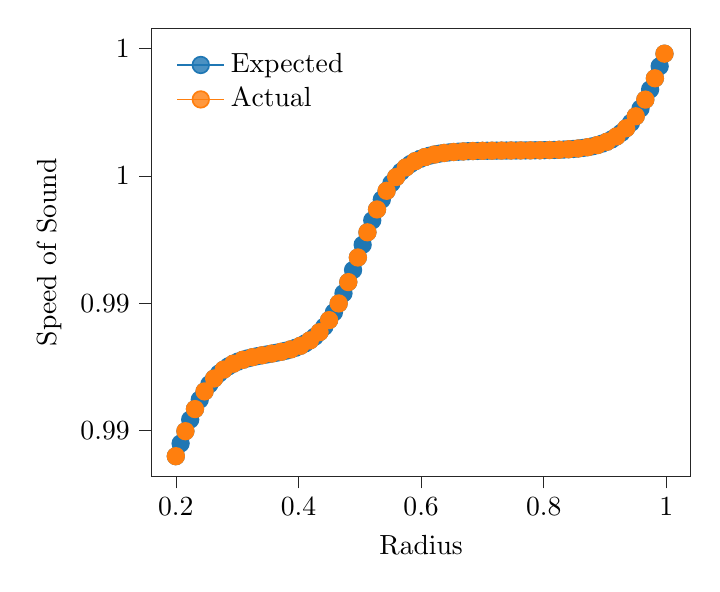
\begin{tikzpicture}

\definecolor{color0}{rgb}{0.12156862745098,0.466666666666667,0.705882352941177}
\definecolor{color1}{rgb}{1,0.498039215686275,0.0549019607843137}

\begin{axis}[
axis line style={white!15!black},
legend cell align={left},
legend style={
  fill opacity=0.8,
  draw opacity=1,
  text opacity=1,
  at={(0.03,0.97)},
  anchor=north west,
  draw=none
},
tick align=outside,
tick pos=left,
x grid style={white!80!black},
xlabel={Radius},
xmin=0.16, xmax=1.04,
xtick style={color=white!15!black},
y grid style={white!80!black},
ylabel={Speed of Sound},
ymin=0.98320056903035, ymax=1.00079997290332,
ytick style={color=white!15!black}
]
\addplot [semithick, color0, mark=*, mark size=3, mark repeat=5, mark options={solid}]
table {%
0.2 0.984000541933667
0.2015625 0.984100548886647
0.203125 0.984200432419622
0.2046875 0.984300068384446
0.20625 0.984399333875707
0.2078125 0.984498107834061
0.209375 0.984596271630271
0.2109375 0.984693709624082
0.2125 0.984790309692462
0.2140625 0.984885963722324
0.215625 0.984980568063398
0.2171875 0.985074023937652
0.21875 0.985166237802302
0.2203125 0.985257121664242
0.221875 0.985346593344428
0.2234375 0.985434576691501
0.225 0.985521001744648
0.2265625 0.985605804846342
0.228125 0.985688928706271
0.2296875 0.985770322418282
0.23125 0.985849941432696
0.2328125 0.985927747486754
0.234375 0.986003708496322
0.2359375 0.986077798412233
0.2375 0.986149997044859
0.2390625 0.986220289860638
0.240625 0.986288667754308
0.2421875 0.986355126800626
0.24375 0.986419667989276
0.2453125 0.986482296946548
0.246875 0.986543023647233
0.2484375 0.986601862119971
0.25 0.986658830149088
0.2515625 0.986713948975696
0.253125 0.98676724300061
0.2546875 0.98681873949133
0.25625 0.986868468295113
0.2578125 0.986916461559873
0.259375 0.986962753464396
0.2609375 0.987007379959106
0.2625 0.987050378518398
0.2640625 0.987091787905317
0.265625 0.987131647949157
0.2671875 0.987169999336396
0.26875 0.98720688341517
0.2703125 0.987242342013376
0.271875 0.987276417270339
0.2734375 0.987309151481869
0.275 0.987340586958444
0.2765625 0.987370765896143
0.278125 0.987399730259926
0.2796875 0.987427521678759
0.28125 0.987454181352077
0.2828125 0.987479749967015
0.284375 0.987504267625839
0.2859375 0.987527773782981
0.2875 0.987550307191088
0.2890625 0.987571905855486
0.290625 0.987592606996474
0.2921875 0.987612447018872
0.29375 0.987631461488276
0.2953125 0.987649685113462
0.296875 0.987667151734442
0.2984375 0.987683894315661
0.3 0.987699944943884
0.3015625 0.987715334830319
0.303125 0.987730094316565
0.3046875 0.987744252883996
0.30625 0.987757839166223
0.3078125 0.987770880964282
0.309375 0.987783405264264
0.3109375 0.987795438257075
0.3125 0.987807005360076
0.3140625 0.987818131240364
0.315625 0.987828839839472
0.3171875 0.987839154399291
0.31875 0.98784909748904
0.3203125 0.987858691033117
0.321875 0.9878679563397
0.3234375 0.987876914129958
0.325 0.987885584567766
0.3265625 0.987893987289837
0.328125 0.98790214143616
0.3296875 0.987910065680699
0.33125 0.987917778262275
0.3328125 0.987925297015572
0.334375 0.987932639402246
0.3359375 0.987939822542074
0.3375 0.987946863244137
0.3390625 0.987953778037998
0.340625 0.987960583204877
0.3421875 0.987967294808789
0.34375 0.98797392872766
0.3453125 0.987980500684408
0.346875 0.987987026277992
0.3484375 0.987993521014427
0.35 0.988000000337782
0.3515625 0.988006479661155
0.353125 0.988012974397646
0.3546875 0.988019499991323
0.35625 0.988026071948201
0.3578125 0.988032705867241
0.359375 0.988039417471358
0.3609375 0.988046222638482
0.3625 0.988053137432628
0.3640625 0.988060178135015
0.365625 0.988067361275209
0.3671875 0.98807470366229
0.36875 0.988082222416037
0.3703125 0.988089934998106
0.371875 0.988097859243185
0.3734375 0.988106013390094
0.375 0.988114416112798
0.3765625 0.988123086551289
0.378125 0.988132044342281
0.3796875 0.988141309649652
0.38125 0.988150903194572
0.3828125 0.98816084628522
0.384375 0.988171160845998
0.3859375 0.988181869446127
0.3875 0.9881929953275
0.3890625 0.988204562431654
0.390625 0.988216595425687
0.3921875 0.988229119726965
0.39375 0.988242161526395
0.3953125 0.988255747810073
0.396875 0.988269906379039
0.3984375 0.988284665866907
0.4 0.988300055755055
0.4015625 0.988316106385087
0.403125 0.988332848968214
0.4046875 0.988350315591207
0.40625 0.988368539218517
0.4078125 0.988387553690159
0.409375 0.988407393714916
0.4109375 0.988428094858389
0.4125 0.988449693525406
0.4140625 0.988472226936272
0.415625 0.988495733096318
0.4171875 0.988520250758199
0.41875 0.988545819376356
0.4203125 0.988572479053063
0.421875 0.988600270475462
0.4234375 0.988629234842998
0.425 0.988659413784646
0.4265625 0.988690849265375
0.428125 0.988723583481276
0.4296875 0.988757658742837
0.43125 0.98879311734588
0.4328125 0.988830001429742
0.434375 0.988868352822332
0.4359375 0.9889082128718
0.4375 0.988949622264638
0.4390625 0.988992620830155
0.440625 0.989037247331411
0.4421875 0.989083539242818
0.44375 0.989131532514817
0.4453125 0.989181261326212
0.446875 0.989232757824935
0.4484375 0.989286051858266
0.45 0.989341170693724
0.4515625 0.989398138732145
0.453125 0.989456977214666
0.4546875 0.989517703925637
0.45625 0.989580332893724
0.4578125 0.989644874093744
0.459375 0.989711333152017
0.4609375 0.989779711058255
0.4625 0.989850003887249
0.4640625 0.989922202533768
0.465625 0.989996292464284
0.4671875 0.990072253489208
0.46875 0.99015005955941
0.4703125 0.990229678590797
0.471875 0.990311072320652
0.4734375 0.99039419619934
0.475 0.990478999320756
0.4765625 0.990565424394636
0.478125 0.990653407763507
0.4796875 0.990742879466609
0.48125 0.99083376335264
0.4828125 0.990925977242617
0.484375 0.991019433143496
0.4859375 0.991114037512562
0.4875 0.991209691571851
0.4890625 0.991306291671168
0.490625 0.991403729697502
0.4921875 0.991501893527903
0.49375 0.991600667522201
0.4953125 0.99169993305125
0.496875 0.991799569055799
0.4984375 0.991899452630537
0.5 0.991999459627421
0.5015625 0.992099465272067
0.503125 0.99219934478671
0.5046875 0.992298974013166
0.50625 0.992398230029186
0.5078125 0.992496991751752
0.509375 0.992595140521059
0.5109375 0.992692560659307
0.5125 0.992789139998857
0.5140625 0.99288477037483
0.515625 0.992979348077864
0.5171875 0.99307277426338
0.51875 0.993164955314424
0.5203125 0.993255803155917
0.521875 0.993345235518834
0.5234375 0.993433176153603
0.525 0.993519554992716
0.5265625 0.993604308263212
0.528125 0.993687378550314
0.5296875 0.993768714814062
0.53125 0.993848272361297
0.5328125 0.993926012775751
0.534375 0.994001903809366
0.5359375 0.99407591923823
0.5375 0.994148038686721
0.5390625 0.99421824742356
0.540625 0.994286536133559
0.5421875 0.994352900668823
0.54375 0.994417341783093
0.5453125 0.994479864852854
0.546875 0.994540479588594
0.5484375 0.994599199739509
0.55 0.994656042794637
0.5515625 0.994711029683234
0.553125 0.994764184476907
0.5546875 0.994815534095789
0.55625 0.994865108020749
0.5578125 0.99491293801338
0.559375 0.99495905784526
0.5609375 0.995003503037712
0.5625 0.995046310613072
0.5640625 0.995087518858254
0.565625 0.995127167101171
0.5671875 0.995165295500434
0.56875 0.99520194484852
0.5703125 0.995237156388507
0.571875 0.995270971644298
0.5734375 0.995303432264168
0.575 0.995334579877347
0.5765625 0.995364455963282
0.578125 0.995393101733155
0.5796875 0.995420558023162
0.58125 0.995446865199025
0.5828125 0.995472063071189
0.584375 0.9954961908201
0.5859375 0.995519286930997
0.5875 0.995541389137587
0.5890625 0.995562534374025
0.590625 0.995582758734604
0.5921875 0.995602097440566
0.59375 0.995620584813474
0.5953125 0.995638254254612
0.596875 0.995655138229866
0.5984375 0.995671268259608
0.6 0.995686674913096
0.6015625 0.995701387806942
0.603125 0.995715435607232
0.6046875 0.995728846034892
0.60625 0.99574164587393
0.6078125 0.995753860982223
0.609375 0.995765516304507
0.6109375 0.995776635887292
0.6125 0.995787242895424
0.6140625 0.995797359630043
0.615625 0.995807007547711
0.6171875 0.995816207280501
0.61875 0.995824978656858
0.6203125 0.995833340723064
0.621875 0.995841311765143
0.6234375 0.995848909331092
0.625 0.995856150253272
0.6265625 0.995863050670899
0.628125 0.995869626052497
0.6296875 0.99587589121825
0.63125 0.995881860362164
0.6328125 0.995887547073985
0.634375 0.995892964360806
0.6359375 0.995898124668321
0.6375 0.995903039901678
0.6390625 0.995907721445908
0.640625 0.995912180185882
0.6421875 0.995916426525794
0.64375 0.995920470408134
0.6453125 0.995924321332153
0.646875 0.995927988371789
0.6484375 0.995931480193072
0.65 0.995934805070983
0.6515625 0.995937970905779
0.653125 0.99594098523878
0.6546875 0.995943855267619
0.65625 0.995946587860976
0.6578125 0.995949189572774
0.659375 0.995951666655872
0.6609375 0.995954025075258
0.6625 0.99595627052074
0.6640625 0.995958408419154
0.665625 0.995960443946116
0.6671875 0.995962382037296
0.66875 0.995964227399259
0.6703125 0.995965984519872
0.671875 0.995967657678284
0.6734375 0.995969250954509
0.675 0.995970768238611
0.6765625 0.995972213239507
0.678125 0.995973589493407
0.6796875 0.995974900371901
0.68125 0.995976149089699
0.6828125 0.995977338712054
0.684375 0.995978472161855
0.6859375 0.995979552226434
0.6875 0.995980581564065
0.6890625 0.995981562710198
0.690625 0.995982498083416
0.6921875 0.995983389991139
0.69375 0.995984240635083
0.6953125 0.995985052116483
0.696875 0.995985826441091
0.6984375 0.99598656552396
0.7 0.995987271194022
0.7015625 0.995987945198473
0.703125 0.995988589206969
0.7046875 0.995989204815643
0.70625 0.995989793550959
0.7078125 0.995990356873398
0.709375 0.995990896180996
0.7109375 0.99599141281273
0.7125 0.99599190805178
0.7140625 0.99599238312864
0.715625 0.995992839224128
0.7171875 0.995993277472259
0.71875 0.995993698963021
0.7203125 0.99599410474504
0.721875 0.99599449582815
0.7234375 0.995994873185871
0.725 0.995995237757798
0.7265625 0.995995590451909
0.728125 0.995995932146805
0.7296875 0.995996263693868
0.73125 0.995996585919359
0.7328125 0.995996899626465
0.734375 0.995997205597271
0.7359375 0.9959975045947
0.7375 0.995997797364393
0.7390625 0.995998084636562
0.740625 0.995998367127788
0.7421875 0.995998645542801
0.74375 0.995998920576223
0.7453125 0.995999192914293
0.746875 0.995999463236562
0.7484375 0.995999732217585
0.75 0.996000000528589
0.7515625 0.996000268839138
0.753125 0.996000537818796
0.7546875 0.996000808138787
0.75625 0.996001080473659
0.7578125 0.996001355502957
0.759375 0.996001633912908
0.7609375 0.996001916398121
0.7625 0.996002203663312
0.7640625 0.996002496425045
0.765625 0.996002795413511
0.7671875 0.996003101374329
0.76875 0.996003415070396
0.7703125 0.996003737283773
0.771875 0.996004068817611
0.7734375 0.996004410498143
0.775 0.996004763176713
0.7765625 0.996005127731883
0.778125 0.996005505071589
0.7796875 0.996005896135382
0.78125 0.996006301896732
0.7828125 0.996006723365422
0.784375 0.996007161590024
0.7859375 0.996007617660467
0.7875 0.996008092710702
0.7890625 0.996008587921481
0.790625 0.996009104523228
0.7921875 0.996009643799046
0.79375 0.996010207087836
0.7953125 0.996010795787547
0.796875 0.996011411358571
0.7984375 0.996012055327279
0.8 0.996012729289704
0.8015625 0.996013434915398
0.803125 0.996014173951444
0.8046875 0.996014948226658
0.80625 0.99601575965597
0.8078125 0.996016610245002
0.809375 0.99601750209485
0.8109375 0.996018437407087
0.8125 0.996019418488979
0.8140625 0.99602044775895
0.815625 0.996021527752279
0.8171875 0.996022661127064
0.81875 0.996023850670446
0.8203125 0.996025099305121
0.821875 0.99602641009613
0.8234375 0.996027786257968
0.825 0.996029231161992
0.8265625 0.996030748344171
0.828125 0.996032341513167
0.8296875 0.996034014558775
0.83125 0.996035771560727
0.8328125 0.996037616797878
0.834375 0.996039554757779
0.8359375 0.996041590146669
0.8375 0.996043727899874
0.8390625 0.996045973192643
0.840625 0.996048331451433
0.8421875 0.996050808365651
0.84375 0.99605340989986
0.8453125 0.996056142306476
0.846875 0.996059012138958
0.8484375 0.99606202626549
0.85 0.996065191883192
0.8515625 0.996068516532841
0.853125 0.996072008114122
0.8546875 0.996075674901416
0.85625 0.996079525560123
0.8578125 0.996083569163517
0.859375 0.996087815210152
0.8609375 0.996092273641784
0.8625 0.996096954861836
0.8640625 0.996101869754369
0.865625 0.996107029703561
0.8671875 0.996112446613664
0.86875 0.99611813292943
0.8703125 0.996124101656964
0.871875 0.996130366384967
0.8734375 0.996136941306354
0.875 0.996143841240155
0.8765625 0.996151081653687
0.878125 0.996158678684891
0.8796875 0.996166649164795
0.88125 0.996175010639986
0.8828125 0.996183781395013
0.884375 0.996192980474604
0.8859375 0.99620262770557
0.8875 0.996212743718267
0.8890625 0.996223349967452
0.890625 0.996234468752366
0.8921875 0.996246123235863
0.89375 0.996258337462352
0.8953125 0.996271136374368
0.896875 0.996284545827466
0.8984375 0.99629859260322
0.9 0.996313304419992
0.9015625 0.996328709941177
0.903125 0.996344838780554
0.9046875 0.996361721504406
0.90625 0.996379389629974
0.9078125 0.996397875619856
0.909375 0.996417212871876
0.9109375 0.996437435703965
0.9125 0.99645857933354
0.9140625 0.996480679850876
0.915625 0.996503774185906
0.9171875 0.996527900067896
0.91875 0.996553095977414
0.9203125 0.996579401090003
0.921875 0.996606855210946
0.9234375 0.996635498700543
0.925 0.996665372389287
0.9265625 0.996696517482366
0.928125 0.996728975452927
0.9296875 0.996762787923574
0.93125 0.996797996535619
0.9328125 0.996834642805644
0.934375 0.99687276796903
0.9359375 0.996912412810164
0.9375 0.996953617479149
0.9390625 0.996996421294959
0.940625 0.997040862535105
0.9421875 0.997086978212043
0.94375 0.997134803836707
0.9453125 0.997184373169752
0.946875 0.997235717961291
0.9484375 0.997288867680121
0.95 0.997343849233688
0.9515625 0.99740068668026
0.953125 0.997459400935069
0.9546875 0.997520009472411
0.95625 0.997582526025983
0.9578125 0.997646960289984
0.959375 0.997713317623768
0.9609375 0.997781598763074
0.9625 0.997851799541075
0.9640625 0.997923910622686
0.965625 0.99799791725571
0.9671875 0.998073799042532
0.96875 0.998151529736121
0.9703125 0.998231077064117
0.971875 0.998312402584702
0.9734375 0.998395461577857
0.975 0.998480202975387
0.9765625 0.998566569332831
0.978125 0.998654496846022
0.9796875 0.998743915414651
0.98125 0.998834748754659
0.9828125 0.998926914560766
0.984375 0.999020324719782
0.9859375 0.99911488557469
0.9875 0.99921049823879
0.9890625 0.999307058958444
0.990625 0.999404459522227
0.9921875 0.999502587713568
0.99375 0.999601327803226
0.9953125 0.999700561077321
0.996875 0.999800166395987
0.9984375 0.999900020777216
1 1
};
\addlegendentry{Expected}
\addplot [semithick, color1, mark=*, mark size=3, mark repeat=10, mark options={solid}]
table {%
0.2 0.984000542019354
0.2015625 0.984100538570465
0.203125 0.984200411755927
0.2046875 0.984300037478986
0.20625 0.984399292884513
0.2078125 0.984498056961819
0.209375 0.984596211128208
0.2109375 0.98469363978739
0.2125 0.984790230857325
0.2140625 0.984885876262573
0.215625 0.98498047238688
0.2171875 0.985073920482345
0.21875 0.985166127032258
0.2203125 0.985257004065404
0.221875 0.985346469420391
0.2234375 0.985434446959279
0.225 0.98552086673049
0.2265625 0.985605665081666
0.228125 0.985688784723747
0.2296875 0.985770174748117
0.23125 0.985849790599148
0.2328125 0.985927594004909
0.234375 0.986003552869154
0.2359375 0.986077641127965
0.2375 0.986149838574637
0.2390625 0.986220130656513
0.240625 0.986288508247539
0.2421875 0.986354967400289
0.24375 0.986419509081172
0.2453125 0.986482138892399
0.246875 0.986542866784147
0.2484375 0.98660170676016
0.25 0.986658676579815
0.2515625 0.986713797459438
0.253125 0.986767093775402
0.2546875 0.986818592771284
0.25625 0.986868324271075
0.2578125 0.98691632040021
0.259375 0.986962615315875
0.2609375 0.987007244947868
0.2625 0.987050246750991
0.2640625 0.987091659469774
0.265625 0.987131522916112
0.2671875 0.987169877760217
0.26875 0.987206765335094
0.2703125 0.987242227454642
0.271875 0.987276306245304
0.2734375 0.987309043991106
0.275 0.987340482991801
0.2765625 0.987370665433774
0.278125 0.987399633273278
0.2796875 0.987427428131517
0.28125 0.987454091201058
0.2828125 0.987479663163019
0.284375 0.987504184114449
0.2859375 0.987527693505313
0.2875 0.98755023008449
0.2890625 0.987571831854191
0.290625 0.9875925360322
0.2921875 0.987612379021383
0.29375 0.987631396385893
0.2953125 0.987649622833532
0.296875 0.987667092203763
0.2984375 0.987683837460875
0.3 0.987699890691827
0.3015625 0.987715283108339
0.303125 0.987730045052807
0.3046875 0.987744206007658
0.30625 0.987757794607782
0.3078125 0.987770838655695
0.309375 0.987783365139148
0.3109375 0.98779540025086
0.3125 0.987806969410141
0.3140625 0.987818097286156
0.315625 0.987828807822605
0.3171875 0.987839124263634
0.31875 0.98784906918079
0.3203125 0.987858664500862
0.321875 0.987867931534466
0.3234375 0.987876891005252
0.325 0.987885563079613
0.3265625 0.987893967396799
0.328125 0.987902123099364
0.3296875 0.987910048863849
0.33125 0.987917762931659
0.3328125 0.987925283140076
0.334375 0.987932626953352
0.3359375 0.987939811493866
0.3375 0.987946853573297
0.3390625 0.987953769723811
0.340625 0.98796057622922
0.3421875 0.987967289156136
0.34375 0.987973924385075
0.3453125 0.987980497641544
0.346875 0.987987024527085
0.3484375 0.987993520550299
0.35 0.988000001157834
0.3515625 0.988006481765371
0.353125 0.98801297778859
0.3546875 0.988019504674139
0.35625 0.988026077930618
0.3578125 0.988032713159569
0.359375 0.988039426086497
0.3609375 0.988046232591919
0.3625 0.988053148742442
0.3640625 0.98806019082188
0.365625 0.988067375362393
0.3671875 0.988074719175661
0.36875 0.988082239384058
0.3703125 0.988089953451836
0.371875 0.988097879216269
0.3734375 0.988106034918762
0.375 0.988114439235851
0.3765625 0.988123111310083
0.378125 0.988132070780705
0.3796875 0.988141337814104
0.38125 0.988150933133922
0.3828125 0.988160878050769
0.384375 0.988171194491426
0.3859375 0.988181905027431
0.3875 0.988193032902921
0.3890625 0.988204602061585
0.390625 0.988216637172577
0.3921875 0.988229163655196
0.39375 0.988242207702146
0.3953125 0.988255796301162
0.396875 0.988269957254748
0.3984375 0.988284719197773
0.4 0.988300111612648
0.4015625 0.988316164841748
0.403125 0.98833291009677
0.4046875 0.988350379464653
0.40625 0.988368605909658
0.4078125 0.988387623271224
0.409375 0.988407466257124
0.4109375 0.988428170431479
0.4125 0.988449772197124
0.4140625 0.988472308771811
0.415625 0.988495818157714
0.4171875 0.988520339103674
0.41875 0.988545911059617
0.4203125 0.988572574122552
0.421875 0.988600368973554
0.4234375 0.988629336805148
0.425 0.988659519238492
0.4265625 0.988690958229793
0.428125 0.988723695965391
0.4296875 0.988757774744993
0.43125 0.988793236852577
0.4328125 0.988830124414544
0.434375 0.988868479244747
0.4359375 0.988908342676152
0.4375 0.988949755378929
0.4390625 0.98899275716494
0.440625 0.989037386778686
0.4421875 0.989083681674941
0.44375 0.989131677783485
0.4453125 0.989181409261496
0.446875 0.989232908234404
0.4484375 0.989286204526211
0.45 0.989341325380513
0.4515625 0.989398295173717
0.453125 0.989457135122194
0.4546875 0.989517862985384
0.45625 0.989580492767111
0.4578125 0.989645034417647
0.459375 0.989711493539319
0.4609375 0.98977987109867
0.4625 0.989850163148432
0.4640625 0.989922360562726
0.465625 0.989996448789093
0.4671875 0.990072407621048
0.46875 0.990150210994911
0.4703125 0.990229826814696
0.471875 0.990311216808754
0.4734375 0.990394336421754
0.475 0.990479134745392
0.4765625 0.990565554490936
0.478125 0.990653532006369
0.4796875 0.990742997340459
0.48125 0.99083387435562
0.4828125 0.990926080890818
0.484375 0.991019528975192
0.4859375 0.991114125092381
0.4875 0.991209770494826
0.4890625 0.991306361566602
0.490625 0.991403790232585
0.4921875 0.991501944411025
0.49375 0.991600708505906
0.4953125 0.991699963934777
0.496875 0.991799589687169
0.4984375 0.991899462908144
0.5 0.991999459501105
0.5015625 0.992099454743644
0.503125 0.992199323909957
0.5046875 0.992298942893246
0.50625 0.992398188821544
0.5078125 0.992496940660486
0.509375 0.992595079796797
0.5109375 0.99269249059664
0.5125 0.992789060933354
0.5140625 0.992884682679702
0.515625 0.992979252160325
0.5171875 0.993072670560762
0.51875 0.993164844290118
0.5203125 0.993255685295191
0.521875 0.99334511132459
0.5234375 0.99343304614214
0.525 0.99351941968955
0.5265625 0.993604168199006
0.528125 0.993687234256956
0.5296875 0.993768566820951
0.53125 0.993848121191855
0.5328125 0.993925858944195
0.534375 0.99400174781777
0.5359375 0.994075761573883
0.5375 0.994147879819793
0.5390625 0.994218087805088
0.540625 0.994286376193745
0.5421875 0.99435274081564
0.54375 0.994417182401192
0.5453125 0.994479706302753
0.546875 0.994540322206146
0.5484375 0.99459904383561
0.55 0.994655888655176
0.5515625 0.994710877569247
0.553125 0.994764034624923
0.5546875 0.994815386718341
0.55625 0.994864963307029
0.5578125 0.994912796130018
0.559375 0.994958918937205
0.5609375 0.995003367229198
0.5625 0.995046178008647
0.5640625 0.995087389543851
0.565625 0.995127041145225
0.5671875 0.995165172955
0.56875 0.99520182575041
0.5703125 0.995237040760414
0.571875 0.995270859495909
0.5734375 0.995303323593251
0.575 0.995334474670805
0.5765625 0.995364354198178
0.578125 0.995393003377691
0.5796875 0.995420463037613
0.58125 0.995446773536632
0.5828125 0.995471974678994
0.584375 0.995496105639743
0.5859375 0.99551920489945
0.5875 0.99554131018785
0.5890625 0.995562458435763
0.590625 0.995582685734742
0.5921875 0.995602027303832
0.59375 0.995620517462904
0.5953125 0.995638189612002
0.596875 0.99565507621619
0.5984375 0.99567120879539
0.6 0.99568661791875
0.6015625 0.995701333203077
0.603125 0.995715383314918
0.6046875 0.995728795975899
0.60625 0.995741597970942
0.6078125 0.995753815159019
0.609375 0.995765472486118
0.6109375 0.995776594000141
0.6125 0.995787202867441
0.6140625 0.995797321390759
0.615625 0.995806971028341
0.6171875 0.995816172414004
0.61875 0.995824945377991
0.6203125 0.995833308968413
0.621875 0.995841281473156
0.6234375 0.995848880442084
0.625 0.995856122709439
0.6265625 0.995863024416314
0.628125 0.995869601033097
0.6296875 0.995875867381824
0.63125 0.995881837658331
0.6328125 0.995887525454166
0.634375 0.995892943778198
0.6359375 0.995898105077859
0.6375 0.995903021260004
0.6390625 0.995907703711326
0.640625 0.995912163318324
0.6421875 0.995916410486774
0.64375 0.995920455160706
0.6453125 0.995924306840866
0.646875 0.995927974602643
0.6484375 0.995931467113475
0.65 0.995934792649703
0.6515625 0.9959379591129
0.653125 0.995940974045658
0.6546875 0.995943844646839
0.65625 0.995946577786306
0.6578125 0.995949180019123
0.659375 0.99595165759925
0.6609375 0.995954016492733
0.6625 0.995956262390396
0.6640625 0.995958400720057
0.665625 0.995960436658271
0.6671875 0.99596237514161
0.66875 0.995964220877508
0.6703125 0.995965978354663
0.671875 0.995967651853024
0.6734375 0.99596924545337
0.675 0.995970763046498
0.6765625 0.99597220834203
0.678125 0.995973584876848
0.6796875 0.995974896023187
0.68125 0.995976144996378
0.6828125 0.995977334862262
0.684375 0.995978468544298
0.6859375 0.995979548830358
0.6875 0.995980578379236
0.6890625 0.995981559726879
0.690625 0.995982495292344
0.6921875 0.995983387383507
0.69375 0.995984238202519
0.6953125 0.995985049851032
0.696875 0.995985824335194
0.6984375 0.995986563570442
0.7 0.995987269386074
0.7015625 0.995987943529633
0.703125 0.995988587671111
0.7046875 0.995989203406963
0.70625 0.99598979226396
0.7078125 0.995990355702877
0.709375 0.995990895122031
0.7109375 0.995991411860674
0.7125 0.995991907202242
0.7140625 0.995992382377482
0.715625 0.99599283856745
0.7171875 0.995993276906392
0.71875 0.99599369848452
0.7203125 0.995994104350672
0.721875 0.99599449551489
0.7234375 0.995994872950893
0.725 0.995995237598466
0.7265625 0.995995590365778
0.728125 0.995995932131606
0.7296875 0.995996263747507
0.73125 0.995996586039915
0.7328125 0.995996899812179
0.734375 0.995997205846547
0.7359375 0.995997504906098
0.7375 0.995997797736628
0.7390625 0.995998085068498
0.740625 0.995998367618437
0.7421875 0.995998646091321
0.74375 0.995998921181916
0.7453125 0.995999193576601
0.746875 0.99599946395507
0.7484375 0.995999732992015
0.75 0.996000001358802
0.7515625 0.996000269725134
0.753125 0.996000538760714
0.7546875 0.996000809136904
0.75625 0.996001081528391
0.7578125 0.99600135661486
0.759375 0.99600163508268
0.7609375 0.996001917626605
0.7625 0.996002204951495
0.7640625 0.996002497774063
0.765625 0.996002796824648
0.7671875 0.996003102849025
0.76875 0.996003416610248
0.7703125 0.996003738890537
0.771875 0.996004070493211
0.7734375 0.99600441224467
0.775 0.996004764996435
0.7765625 0.996005129627247
0.778125 0.996005507045229
0.7796875 0.996005898190124
0.78125 0.996006304035602
0.7828125 0.996006725591651
0.784375 0.996007163907057
0.7859375 0.996007620071971
0.7875 0.996008095220578
0.7890625 0.996008590533865
0.790625 0.99600910724251
0.7921875 0.996009646629875
0.79375 0.99601021003513
0.7953125 0.996010798856509
0.796875 0.996011414554698
0.7984375 0.996012058656374
0.8 0.996012732757891
0.8015625 0.996013438529137
0.803125 0.996014177717544
0.8046875 0.996014952152294
0.80625 0.996015763748697
0.8078125 0.996016614512774
0.809375 0.996017506546037
0.8109375 0.996018442050494
0.8125 0.996019423333868
0.8140625 0.996020452815054
0.815625 0.996021533029831
0.8171875 0.996022666636814
0.81875 0.996023856423687
0.8203125 0.996025105313711
0.821875 0.996026416372521
0.8234375 0.996027792815226
0.825 0.996029238013831
0.8265625 0.996030755504977
0.828125 0.99603234899803
0.8296875 0.996034022383518
0.83125 0.996035779741937
0.8328125 0.996037625352941
0.834375 0.996039563704913
0.8359375 0.996041599504958
0.8375 0.996043737689303
0.8390625 0.99604598343414
0.840625 0.996048342166902
0.8421875 0.996050819578012
0.84375 0.996053421633092
0.8453125 0.996056154585657
0.846875 0.996059024990304
0.8484375 0.996062039716402
0.85 0.996065205962296
0.8515625 0.996068531270032
0.853125 0.996072023540612
0.8546875 0.996075691049775
0.85625 0.996079542464325
0.8578125 0.996083586858985
0.859375 0.996087833733802
0.8609375 0.996092293032069
0.8625 0.996096975158789
0.8640625 0.996101890999645
0.865625 0.996107051940475
0.8671875 0.996112469887234
0.86875 0.996118157286407
0.8703125 0.996124127145869
0.871875 0.99613039305612
0.8734375 0.996136969211897
0.875 0.996143870434077
0.8765625 0.996151112191834
0.878125 0.996158710624979
0.8796875 0.996166682566409
0.88125 0.996175045564575
0.8828125 0.996183817905873
0.884375 0.996193018636852
0.8859375 0.996202667586109
0.8875 0.996212785385732
0.8890625 0.996223393492147
0.890625 0.996234514206185
0.8921875 0.996246170692186
0.89375 0.996258386995937
0.8953125 0.996271188061206
0.896875 0.996284599744623
0.8984375 0.996298648828654
0.9 0.996313363032339
0.9015625 0.996328771019508
0.903125 0.99634490240411
0.9046875 0.996361787752286
0.90625 0.996379458580801
0.9078125 0.996397947351397
0.909375 0.996417287460625
0.9109375 0.996437513224683
0.9125 0.996458659858756
0.9140625 0.996480763450336
0.915625 0.996503860925981
0.9171875 0.996527990010936
0.91875 0.996553189181057
0.9203125 0.996579497606432
0.921875 0.996606955086097
0.9234375 0.996635601973261
0.925 0.996665479090439
0.9265625 0.9966966276339
0.928125 0.996729089066892
0.9296875 0.9967629050011
0.93125 0.996798117065855
0.9328125 0.996834766764676
0.934375 0.996872895318767
0.9359375 0.996912543497216
0.9375 0.996953751433694
0.9390625 0.996996558429622
0.940625 0.997041002743852
0.9421875 0.997087121369108
0.94375 0.997134949795571
0.9453125 0.997184521762187
0.946875 0.997235868996483
0.9484375 0.997289020943902
0.95 0.997344004487888
0.9515625 0.997400843662211
0.953125 0.997459559357272
0.9546875 0.997520169022392
0.95625 0.997582686366363
0.9578125 0.997647121058781
0.959375 0.997713478434953
0.9609375 0.997781759207394
0.9625 0.997851959187171
0.9640625 0.997924069018498
0.965625 0.997998073930204
0.9671875 0.998073953507733
0.96875 0.998151681489463
0.9703125 0.998231225591102
0.971875 0.99831254736186
0.9734375 0.998395602075987
0.975 0.998480338663054
0.9765625 0.998566699680098
0.978125 0.998654621328378
0.9796875 0.998744033517082
0.98125 0.998834859975838
0.9828125 0.998927018417289
0.984375 0.999020420750399
0.9859375 0.999114973344484
0.9875 0.999210577343224
0.9890625 0.999307129027227
0.990625 0.999404520222934
0.9921875 0.999502638754955
0.99375 0.999601368938184
0.9953125 0.999700592105417
0.996875 0.999800187165552
0.9984375 0.999900031186939
1 1
};
\addlegendentry{Actual}
\end{axis}

\end{tikzpicture}
}
     \end{center}
     \caption{Speed of Sound from Integrating the Tangential Mach Number}
 \end{figure}

% \begin{figure}
%     \begin{center}
%         \scalebox{0.75}{\begin{tikzpicture}[gnuplot]
%% generated with GNUPLOT 5.2p8 (Lua 5.3; terminal rev. Nov 2018, script rev. 108)
%% Wed 01 Sep 2021 01:14:21 AM EDT
\path (0.000,0.000) rectangle (12.500,8.750);
\gpcolor{color=gp lt color axes}
\gpsetlinetype{gp lt axes}
\gpsetdashtype{gp dt axes}
\gpsetlinewidth{0.50}
\draw[gp path] (2.240,0.985)--(11.947,0.985);
\gpcolor{color=gp lt color border}
\gpsetlinetype{gp lt border}
\gpsetdashtype{gp dt solid}
\gpsetlinewidth{1.00}
\draw[gp path] (2.240,0.985)--(2.420,0.985);
\draw[gp path] (11.947,0.985)--(11.767,0.985);
\node[gp node right] at (2.056,0.985) {$0$};
\gpcolor{color=gp lt color axes}
\gpsetlinetype{gp lt axes}
\gpsetdashtype{gp dt axes}
\gpsetlinewidth{0.50}
\draw[gp path] (2.240,2.050)--(11.947,2.050);
\gpcolor{color=gp lt color border}
\gpsetlinetype{gp lt border}
\gpsetdashtype{gp dt solid}
\gpsetlinewidth{1.00}
\draw[gp path] (2.240,2.050)--(2.420,2.050);
\draw[gp path] (11.947,2.050)--(11.767,2.050);
\node[gp node right] at (2.056,2.050) {$2\times10^{-9}$};
\gpcolor{color=gp lt color axes}
\gpsetlinetype{gp lt axes}
\gpsetdashtype{gp dt axes}
\gpsetlinewidth{0.50}
\draw[gp path] (2.240,3.115)--(11.947,3.115);
\gpcolor{color=gp lt color border}
\gpsetlinetype{gp lt border}
\gpsetdashtype{gp dt solid}
\gpsetlinewidth{1.00}
\draw[gp path] (2.240,3.115)--(2.420,3.115);
\draw[gp path] (11.947,3.115)--(11.767,3.115);
\node[gp node right] at (2.056,3.115) {$4\times10^{-9}$};
\gpcolor{color=gp lt color axes}
\gpsetlinetype{gp lt axes}
\gpsetdashtype{gp dt axes}
\gpsetlinewidth{0.50}
\draw[gp path] (2.240,4.180)--(11.947,4.180);
\gpcolor{color=gp lt color border}
\gpsetlinetype{gp lt border}
\gpsetdashtype{gp dt solid}
\gpsetlinewidth{1.00}
\draw[gp path] (2.240,4.180)--(2.420,4.180);
\draw[gp path] (11.947,4.180)--(11.767,4.180);
\node[gp node right] at (2.056,4.180) {$6\times10^{-9}$};
\gpcolor{color=gp lt color axes}
\gpsetlinetype{gp lt axes}
\gpsetdashtype{gp dt axes}
\gpsetlinewidth{0.50}
\draw[gp path] (2.240,5.246)--(11.947,5.246);
\gpcolor{color=gp lt color border}
\gpsetlinetype{gp lt border}
\gpsetdashtype{gp dt solid}
\gpsetlinewidth{1.00}
\draw[gp path] (2.240,5.246)--(2.420,5.246);
\draw[gp path] (11.947,5.246)--(11.767,5.246);
\node[gp node right] at (2.056,5.246) {$8\times10^{-9}$};
\gpcolor{color=gp lt color axes}
\gpsetlinetype{gp lt axes}
\gpsetdashtype{gp dt axes}
\gpsetlinewidth{0.50}
\draw[gp path] (2.240,6.311)--(11.947,6.311);
\gpcolor{color=gp lt color border}
\gpsetlinetype{gp lt border}
\gpsetdashtype{gp dt solid}
\gpsetlinewidth{1.00}
\draw[gp path] (2.240,6.311)--(2.420,6.311);
\draw[gp path] (11.947,6.311)--(11.767,6.311);
\node[gp node right] at (2.056,6.311) {$1\times10^{-8}$};
\gpcolor{color=gp lt color axes}
\gpsetlinetype{gp lt axes}
\gpsetdashtype{gp dt axes}
\gpsetlinewidth{0.50}
\draw[gp path] (2.240,7.376)--(11.947,7.376);
\gpcolor{color=gp lt color border}
\gpsetlinetype{gp lt border}
\gpsetdashtype{gp dt solid}
\gpsetlinewidth{1.00}
\draw[gp path] (2.240,7.376)--(2.420,7.376);
\draw[gp path] (11.947,7.376)--(11.767,7.376);
\node[gp node right] at (2.056,7.376) {$1.2\times10^{-8}$};
\gpcolor{color=gp lt color axes}
\gpsetlinetype{gp lt axes}
\gpsetdashtype{gp dt axes}
\gpsetlinewidth{0.50}
\draw[gp path] (2.240,8.441)--(11.947,8.441);
\gpcolor{color=gp lt color border}
\gpsetlinetype{gp lt border}
\gpsetdashtype{gp dt solid}
\gpsetlinewidth{1.00}
\draw[gp path] (2.240,8.441)--(2.420,8.441);
\draw[gp path] (11.947,8.441)--(11.767,8.441);
\node[gp node right] at (2.056,8.441) {$1.4\times10^{-8}$};
\gpcolor{color=gp lt color axes}
\gpsetlinetype{gp lt axes}
\gpsetdashtype{gp dt axes}
\gpsetlinewidth{0.50}
\draw[gp path] (2.240,0.985)--(2.240,8.441);
\gpcolor{color=gp lt color border}
\gpsetlinetype{gp lt border}
\gpsetdashtype{gp dt solid}
\gpsetlinewidth{1.00}
\draw[gp path] (2.240,0.985)--(2.240,1.165);
\draw[gp path] (2.240,8.441)--(2.240,8.261);
\node[gp node center] at (2.240,0.677) {$0.2$};
\gpcolor{color=gp lt color axes}
\gpsetlinetype{gp lt axes}
\gpsetdashtype{gp dt axes}
\gpsetlinewidth{0.50}
\draw[gp path] (3.453,0.985)--(3.453,8.441);
\gpcolor{color=gp lt color border}
\gpsetlinetype{gp lt border}
\gpsetdashtype{gp dt solid}
\gpsetlinewidth{1.00}
\draw[gp path] (3.453,0.985)--(3.453,1.165);
\draw[gp path] (3.453,8.441)--(3.453,8.261);
\node[gp node center] at (3.453,0.677) {$0.3$};
\gpcolor{color=gp lt color axes}
\gpsetlinetype{gp lt axes}
\gpsetdashtype{gp dt axes}
\gpsetlinewidth{0.50}
\draw[gp path] (4.667,0.985)--(4.667,7.953);
\draw[gp path] (4.667,8.261)--(4.667,8.441);
\gpcolor{color=gp lt color border}
\gpsetlinetype{gp lt border}
\gpsetdashtype{gp dt solid}
\gpsetlinewidth{1.00}
\draw[gp path] (4.667,0.985)--(4.667,1.165);
\draw[gp path] (4.667,8.441)--(4.667,8.261);
\node[gp node center] at (4.667,0.677) {$0.4$};
\gpcolor{color=gp lt color axes}
\gpsetlinetype{gp lt axes}
\gpsetdashtype{gp dt axes}
\gpsetlinewidth{0.50}
\draw[gp path] (5.880,0.985)--(5.880,7.953);
\draw[gp path] (5.880,8.261)--(5.880,8.441);
\gpcolor{color=gp lt color border}
\gpsetlinetype{gp lt border}
\gpsetdashtype{gp dt solid}
\gpsetlinewidth{1.00}
\draw[gp path] (5.880,0.985)--(5.880,1.165);
\draw[gp path] (5.880,8.441)--(5.880,8.261);
\node[gp node center] at (5.880,0.677) {$0.5$};
\gpcolor{color=gp lt color axes}
\gpsetlinetype{gp lt axes}
\gpsetdashtype{gp dt axes}
\gpsetlinewidth{0.50}
\draw[gp path] (7.094,0.985)--(7.094,7.953);
\draw[gp path] (7.094,8.261)--(7.094,8.441);
\gpcolor{color=gp lt color border}
\gpsetlinetype{gp lt border}
\gpsetdashtype{gp dt solid}
\gpsetlinewidth{1.00}
\draw[gp path] (7.094,0.985)--(7.094,1.165);
\draw[gp path] (7.094,8.441)--(7.094,8.261);
\node[gp node center] at (7.094,0.677) {$0.6$};
\gpcolor{color=gp lt color axes}
\gpsetlinetype{gp lt axes}
\gpsetdashtype{gp dt axes}
\gpsetlinewidth{0.50}
\draw[gp path] (8.307,0.985)--(8.307,7.953);
\draw[gp path] (8.307,8.261)--(8.307,8.441);
\gpcolor{color=gp lt color border}
\gpsetlinetype{gp lt border}
\gpsetdashtype{gp dt solid}
\gpsetlinewidth{1.00}
\draw[gp path] (8.307,0.985)--(8.307,1.165);
\draw[gp path] (8.307,8.441)--(8.307,8.261);
\node[gp node center] at (8.307,0.677) {$0.7$};
\gpcolor{color=gp lt color axes}
\gpsetlinetype{gp lt axes}
\gpsetdashtype{gp dt axes}
\gpsetlinewidth{0.50}
\draw[gp path] (9.520,0.985)--(9.520,7.953);
\draw[gp path] (9.520,8.261)--(9.520,8.441);
\gpcolor{color=gp lt color border}
\gpsetlinetype{gp lt border}
\gpsetdashtype{gp dt solid}
\gpsetlinewidth{1.00}
\draw[gp path] (9.520,0.985)--(9.520,1.165);
\draw[gp path] (9.520,8.441)--(9.520,8.261);
\node[gp node center] at (9.520,0.677) {$0.8$};
\gpcolor{color=gp lt color axes}
\gpsetlinetype{gp lt axes}
\gpsetdashtype{gp dt axes}
\gpsetlinewidth{0.50}
\draw[gp path] (10.734,0.985)--(10.734,7.953);
\draw[gp path] (10.734,8.261)--(10.734,8.441);
\gpcolor{color=gp lt color border}
\gpsetlinetype{gp lt border}
\gpsetdashtype{gp dt solid}
\gpsetlinewidth{1.00}
\draw[gp path] (10.734,0.985)--(10.734,1.165);
\draw[gp path] (10.734,8.441)--(10.734,8.261);
\node[gp node center] at (10.734,0.677) {$0.9$};
\gpcolor{color=gp lt color axes}
\gpsetlinetype{gp lt axes}
\gpsetdashtype{gp dt axes}
\gpsetlinewidth{0.50}
\draw[gp path] (11.947,0.985)--(11.947,8.441);
\gpcolor{color=gp lt color border}
\gpsetlinetype{gp lt border}
\gpsetdashtype{gp dt solid}
\gpsetlinewidth{1.00}
\draw[gp path] (11.947,0.985)--(11.947,1.165);
\draw[gp path] (11.947,8.441)--(11.947,8.261);
\node[gp node center] at (11.947,0.677) {$1$};
\draw[gp path] (2.240,8.441)--(2.240,0.985)--(11.947,0.985)--(11.947,8.441)--cycle;
\node[gp node center,rotate=-270] at (0.292,4.713) {Sound Speed Error};
\node[gp node center] at (7.093,0.215) {Radius [-]};
\node[gp node right] at (10.479,8.107) {"../SoundSpeedError.dat" using 1:2};
\gpcolor{rgb color={0.165,0.518,0.647}}
\draw[gp path] (10.663,8.107)--(11.579,8.107);
\draw[gp path] (2.240,8.253)--(2.259,8.253)--(2.278,8.253)--(2.297,8.253)--(2.316,8.252)%
  --(2.335,8.252)--(2.354,8.251)--(2.373,8.251)--(2.392,8.250)--(2.411,8.249)--(2.430,8.249)%
  --(2.449,8.248)--(2.468,8.247)--(2.486,8.246)--(2.505,8.246)--(2.524,8.245)--(2.543,8.244)%
  --(2.562,8.243)--(2.581,8.242)--(2.600,8.240)--(2.619,8.239)--(2.638,8.238)--(2.657,8.237)%
  --(2.676,8.235)--(2.695,8.234)--(2.714,8.233)--(2.733,8.231)--(2.752,8.230)--(2.771,8.228)%
  --(2.790,8.226)--(2.809,8.225)--(2.828,8.223)--(2.847,8.221)--(2.866,8.219)--(2.885,8.218)%
  --(2.904,8.216)--(2.923,8.214)--(2.941,8.212)--(2.960,8.209)--(2.979,8.207)--(2.998,8.205)%
  --(3.017,8.203)--(3.036,8.201)--(3.055,8.198)--(3.074,8.196)--(3.093,8.193)--(3.112,8.191)%
  --(3.131,8.188)--(3.150,8.186)--(3.169,8.183)--(3.188,8.180)--(3.207,8.178)--(3.226,8.175)%
  --(3.245,8.172)--(3.264,8.169)--(3.283,8.166)--(3.302,8.163)--(3.321,8.160)--(3.340,8.157)%
  --(3.359,8.153)--(3.378,8.150)--(3.396,8.147)--(3.415,8.143)--(3.434,8.140)--(3.453,8.136)%
  --(3.472,8.133)--(3.491,8.129)--(3.510,8.126)--(3.529,8.122)--(3.548,8.118)--(3.567,8.114)%
  --(3.586,8.110)--(3.605,8.106)--(3.624,8.102)--(3.643,8.098)--(3.662,8.094)--(3.681,8.090)%
  --(3.700,8.086)--(3.719,8.082)--(3.738,8.077)--(3.757,8.073)--(3.776,8.068)--(3.795,8.064)%
  --(3.814,8.059)--(3.833,8.055)--(3.852,8.050)--(3.870,8.045)--(3.889,8.040)--(3.908,8.035)%
  --(3.927,8.030)--(3.946,8.026)--(3.965,8.020)--(3.984,8.015)--(4.003,8.010)--(4.022,8.005)%
  --(4.041,8.000)--(4.060,7.994)--(4.079,7.989)--(4.098,7.983)--(4.117,7.978)--(4.136,7.972)%
  --(4.155,7.967)--(4.174,7.961)--(4.193,7.955)--(4.212,7.949)--(4.231,7.944)--(4.250,7.938)%
  --(4.269,7.932)--(4.288,7.925)--(4.307,7.919)--(4.325,7.913)--(4.344,7.907)--(4.363,7.901)%
  --(4.382,7.894)--(4.401,7.888)--(4.420,7.881)--(4.439,7.875)--(4.458,7.868)--(4.477,7.861)%
  --(4.496,7.855)--(4.515,7.848)--(4.534,7.841)--(4.553,7.834)--(4.572,7.827)--(4.591,7.820)%
  --(4.610,7.813)--(4.629,7.806)--(4.648,7.798)--(4.667,7.791)--(4.686,7.784)--(4.705,7.776)%
  --(4.724,7.769)--(4.743,7.761)--(4.762,7.754)--(4.781,7.746)--(4.799,7.738)--(4.818,7.731)%
  --(4.837,7.723)--(4.856,7.715)--(4.875,7.707)--(4.894,7.699)--(4.913,7.691)--(4.932,7.682)%
  --(4.951,7.674)--(4.970,7.666)--(4.989,7.657)--(5.008,7.649)--(5.027,7.640)--(5.046,7.632)%
  --(5.065,7.623)--(5.084,7.615)--(5.103,7.606)--(5.122,7.597)--(5.141,7.588)--(5.160,7.579)%
  --(5.179,7.570)--(5.198,7.561)--(5.217,7.552)--(5.236,7.543)--(5.254,7.533)--(5.273,7.524)%
  --(5.292,7.515)--(5.311,7.505)--(5.330,7.496)--(5.349,7.486)--(5.368,7.476)--(5.387,7.467)%
  --(5.406,7.457)--(5.425,7.447)--(5.444,7.437)--(5.463,7.427)--(5.482,7.417)--(5.501,7.407)%
  --(5.520,7.397)--(5.539,7.387)--(5.558,7.376)--(5.577,7.366)--(5.596,7.356)--(5.615,7.345)%
  --(5.634,7.334)--(5.653,7.324)--(5.672,7.313)--(5.691,7.302)--(5.709,7.292)--(5.728,7.281)%
  --(5.747,7.270)--(5.766,7.259)--(5.785,7.248)--(5.804,7.237)--(5.823,7.225)--(5.842,7.214)%
  --(5.861,7.203)--(5.880,7.191)--(5.899,7.180)--(5.918,7.168)--(5.937,7.157)--(5.956,7.145)%
  --(5.975,7.133)--(5.994,7.122)--(6.013,7.110)--(6.032,7.098)--(6.051,7.086)--(6.070,7.074)%
  --(6.089,7.062)--(6.108,7.049)--(6.127,7.037)--(6.146,7.025)--(6.165,7.013)--(6.183,7.000)%
  --(6.202,6.988)--(6.221,6.975)--(6.240,6.962)--(6.259,6.950)--(6.278,6.937)--(6.297,6.924)%
  --(6.316,6.911)--(6.335,6.898)--(6.354,6.885)--(6.373,6.872)--(6.392,6.859)--(6.411,6.846)%
  --(6.430,6.833)--(6.449,6.819)--(6.468,6.806)--(6.487,6.792)--(6.506,6.779)--(6.525,6.765)%
  --(6.544,6.752)--(6.563,6.738)--(6.582,6.724)--(6.601,6.710)--(6.620,6.697)--(6.638,6.683)%
  --(6.657,6.669)--(6.676,6.654)--(6.695,6.640)--(6.714,6.626)--(6.733,6.612)--(6.752,6.597)%
  --(6.771,6.583)--(6.790,6.569)--(6.809,6.554)--(6.828,6.540)--(6.847,6.525)--(6.866,6.510)%
  --(6.885,6.495)--(6.904,6.481)--(6.923,6.466)--(6.942,6.451)--(6.961,6.436)--(6.980,6.421)%
  --(6.999,6.405)--(7.018,6.390)--(7.037,6.375)--(7.056,6.360)--(7.075,6.344)--(7.094,6.329)%
  --(7.112,6.313)--(7.131,6.298)--(7.150,6.282)--(7.169,6.266)--(7.188,6.251)--(7.207,6.235)%
  --(7.226,6.219)--(7.245,6.203)--(7.264,6.187)--(7.283,6.171)--(7.302,6.155)--(7.321,6.139)%
  --(7.340,6.123)--(7.359,6.106)--(7.378,6.090)--(7.397,6.074)--(7.416,6.057)--(7.435,6.041)%
  --(7.454,6.024)--(7.473,6.007)--(7.492,5.991)--(7.511,5.974)--(7.530,5.957)--(7.549,5.940)%
  --(7.567,5.923)--(7.586,5.906)--(7.605,5.889)--(7.624,5.872)--(7.643,5.855)--(7.662,5.838)%
  --(7.681,5.821)--(7.700,5.803)--(7.719,5.786)--(7.738,5.769)--(7.757,5.751)--(7.776,5.733)%
  --(7.795,5.716)--(7.814,5.698)--(7.833,5.681)--(7.852,5.663)--(7.871,5.645)--(7.890,5.627)%
  --(7.909,5.609)--(7.928,5.591)--(7.947,5.573)--(7.966,5.555)--(7.985,5.537)--(8.004,5.519)%
  --(8.022,5.500)--(8.041,5.482)--(8.060,5.464)--(8.079,5.445)--(8.098,5.427)--(8.117,5.408)%
  --(8.136,5.390)--(8.155,5.371)--(8.174,5.353)--(8.193,5.334)--(8.212,5.315)--(8.231,5.296)%
  --(8.250,5.277)--(8.269,5.259)--(8.288,5.240)--(8.307,5.221)--(8.326,5.201)--(8.345,5.182)%
  --(8.364,5.163)--(8.383,5.144)--(8.402,5.125)--(8.421,5.105)--(8.440,5.086)--(8.459,5.067)%
  --(8.478,5.047)--(8.496,5.028)--(8.515,5.008)--(8.534,4.989)--(8.553,4.969)--(8.572,4.949)%
  --(8.591,4.929)--(8.610,4.910)--(8.629,4.890)--(8.648,4.870)--(8.667,4.850)--(8.686,4.830)%
  --(8.705,4.810)--(8.724,4.790)--(8.743,4.770)--(8.762,4.750)--(8.781,4.730)--(8.800,4.709)%
  --(8.819,4.689)--(8.838,4.669)--(8.857,4.648)--(8.876,4.628)--(8.895,4.607)--(8.914,4.587)%
  --(8.933,4.566)--(8.951,4.546)--(8.970,4.525)--(8.989,4.505)--(9.008,4.484)--(9.027,4.463)%
  --(9.046,4.442)--(9.065,4.422)--(9.084,4.401)--(9.103,4.380)--(9.122,4.359)--(9.141,4.338)%
  --(9.160,4.317)--(9.179,4.296)--(9.198,4.275)--(9.217,4.254)--(9.236,4.232)--(9.255,4.211)%
  --(9.274,4.190)--(9.293,4.169)--(9.312,4.147)--(9.331,4.126)--(9.350,4.105)--(9.369,4.083)%
  --(9.388,4.062)--(9.406,4.040)--(9.425,4.019)--(9.444,3.997)--(9.463,3.976)--(9.482,3.954)%
  --(9.501,3.932)--(9.520,3.911)--(9.539,3.889)--(9.558,3.867)--(9.577,3.845)--(9.596,3.824)%
  --(9.615,3.802)--(9.634,3.780)--(9.653,3.758)--(9.672,3.736)--(9.691,3.714)--(9.710,3.692)%
  --(9.729,3.670)--(9.748,3.648)--(9.767,3.626)--(9.786,3.604)--(9.805,3.582)--(9.824,3.559)%
  --(9.843,3.537)--(9.862,3.515)--(9.880,3.493)--(9.899,3.470)--(9.918,3.448)--(9.937,3.426)%
  --(9.956,3.403)--(9.975,3.381)--(9.994,3.359)--(10.013,3.336)--(10.032,3.314)--(10.051,3.291)%
  --(10.070,3.269)--(10.089,3.246)--(10.108,3.224)--(10.127,3.201)--(10.146,3.178)--(10.165,3.156)%
  --(10.184,3.133)--(10.203,3.111)--(10.222,3.088)--(10.241,3.065)--(10.260,3.042)--(10.279,3.020)%
  --(10.298,2.997)--(10.317,2.974)--(10.335,2.951)--(10.354,2.929)--(10.373,2.906)--(10.392,2.883)%
  --(10.411,2.860)--(10.430,2.837)--(10.449,2.814)--(10.468,2.791)--(10.487,2.768)--(10.506,2.745)%
  --(10.525,2.723)--(10.544,2.700)--(10.563,2.677)--(10.582,2.654)--(10.601,2.631)--(10.620,2.607)%
  --(10.639,2.584)--(10.658,2.561)--(10.677,2.538)--(10.696,2.515)--(10.715,2.492)--(10.734,2.469)%
  --(10.753,2.446)--(10.772,2.423)--(10.791,2.400)--(10.809,2.377)--(10.828,2.353)--(10.847,2.330)%
  --(10.866,2.307)--(10.885,2.284)--(10.904,2.261)--(10.923,2.238)--(10.942,2.214)--(10.961,2.191)%
  --(10.980,2.168)--(10.999,2.145)--(11.018,2.121)--(11.037,2.098)--(11.056,2.075)--(11.075,2.052)%
  --(11.094,2.029)--(11.113,2.005)--(11.132,1.982)--(11.151,1.959)--(11.170,1.936)--(11.189,1.912)%
  --(11.208,1.889)--(11.227,1.866)--(11.246,1.843)--(11.264,1.819)--(11.283,1.796)--(11.302,1.773)%
  --(11.321,1.750)--(11.340,1.726)--(11.359,1.703)--(11.378,1.680)--(11.397,1.657)--(11.416,1.633)%
  --(11.435,1.610)--(11.454,1.587)--(11.473,1.564)--(11.492,1.540)--(11.511,1.517)--(11.530,1.494)%
  --(11.549,1.471)--(11.568,1.447)--(11.587,1.424)--(11.606,1.401)--(11.625,1.378)--(11.644,1.355)%
  --(11.663,1.332)--(11.682,1.308)--(11.701,1.285)--(11.719,1.262)--(11.738,1.239)--(11.757,1.216)%
  --(11.776,1.193)--(11.795,1.170)--(11.814,1.146)--(11.833,1.123)--(11.852,1.100)--(11.871,1.077)%
  --(11.890,1.054)--(11.909,1.031)--(11.928,1.008)--(11.947,0.985);
\gpsetpointsize{4.00}
\gppoint{gp mark 1}{(2.240,8.253)}
\gppoint{gp mark 1}{(2.430,8.249)}
\gppoint{gp mark 1}{(2.619,8.239)}
\gppoint{gp mark 1}{(2.809,8.225)}
\gppoint{gp mark 1}{(2.998,8.205)}
\gppoint{gp mark 1}{(3.188,8.180)}
\gppoint{gp mark 1}{(3.378,8.150)}
\gppoint{gp mark 1}{(3.567,8.114)}
\gppoint{gp mark 1}{(3.757,8.073)}
\gppoint{gp mark 1}{(3.946,8.026)}
\gppoint{gp mark 1}{(4.136,7.972)}
\gppoint{gp mark 1}{(4.325,7.913)}
\gppoint{gp mark 1}{(4.515,7.848)}
\gppoint{gp mark 1}{(4.705,7.776)}
\gppoint{gp mark 1}{(4.894,7.699)}
\gppoint{gp mark 1}{(5.084,7.615)}
\gppoint{gp mark 1}{(5.273,7.524)}
\gppoint{gp mark 1}{(5.463,7.427)}
\gppoint{gp mark 1}{(5.653,7.324)}
\gppoint{gp mark 1}{(5.842,7.214)}
\gppoint{gp mark 1}{(6.032,7.098)}
\gppoint{gp mark 1}{(6.221,6.975)}
\gppoint{gp mark 1}{(6.411,6.846)}
\gppoint{gp mark 1}{(6.601,6.710)}
\gppoint{gp mark 1}{(6.790,6.569)}
\gppoint{gp mark 1}{(6.980,6.421)}
\gppoint{gp mark 1}{(7.169,6.266)}
\gppoint{gp mark 1}{(7.359,6.106)}
\gppoint{gp mark 1}{(7.549,5.940)}
\gppoint{gp mark 1}{(7.738,5.769)}
\gppoint{gp mark 1}{(7.928,5.591)}
\gppoint{gp mark 1}{(8.117,5.408)}
\gppoint{gp mark 1}{(8.307,5.221)}
\gppoint{gp mark 1}{(8.496,5.028)}
\gppoint{gp mark 1}{(8.686,4.830)}
\gppoint{gp mark 1}{(8.876,4.628)}
\gppoint{gp mark 1}{(9.065,4.422)}
\gppoint{gp mark 1}{(9.255,4.211)}
\gppoint{gp mark 1}{(9.444,3.997)}
\gppoint{gp mark 1}{(9.634,3.780)}
\gppoint{gp mark 1}{(9.824,3.559)}
\gppoint{gp mark 1}{(10.013,3.336)}
\gppoint{gp mark 1}{(10.203,3.111)}
\gppoint{gp mark 1}{(10.392,2.883)}
\gppoint{gp mark 1}{(10.582,2.654)}
\gppoint{gp mark 1}{(10.772,2.423)}
\gppoint{gp mark 1}{(10.961,2.191)}
\gppoint{gp mark 1}{(11.151,1.959)}
\gppoint{gp mark 1}{(11.340,1.726)}
\gppoint{gp mark 1}{(11.530,1.494)}
\gppoint{gp mark 1}{(11.719,1.262)}
\gppoint{gp mark 1}{(11.909,1.031)}
\gppoint{gp mark 1}{(11.121,8.107)}
\gpcolor{color=gp lt color border}
\draw[gp path] (2.240,8.441)--(2.240,0.985)--(11.947,0.985)--(11.947,8.441)--cycle;
%% coordinates of the plot area
\gpdefrectangularnode{gp plot 1}{\pgfpoint{2.240cm}{0.985cm}}{\pgfpoint{11.947cm}{8.441cm}}
\end{tikzpicture}
%% gnuplot variables
}
%     \end{center}
%     \caption{Speed of Sound Expected vs Actual}
% \end{figure}

% \begin{figure}
%     \begin{center}
%         \scalebox{0.75}{\begin{tikzpicture}[gnuplot]
%% generated with GNUPLOT 5.2p8 (Lua 5.3; terminal rev. Nov 2018, script rev. 108)
%% Tue 21 Sep 2021 05:01:33 PM EDT
\path (0.000,0.000) rectangle (12.500,8.750);
\gpcolor{color=gp lt color axes}
\gpsetlinetype{gp lt axes}
\gpsetdashtype{gp dt axes}
\gpsetlinewidth{0.50}
\draw[gp path] (1.136,0.985)--(11.947,0.985);
\gpcolor{color=gp lt color border}
\gpsetlinetype{gp lt border}
\gpsetdashtype{gp dt solid}
\gpsetlinewidth{1.00}
\draw[gp path] (1.136,0.985)--(1.316,0.985);
\draw[gp path] (11.947,0.985)--(11.767,0.985);
\node[gp node right] at (0.952,0.985) {{-8}};
\draw[gp path] (1.136,1.359)--(1.226,1.359);
\draw[gp path] (11.947,1.359)--(11.857,1.359);
\draw[gp path] (1.136,1.578)--(1.226,1.578);
\draw[gp path] (11.947,1.578)--(11.857,1.578);
\draw[gp path] (1.136,1.733)--(1.226,1.733);
\draw[gp path] (11.947,1.733)--(11.857,1.733);
\draw[gp path] (1.136,1.854)--(1.226,1.854);
\draw[gp path] (11.947,1.854)--(11.857,1.854);
\draw[gp path] (1.136,1.952)--(1.226,1.952);
\draw[gp path] (11.947,1.952)--(11.857,1.952);
\draw[gp path] (1.136,2.035)--(1.226,2.035);
\draw[gp path] (11.947,2.035)--(11.857,2.035);
\draw[gp path] (1.136,2.107)--(1.226,2.107);
\draw[gp path] (11.947,2.107)--(11.857,2.107);
\draw[gp path] (1.136,2.171)--(1.226,2.171);
\draw[gp path] (11.947,2.171)--(11.857,2.171);
\gpcolor{color=gp lt color axes}
\gpsetlinetype{gp lt axes}
\gpsetdashtype{gp dt axes}
\gpsetlinewidth{0.50}
\draw[gp path] (1.136,2.228)--(11.947,2.228);
\gpcolor{color=gp lt color border}
\gpsetlinetype{gp lt border}
\gpsetdashtype{gp dt solid}
\gpsetlinewidth{1.00}
\draw[gp path] (1.136,2.228)--(1.316,2.228);
\draw[gp path] (11.947,2.228)--(11.767,2.228);
\node[gp node right] at (0.952,2.228) {{-7}};
\draw[gp path] (1.136,2.602)--(1.226,2.602);
\draw[gp path] (11.947,2.602)--(11.857,2.602);
\draw[gp path] (1.136,2.821)--(1.226,2.821);
\draw[gp path] (11.947,2.821)--(11.857,2.821);
\draw[gp path] (1.136,2.976)--(1.226,2.976);
\draw[gp path] (11.947,2.976)--(11.857,2.976);
\draw[gp path] (1.136,3.096)--(1.226,3.096);
\draw[gp path] (11.947,3.096)--(11.857,3.096);
\draw[gp path] (1.136,3.195)--(1.226,3.195);
\draw[gp path] (11.947,3.195)--(11.857,3.195);
\draw[gp path] (1.136,3.278)--(1.226,3.278);
\draw[gp path] (11.947,3.278)--(11.857,3.278);
\draw[gp path] (1.136,3.350)--(1.226,3.350);
\draw[gp path] (11.947,3.350)--(11.857,3.350);
\draw[gp path] (1.136,3.413)--(1.226,3.413);
\draw[gp path] (11.947,3.413)--(11.857,3.413);
\gpcolor{color=gp lt color axes}
\gpsetlinetype{gp lt axes}
\gpsetdashtype{gp dt axes}
\gpsetlinewidth{0.50}
\draw[gp path] (1.136,3.470)--(11.947,3.470);
\gpcolor{color=gp lt color border}
\gpsetlinetype{gp lt border}
\gpsetdashtype{gp dt solid}
\gpsetlinewidth{1.00}
\draw[gp path] (1.136,3.470)--(1.316,3.470);
\draw[gp path] (11.947,3.470)--(11.767,3.470);
\node[gp node right] at (0.952,3.470) {{-6}};
\draw[gp path] (1.136,3.844)--(1.226,3.844);
\draw[gp path] (11.947,3.844)--(11.857,3.844);
\draw[gp path] (1.136,4.063)--(1.226,4.063);
\draw[gp path] (11.947,4.063)--(11.857,4.063);
\draw[gp path] (1.136,4.218)--(1.226,4.218);
\draw[gp path] (11.947,4.218)--(11.857,4.218);
\draw[gp path] (1.136,4.339)--(1.226,4.339);
\draw[gp path] (11.947,4.339)--(11.857,4.339);
\draw[gp path] (1.136,4.437)--(1.226,4.437);
\draw[gp path] (11.947,4.437)--(11.857,4.437);
\draw[gp path] (1.136,4.521)--(1.226,4.521);
\draw[gp path] (11.947,4.521)--(11.857,4.521);
\draw[gp path] (1.136,4.593)--(1.226,4.593);
\draw[gp path] (11.947,4.593)--(11.857,4.593);
\draw[gp path] (1.136,4.656)--(1.226,4.656);
\draw[gp path] (11.947,4.656)--(11.857,4.656);
\gpcolor{color=gp lt color axes}
\gpsetlinetype{gp lt axes}
\gpsetdashtype{gp dt axes}
\gpsetlinewidth{0.50}
\draw[gp path] (1.136,4.713)--(11.947,4.713);
\gpcolor{color=gp lt color border}
\gpsetlinetype{gp lt border}
\gpsetdashtype{gp dt solid}
\gpsetlinewidth{1.00}
\draw[gp path] (1.136,4.713)--(1.316,4.713);
\draw[gp path] (11.947,4.713)--(11.767,4.713);
\node[gp node right] at (0.952,4.713) {{-5}};
\draw[gp path] (1.136,5.087)--(1.226,5.087);
\draw[gp path] (11.947,5.087)--(11.857,5.087);
\draw[gp path] (1.136,5.306)--(1.226,5.306);
\draw[gp path] (11.947,5.306)--(11.857,5.306);
\draw[gp path] (1.136,5.461)--(1.226,5.461);
\draw[gp path] (11.947,5.461)--(11.857,5.461);
\draw[gp path] (1.136,5.582)--(1.226,5.582);
\draw[gp path] (11.947,5.582)--(11.857,5.582);
\draw[gp path] (1.136,5.680)--(1.226,5.680);
\draw[gp path] (11.947,5.680)--(11.857,5.680);
\draw[gp path] (1.136,5.763)--(1.226,5.763);
\draw[gp path] (11.947,5.763)--(11.857,5.763);
\draw[gp path] (1.136,5.835)--(1.226,5.835);
\draw[gp path] (11.947,5.835)--(11.857,5.835);
\draw[gp path] (1.136,5.899)--(1.226,5.899);
\draw[gp path] (11.947,5.899)--(11.857,5.899);
\gpcolor{color=gp lt color axes}
\gpsetlinetype{gp lt axes}
\gpsetdashtype{gp dt axes}
\gpsetlinewidth{0.50}
\draw[gp path] (1.136,5.956)--(11.947,5.956);
\gpcolor{color=gp lt color border}
\gpsetlinetype{gp lt border}
\gpsetdashtype{gp dt solid}
\gpsetlinewidth{1.00}
\draw[gp path] (1.136,5.956)--(1.316,5.956);
\draw[gp path] (11.947,5.956)--(11.767,5.956);
\node[gp node right] at (0.952,5.956) {{-4}};
\draw[gp path] (1.136,6.330)--(1.226,6.330);
\draw[gp path] (11.947,6.330)--(11.857,6.330);
\draw[gp path] (1.136,6.549)--(1.226,6.549);
\draw[gp path] (11.947,6.549)--(11.857,6.549);
\draw[gp path] (1.136,6.704)--(1.226,6.704);
\draw[gp path] (11.947,6.704)--(11.857,6.704);
\draw[gp path] (1.136,6.824)--(1.226,6.824);
\draw[gp path] (11.947,6.824)--(11.857,6.824);
\draw[gp path] (1.136,6.923)--(1.226,6.923);
\draw[gp path] (11.947,6.923)--(11.857,6.923);
\draw[gp path] (1.136,7.006)--(1.226,7.006);
\draw[gp path] (11.947,7.006)--(11.857,7.006);
\draw[gp path] (1.136,7.078)--(1.226,7.078);
\draw[gp path] (11.947,7.078)--(11.857,7.078);
\draw[gp path] (1.136,7.141)--(1.226,7.141);
\draw[gp path] (11.947,7.141)--(11.857,7.141);
\gpcolor{color=gp lt color axes}
\gpsetlinetype{gp lt axes}
\gpsetdashtype{gp dt axes}
\gpsetlinewidth{0.50}
\draw[gp path] (1.136,7.198)--(11.947,7.198);
\gpcolor{color=gp lt color border}
\gpsetlinetype{gp lt border}
\gpsetdashtype{gp dt solid}
\gpsetlinewidth{1.00}
\draw[gp path] (1.136,7.198)--(1.316,7.198);
\draw[gp path] (11.947,7.198)--(11.767,7.198);
\node[gp node right] at (0.952,7.198) {{-3}};
\draw[gp path] (1.136,7.572)--(1.226,7.572);
\draw[gp path] (11.947,7.572)--(11.857,7.572);
\draw[gp path] (1.136,7.791)--(1.226,7.791);
\draw[gp path] (11.947,7.791)--(11.857,7.791);
\draw[gp path] (1.136,7.946)--(1.226,7.946);
\draw[gp path] (11.947,7.946)--(11.857,7.946);
\draw[gp path] (1.136,8.067)--(1.226,8.067);
\draw[gp path] (11.947,8.067)--(11.857,8.067);
\draw[gp path] (1.136,8.165)--(1.226,8.165);
\draw[gp path] (11.947,8.165)--(11.857,8.165);
\draw[gp path] (1.136,8.249)--(1.226,8.249);
\draw[gp path] (11.947,8.249)--(11.857,8.249);
\draw[gp path] (1.136,8.321)--(1.226,8.321);
\draw[gp path] (11.947,8.321)--(11.857,8.321);
\draw[gp path] (1.136,8.384)--(1.226,8.384);
\draw[gp path] (11.947,8.384)--(11.857,8.384);
\gpcolor{color=gp lt color axes}
\gpsetlinetype{gp lt axes}
\gpsetdashtype{gp dt axes}
\gpsetlinewidth{0.50}
\draw[gp path] (1.136,8.441)--(11.947,8.441);
\gpcolor{color=gp lt color border}
\gpsetlinetype{gp lt border}
\gpsetdashtype{gp dt solid}
\gpsetlinewidth{1.00}
\draw[gp path] (1.136,8.441)--(1.316,8.441);
\draw[gp path] (11.947,8.441)--(11.767,8.441);
\node[gp node right] at (0.952,8.441) {{-2}};
\draw[gp path] (1.136,0.985)--(1.136,1.075);
\draw[gp path] (1.136,8.441)--(1.136,8.351);
\draw[gp path] (1.669,0.985)--(1.669,1.075);
\draw[gp path] (1.669,8.441)--(1.669,8.351);
\draw[gp path] (2.083,0.985)--(2.083,1.075);
\draw[gp path] (2.083,8.441)--(2.083,8.351);
\draw[gp path] (2.421,0.985)--(2.421,1.075);
\draw[gp path] (2.421,8.441)--(2.421,8.351);
\draw[gp path] (2.706,0.985)--(2.706,1.075);
\draw[gp path] (2.706,8.441)--(2.706,8.351);
\draw[gp path] (2.954,0.985)--(2.954,1.075);
\draw[gp path] (2.954,8.441)--(2.954,8.351);
\draw[gp path] (3.172,0.985)--(3.172,1.075);
\draw[gp path] (3.172,8.441)--(3.172,8.351);
\gpcolor{color=gp lt color axes}
\gpsetlinetype{gp lt axes}
\gpsetdashtype{gp dt axes}
\gpsetlinewidth{0.50}
\draw[gp path] (3.367,0.985)--(3.367,8.441);
\gpcolor{color=gp lt color border}
\gpsetlinetype{gp lt border}
\gpsetdashtype{gp dt solid}
\gpsetlinewidth{1.00}
\draw[gp path] (3.367,0.985)--(3.367,1.165);
\draw[gp path] (3.367,8.441)--(3.367,8.261);
\node[gp node center] at (3.367,0.677) {$10$};
\draw[gp path] (4.652,0.985)--(4.652,1.075);
\draw[gp path] (4.652,8.441)--(4.652,8.351);
\draw[gp path] (5.403,0.985)--(5.403,1.075);
\draw[gp path] (5.403,8.441)--(5.403,8.351);
\draw[gp path] (5.936,0.985)--(5.936,1.075);
\draw[gp path] (5.936,8.441)--(5.936,8.351);
\draw[gp path] (6.350,0.985)--(6.350,1.075);
\draw[gp path] (6.350,8.441)--(6.350,8.351);
\draw[gp path] (6.688,0.985)--(6.688,1.075);
\draw[gp path] (6.688,8.441)--(6.688,8.351);
\draw[gp path] (6.973,0.985)--(6.973,1.075);
\draw[gp path] (6.973,8.441)--(6.973,8.351);
\draw[gp path] (7.221,0.985)--(7.221,1.075);
\draw[gp path] (7.221,8.441)--(7.221,8.351);
\draw[gp path] (7.439,0.985)--(7.439,1.075);
\draw[gp path] (7.439,8.441)--(7.439,8.351);
\gpcolor{color=gp lt color axes}
\gpsetlinetype{gp lt axes}
\gpsetdashtype{gp dt axes}
\gpsetlinewidth{0.50}
\draw[gp path] (7.634,0.985)--(7.634,8.441);
\gpcolor{color=gp lt color border}
\gpsetlinetype{gp lt border}
\gpsetdashtype{gp dt solid}
\gpsetlinewidth{1.00}
\draw[gp path] (7.634,0.985)--(7.634,1.165);
\draw[gp path] (7.634,8.441)--(7.634,8.261);
\node[gp node center] at (7.634,0.677) {$100$};
\draw[gp path] (8.919,0.985)--(8.919,1.075);
\draw[gp path] (8.919,8.441)--(8.919,8.351);
\draw[gp path] (9.670,0.985)--(9.670,1.075);
\draw[gp path] (9.670,8.441)--(9.670,8.351);
\draw[gp path] (10.203,0.985)--(10.203,1.075);
\draw[gp path] (10.203,8.441)--(10.203,8.351);
\draw[gp path] (10.617,0.985)--(10.617,1.075);
\draw[gp path] (10.617,8.441)--(10.617,8.351);
\draw[gp path] (10.955,0.985)--(10.955,1.075);
\draw[gp path] (10.955,8.441)--(10.955,8.351);
\draw[gp path] (11.240,0.985)--(11.240,1.075);
\draw[gp path] (11.240,8.441)--(11.240,8.351);
\draw[gp path] (11.488,0.985)--(11.488,1.075);
\draw[gp path] (11.488,8.441)--(11.488,8.351);
\draw[gp path] (11.706,0.985)--(11.706,1.075);
\draw[gp path] (11.706,8.441)--(11.706,8.351);
\gpcolor{color=gp lt color axes}
\gpsetlinetype{gp lt axes}
\gpsetdashtype{gp dt axes}
\gpsetlinewidth{0.50}
\draw[gp path] (11.901,0.985)--(11.901,8.441);
\gpcolor{color=gp lt color border}
\gpsetlinetype{gp lt border}
\gpsetdashtype{gp dt solid}
\gpsetlinewidth{1.00}
\draw[gp path] (11.901,0.985)--(11.901,1.165);
\draw[gp path] (11.901,8.441)--(11.901,8.261);
\node[gp node center] at (11.901,0.677) {$1000$};
\draw[gp path] (1.136,8.441)--(1.136,0.985)--(11.947,0.985)--(11.947,8.441)--cycle;
\node[gp node center,rotate=-270,font={\fontsize{12.0pt}{14.4pt}\selectfont}] at (0.292,4.713) {L2 Error Exponent for a Base 10};
\node[gp node center] at (6.541,0.215) {Number of Grid Points};
\node[gp node right] at (10.479,8.107) {L2};
\gpcolor{rgb color={0.000,0.502,0.502}}
\draw[gp path] (10.663,8.107)--(11.579,8.107);
\draw[gp path] (1.136,8.383)--(2.083,7.535)--(3.172,6.624)--(4.350,5.810)--(5.580,5.071)%
  --(6.836,4.324)--(8.106,3.577)--(9.383,2.830)--(10.664,2.082)--(11.947,1.335);
\gpsetpointsize{4.00}
\gppoint{gp mark 1}{(1.136,8.383)}
\gppoint{gp mark 1}{(2.083,7.535)}
\gppoint{gp mark 1}{(3.172,6.624)}
\gppoint{gp mark 1}{(4.350,5.810)}
\gppoint{gp mark 1}{(5.580,5.071)}
\gppoint{gp mark 1}{(6.836,4.324)}
\gppoint{gp mark 1}{(8.106,3.577)}
\gppoint{gp mark 1}{(9.383,2.830)}
\gppoint{gp mark 1}{(10.664,2.082)}
\gppoint{gp mark 1}{(11.947,1.335)}
\gppoint{gp mark 1}{(11.121,8.107)}
\gpcolor{color=gp lt color border}
\draw[gp path] (1.136,8.441)--(1.136,0.985)--(11.947,0.985)--(11.947,8.441)--cycle;
%% coordinates of the plot area
\gpdefrectangularnode{gp plot 1}{\pgfpoint{1.136cm}{0.985cm}}{\pgfpoint{11.947cm}{8.441cm}}
\end{tikzpicture}
%% gnuplot variables
}
%     \end{center}
%     \caption{L2 of speed of sound error}
% \end{figure}


% \begin{figure}
%     \begin{center}
%         \scalebox{0.75}{% This file was created with tikzplotlib v0.9.12.
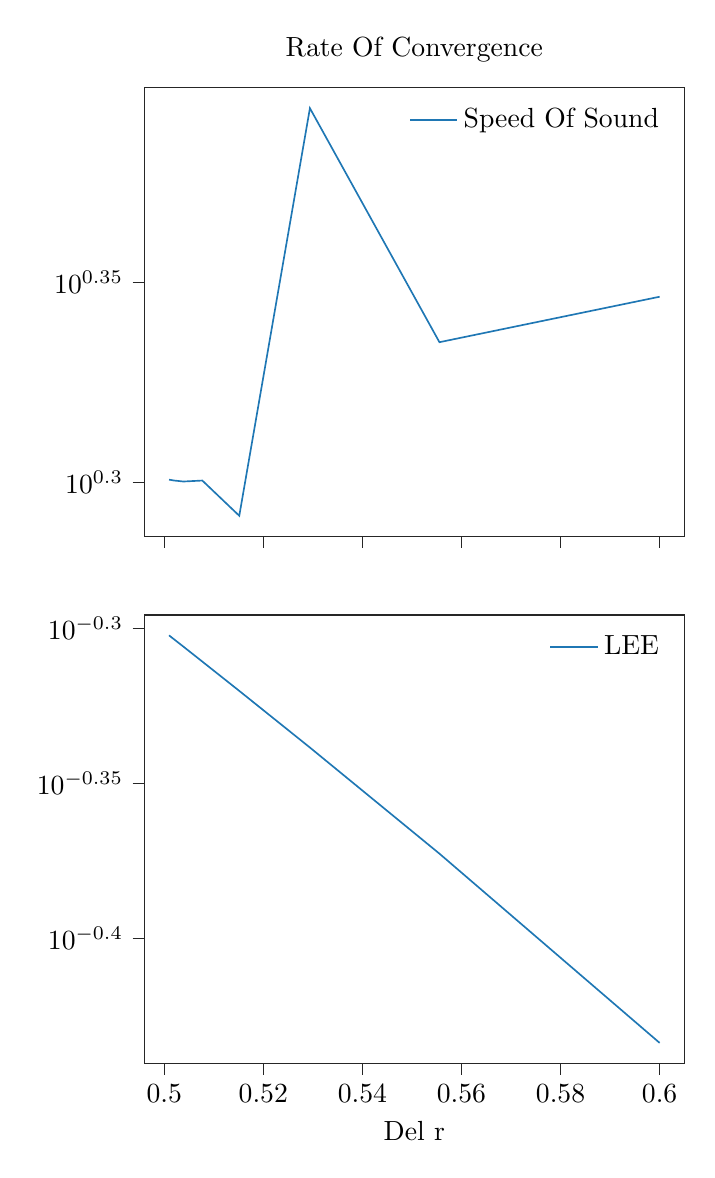
\begin{tikzpicture}

\definecolor{color0}{rgb}{0.12156862745098,0.466666666666667,0.705882352941177}

\begin{groupplot}[group style={group size=1 by 2}]
\nextgroupplot[
axis line style={white!15!black},
legend cell align={left},
legend style={fill opacity=0.8, draw opacity=1, text opacity=1, draw=none},
log basis y={10},
scaled x ticks=manual:{}{\pgfmathparse{#1}},
tick align=outside,
tick pos=left,
title={Rate Of Convergence},
x grid style={white!80!black},
xmin=0.49602339181245, xmax=0.60495126705655,
xtick style={color=white!15!black},
xticklabels={},
y grid style={white!80!black},
ymin=1.93465772282466, ymax=2.50490389113768,
ymode=log,
ytick style={color=white!15!black}
]
\addplot [semithick, color0]
table {%
0.6 2.220755792495
0.555555555556 2.163324274032
0.529411764706 2.475663773488
0.515151515152 1.957508006467
0.507692307692 1.997639457419
0.503875968992 1.996551880759
0.501945525292 1.997726606828
0.500974658869 1.998727064418
};
\addlegendentry{Speed Of Sound}

\nextgroupplot[
axis line style={white!15!black},
legend cell align={left},
legend style={fill opacity=0.8, draw opacity=1, text opacity=1, draw=none},
log basis y={10},
tick align=outside,
tick pos=left,
x grid style={white!80!black},
xlabel={Del r},
xmin=0.49602339181245, xmax=0.60495126705655,
xtick style={color=white!15!black},
y grid style={white!80!black},
ymin=0.362953235346687, ymax=0.506191289267272,
ymode=log,
ytick style={color=white!15!black}
]
\addplot [semithick, color0]
table {%
0.6 0.368482797082
0.555555555556 0.423998453276
0.529411764706 0.458768919907
0.515151515152 0.478465639055
0.507692307692 0.488986846835
0.503875968992 0.494429721197
0.501945525292 0.497198646885
0.500974658869 0.498595233207
};
\addlegendentry{LEE}
\end{groupplot}

\end{tikzpicture}
}
%     \end{center}
%     \caption{Rate of Convergence for the Speed of Sound Integration}
% \end{figure}

% \begin{figure}
%     \begin{center}
%         \scalebox{0.75}{\begin{tikzpicture}[gnuplot]
%% generated with GNUPLOT 5.2p8 (Lua 5.3; terminal rev. Nov 2018, script rev. 108)
%% Fri 17 Sep 2021 01:00:01 PM EDT
\path (0.000,0.000) rectangle (12.500,8.750);
\gpcolor{color=gp lt color axes}
\gpsetlinetype{gp lt axes}
\gpsetdashtype{gp dt axes}
\gpsetlinewidth{0.50}
\draw[gp path] (0.000,7.175)--(11.249,7.175);
\gpcolor{color=gp lt color border}
\gpsetlinetype{gp lt border}
\gpsetdashtype{gp dt solid}
\gpsetlinewidth{1.00}
\draw[gp path] (0.000,7.175)--(0.090,7.175);
\draw[gp path] (11.249,7.175)--(11.159,7.175);
\node[gp node right] at (-0.184,7.175) {$-2.5$};
\gpcolor{color=gp lt color axes}
\gpsetlinetype{gp lt axes}
\gpsetdashtype{gp dt axes}
\gpsetlinewidth{0.50}
\draw[gp path] (0.000,7.455)--(11.249,7.455);
\gpcolor{color=gp lt color border}
\gpsetlinetype{gp lt border}
\gpsetdashtype{gp dt solid}
\gpsetlinewidth{1.00}
\draw[gp path] (0.000,7.455)--(0.090,7.455);
\draw[gp path] (11.249,7.455)--(11.159,7.455);
\node[gp node right] at (-0.184,7.455) {$-2$};
\gpcolor{color=gp lt color axes}
\gpsetlinetype{gp lt axes}
\gpsetdashtype{gp dt axes}
\gpsetlinewidth{0.50}
\draw[gp path] (0.000,7.735)--(11.249,7.735);
\gpcolor{color=gp lt color border}
\gpsetlinetype{gp lt border}
\gpsetdashtype{gp dt solid}
\gpsetlinewidth{1.00}
\draw[gp path] (0.000,7.735)--(0.090,7.735);
\draw[gp path] (11.249,7.735)--(11.159,7.735);
\node[gp node right] at (-0.184,7.735) {$-1.5$};
\gpcolor{color=gp lt color axes}
\gpsetlinetype{gp lt axes}
\gpsetdashtype{gp dt axes}
\gpsetlinewidth{0.50}
\draw[gp path] (0.000,8.014)--(9.413,8.014);
\draw[gp path] (11.065,8.014)--(11.249,8.014);
\gpcolor{color=gp lt color border}
\gpsetlinetype{gp lt border}
\gpsetdashtype{gp dt solid}
\gpsetlinewidth{1.00}
\draw[gp path] (0.000,8.014)--(0.090,8.014);
\draw[gp path] (11.249,8.014)--(11.159,8.014);
\node[gp node right] at (-0.184,8.014) {$-1$};
\gpcolor{color=gp lt color axes}
\gpsetlinetype{gp lt axes}
\gpsetdashtype{gp dt axes}
\gpsetlinewidth{0.50}
\draw[gp path] (0.000,8.294)--(9.413,8.294);
\draw[gp path] (11.065,8.294)--(11.249,8.294);
\gpcolor{color=gp lt color border}
\gpsetlinetype{gp lt border}
\gpsetdashtype{gp dt solid}
\gpsetlinewidth{1.00}
\draw[gp path] (0.000,8.294)--(0.090,8.294);
\draw[gp path] (11.249,8.294)--(11.159,8.294);
\node[gp node right] at (-0.184,8.294) {$-0.5$};
\gpcolor{color=gp lt color axes}
\gpsetlinetype{gp lt axes}
\gpsetdashtype{gp dt axes}
\gpsetlinewidth{0.50}
\draw[gp path] (0.000,8.574)--(11.249,8.574);
\gpcolor{color=gp lt color border}
\gpsetlinetype{gp lt border}
\gpsetdashtype{gp dt solid}
\gpsetlinewidth{1.00}
\draw[gp path] (0.000,8.574)--(0.090,8.574);
\draw[gp path] (11.249,8.574)--(11.159,8.574);
\node[gp node right] at (-0.184,8.574) {$0$};
\gpcolor{color=gp lt color axes}
\gpsetlinetype{gp lt axes}
\gpsetdashtype{gp dt axes}
\gpsetlinewidth{0.50}
\draw[gp path] (0.000,7.175)--(0.000,8.574);
\gpcolor{color=gp lt color border}
\gpsetlinetype{gp lt border}
\gpsetdashtype{gp dt solid}
\gpsetlinewidth{1.00}
\draw[gp path] (0.000,7.175)--(0.000,7.355);
\draw[gp path] (0.000,8.574)--(0.000,8.394);
\node[gp node center] at (0.000,6.867) {$0$};
\gpcolor{color=gp lt color axes}
\gpsetlinetype{gp lt axes}
\gpsetdashtype{gp dt axes}
\gpsetlinewidth{0.50}
\draw[gp path] (1.875,7.175)--(1.875,8.574);
\gpcolor{color=gp lt color border}
\gpsetlinetype{gp lt border}
\gpsetdashtype{gp dt solid}
\gpsetlinewidth{1.00}
\draw[gp path] (1.875,7.175)--(1.875,7.355);
\draw[gp path] (1.875,8.574)--(1.875,8.394);
\node[gp node center] at (1.875,6.867) {$200$};
\gpcolor{color=gp lt color axes}
\gpsetlinetype{gp lt axes}
\gpsetdashtype{gp dt axes}
\gpsetlinewidth{0.50}
\draw[gp path] (3.750,7.175)--(3.750,8.574);
\gpcolor{color=gp lt color border}
\gpsetlinetype{gp lt border}
\gpsetdashtype{gp dt solid}
\gpsetlinewidth{1.00}
\draw[gp path] (3.750,7.175)--(3.750,7.355);
\draw[gp path] (3.750,8.574)--(3.750,8.394);
\node[gp node center] at (3.750,6.867) {$400$};
\gpcolor{color=gp lt color axes}
\gpsetlinetype{gp lt axes}
\gpsetdashtype{gp dt axes}
\gpsetlinewidth{0.50}
\draw[gp path] (5.625,7.175)--(5.625,8.574);
\gpcolor{color=gp lt color border}
\gpsetlinetype{gp lt border}
\gpsetdashtype{gp dt solid}
\gpsetlinewidth{1.00}
\draw[gp path] (5.625,7.175)--(5.625,7.355);
\draw[gp path] (5.625,8.574)--(5.625,8.394);
\node[gp node center] at (5.625,6.867) {$600$};
\gpcolor{color=gp lt color axes}
\gpsetlinetype{gp lt axes}
\gpsetdashtype{gp dt axes}
\gpsetlinewidth{0.50}
\draw[gp path] (7.499,7.175)--(7.499,8.574);
\gpcolor{color=gp lt color border}
\gpsetlinetype{gp lt border}
\gpsetdashtype{gp dt solid}
\gpsetlinewidth{1.00}
\draw[gp path] (7.499,7.175)--(7.499,7.355);
\draw[gp path] (7.499,8.574)--(7.499,8.394);
\node[gp node center] at (7.499,6.867) {$800$};
\gpcolor{color=gp lt color axes}
\gpsetlinetype{gp lt axes}
\gpsetdashtype{gp dt axes}
\gpsetlinewidth{0.50}
\draw[gp path] (9.374,7.175)--(9.374,8.574);
\gpcolor{color=gp lt color border}
\gpsetlinetype{gp lt border}
\gpsetdashtype{gp dt solid}
\gpsetlinewidth{1.00}
\draw[gp path] (9.374,7.175)--(9.374,7.355);
\draw[gp path] (9.374,8.574)--(9.374,8.394);
\node[gp node center] at (9.374,6.867) {$1000$};
\gpcolor{color=gp lt color axes}
\gpsetlinetype{gp lt axes}
\gpsetdashtype{gp dt axes}
\gpsetlinewidth{0.50}
\draw[gp path] (11.249,7.175)--(11.249,8.574);
\gpcolor{color=gp lt color border}
\gpsetlinetype{gp lt border}
\gpsetdashtype{gp dt solid}
\gpsetlinewidth{1.00}
\draw[gp path] (11.249,7.175)--(11.249,7.355);
\draw[gp path] (11.249,8.574)--(11.249,8.394);
\node[gp node center] at (11.249,6.867) {$1200$};
\draw[gp path] (0.000,8.574)--(0.000,7.175)--(11.249,7.175)--(11.249,8.574)--cycle;
\node[gp node right] at (9.781,8.240) {S1};
\gpcolor{rgb color={0.000,0.502,0.502}}
\draw[gp path] (9.965,8.240)--(10.881,8.240);
\draw[gp path] (0.009,7.404)--(0.019,7.407)--(0.028,7.409)--(0.037,7.411)--(0.047,7.413)%
  --(0.056,7.416)--(0.066,7.418)--(0.075,7.420)--(0.084,7.423)--(0.094,7.426)--(0.103,7.428)%
  --(0.112,7.431)--(0.122,7.434)--(0.131,7.436)--(0.141,7.439)--(0.150,7.442)--(0.159,7.445)%
  --(0.169,7.448)--(0.178,7.451)--(0.187,7.454)--(0.197,7.458)--(0.206,7.461)--(0.216,7.464)%
  --(0.225,7.467)--(0.234,7.471)--(0.244,7.474)--(0.253,7.478)--(0.262,7.481)--(0.272,7.485)%
  --(0.281,7.488)--(0.291,7.492)--(0.300,7.495)--(0.309,7.499)--(0.319,7.503)--(0.328,7.507)%
  --(0.337,7.511)--(0.347,7.514)--(0.356,7.518)--(0.366,7.522)--(0.375,7.526)--(0.384,7.530)%
  --(0.394,7.534)--(0.403,7.538)--(0.412,7.542)--(0.422,7.547)--(0.431,7.551)--(0.441,7.555)%
  --(0.450,7.559)--(0.459,7.563)--(0.469,7.568)--(0.478,7.572)--(0.487,7.576)--(0.497,7.581)%
  --(0.506,7.585)--(0.516,7.589)--(0.525,7.594)--(0.534,7.598)--(0.544,7.603)--(0.553,7.607)%
  --(0.562,7.612)--(0.572,7.616)--(0.581,7.621)--(0.591,7.625)--(0.600,7.630)--(0.609,7.634)%
  --(0.619,7.639)--(0.628,7.643)--(0.637,7.648)--(0.647,7.652)--(0.656,7.657)--(0.666,7.662)%
  --(0.675,7.666)--(0.684,7.671)--(0.694,7.675)--(0.703,7.680)--(0.712,7.685)--(0.722,7.689)%
  --(0.731,7.694)--(0.741,7.698)--(0.750,7.703)--(0.759,7.708)--(0.769,7.712)--(0.778,7.717)%
  --(0.787,7.721)--(0.797,7.726)--(0.806,7.731)--(0.816,7.735)--(0.825,7.740)--(0.834,7.744)%
  --(0.844,7.749)--(0.853,7.753)--(0.862,7.758)--(0.872,7.762)--(0.881,7.767)--(0.891,7.771)%
  --(0.900,7.776)--(0.909,7.780)--(0.919,7.785)--(0.928,7.789)--(0.937,7.794)--(0.947,7.798)%
  --(0.956,7.802)--(0.966,7.807)--(0.975,7.811)--(0.984,7.815)--(0.994,7.819)--(1.003,7.824)%
  --(1.012,7.828)--(1.022,7.832)--(1.031,7.836)--(1.041,7.840)--(1.050,7.845)--(1.059,7.849)%
  --(1.069,7.853)--(1.078,7.857)--(1.087,7.861)--(1.097,7.865)--(1.106,7.869)--(1.116,7.873)%
  --(1.125,7.876)--(1.134,7.880)--(1.144,7.884)--(1.153,7.888)--(1.162,7.892)--(1.172,7.895)%
  --(1.181,7.899)--(1.191,7.903)--(1.200,7.906)--(1.209,7.910)--(1.219,7.914)--(1.228,7.917)%
  --(1.237,7.920)--(1.247,7.924)--(1.256,7.927)--(1.266,7.931)--(1.275,7.934)--(1.284,7.937)%
  --(1.294,7.940)--(1.303,7.944)--(1.312,7.947)--(1.322,7.950)--(1.331,7.953)--(1.341,7.956)%
  --(1.350,7.959)--(1.359,7.962)--(1.369,7.965)--(1.378,7.968)--(1.387,7.970)--(1.397,7.973)%
  --(1.406,7.976)--(1.415,7.979)--(1.425,7.981)--(1.434,7.984)--(1.444,7.986)--(1.453,7.989)%
  --(1.462,7.991)--(1.472,7.994)--(1.481,7.996)--(1.490,7.998)--(1.500,8.001)--(1.509,8.003)%
  --(1.519,8.005)--(1.528,8.007)--(1.537,8.009)--(1.547,8.011)--(1.556,8.013)--(1.565,8.015)%
  --(1.575,8.017)--(1.584,8.019)--(1.594,8.020)--(1.603,8.022)--(1.612,8.024)--(1.622,8.025)%
  --(1.631,8.027)--(1.640,8.028)--(1.650,8.030)--(1.659,8.031)--(1.669,8.033)--(1.678,8.034)%
  --(1.687,8.035)--(1.697,8.036)--(1.706,8.037)--(1.715,8.038)--(1.725,8.040)--(1.734,8.041)%
  --(1.744,8.041)--(1.753,8.042)--(1.762,8.043)--(1.772,8.044)--(1.781,8.045)--(1.790,8.045)%
  --(1.800,8.046)--(1.809,8.047)--(1.819,8.047)--(1.828,8.048)--(1.837,8.048)--(1.847,8.048)%
  --(1.856,8.049)--(1.865,8.049)--(1.875,8.049)--(1.884,8.050)--(1.894,8.050)--(1.903,8.050)%
  --(1.912,8.050)--(1.922,8.050)--(1.931,8.050)--(1.940,8.050)--(1.950,8.050)--(1.959,8.049)%
  --(1.969,8.049)--(1.978,8.049)--(1.987,8.049)--(1.997,8.048)--(2.006,8.048)--(2.015,8.047)%
  --(2.025,8.047)--(2.034,8.046)--(2.044,8.046)--(2.053,8.045)--(2.062,8.044)--(2.072,8.044)%
  --(2.081,8.043)--(2.090,8.042)--(2.100,8.041)--(2.109,8.040)--(2.119,8.040)--(2.128,8.039)%
  --(2.137,8.038)--(2.147,8.037)--(2.156,8.036)--(2.165,8.034)--(2.175,8.033)--(2.184,8.032)%
  --(2.194,8.031)--(2.203,8.030)--(2.212,8.028)--(2.222,8.027)--(2.231,8.026)--(2.240,8.024)%
  --(2.250,8.023)--(2.259,8.022)--(2.269,8.020)--(2.278,8.019)--(2.287,8.017)--(2.297,8.016)%
  --(2.306,8.014)--(2.315,8.012)--(2.325,8.011)--(2.334,8.009)--(2.344,8.007)--(2.353,8.006)%
  --(2.362,8.004)--(2.372,8.002)--(2.381,8.000)--(2.390,7.999)--(2.400,7.997)--(2.409,7.995)%
  --(2.419,7.993)--(2.428,7.991)--(2.437,7.989)--(2.447,7.987)--(2.456,7.985)--(2.465,7.984)%
  --(2.475,7.982)--(2.484,7.980)--(2.494,7.978)--(2.503,7.975)--(2.512,7.973)--(2.522,7.971)%
  --(2.531,7.969)--(2.540,7.967)--(2.550,7.965)--(2.559,7.963)--(2.569,7.961)--(2.578,7.959)%
  --(2.587,7.957)--(2.597,7.955)--(2.606,7.952)--(2.615,7.950)--(2.625,7.948)--(2.634,7.946)%
  --(2.644,7.944)--(2.653,7.942)--(2.662,7.939)--(2.672,7.937)--(2.681,7.935)--(2.690,7.933)%
  --(2.700,7.931)--(2.709,7.928)--(2.719,7.926)--(2.728,7.924)--(2.737,7.922)--(2.747,7.920)%
  --(2.756,7.917)--(2.765,7.915)--(2.775,7.913)--(2.784,7.911)--(2.794,7.909)--(2.803,7.907)%
  --(2.812,7.904)--(2.822,7.902)--(2.831,7.900)--(2.840,7.898)--(2.850,7.896)--(2.859,7.894)%
  --(2.868,7.892)--(2.878,7.890)--(2.887,7.888)--(2.897,7.886)--(2.906,7.883)--(2.915,7.881)%
  --(2.925,7.879)--(2.934,7.877)--(2.943,7.875)--(2.953,7.873)--(2.962,7.872)--(2.972,7.870)%
  --(2.981,7.868)--(2.990,7.866)--(3.000,7.864)--(3.009,7.862)--(3.018,7.860)--(3.028,7.859)%
  --(3.037,7.857)--(3.047,7.855)--(3.056,7.853)--(3.065,7.852)--(3.075,7.850)--(3.084,7.848)%
  --(3.093,7.847)--(3.103,7.845)--(3.112,7.844)--(3.122,7.842)--(3.131,7.840)--(3.140,7.839)%
  --(3.150,7.838)--(3.159,7.836)--(3.168,7.835)--(3.178,7.833)--(3.187,7.832)--(3.197,7.831)%
  --(3.206,7.830)--(3.215,7.828)--(3.225,7.827)--(3.234,7.826)--(3.243,7.825)--(3.253,7.824)%
  --(3.262,7.823)--(3.272,7.822)--(3.281,7.821)--(3.290,7.820)--(3.300,7.819)--(3.309,7.818)%
  --(3.318,7.818)--(3.328,7.817)--(3.337,7.816)--(3.347,7.816)--(3.356,7.815)--(3.365,7.814)%
  --(3.375,7.814)--(3.384,7.813)--(3.393,7.813)--(3.403,7.812)--(3.412,7.812)--(3.422,7.812)%
  --(3.431,7.812)--(3.440,7.811)--(3.450,7.811)--(3.459,7.811)--(3.468,7.811)--(3.478,7.811)%
  --(3.487,7.811)--(3.497,7.811)--(3.506,7.811)--(3.515,7.811)--(3.525,7.811)--(3.534,7.811)%
  --(3.543,7.812)--(3.553,7.812)--(3.562,7.812)--(3.572,7.813)--(3.581,7.813)--(3.590,7.814)%
  --(3.600,7.814)--(3.609,7.815)--(3.618,7.816)--(3.628,7.816)--(3.637,7.817)--(3.647,7.818)%
  --(3.656,7.819)--(3.665,7.820)--(3.675,7.820)--(3.684,7.821)--(3.693,7.822)--(3.703,7.823)%
  --(3.712,7.825)--(3.722,7.826)--(3.731,7.827)--(3.740,7.828)--(3.750,7.829)--(3.759,7.831)%
  --(3.768,7.832)--(3.778,7.833)--(3.787,7.835)--(3.797,7.836)--(3.806,7.838)--(3.815,7.840)%
  --(3.825,7.841)--(3.834,7.843)--(3.843,7.844)--(3.853,7.846)--(3.862,7.848)--(3.872,7.850)%
  --(3.881,7.852)--(3.890,7.854)--(3.900,7.855)--(3.909,7.857)--(3.918,7.859)--(3.928,7.861)%
  --(3.937,7.864)--(3.947,7.866)--(3.956,7.868)--(3.965,7.870)--(3.975,7.872)--(3.984,7.874)%
  --(3.993,7.877)--(4.003,7.879)--(4.012,7.881)--(4.022,7.884)--(4.031,7.886)--(4.040,7.888)%
  --(4.050,7.891)--(4.059,7.893)--(4.068,7.896)--(4.078,7.898)--(4.087,7.901)--(4.097,7.904)%
  --(4.106,7.906)--(4.115,7.909)--(4.125,7.911)--(4.134,7.914)--(4.143,7.917)--(4.153,7.920)%
  --(4.162,7.922)--(4.172,7.925)--(4.181,7.928)--(4.190,7.931)--(4.200,7.934)--(4.209,7.936)%
  --(4.218,7.939)--(4.228,7.942)--(4.237,7.945)--(4.246,7.948)--(4.256,7.951)--(4.265,7.954)%
  --(4.275,7.957)--(4.284,7.960)--(4.293,7.963)--(4.303,7.966)--(4.312,7.969)--(4.321,7.972)%
  --(4.331,7.975)--(4.340,7.978)--(4.350,7.981)--(4.359,7.984)--(4.368,7.987)--(4.378,7.990)%
  --(4.387,7.993)--(4.396,7.996)--(4.406,8.000)--(4.415,8.003)--(4.425,8.006)--(4.434,8.009)%
  --(4.443,8.012)--(4.453,8.015)--(4.462,8.018)--(4.471,8.021)--(4.481,8.025)--(4.490,8.028)%
  --(4.500,8.031)--(4.509,8.034)--(4.518,8.037)--(4.528,8.040)--(4.537,8.043)--(4.546,8.047)%
  --(4.556,8.050)--(4.565,8.053)--(4.575,8.056)--(4.584,8.059)--(4.593,8.062)--(4.603,8.065)%
  --(4.612,8.069)--(4.621,8.072)--(4.631,8.075)--(4.640,8.078)--(4.650,8.081)--(4.659,8.084)%
  --(4.668,8.087)--(4.678,8.090)--(4.687,8.093)--(4.696,8.097)--(4.706,8.100)--(4.715,8.103)%
  --(4.725,8.106)--(4.734,8.109)--(4.743,8.112)--(4.753,8.115)--(4.762,8.118)--(4.771,8.121)%
  --(4.781,8.124)--(4.790,8.127)--(4.800,8.130)--(4.809,8.133)--(4.818,8.136)--(4.828,8.139)%
  --(4.837,8.142)--(4.846,8.145)--(4.856,8.148)--(4.865,8.151)--(4.875,8.154)--(4.884,8.156)%
  --(4.893,8.159)--(4.903,8.162)--(4.912,8.165)--(4.921,8.168)--(4.931,8.171)--(4.940,8.174)%
  --(4.950,8.176)--(4.959,8.179)--(4.968,8.182)--(4.978,8.185)--(4.987,8.188)--(4.996,8.190)%
  --(5.006,8.193)--(5.015,8.196)--(5.025,8.199)--(5.034,8.201)--(5.043,8.204)--(5.053,8.207)%
  --(5.062,8.209)--(5.071,8.212)--(5.081,8.214)--(5.090,8.217)--(5.100,8.220)--(5.109,8.222)%
  --(5.118,8.225)--(5.128,8.227)--(5.137,8.230)--(5.146,8.232)--(5.156,8.235)--(5.165,8.237)%
  --(5.175,8.240)--(5.184,8.242)--(5.193,8.245)--(5.203,8.247)--(5.212,8.250)--(5.221,8.252)%
  --(5.231,8.254)--(5.240,8.257)--(5.250,8.259)--(5.259,8.262)--(5.268,8.264)--(5.278,8.266)%
  --(5.287,8.268)--(5.296,8.271)--(5.306,8.273)--(5.315,8.275)--(5.325,8.278)--(5.334,8.280)%
  --(5.343,8.282)--(5.353,8.284)--(5.362,8.286)--(5.371,8.288)--(5.381,8.291)--(5.390,8.293)%
  --(5.400,8.295)--(5.409,8.297)--(5.418,8.299)--(5.428,8.301)--(5.437,8.303)--(5.446,8.305)%
  --(5.456,8.307)--(5.465,8.309)--(5.475,8.311)--(5.484,8.313)--(5.493,8.315)--(5.503,8.317)%
  --(5.512,8.319)--(5.521,8.321)--(5.531,8.323)--(5.540,8.325)--(5.550,8.326)--(5.559,8.328)%
  --(5.568,8.330)--(5.578,8.332)--(5.587,8.334)--(5.596,8.335)--(5.606,8.337)--(5.615,8.339)%
  --(5.625,8.341)--(5.634,8.342)--(5.643,8.344)--(5.653,8.346)--(5.662,8.348)--(5.671,8.349)%
  --(5.681,8.351)--(5.690,8.352)--(5.699,8.354)--(5.709,8.356)--(5.718,8.357)--(5.728,8.359)%
  --(5.737,8.360)--(5.746,8.362)--(5.756,8.363)--(5.765,8.365)--(5.774,8.366)--(5.784,8.368)%
  --(5.793,8.369)--(5.803,8.371)--(5.812,8.372)--(5.821,8.374)--(5.831,8.375)--(5.840,8.376)%
  --(5.849,8.378)--(5.859,8.379)--(5.868,8.380)--(5.878,8.382)--(5.887,8.383)--(5.896,8.384)%
  --(5.906,8.386)--(5.915,8.387)--(5.924,8.388)--(5.934,8.389)--(5.943,8.391)--(5.953,8.392)%
  --(5.962,8.393)--(5.971,8.394)--(5.981,8.395)--(5.990,8.396)--(5.999,8.398)--(6.009,8.399)%
  --(6.018,8.400)--(6.028,8.401)--(6.037,8.402)--(6.046,8.403)--(6.056,8.404)--(6.065,8.405)%
  --(6.074,8.406)--(6.084,8.407)--(6.093,8.408)--(6.103,8.409)--(6.112,8.410)--(6.121,8.411)%
  --(6.131,8.412)--(6.140,8.413)--(6.149,8.413)--(6.159,8.414)--(6.168,8.415)--(6.178,8.416)%
  --(6.187,8.417)--(6.196,8.418)--(6.206,8.418)--(6.215,8.419)--(6.224,8.420)--(6.234,8.421)%
  --(6.243,8.421)--(6.253,8.422)--(6.262,8.423)--(6.271,8.423)--(6.281,8.424)--(6.290,8.425)%
  --(6.299,8.425)--(6.309,8.426)--(6.318,8.427)--(6.328,8.427)--(6.337,8.428)--(6.346,8.428)%
  --(6.356,8.429)--(6.365,8.429)--(6.374,8.430)--(6.384,8.430)--(6.393,8.431)--(6.403,8.431)%
  --(6.412,8.432)--(6.421,8.432)--(6.431,8.432)--(6.440,8.433)--(6.449,8.433)--(6.459,8.433)%
  --(6.468,8.434)--(6.478,8.434)--(6.487,8.434)--(6.496,8.435)--(6.506,8.435)--(6.515,8.435)%
  --(6.524,8.435)--(6.534,8.436)--(6.543,8.436)--(6.553,8.436)--(6.562,8.436)--(6.571,8.436)%
  --(6.581,8.436)--(6.590,8.437)--(6.599,8.437)--(6.609,8.437)--(6.618,8.437)--(6.628,8.437)%
  --(6.637,8.437)--(6.646,8.437)--(6.656,8.437)--(6.665,8.437)--(6.674,8.437)--(6.684,8.437)%
  --(6.693,8.437)--(6.703,8.437)--(6.712,8.437)--(6.721,8.436)--(6.731,8.436)--(6.740,8.436)%
  --(6.749,8.436)--(6.759,8.436)--(6.768,8.436)--(6.778,8.435)--(6.787,8.435)--(6.796,8.435)%
  --(6.806,8.435)--(6.815,8.434)--(6.824,8.434)--(6.834,8.434)--(6.843,8.434)--(6.853,8.433)%
  --(6.862,8.433)--(6.871,8.433)--(6.881,8.432)--(6.890,8.432)--(6.899,8.431)--(6.909,8.431)%
  --(6.918,8.431)--(6.928,8.430)--(6.937,8.430)--(6.946,8.429)--(6.956,8.429)--(6.965,8.428)%
  --(6.974,8.428)--(6.984,8.427)--(6.993,8.427)--(7.003,8.426)--(7.012,8.425)--(7.021,8.425)%
  --(7.031,8.424)--(7.040,8.424)--(7.049,8.423)--(7.059,8.422)--(7.068,8.422)--(7.077,8.421)%
  --(7.087,8.420)--(7.096,8.420)--(7.106,8.419)--(7.115,8.418)--(7.124,8.417)--(7.134,8.417)%
  --(7.143,8.416)--(7.152,8.415)--(7.162,8.414)--(7.171,8.414)--(7.181,8.413)--(7.190,8.412)%
  --(7.199,8.411)--(7.209,8.410)--(7.218,8.409)--(7.227,8.409)--(7.237,8.408)--(7.246,8.407)%
  --(7.256,8.406)--(7.265,8.405)--(7.274,8.404)--(7.284,8.403)--(7.293,8.402)--(7.302,8.401)%
  --(7.312,8.400)--(7.321,8.399)--(7.331,8.398)--(7.340,8.397)--(7.349,8.396)--(7.359,8.395)%
  --(7.368,8.394)--(7.377,8.393)--(7.387,8.392)--(7.396,8.391)--(7.406,8.390)--(7.415,8.388)%
  --(7.424,8.387)--(7.434,8.386)--(7.443,8.385)--(7.452,8.384)--(7.462,8.383)--(7.471,8.381)%
  --(7.481,8.380)--(7.490,8.379)--(7.499,8.378)--(7.509,8.377)--(7.518,8.375)--(7.527,8.374)%
  --(7.537,8.373)--(7.546,8.372)--(7.556,8.370)--(7.565,8.369)--(7.574,8.368)--(7.584,8.366)%
  --(7.593,8.365)--(7.602,8.364)--(7.612,8.362)--(7.621,8.361)--(7.631,8.360)--(7.640,8.358)%
  --(7.649,8.357)--(7.659,8.355)--(7.668,8.354)--(7.677,8.353)--(7.687,8.351)--(7.696,8.350)%
  --(7.706,8.348)--(7.715,8.347)--(7.724,8.345)--(7.734,8.344)--(7.743,8.342)--(7.752,8.341)%
  --(7.762,8.339)--(7.771,8.338)--(7.781,8.336)--(7.790,8.335)--(7.799,8.333)--(7.809,8.331)%
  --(7.818,8.330)--(7.827,8.328)--(7.837,8.327)--(7.846,8.325)--(7.856,8.323)--(7.865,8.322)%
  --(7.874,8.320)--(7.884,8.318)--(7.893,8.317)--(7.902,8.315)--(7.912,8.313)--(7.921,8.312)%
  --(7.931,8.310)--(7.940,8.308)--(7.949,8.307)--(7.959,8.305)--(7.968,8.303)--(7.977,8.301)%
  --(7.987,8.300)--(7.996,8.298)--(8.006,8.296)--(8.015,8.294)--(8.024,8.292)--(8.034,8.291)%
  --(8.043,8.289)--(8.052,8.287)--(8.062,8.285)--(8.071,8.283)--(8.081,8.281)--(8.090,8.280)%
  --(8.099,8.278)--(8.109,8.276)--(8.118,8.274)--(8.127,8.272)--(8.137,8.270)--(8.146,8.268)%
  --(8.156,8.266)--(8.165,8.264)--(8.174,8.262)--(8.184,8.260)--(8.193,8.258)--(8.202,8.256)%
  --(8.212,8.254)--(8.221,8.252)--(8.231,8.251)--(8.240,8.249)--(8.249,8.247)--(8.259,8.245)%
  --(8.268,8.242)--(8.277,8.240)--(8.287,8.238)--(8.296,8.236)--(8.306,8.234)--(8.315,8.232)%
  --(8.324,8.230)--(8.334,8.228)--(8.343,8.226)--(8.352,8.224)--(8.362,8.222)--(8.371,8.220)%
  --(8.381,8.218)--(8.390,8.216)--(8.399,8.214)--(8.409,8.212)--(8.418,8.210)--(8.427,8.207)%
  --(8.437,8.205)--(8.446,8.203)--(8.455,8.201)--(8.465,8.199)--(8.474,8.197)--(8.484,8.195)%
  --(8.493,8.193)--(8.502,8.191)--(8.512,8.188)--(8.521,8.186)--(8.530,8.184)--(8.540,8.182)%
  --(8.549,8.180)--(8.559,8.178)--(8.568,8.176)--(8.577,8.174)--(8.587,8.171)--(8.596,8.169)%
  --(8.605,8.167)--(8.615,8.165)--(8.624,8.163)--(8.634,8.161)--(8.643,8.159)--(8.652,8.157)%
  --(8.662,8.155)--(8.671,8.152)--(8.680,8.150)--(8.690,8.148)--(8.699,8.146)--(8.709,8.144)%
  --(8.718,8.142)--(8.727,8.140)--(8.737,8.138)--(8.746,8.136)--(8.755,8.134)--(8.765,8.132)%
  --(8.774,8.130)--(8.784,8.128)--(8.793,8.126)--(8.802,8.124)--(8.812,8.122)--(8.821,8.120)%
  --(8.830,8.118)--(8.840,8.116)--(8.849,8.114)--(8.859,8.112)--(8.868,8.110)--(8.877,8.108)%
  --(8.887,8.106)--(8.896,8.104)--(8.905,8.102)--(8.915,8.100)--(8.924,8.098)--(8.934,8.097)%
  --(8.943,8.095)--(8.952,8.093)--(8.962,8.091)--(8.971,8.089)--(8.980,8.088)--(8.990,8.086)%
  --(8.999,8.084)--(9.009,8.082)--(9.018,8.081)--(9.027,8.079)--(9.037,8.077)--(9.046,8.076)%
  --(9.055,8.074)--(9.065,8.073)--(9.074,8.071)--(9.084,8.070)--(9.093,8.068)--(9.102,8.066)%
  --(9.112,8.065)--(9.121,8.064)--(9.130,8.062)--(9.140,8.061)--(9.149,8.059)--(9.159,8.058)%
  --(9.168,8.057)--(9.177,8.055)--(9.187,8.054)--(9.196,8.053)--(9.205,8.052)--(9.215,8.050)%
  --(9.224,8.049)--(9.234,8.048)--(9.243,8.047)--(9.252,8.046)--(9.262,8.045)--(9.271,8.044)%
  --(9.280,8.043)--(9.290,8.042)--(9.299,8.041)--(9.309,8.040)--(9.318,8.039)--(9.327,8.038)%
  --(9.337,8.037)--(9.346,8.037)--(9.355,8.036)--(9.365,8.035)--(9.374,8.034)--(9.384,8.034)%
  --(9.393,8.033)--(9.402,8.033)--(9.412,8.032)--(9.421,8.032)--(9.430,8.031)--(9.440,8.031)%
  --(9.449,8.030)--(9.459,8.030)--(9.468,8.030)--(9.477,8.029)--(9.487,8.029)--(9.496,8.029)%
  --(9.505,8.029)--(9.515,8.028)--(9.524,8.028)--(9.534,8.028)--(9.543,8.028)--(9.552,8.028)%
  --(9.562,8.028)--(9.571,8.028)--(9.580,8.028)--(9.590,8.028)--(9.599,8.028)--(9.609,8.029);
\gpsetpointsize{4.00}
\gppoint{gp mark 1}{(0.009,7.404)}
\gppoint{gp mark 1}{(0.103,7.428)}
\gppoint{gp mark 1}{(0.197,7.458)}
\gppoint{gp mark 1}{(0.291,7.492)}
\gppoint{gp mark 1}{(0.384,7.530)}
\gppoint{gp mark 1}{(0.478,7.572)}
\gppoint{gp mark 1}{(0.572,7.616)}
\gppoint{gp mark 1}{(0.666,7.662)}
\gppoint{gp mark 1}{(0.759,7.708)}
\gppoint{gp mark 1}{(0.853,7.753)}
\gppoint{gp mark 1}{(0.947,7.798)}
\gppoint{gp mark 1}{(1.041,7.840)}
\gppoint{gp mark 1}{(1.134,7.880)}
\gppoint{gp mark 1}{(1.228,7.917)}
\gppoint{gp mark 1}{(1.322,7.950)}
\gppoint{gp mark 1}{(1.415,7.979)}
\gppoint{gp mark 1}{(1.509,8.003)}
\gppoint{gp mark 1}{(1.603,8.022)}
\gppoint{gp mark 1}{(1.697,8.036)}
\gppoint{gp mark 1}{(1.790,8.045)}
\gppoint{gp mark 1}{(1.884,8.050)}
\gppoint{gp mark 1}{(1.978,8.049)}
\gppoint{gp mark 1}{(2.072,8.044)}
\gppoint{gp mark 1}{(2.165,8.034)}
\gppoint{gp mark 1}{(2.259,8.022)}
\gppoint{gp mark 1}{(2.353,8.006)}
\gppoint{gp mark 1}{(2.447,7.987)}
\gppoint{gp mark 1}{(2.540,7.967)}
\gppoint{gp mark 1}{(2.634,7.946)}
\gppoint{gp mark 1}{(2.728,7.924)}
\gppoint{gp mark 1}{(2.822,7.902)}
\gppoint{gp mark 1}{(2.915,7.881)}
\gppoint{gp mark 1}{(3.009,7.862)}
\gppoint{gp mark 1}{(3.103,7.845)}
\gppoint{gp mark 1}{(3.197,7.831)}
\gppoint{gp mark 1}{(3.290,7.820)}
\gppoint{gp mark 1}{(3.384,7.813)}
\gppoint{gp mark 1}{(3.478,7.811)}
\gppoint{gp mark 1}{(3.572,7.813)}
\gppoint{gp mark 1}{(3.665,7.820)}
\gppoint{gp mark 1}{(3.759,7.831)}
\gppoint{gp mark 1}{(3.853,7.846)}
\gppoint{gp mark 1}{(3.947,7.866)}
\gppoint{gp mark 1}{(4.040,7.888)}
\gppoint{gp mark 1}{(4.134,7.914)}
\gppoint{gp mark 1}{(4.228,7.942)}
\gppoint{gp mark 1}{(4.321,7.972)}
\gppoint{gp mark 1}{(4.415,8.003)}
\gppoint{gp mark 1}{(4.509,8.034)}
\gppoint{gp mark 1}{(4.603,8.065)}
\gppoint{gp mark 1}{(4.696,8.097)}
\gppoint{gp mark 1}{(4.790,8.127)}
\gppoint{gp mark 1}{(4.884,8.156)}
\gppoint{gp mark 1}{(4.978,8.185)}
\gppoint{gp mark 1}{(5.071,8.212)}
\gppoint{gp mark 1}{(5.165,8.237)}
\gppoint{gp mark 1}{(5.259,8.262)}
\gppoint{gp mark 1}{(5.353,8.284)}
\gppoint{gp mark 1}{(5.446,8.305)}
\gppoint{gp mark 1}{(5.540,8.325)}
\gppoint{gp mark 1}{(5.634,8.342)}
\gppoint{gp mark 1}{(5.728,8.359)}
\gppoint{gp mark 1}{(5.821,8.374)}
\gppoint{gp mark 1}{(5.915,8.387)}
\gppoint{gp mark 1}{(6.009,8.399)}
\gppoint{gp mark 1}{(6.103,8.409)}
\gppoint{gp mark 1}{(6.196,8.418)}
\gppoint{gp mark 1}{(6.290,8.425)}
\gppoint{gp mark 1}{(6.384,8.430)}
\gppoint{gp mark 1}{(6.478,8.434)}
\gppoint{gp mark 1}{(6.571,8.436)}
\gppoint{gp mark 1}{(6.665,8.437)}
\gppoint{gp mark 1}{(6.759,8.436)}
\gppoint{gp mark 1}{(6.853,8.433)}
\gppoint{gp mark 1}{(6.946,8.429)}
\gppoint{gp mark 1}{(7.040,8.424)}
\gppoint{gp mark 1}{(7.134,8.417)}
\gppoint{gp mark 1}{(7.227,8.409)}
\gppoint{gp mark 1}{(7.321,8.399)}
\gppoint{gp mark 1}{(7.415,8.388)}
\gppoint{gp mark 1}{(7.509,8.377)}
\gppoint{gp mark 1}{(7.602,8.364)}
\gppoint{gp mark 1}{(7.696,8.350)}
\gppoint{gp mark 1}{(7.790,8.335)}
\gppoint{gp mark 1}{(7.884,8.318)}
\gppoint{gp mark 1}{(7.977,8.301)}
\gppoint{gp mark 1}{(8.071,8.283)}
\gppoint{gp mark 1}{(8.165,8.264)}
\gppoint{gp mark 1}{(8.259,8.245)}
\gppoint{gp mark 1}{(8.352,8.224)}
\gppoint{gp mark 1}{(8.446,8.203)}
\gppoint{gp mark 1}{(8.540,8.182)}
\gppoint{gp mark 1}{(8.634,8.161)}
\gppoint{gp mark 1}{(8.727,8.140)}
\gppoint{gp mark 1}{(8.821,8.120)}
\gppoint{gp mark 1}{(8.915,8.100)}
\gppoint{gp mark 1}{(9.009,8.082)}
\gppoint{gp mark 1}{(9.102,8.066)}
\gppoint{gp mark 1}{(9.196,8.053)}
\gppoint{gp mark 1}{(9.290,8.042)}
\gppoint{gp mark 1}{(9.384,8.034)}
\gppoint{gp mark 1}{(9.477,8.029)}
\gppoint{gp mark 1}{(9.571,8.028)}
\gppoint{gp mark 1}{(10.423,8.240)}
\gpcolor{color=gp lt color border}
\node[gp node right] at (9.781,7.932) {S1};
\gpcolor{rgb color={0.000,0.063,0.502}}
\draw[gp path] (9.965,7.932)--(10.881,7.932);
\draw[gp path] (0.009,8.574)--(0.019,7.488)--(0.028,7.491)--(0.037,7.493)--(0.047,7.495)%
  --(0.056,7.498)--(0.066,7.500)--(0.075,7.502)--(0.084,7.505)--(0.094,7.507)--(0.103,7.510)%
  --(0.112,7.513)--(0.122,7.515)--(0.131,7.518)--(0.141,7.521)--(0.150,7.524)--(0.159,7.527)%
  --(0.169,7.530)--(0.178,7.532)--(0.187,7.535)--(0.197,7.538)--(0.206,7.542)--(0.216,7.545)%
  --(0.225,7.548)--(0.234,7.551)--(0.244,7.554)--(0.253,7.557)--(0.262,7.561)--(0.272,7.564)%
  --(0.281,7.567)--(0.291,7.571)--(0.300,7.574)--(0.309,7.578)--(0.319,7.581)--(0.328,7.585)%
  --(0.337,7.588)--(0.347,7.592)--(0.356,7.596)--(0.366,7.599)--(0.375,7.603)--(0.384,7.607)%
  --(0.394,7.610)--(0.403,7.614)--(0.412,7.618)--(0.422,7.622)--(0.431,7.626)--(0.441,7.629)%
  --(0.450,7.633)--(0.459,7.637)--(0.469,7.641)--(0.478,7.645)--(0.487,7.649)--(0.497,7.653)%
  --(0.506,7.657)--(0.516,7.661)--(0.525,7.665)--(0.534,7.669)--(0.544,7.673)--(0.553,7.677)%
  --(0.562,7.681)--(0.572,7.685)--(0.581,7.689)--(0.591,7.694)--(0.600,7.698)--(0.609,7.702)%
  --(0.619,7.706)--(0.628,7.710)--(0.637,7.714)--(0.647,7.718)--(0.656,7.723)--(0.666,7.727)%
  --(0.675,7.731)--(0.684,7.735)--(0.694,7.739)--(0.703,7.744)--(0.712,7.748)--(0.722,7.752)%
  --(0.731,7.756)--(0.741,7.760)--(0.750,7.764)--(0.759,7.769)--(0.769,7.773)--(0.778,7.777)%
  --(0.787,7.781)--(0.797,7.785)--(0.806,7.789)--(0.816,7.793)--(0.825,7.798)--(0.834,7.802)%
  --(0.844,7.806)--(0.853,7.810)--(0.862,7.814)--(0.872,7.818)--(0.881,7.822)--(0.891,7.826)%
  --(0.900,7.830)--(0.909,7.834)--(0.919,7.838)--(0.928,7.842)--(0.937,7.846)--(0.947,7.850)%
  --(0.956,7.854)--(0.966,7.858)--(0.975,7.862)--(0.984,7.866)--(0.994,7.870)--(1.003,7.874)%
  --(1.012,7.877)--(1.022,7.881)--(1.031,7.885)--(1.041,7.889)--(1.050,7.893)--(1.059,7.896)%
  --(1.069,7.900)--(1.078,7.904)--(1.087,7.907)--(1.097,7.911)--(1.106,7.914)--(1.116,7.918)%
  --(1.125,7.922)--(1.134,7.925)--(1.144,7.929)--(1.153,7.932)--(1.162,7.935)--(1.172,7.939)%
  --(1.181,7.942)--(1.191,7.945)--(1.200,7.949)--(1.209,7.952)--(1.219,7.955)--(1.228,7.958)%
  --(1.237,7.962)--(1.247,7.965)--(1.256,7.968)--(1.266,7.971)--(1.275,7.974)--(1.284,7.977)%
  --(1.294,7.980)--(1.303,7.983)--(1.312,7.986)--(1.322,7.989)--(1.331,7.991)--(1.341,7.994)%
  --(1.350,7.997)--(1.359,8.000)--(1.369,8.002)--(1.378,8.005)--(1.387,8.007)--(1.397,8.010)%
  --(1.406,8.012)--(1.415,8.015)--(1.425,8.017)--(1.434,8.020)--(1.444,8.022)--(1.453,8.024)%
  --(1.462,8.027)--(1.472,8.029)--(1.481,8.031)--(1.490,8.033)--(1.500,8.035)--(1.509,8.037)%
  --(1.519,8.039)--(1.528,8.041)--(1.537,8.043)--(1.547,8.045)--(1.556,8.047)--(1.565,8.048)%
  --(1.575,8.050)--(1.584,8.052)--(1.594,8.054)--(1.603,8.055)--(1.612,8.057)--(1.622,8.058)%
  --(1.631,8.060)--(1.640,8.061)--(1.650,8.062)--(1.659,8.064)--(1.669,8.065)--(1.678,8.066)%
  --(1.687,8.067)--(1.697,8.069)--(1.706,8.070)--(1.715,8.071)--(1.725,8.072)--(1.734,8.073)%
  --(1.744,8.074)--(1.753,8.074)--(1.762,8.075)--(1.772,8.076)--(1.781,8.077)--(1.790,8.077)%
  --(1.800,8.078)--(1.809,8.079)--(1.819,8.079)--(1.828,8.080)--(1.837,8.080)--(1.847,8.081)%
  --(1.856,8.081)--(1.865,8.081)--(1.875,8.082)--(1.884,8.082)--(1.894,8.082)--(1.903,8.082)%
  --(1.912,8.082)--(1.922,8.082)--(1.931,8.082)--(1.940,8.082)--(1.950,8.082)--(1.959,8.082)%
  --(1.969,8.082)--(1.978,8.082)--(1.987,8.082)--(1.997,8.082)--(2.006,8.081)--(2.015,8.081)%
  --(2.025,8.081)--(2.034,8.080)--(2.044,8.080)--(2.053,8.079)--(2.062,8.079)--(2.072,8.078)%
  --(2.081,8.078)--(2.090,8.077)--(2.100,8.076)--(2.109,8.076)--(2.119,8.075)--(2.128,8.074)%
  --(2.137,8.073)--(2.147,8.073)--(2.156,8.072)--(2.165,8.071)--(2.175,8.070)--(2.184,8.069)%
  --(2.194,8.068)--(2.203,8.067)--(2.212,8.066)--(2.222,8.065)--(2.231,8.064)--(2.240,8.063)%
  --(2.250,8.062)--(2.259,8.060)--(2.269,8.059)--(2.278,8.058)--(2.287,8.057)--(2.297,8.056)%
  --(2.306,8.054)--(2.315,8.053)--(2.325,8.052)--(2.334,8.050)--(2.344,8.049)--(2.353,8.047)%
  --(2.362,8.046)--(2.372,8.045)--(2.381,8.043)--(2.390,8.042)--(2.400,8.040)--(2.409,8.039)%
  --(2.419,8.037)--(2.428,8.036)--(2.437,8.034)--(2.447,8.033)--(2.456,8.031)--(2.465,8.029)%
  --(2.475,8.028)--(2.484,8.026)--(2.494,8.025)--(2.503,8.023)--(2.512,8.021)--(2.522,8.020)%
  --(2.531,8.018)--(2.540,8.016)--(2.550,8.015)--(2.559,8.013)--(2.569,8.011)--(2.578,8.010)%
  --(2.587,8.008)--(2.597,8.006)--(2.606,8.004)--(2.615,8.003)--(2.625,8.001)--(2.634,7.999)%
  --(2.644,7.998)--(2.653,7.996)--(2.662,7.994)--(2.672,7.992)--(2.681,7.991)--(2.690,7.989)%
  --(2.700,7.987)--(2.709,7.985)--(2.719,7.984)--(2.728,7.982)--(2.737,7.980)--(2.747,7.979)%
  --(2.756,7.977)--(2.765,7.975)--(2.775,7.973)--(2.784,7.972)--(2.794,7.970)--(2.803,7.968)%
  --(2.812,7.967)--(2.822,7.965)--(2.831,7.963)--(2.840,7.962)--(2.850,7.960)--(2.859,7.959)%
  --(2.868,7.957)--(2.878,7.955)--(2.887,7.954)--(2.897,7.952)--(2.906,7.951)--(2.915,7.949)%
  --(2.925,7.948)--(2.934,7.946)--(2.943,7.945)--(2.953,7.943)--(2.962,7.942)--(2.972,7.940)%
  --(2.981,7.939)--(2.990,7.937)--(3.000,7.936)--(3.009,7.935)--(3.018,7.933)--(3.028,7.932)%
  --(3.037,7.931)--(3.047,7.929)--(3.056,7.928)--(3.065,7.927)--(3.075,7.926)--(3.084,7.924)%
  --(3.093,7.923)--(3.103,7.922)--(3.112,7.921)--(3.122,7.920)--(3.131,7.919)--(3.140,7.918)%
  --(3.150,7.917)--(3.159,7.916)--(3.168,7.915)--(3.178,7.914)--(3.187,7.913)--(3.197,7.912)%
  --(3.206,7.911)--(3.215,7.910)--(3.225,7.910)--(3.234,7.909)--(3.243,7.908)--(3.253,7.907)%
  --(3.262,7.907)--(3.272,7.906)--(3.281,7.905)--(3.290,7.905)--(3.300,7.904)--(3.309,7.904)%
  --(3.318,7.903)--(3.328,7.903)--(3.337,7.902)--(3.347,7.902)--(3.356,7.902)--(3.365,7.901)%
  --(3.375,7.901)--(3.384,7.901)--(3.393,7.901)--(3.403,7.900)--(3.412,7.900)--(3.422,7.900)%
  --(3.431,7.900)--(3.440,7.900)--(3.450,7.900)--(3.459,7.900)--(3.468,7.900)--(3.478,7.900)%
  --(3.487,7.900)--(3.497,7.901)--(3.506,7.901)--(3.515,7.901)--(3.525,7.901)--(3.534,7.902)%
  --(3.543,7.902)--(3.553,7.902)--(3.562,7.903)--(3.572,7.903)--(3.581,7.904)--(3.590,7.904)%
  --(3.600,7.905)--(3.609,7.905)--(3.618,7.906)--(3.628,7.907)--(3.637,7.907)--(3.647,7.908)%
  --(3.656,7.909)--(3.665,7.910)--(3.675,7.910)--(3.684,7.911)--(3.693,7.912)--(3.703,7.913)%
  --(3.712,7.914)--(3.722,7.915)--(3.731,7.916)--(3.740,7.917)--(3.750,7.918)--(3.759,7.920)%
  --(3.768,7.921)--(3.778,7.922)--(3.787,7.923)--(3.797,7.925)--(3.806,7.926)--(3.815,7.927)%
  --(3.825,7.929)--(3.834,7.930)--(3.843,7.931)--(3.853,7.933)--(3.862,7.934)--(3.872,7.936)%
  --(3.881,7.937)--(3.890,7.939)--(3.900,7.941)--(3.909,7.942)--(3.918,7.944)--(3.928,7.946)%
  --(3.937,7.947)--(3.947,7.949)--(3.956,7.951)--(3.965,7.953)--(3.975,7.955)--(3.984,7.956)%
  --(3.993,7.958)--(4.003,7.960)--(4.012,7.962)--(4.022,7.964)--(4.031,7.966)--(4.040,7.968)%
  --(4.050,7.970)--(4.059,7.972)--(4.068,7.974)--(4.078,7.976)--(4.087,7.978)--(4.097,7.981)%
  --(4.106,7.983)--(4.115,7.985)--(4.125,7.987)--(4.134,7.989)--(4.143,7.992)--(4.153,7.994)%
  --(4.162,7.996)--(4.172,7.998)--(4.181,8.001)--(4.190,8.003)--(4.200,8.005)--(4.209,8.008)%
  --(4.218,8.010)--(4.228,8.012)--(4.237,8.015)--(4.246,8.017)--(4.256,8.020)--(4.265,8.022)%
  --(4.275,8.025)--(4.284,8.027)--(4.293,8.029)--(4.303,8.032)--(4.312,8.034)--(4.321,8.037)%
  --(4.331,8.039)--(4.340,8.042)--(4.350,8.044)--(4.359,8.047)--(4.368,8.050)--(4.378,8.052)%
  --(4.387,8.055)--(4.396,8.057)--(4.406,8.060)--(4.415,8.062)--(4.425,8.065)--(4.434,8.068)%
  --(4.443,8.070)--(4.453,8.073)--(4.462,8.075)--(4.471,8.078)--(4.481,8.081)--(4.490,8.083)%
  --(4.500,8.086)--(4.509,8.088)--(4.518,8.091)--(4.528,8.094)--(4.537,8.096)--(4.546,8.099)%
  --(4.556,8.102)--(4.565,8.104)--(4.575,8.107)--(4.584,8.110)--(4.593,8.112)--(4.603,8.115)%
  --(4.612,8.117)--(4.621,8.120)--(4.631,8.123)--(4.640,8.125)--(4.650,8.128)--(4.659,8.131)%
  --(4.668,8.133)--(4.678,8.136)--(4.687,8.138)--(4.696,8.141)--(4.706,8.144)--(4.715,8.146)%
  --(4.725,8.149)--(4.734,8.151)--(4.743,8.154)--(4.753,8.157)--(4.762,8.159)--(4.771,8.162)%
  --(4.781,8.164)--(4.790,8.167)--(4.800,8.169)--(4.809,8.172)--(4.818,8.174)--(4.828,8.177)%
  --(4.837,8.179)--(4.846,8.182)--(4.856,8.185)--(4.865,8.187)--(4.875,8.190)--(4.884,8.192)%
  --(4.893,8.194)--(4.903,8.197)--(4.912,8.199)--(4.921,8.202)--(4.931,8.204)--(4.940,8.207)%
  --(4.950,8.209)--(4.959,8.212)--(4.968,8.214)--(4.978,8.216)--(4.987,8.219)--(4.996,8.221)%
  --(5.006,8.224)--(5.015,8.226)--(5.025,8.228)--(5.034,8.231)--(5.043,8.233)--(5.053,8.235)%
  --(5.062,8.238)--(5.071,8.240)--(5.081,8.242)--(5.090,8.244)--(5.100,8.247)--(5.109,8.249)%
  --(5.118,8.251)--(5.128,8.253)--(5.137,8.256)--(5.146,8.258)--(5.156,8.260)--(5.165,8.262)%
  --(5.175,8.264)--(5.184,8.267)--(5.193,8.269)--(5.203,8.271)--(5.212,8.273)--(5.221,8.275)%
  --(5.231,8.277)--(5.240,8.279)--(5.250,8.281)--(5.259,8.283)--(5.268,8.285)--(5.278,8.288)%
  --(5.287,8.290)--(5.296,8.292)--(5.306,8.294)--(5.315,8.296)--(5.325,8.298)--(5.334,8.300)%
  --(5.343,8.301)--(5.353,8.303)--(5.362,8.305)--(5.371,8.307)--(5.381,8.309)--(5.390,8.311)%
  --(5.400,8.313)--(5.409,8.315)--(5.418,8.317)--(5.428,8.319)--(5.437,8.320)--(5.446,8.322)%
  --(5.456,8.324)--(5.465,8.326)--(5.475,8.328)--(5.484,8.329)--(5.493,8.331)--(5.503,8.333)%
  --(5.512,8.335)--(5.521,8.336)--(5.531,8.338)--(5.540,8.340)--(5.550,8.341)--(5.559,8.343)%
  --(5.568,8.345)--(5.578,8.346)--(5.587,8.348)--(5.596,8.350)--(5.606,8.351)--(5.615,8.353)%
  --(5.625,8.354)--(5.634,8.356)--(5.643,8.357)--(5.653,8.359)--(5.662,8.360)--(5.671,8.362)%
  --(5.681,8.363)--(5.690,8.365)--(5.699,8.366)--(5.709,8.368)--(5.718,8.369)--(5.728,8.371)%
  --(5.737,8.372)--(5.746,8.374)--(5.756,8.375)--(5.765,8.376)--(5.774,8.378)--(5.784,8.379)%
  --(5.793,8.380)--(5.803,8.382)--(5.812,8.383)--(5.821,8.384)--(5.831,8.386)--(5.840,8.387)%
  --(5.849,8.388)--(5.859,8.389)--(5.868,8.391)--(5.878,8.392)--(5.887,8.393)--(5.896,8.394)%
  --(5.906,8.395)--(5.915,8.396)--(5.924,8.398)--(5.934,8.399)--(5.943,8.400)--(5.953,8.401)%
  --(5.962,8.402)--(5.971,8.403)--(5.981,8.404)--(5.990,8.405)--(5.999,8.406)--(6.009,8.407)%
  --(6.018,8.408)--(6.028,8.409)--(6.037,8.410)--(6.046,8.411)--(6.056,8.412)--(6.065,8.413)%
  --(6.074,8.414)--(6.084,8.415)--(6.093,8.416)--(6.103,8.417)--(6.112,8.418)--(6.121,8.419)%
  --(6.131,8.419)--(6.140,8.420)--(6.149,8.421)--(6.159,8.422)--(6.168,8.423)--(6.178,8.423)%
  --(6.187,8.424)--(6.196,8.425)--(6.206,8.426)--(6.215,8.426)--(6.224,8.427)--(6.234,8.428)%
  --(6.243,8.428)--(6.253,8.429)--(6.262,8.430)--(6.271,8.430)--(6.281,8.431)--(6.290,8.432)%
  --(6.299,8.432)--(6.309,8.433)--(6.318,8.433)--(6.328,8.434)--(6.337,8.434)--(6.346,8.435)%
  --(6.356,8.435)--(6.365,8.436)--(6.374,8.436)--(6.384,8.437)--(6.393,8.437)--(6.403,8.437)%
  --(6.412,8.438)--(6.421,8.438)--(6.431,8.439)--(6.440,8.439)--(6.449,8.439)--(6.459,8.440)%
  --(6.468,8.440)--(6.478,8.440)--(6.487,8.441)--(6.496,8.441)--(6.506,8.441)--(6.515,8.441)%
  --(6.524,8.441)--(6.534,8.442)--(6.543,8.442)--(6.553,8.442)--(6.562,8.442)--(6.571,8.442)%
  --(6.581,8.442)--(6.590,8.443)--(6.599,8.443)--(6.609,8.443)--(6.618,8.443)--(6.628,8.443)%
  --(6.637,8.443)--(6.646,8.443)--(6.656,8.443)--(6.665,8.443)--(6.674,8.443)--(6.684,8.443)%
  --(6.693,8.443)--(6.703,8.443)--(6.712,8.443)--(6.721,8.443)--(6.731,8.442)--(6.740,8.442)%
  --(6.749,8.442)--(6.759,8.442)--(6.768,8.442)--(6.778,8.442)--(6.787,8.441)--(6.796,8.441)%
  --(6.806,8.441)--(6.815,8.441)--(6.824,8.440)--(6.834,8.440)--(6.843,8.440)--(6.853,8.440)%
  --(6.862,8.439)--(6.871,8.439)--(6.881,8.439)--(6.890,8.438)--(6.899,8.438)--(6.909,8.437)%
  --(6.918,8.437)--(6.928,8.437)--(6.937,8.436)--(6.946,8.436)--(6.956,8.435)--(6.965,8.435)%
  --(6.974,8.434)--(6.984,8.434)--(6.993,8.433)--(7.003,8.433)--(7.012,8.432)--(7.021,8.432)%
  --(7.031,8.431)--(7.040,8.431)--(7.049,8.430)--(7.059,8.430)--(7.068,8.429)--(7.077,8.428)%
  --(7.087,8.428)--(7.096,8.427)--(7.106,8.426)--(7.115,8.426)--(7.124,8.425)--(7.134,8.424)%
  --(7.143,8.424)--(7.152,8.423)--(7.162,8.422)--(7.171,8.422)--(7.181,8.421)--(7.190,8.420)%
  --(7.199,8.419)--(7.209,8.418)--(7.218,8.418)--(7.227,8.417)--(7.237,8.416)--(7.246,8.415)%
  --(7.256,8.414)--(7.265,8.414)--(7.274,8.413)--(7.284,8.412)--(7.293,8.411)--(7.302,8.410)%
  --(7.312,8.409)--(7.321,8.408)--(7.331,8.407)--(7.340,8.407)--(7.349,8.406)--(7.359,8.405)%
  --(7.368,8.404)--(7.377,8.403)--(7.387,8.402)--(7.396,8.401)--(7.406,8.400)--(7.415,8.399)%
  --(7.424,8.398)--(7.434,8.397)--(7.443,8.396)--(7.452,8.395)--(7.462,8.394)--(7.471,8.393)%
  --(7.481,8.392)--(7.490,8.390)--(7.499,8.389)--(7.509,8.388)--(7.518,8.387)--(7.527,8.386)%
  --(7.537,8.385)--(7.546,8.384)--(7.556,8.383)--(7.565,8.382)--(7.574,8.380)--(7.584,8.379)%
  --(7.593,8.378)--(7.602,8.377)--(7.612,8.376)--(7.621,8.374)--(7.631,8.373)--(7.640,8.372)%
  --(7.649,8.371)--(7.659,8.370)--(7.668,8.368)--(7.677,8.367)--(7.687,8.366)--(7.696,8.365)%
  --(7.706,8.363)--(7.715,8.362)--(7.724,8.361)--(7.734,8.359)--(7.743,8.358)--(7.752,8.357)%
  --(7.762,8.355)--(7.771,8.354)--(7.781,8.353)--(7.790,8.351)--(7.799,8.350)--(7.809,8.349)%
  --(7.818,8.347)--(7.827,8.346)--(7.837,8.345)--(7.846,8.343)--(7.856,8.342)--(7.865,8.340)%
  --(7.874,8.339)--(7.884,8.338)--(7.893,8.336)--(7.902,8.335)--(7.912,8.333)--(7.921,8.332)%
  --(7.931,8.330)--(7.940,8.329)--(7.949,8.328)--(7.959,8.326)--(7.968,8.325)--(7.977,8.323)%
  --(7.987,8.322)--(7.996,8.320)--(8.006,8.319)--(8.015,8.317)--(8.024,8.316)--(8.034,8.314)%
  --(8.043,8.313)--(8.052,8.311)--(8.062,8.309)--(8.071,8.308)--(8.081,8.306)--(8.090,8.305)%
  --(8.099,8.303)--(8.109,8.302)--(8.118,8.300)--(8.127,8.299)--(8.137,8.297)--(8.146,8.295)%
  --(8.156,8.294)--(8.165,8.292)--(8.174,8.291)--(8.184,8.289)--(8.193,8.288)--(8.202,8.286)%
  --(8.212,8.284)--(8.221,8.283)--(8.231,8.281)--(8.240,8.279)--(8.249,8.278)--(8.259,8.276)%
  --(8.268,8.275)--(8.277,8.273)--(8.287,8.271)--(8.296,8.270)--(8.306,8.268)--(8.315,8.266)%
  --(8.324,8.265)--(8.334,8.263)--(8.343,8.261)--(8.352,8.260)--(8.362,8.258)--(8.371,8.257)%
  --(8.381,8.255)--(8.390,8.253)--(8.399,8.252)--(8.409,8.250)--(8.418,8.248)--(8.427,8.247)%
  --(8.437,8.245)--(8.446,8.243)--(8.455,8.242)--(8.465,8.240)--(8.474,8.238)--(8.484,8.237)%
  --(8.493,8.235)--(8.502,8.233)--(8.512,8.232)--(8.521,8.230)--(8.530,8.229)--(8.540,8.227)%
  --(8.549,8.225)--(8.559,8.224)--(8.568,8.222)--(8.577,8.220)--(8.587,8.219)--(8.596,8.217)%
  --(8.605,8.216)--(8.615,8.214)--(8.624,8.212)--(8.634,8.211)--(8.643,8.209)--(8.652,8.207)%
  --(8.662,8.206)--(8.671,8.204)--(8.680,8.203)--(8.690,8.201)--(8.699,8.200)--(8.709,8.198)%
  --(8.718,8.197)--(8.727,8.195)--(8.737,8.193)--(8.746,8.192)--(8.755,8.190)--(8.765,8.189)%
  --(8.774,8.187)--(8.784,8.186)--(8.793,8.184)--(8.802,8.183)--(8.812,8.181)--(8.821,8.180)%
  --(8.830,8.179)--(8.840,8.177)--(8.849,8.176)--(8.859,8.174)--(8.868,8.173)--(8.877,8.171)%
  --(8.887,8.170)--(8.896,8.169)--(8.905,8.167)--(8.915,8.166)--(8.924,8.165)--(8.934,8.163)%
  --(8.943,8.162)--(8.952,8.161)--(8.962,8.159)--(8.971,8.158)--(8.980,8.157)--(8.990,8.156)%
  --(8.999,8.155)--(9.009,8.153)--(9.018,8.152)--(9.027,8.151)--(9.037,8.150)--(9.046,8.149)%
  --(9.055,8.148)--(9.065,8.146)--(9.074,8.145)--(9.084,8.144)--(9.093,8.143)--(9.102,8.142)%
  --(9.112,8.141)--(9.121,8.140)--(9.130,8.139)--(9.140,8.138)--(9.149,8.137)--(9.159,8.136)%
  --(9.168,8.135)--(9.177,8.135)--(9.187,8.134)--(9.196,8.133)--(9.205,8.132)--(9.215,8.131)%
  --(9.224,8.130)--(9.234,8.130)--(9.243,8.129)--(9.252,8.128)--(9.262,8.128)--(9.271,8.127)%
  --(9.280,8.126)--(9.290,8.126)--(9.299,8.125)--(9.309,8.124)--(9.318,8.124)--(9.327,8.123)%
  --(9.337,8.123)--(9.346,8.122)--(9.355,8.122)--(9.365,8.121)--(9.374,8.121)--(9.384,8.120)%
  --(9.393,8.120)--(9.402,8.120)--(9.412,8.119)--(9.421,8.119)--(9.430,8.119)--(9.440,8.119)%
  --(9.449,8.118)--(9.459,8.118)--(9.468,8.118)--(9.477,8.118)--(9.487,8.118)--(9.496,8.118)%
  --(9.505,8.117)--(9.515,8.117)--(9.524,8.117)--(9.534,8.117)--(9.543,8.117)--(9.552,8.117)%
  --(9.562,8.118)--(9.571,8.118)--(9.580,8.118)--(9.590,8.118)--(9.599,8.118)--(9.609,8.574);
\gppoint{gp mark 2}{(0.009,8.574)}
\gppoint{gp mark 2}{(0.103,7.510)}
\gppoint{gp mark 2}{(0.197,7.538)}
\gppoint{gp mark 2}{(0.291,7.571)}
\gppoint{gp mark 2}{(0.384,7.607)}
\gppoint{gp mark 2}{(0.478,7.645)}
\gppoint{gp mark 2}{(0.572,7.685)}
\gppoint{gp mark 2}{(0.666,7.727)}
\gppoint{gp mark 2}{(0.759,7.769)}
\gppoint{gp mark 2}{(0.853,7.810)}
\gppoint{gp mark 2}{(0.947,7.850)}
\gppoint{gp mark 2}{(1.041,7.889)}
\gppoint{gp mark 2}{(1.134,7.925)}
\gppoint{gp mark 2}{(1.228,7.958)}
\gppoint{gp mark 2}{(1.322,7.989)}
\gppoint{gp mark 2}{(1.415,8.015)}
\gppoint{gp mark 2}{(1.509,8.037)}
\gppoint{gp mark 2}{(1.603,8.055)}
\gppoint{gp mark 2}{(1.697,8.069)}
\gppoint{gp mark 2}{(1.790,8.077)}
\gppoint{gp mark 2}{(1.884,8.082)}
\gppoint{gp mark 2}{(1.978,8.082)}
\gppoint{gp mark 2}{(2.072,8.078)}
\gppoint{gp mark 2}{(2.165,8.071)}
\gppoint{gp mark 2}{(2.259,8.060)}
\gppoint{gp mark 2}{(2.353,8.047)}
\gppoint{gp mark 2}{(2.447,8.033)}
\gppoint{gp mark 2}{(2.540,8.016)}
\gppoint{gp mark 2}{(2.634,7.999)}
\gppoint{gp mark 2}{(2.728,7.982)}
\gppoint{gp mark 2}{(2.822,7.965)}
\gppoint{gp mark 2}{(2.915,7.949)}
\gppoint{gp mark 2}{(3.009,7.935)}
\gppoint{gp mark 2}{(3.103,7.922)}
\gppoint{gp mark 2}{(3.197,7.912)}
\gppoint{gp mark 2}{(3.290,7.905)}
\gppoint{gp mark 2}{(3.384,7.901)}
\gppoint{gp mark 2}{(3.478,7.900)}
\gppoint{gp mark 2}{(3.572,7.903)}
\gppoint{gp mark 2}{(3.665,7.910)}
\gppoint{gp mark 2}{(3.759,7.920)}
\gppoint{gp mark 2}{(3.853,7.933)}
\gppoint{gp mark 2}{(3.947,7.949)}
\gppoint{gp mark 2}{(4.040,7.968)}
\gppoint{gp mark 2}{(4.134,7.989)}
\gppoint{gp mark 2}{(4.228,8.012)}
\gppoint{gp mark 2}{(4.321,8.037)}
\gppoint{gp mark 2}{(4.415,8.062)}
\gppoint{gp mark 2}{(4.509,8.088)}
\gppoint{gp mark 2}{(4.603,8.115)}
\gppoint{gp mark 2}{(4.696,8.141)}
\gppoint{gp mark 2}{(4.790,8.167)}
\gppoint{gp mark 2}{(4.884,8.192)}
\gppoint{gp mark 2}{(4.978,8.216)}
\gppoint{gp mark 2}{(5.071,8.240)}
\gppoint{gp mark 2}{(5.165,8.262)}
\gppoint{gp mark 2}{(5.259,8.283)}
\gppoint{gp mark 2}{(5.353,8.303)}
\gppoint{gp mark 2}{(5.446,8.322)}
\gppoint{gp mark 2}{(5.540,8.340)}
\gppoint{gp mark 2}{(5.634,8.356)}
\gppoint{gp mark 2}{(5.728,8.371)}
\gppoint{gp mark 2}{(5.821,8.384)}
\gppoint{gp mark 2}{(5.915,8.396)}
\gppoint{gp mark 2}{(6.009,8.407)}
\gppoint{gp mark 2}{(6.103,8.417)}
\gppoint{gp mark 2}{(6.196,8.425)}
\gppoint{gp mark 2}{(6.290,8.432)}
\gppoint{gp mark 2}{(6.384,8.437)}
\gppoint{gp mark 2}{(6.478,8.440)}
\gppoint{gp mark 2}{(6.571,8.442)}
\gppoint{gp mark 2}{(6.665,8.443)}
\gppoint{gp mark 2}{(6.759,8.442)}
\gppoint{gp mark 2}{(6.853,8.440)}
\gppoint{gp mark 2}{(6.946,8.436)}
\gppoint{gp mark 2}{(7.040,8.431)}
\gppoint{gp mark 2}{(7.134,8.424)}
\gppoint{gp mark 2}{(7.227,8.417)}
\gppoint{gp mark 2}{(7.321,8.408)}
\gppoint{gp mark 2}{(7.415,8.399)}
\gppoint{gp mark 2}{(7.509,8.388)}
\gppoint{gp mark 2}{(7.602,8.377)}
\gppoint{gp mark 2}{(7.696,8.365)}
\gppoint{gp mark 2}{(7.790,8.351)}
\gppoint{gp mark 2}{(7.884,8.338)}
\gppoint{gp mark 2}{(7.977,8.323)}
\gppoint{gp mark 2}{(8.071,8.308)}
\gppoint{gp mark 2}{(8.165,8.292)}
\gppoint{gp mark 2}{(8.259,8.276)}
\gppoint{gp mark 2}{(8.352,8.260)}
\gppoint{gp mark 2}{(8.446,8.243)}
\gppoint{gp mark 2}{(8.540,8.227)}
\gppoint{gp mark 2}{(8.634,8.211)}
\gppoint{gp mark 2}{(8.727,8.195)}
\gppoint{gp mark 2}{(8.821,8.180)}
\gppoint{gp mark 2}{(8.915,8.166)}
\gppoint{gp mark 2}{(9.009,8.153)}
\gppoint{gp mark 2}{(9.102,8.142)}
\gppoint{gp mark 2}{(9.196,8.133)}
\gppoint{gp mark 2}{(9.290,8.126)}
\gppoint{gp mark 2}{(9.384,8.120)}
\gppoint{gp mark 2}{(9.477,8.118)}
\gppoint{gp mark 2}{(9.571,8.118)}
\gppoint{gp mark 2}{(10.423,7.932)}
\gpcolor{color=gp lt color border}
\draw[gp path] (0.000,8.574)--(0.000,7.175)--(11.249,7.175)--(11.249,8.574)--cycle;
%% coordinates of the plot area
\gpdefrectangularnode{gp plot 1}{\pgfpoint{0.000cm}{7.175cm}}{\pgfpoint{11.249cm}{8.574cm}}
\gpcolor{color=gp lt color axes}
\gpsetlinetype{gp lt axes}
\gpsetdashtype{gp dt axes}
\gpsetlinewidth{0.50}
\draw[gp path] (0.000,5.075)--(11.249,5.075);
\gpcolor{color=gp lt color border}
\gpsetlinetype{gp lt border}
\gpsetdashtype{gp dt solid}
\gpsetlinewidth{1.00}
\draw[gp path] (0.000,5.075)--(0.090,5.075);
\draw[gp path] (11.249,5.075)--(11.159,5.075);
\node[gp node right] at (-0.184,5.075) {$-1.5$};
\gpcolor{color=gp lt color axes}
\gpsetlinetype{gp lt axes}
\gpsetdashtype{gp dt axes}
\gpsetlinewidth{0.50}
\draw[gp path] (0.000,5.230)--(11.249,5.230);
\gpcolor{color=gp lt color border}
\gpsetlinetype{gp lt border}
\gpsetdashtype{gp dt solid}
\gpsetlinewidth{1.00}
\draw[gp path] (0.000,5.230)--(0.090,5.230);
\draw[gp path] (11.249,5.230)--(11.159,5.230);
\node[gp node right] at (-0.184,5.230) {$-1$};
\gpcolor{color=gp lt color axes}
\gpsetlinetype{gp lt axes}
\gpsetdashtype{gp dt axes}
\gpsetlinewidth{0.50}
\draw[gp path] (0.000,5.386)--(11.249,5.386);
\gpcolor{color=gp lt color border}
\gpsetlinetype{gp lt border}
\gpsetdashtype{gp dt solid}
\gpsetlinewidth{1.00}
\draw[gp path] (0.000,5.386)--(0.090,5.386);
\draw[gp path] (11.249,5.386)--(11.159,5.386);
\node[gp node right] at (-0.184,5.386) {$-0.5$};
\gpcolor{color=gp lt color axes}
\gpsetlinetype{gp lt axes}
\gpsetdashtype{gp dt axes}
\gpsetlinewidth{0.50}
\draw[gp path] (0.000,5.541)--(11.249,5.541);
\gpcolor{color=gp lt color border}
\gpsetlinetype{gp lt border}
\gpsetdashtype{gp dt solid}
\gpsetlinewidth{1.00}
\draw[gp path] (0.000,5.541)--(0.090,5.541);
\draw[gp path] (11.249,5.541)--(11.159,5.541);
\node[gp node right] at (-0.184,5.541) {$0$};
\gpcolor{color=gp lt color axes}
\gpsetlinetype{gp lt axes}
\gpsetdashtype{gp dt axes}
\gpsetlinewidth{0.50}
\draw[gp path] (0.000,5.697)--(11.249,5.697);
\gpcolor{color=gp lt color border}
\gpsetlinetype{gp lt border}
\gpsetdashtype{gp dt solid}
\gpsetlinewidth{1.00}
\draw[gp path] (0.000,5.697)--(0.090,5.697);
\draw[gp path] (11.249,5.697)--(11.159,5.697);
\node[gp node right] at (-0.184,5.697) {$0.5$};
\gpcolor{color=gp lt color axes}
\gpsetlinetype{gp lt axes}
\gpsetdashtype{gp dt axes}
\gpsetlinewidth{0.50}
\draw[gp path] (0.000,5.852)--(11.249,5.852);
\gpcolor{color=gp lt color border}
\gpsetlinetype{gp lt border}
\gpsetdashtype{gp dt solid}
\gpsetlinewidth{1.00}
\draw[gp path] (0.000,5.852)--(0.090,5.852);
\draw[gp path] (11.249,5.852)--(11.159,5.852);
\node[gp node right] at (-0.184,5.852) {$1$};
\gpcolor{color=gp lt color axes}
\gpsetlinetype{gp lt axes}
\gpsetdashtype{gp dt axes}
\gpsetlinewidth{0.50}
\draw[gp path] (0.000,6.008)--(11.249,6.008);
\gpcolor{color=gp lt color border}
\gpsetlinetype{gp lt border}
\gpsetdashtype{gp dt solid}
\gpsetlinewidth{1.00}
\draw[gp path] (0.000,6.008)--(0.090,6.008);
\draw[gp path] (11.249,6.008)--(11.159,6.008);
\node[gp node right] at (-0.184,6.008) {$1.5$};
\gpcolor{color=gp lt color axes}
\gpsetlinetype{gp lt axes}
\gpsetdashtype{gp dt axes}
\gpsetlinewidth{0.50}
\draw[gp path] (0.000,6.163)--(11.249,6.163);
\gpcolor{color=gp lt color border}
\gpsetlinetype{gp lt border}
\gpsetdashtype{gp dt solid}
\gpsetlinewidth{1.00}
\draw[gp path] (0.000,6.163)--(0.090,6.163);
\draw[gp path] (11.249,6.163)--(11.159,6.163);
\node[gp node right] at (-0.184,6.163) {$2$};
\gpcolor{color=gp lt color axes}
\gpsetlinetype{gp lt axes}
\gpsetdashtype{gp dt axes}
\gpsetlinewidth{0.50}
\draw[gp path] (0.000,6.319)--(11.249,6.319);
\gpcolor{color=gp lt color border}
\gpsetlinetype{gp lt border}
\gpsetdashtype{gp dt solid}
\gpsetlinewidth{1.00}
\draw[gp path] (0.000,6.319)--(0.090,6.319);
\draw[gp path] (11.249,6.319)--(11.159,6.319);
\node[gp node right] at (-0.184,6.319) {$2.5$};
\gpcolor{color=gp lt color axes}
\gpsetlinetype{gp lt axes}
\gpsetdashtype{gp dt axes}
\gpsetlinewidth{0.50}
\draw[gp path] (0.000,6.474)--(11.249,6.474);
\gpcolor{color=gp lt color border}
\gpsetlinetype{gp lt border}
\gpsetdashtype{gp dt solid}
\gpsetlinewidth{1.00}
\draw[gp path] (0.000,6.474)--(0.090,6.474);
\draw[gp path] (11.249,6.474)--(11.159,6.474);
\node[gp node right] at (-0.184,6.474) {$3$};
\gpcolor{color=gp lt color axes}
\gpsetlinetype{gp lt axes}
\gpsetdashtype{gp dt axes}
\gpsetlinewidth{0.50}
\draw[gp path] (0.000,5.075)--(0.000,6.474);
\gpcolor{color=gp lt color border}
\gpsetlinetype{gp lt border}
\gpsetdashtype{gp dt solid}
\gpsetlinewidth{1.00}
\draw[gp path] (0.000,5.075)--(0.000,5.255);
\draw[gp path] (0.000,6.474)--(0.000,6.294);
\node[gp node center] at (0.000,4.767) {$1000$};
\gpcolor{color=gp lt color axes}
\gpsetlinetype{gp lt axes}
\gpsetdashtype{gp dt axes}
\gpsetlinewidth{0.50}
\draw[gp path] (1.875,5.075)--(1.875,6.474);
\gpcolor{color=gp lt color border}
\gpsetlinetype{gp lt border}
\gpsetdashtype{gp dt solid}
\gpsetlinewidth{1.00}
\draw[gp path] (1.875,5.075)--(1.875,5.255);
\draw[gp path] (1.875,6.474)--(1.875,6.294);
\node[gp node center] at (1.875,4.767) {$1200$};
\gpcolor{color=gp lt color axes}
\gpsetlinetype{gp lt axes}
\gpsetdashtype{gp dt axes}
\gpsetlinewidth{0.50}
\draw[gp path] (3.750,5.075)--(3.750,6.474);
\gpcolor{color=gp lt color border}
\gpsetlinetype{gp lt border}
\gpsetdashtype{gp dt solid}
\gpsetlinewidth{1.00}
\draw[gp path] (3.750,5.075)--(3.750,5.255);
\draw[gp path] (3.750,6.474)--(3.750,6.294);
\node[gp node center] at (3.750,4.767) {$1400$};
\gpcolor{color=gp lt color axes}
\gpsetlinetype{gp lt axes}
\gpsetdashtype{gp dt axes}
\gpsetlinewidth{0.50}
\draw[gp path] (5.625,5.075)--(5.625,6.474);
\gpcolor{color=gp lt color border}
\gpsetlinetype{gp lt border}
\gpsetdashtype{gp dt solid}
\gpsetlinewidth{1.00}
\draw[gp path] (5.625,5.075)--(5.625,5.255);
\draw[gp path] (5.625,6.474)--(5.625,6.294);
\node[gp node center] at (5.625,4.767) {$1600$};
\gpcolor{color=gp lt color axes}
\gpsetlinetype{gp lt axes}
\gpsetdashtype{gp dt axes}
\gpsetlinewidth{0.50}
\draw[gp path] (7.499,5.075)--(7.499,6.474);
\gpcolor{color=gp lt color border}
\gpsetlinetype{gp lt border}
\gpsetdashtype{gp dt solid}
\gpsetlinewidth{1.00}
\draw[gp path] (7.499,5.075)--(7.499,5.255);
\draw[gp path] (7.499,6.474)--(7.499,6.294);
\node[gp node center] at (7.499,4.767) {$1800$};
\gpcolor{color=gp lt color axes}
\gpsetlinetype{gp lt axes}
\gpsetdashtype{gp dt axes}
\gpsetlinewidth{0.50}
\draw[gp path] (9.374,5.075)--(9.374,6.474);
\gpcolor{color=gp lt color border}
\gpsetlinetype{gp lt border}
\gpsetdashtype{gp dt solid}
\gpsetlinewidth{1.00}
\draw[gp path] (9.374,5.075)--(9.374,5.255);
\draw[gp path] (9.374,6.474)--(9.374,6.294);
\node[gp node center] at (9.374,4.767) {$2000$};
\gpcolor{color=gp lt color axes}
\gpsetlinetype{gp lt axes}
\gpsetdashtype{gp dt axes}
\gpsetlinewidth{0.50}
\draw[gp path] (11.249,5.075)--(11.249,6.474);
\gpcolor{color=gp lt color border}
\gpsetlinetype{gp lt border}
\gpsetdashtype{gp dt solid}
\gpsetlinewidth{1.00}
\draw[gp path] (11.249,5.075)--(11.249,5.255);
\draw[gp path] (11.249,6.474)--(11.249,6.294);
\node[gp node center] at (11.249,4.767) {$2200$};
\draw[gp path] (0.000,6.474)--(0.000,5.075)--(11.249,5.075)--(11.249,6.474)--cycle;
\gpcolor{rgb color={0.000,0.502,0.502}}
\draw[gp path] (0.234,5.238)--(0.244,6.020)--(0.253,6.014)--(0.262,6.008)--(0.272,6.003)%
  --(0.281,5.997)--(0.291,5.991)--(0.300,5.985)--(0.309,5.979)--(0.319,5.973)--(0.328,5.968)%
  --(0.337,5.962)--(0.347,5.956)--(0.356,5.950)--(0.366,5.944)--(0.375,5.938)--(0.384,5.932)%
  --(0.394,5.926)--(0.403,5.920)--(0.412,5.914)--(0.422,5.908)--(0.431,5.902)--(0.441,5.895)%
  --(0.450,5.889)--(0.459,5.883)--(0.469,5.877)--(0.478,5.871)--(0.487,5.865)--(0.497,5.859)%
  --(0.506,5.853)--(0.516,5.847)--(0.525,5.841)--(0.534,5.835)--(0.544,5.829)--(0.553,5.823)%
  --(0.562,5.818)--(0.572,5.812)--(0.581,5.806)--(0.591,5.800)--(0.600,5.794)--(0.609,5.788)%
  --(0.619,5.783)--(0.628,5.777)--(0.637,5.771)--(0.647,5.766)--(0.656,5.760)--(0.666,5.755)%
  --(0.675,5.749)--(0.684,5.744)--(0.694,5.738)--(0.703,5.733)--(0.712,5.728)--(0.722,5.722)%
  --(0.731,5.717)--(0.741,5.712)--(0.750,5.707)--(0.759,5.702)--(0.769,5.697)--(0.778,5.692)%
  --(0.787,5.687)--(0.797,5.682)--(0.806,5.677)--(0.816,5.673)--(0.825,5.668)--(0.834,5.664)%
  --(0.844,5.659)--(0.853,5.655)--(0.862,5.650)--(0.872,5.646)--(0.881,5.642)--(0.891,5.637)%
  --(0.900,5.633)--(0.909,5.629)--(0.919,5.625)--(0.928,5.621)--(0.937,5.618)--(0.947,5.614)%
  --(0.956,5.610)--(0.966,5.607)--(0.975,5.603)--(0.984,5.600)--(0.994,5.596)--(1.003,5.593)%
  --(1.012,5.590)--(1.022,5.587)--(1.031,5.584)--(1.041,5.581)--(1.050,5.578)--(1.059,5.575)%
  --(1.069,5.572)--(1.078,5.570)--(1.087,5.567)--(1.097,5.565)--(1.106,5.562)--(1.116,5.560)%
  --(1.125,5.558)--(1.134,5.556)--(1.144,5.554)--(1.153,5.552)--(1.162,5.550)--(1.172,5.548)%
  --(1.181,5.546)--(1.191,5.545)--(1.200,5.543)--(1.209,5.542)--(1.219,5.541)--(1.228,5.539)%
  --(1.237,5.538)--(1.247,5.537)--(1.256,5.536)--(1.266,5.535)--(1.275,5.534)--(1.284,5.534)%
  --(1.294,5.533)--(1.303,5.532)--(1.312,5.532)--(1.322,5.532)--(1.331,5.531)--(1.341,5.531)%
  --(1.350,5.531)--(1.359,5.531)--(1.369,5.531)--(1.378,5.531)--(1.387,5.531)--(1.397,5.532)%
  --(1.406,5.532)--(1.415,5.533)--(1.425,5.533)--(1.434,5.534)--(1.444,5.535)--(1.453,5.536)%
  --(1.462,5.537)--(1.472,5.538)--(1.481,5.539)--(1.490,5.540)--(1.500,5.542)--(1.509,5.543)%
  --(1.519,5.544)--(1.528,5.546)--(1.537,5.548)--(1.547,5.550)--(1.556,5.551)--(1.565,5.553)%
  --(1.575,5.555)--(1.584,5.558)--(1.594,5.560)--(1.603,5.562)--(1.612,5.564)--(1.622,5.567)%
  --(1.631,5.569)--(1.640,5.572)--(1.650,5.575)--(1.659,5.578)--(1.669,5.581)--(1.678,5.584)%
  --(1.687,5.587)--(1.697,5.590)--(1.706,5.593)--(1.715,5.596)--(1.725,5.600)--(1.734,5.603)%
  --(1.744,5.607)--(1.753,5.610)--(1.762,5.614)--(1.772,5.618)--(1.781,5.622)--(1.790,5.626)%
  --(1.800,5.629)--(1.809,5.634)--(1.819,5.638)--(1.828,5.642)--(1.837,5.646)--(1.847,5.650)%
  --(1.856,5.655)--(1.865,5.659)--(1.875,5.664)--(1.884,5.668)--(1.894,5.673)--(1.903,5.678)%
  --(1.912,5.683)--(1.922,5.687)--(1.931,5.692)--(1.940,5.697)--(1.950,5.702)--(1.959,5.707)%
  --(1.969,5.712)--(1.978,5.717)--(1.987,5.723)--(1.997,5.728)--(2.006,5.733)--(2.015,5.738)%
  --(2.025,5.744)--(2.034,5.749)--(2.044,5.754)--(2.053,5.760)--(2.062,5.765)--(2.072,5.771)%
  --(2.081,5.776)--(2.090,5.782)--(2.100,5.787)--(2.109,5.793)--(2.119,5.799)--(2.128,5.804)%
  --(2.137,5.810)--(2.147,5.816)--(2.156,5.821)--(2.165,5.827)--(2.175,5.833)--(2.184,5.838)%
  --(2.194,5.844)--(2.203,5.850)--(2.212,5.855)--(2.222,5.861)--(2.231,5.867)--(2.240,5.873)%
  --(2.250,5.878)--(2.259,5.884)--(2.269,5.890)--(2.278,5.895)--(2.287,5.901)--(2.297,5.907)%
  --(2.306,5.912)--(2.315,5.918)--(2.325,5.923)--(2.334,5.929)--(2.344,5.934)--(2.353,5.940)%
  --(2.362,5.945)--(2.372,5.951)--(2.381,5.956)--(2.390,5.962)--(2.400,5.967)--(2.409,5.972)%
  --(2.419,5.978)--(2.428,5.983)--(2.437,5.988)--(2.447,5.993)--(2.456,5.999)--(2.465,6.004)%
  --(2.475,6.009)--(2.484,6.014)--(2.494,6.019)--(2.503,6.024)--(2.512,6.028)--(2.522,6.033)%
  --(2.531,6.038)--(2.540,6.043)--(2.550,6.047)--(2.559,6.052)--(2.569,6.057)--(2.578,6.061)%
  --(2.587,6.066)--(2.597,6.070)--(2.606,6.074)--(2.615,6.079)--(2.625,6.083)--(2.634,6.087)%
  --(2.644,6.091)--(2.653,6.095)--(2.662,6.099)--(2.672,6.103)--(2.681,6.107)--(2.690,6.110)%
  --(2.700,6.114)--(2.709,6.118)--(2.719,6.121)--(2.728,6.125)--(2.737,6.128)--(2.747,6.131)%
  --(2.756,6.135)--(2.765,6.138)--(2.775,6.141)--(2.784,6.144)--(2.794,6.147)--(2.803,6.150)%
  --(2.812,6.152)--(2.822,6.155)--(2.831,6.158)--(2.840,6.160)--(2.850,6.163)--(2.859,6.165)%
  --(2.868,6.167)--(2.878,6.169)--(2.887,6.171)--(2.897,6.173)--(2.906,6.175)--(2.915,6.177)%
  --(2.925,6.179)--(2.934,6.180)--(2.943,6.182)--(2.953,6.183)--(2.962,6.184)--(2.972,6.186)%
  --(2.981,6.187)--(2.990,6.188)--(3.000,6.189)--(3.009,6.189)--(3.018,6.190)--(3.028,6.191)%
  --(3.037,6.191)--(3.047,6.192)--(3.056,6.192)--(3.065,6.192)--(3.075,6.192)--(3.084,6.192)%
  --(3.093,6.192)--(3.103,6.192)--(3.112,6.191)--(3.122,6.191)--(3.131,6.190)--(3.140,6.189)%
  --(3.150,6.189)--(3.159,6.188)--(3.168,6.187)--(3.178,6.185)--(3.187,6.184)--(3.197,6.183)%
  --(3.206,6.181)--(3.215,6.180)--(3.225,6.178)--(3.234,6.176)--(3.243,6.174)--(3.253,6.172)%
  --(3.262,6.170)--(3.272,6.167)--(3.281,6.165)--(3.290,6.162)--(3.300,6.160)--(3.309,6.157)%
  --(3.318,6.154)--(3.328,6.151)--(3.337,6.148)--(3.347,6.145)--(3.356,6.141)--(3.365,6.138)%
  --(3.375,6.134)--(3.384,6.131)--(3.393,6.127)--(3.403,6.123)--(3.412,6.119)--(3.422,6.115)%
  --(3.431,6.110)--(3.440,6.106)--(3.450,6.101)--(3.459,6.097)--(3.468,6.092)--(3.478,6.087)%
  --(3.487,6.082)--(3.497,6.077)--(3.506,6.072)--(3.515,6.067)--(3.525,6.062)--(3.534,6.056)%
  --(3.543,6.051)--(3.553,6.045)--(3.562,6.039)--(3.572,6.033)--(3.581,6.027)--(3.590,6.021)%
  --(3.600,6.015)--(3.609,6.009)--(3.618,6.003)--(3.628,5.997)--(3.637,5.990)--(3.647,5.984)%
  --(3.656,5.977)--(3.665,5.970)--(3.675,5.963)--(3.684,5.957)--(3.693,5.950)--(3.703,5.943)%
  --(3.712,5.936)--(3.722,5.929)--(3.731,5.921)--(3.740,5.914)--(3.750,5.907)--(3.759,5.899)%
  --(3.768,5.892)--(3.778,5.885)--(3.787,5.877)--(3.797,5.870)--(3.806,5.862)--(3.815,5.854)%
  --(3.825,5.847)--(3.834,5.839)--(3.843,5.831)--(3.853,5.823)--(3.862,5.816)--(3.872,5.808)%
  --(3.881,5.800)--(3.890,5.792)--(3.900,5.784)--(3.909,5.776)--(3.918,5.768)--(3.928,5.760)%
  --(3.937,5.752)--(3.947,5.744)--(3.956,5.736)--(3.965,5.728)--(3.975,5.720)--(3.984,5.712)%
  --(3.993,5.704)--(4.003,5.696)--(4.012,5.688)--(4.022,5.680)--(4.031,5.672)--(4.040,5.664)%
  --(4.050,5.657)--(4.059,5.649)--(4.068,5.641)--(4.078,5.633)--(4.087,5.625)--(4.097,5.617)%
  --(4.106,5.610)--(4.115,5.602)--(4.125,5.594)--(4.134,5.587)--(4.143,5.579)--(4.153,5.571)%
  --(4.162,5.564)--(4.172,5.556)--(4.181,5.549)--(4.190,5.542)--(4.200,5.534)--(4.209,5.527)%
  --(4.218,5.520)--(4.228,5.513)--(4.237,5.506)--(4.246,5.499)--(4.256,5.492)--(4.265,5.485)%
  --(4.275,5.478)--(4.284,5.471)--(4.293,5.464)--(4.303,5.458)--(4.312,5.451)--(4.321,5.445)%
  --(4.331,5.438)--(4.340,5.432)--(4.350,5.426)--(4.359,5.420)--(4.368,5.413)--(4.378,5.407)%
  --(4.387,5.401)--(4.396,5.396)--(4.406,5.390)--(4.415,5.384)--(4.425,5.378)--(4.434,5.373)%
  --(4.443,5.367)--(4.453,5.362)--(4.462,5.357)--(4.471,5.351)--(4.481,5.346)--(4.490,5.341)%
  --(4.500,5.336)--(4.509,5.331)--(4.518,5.327)--(4.528,5.322)--(4.537,5.317)--(4.546,5.313)%
  --(4.556,5.308)--(4.565,5.304)--(4.575,5.300)--(4.584,5.295)--(4.593,5.291)--(4.603,5.287)%
  --(4.612,5.283)--(4.621,5.279)--(4.631,5.276)--(4.640,5.272)--(4.650,5.268)--(4.659,5.265)%
  --(4.668,5.261)--(4.678,5.258)--(4.687,5.255)--(4.696,5.252)--(4.706,5.249)--(4.715,5.245)%
  --(4.725,5.243)--(4.734,5.240)--(4.743,5.237)--(4.753,5.234)--(4.762,5.232)--(4.771,5.229)%
  --(4.781,5.227)--(4.790,5.224)--(4.800,5.222)--(4.809,5.220)--(4.818,5.218)--(4.828,5.215)%
  --(4.837,5.213)--(4.846,5.212)--(4.856,5.210)--(4.865,5.208)--(4.875,5.206)--(4.884,5.205)%
  --(4.893,5.203)--(4.903,5.201)--(4.912,5.200)--(4.921,5.199)--(4.931,5.197)--(4.940,5.196)%
  --(4.950,5.195)--(4.959,5.194)--(4.968,5.193)--(4.978,5.192)--(4.987,5.191)--(4.996,5.190)%
  --(5.006,5.189)--(5.015,5.188)--(5.025,5.188)--(5.034,5.187)--(5.043,5.187)--(5.053,5.186)%
  --(5.062,5.186)--(5.071,5.185)--(5.081,5.185)--(5.090,5.184)--(5.100,5.184)--(5.109,5.184)%
  --(5.118,5.184)--(5.128,5.184)--(5.137,5.184)--(5.146,5.184)--(5.156,5.184)--(5.165,5.184)%
  --(5.175,5.184)--(5.184,5.184)--(5.193,5.184)--(5.203,5.185)--(5.212,5.185)--(5.221,5.185)%
  --(5.231,5.186)--(5.240,5.186)--(5.250,5.187)--(5.259,5.187)--(5.268,5.188)--(5.278,5.188)%
  --(5.287,5.189)--(5.296,5.190)--(5.306,5.190)--(5.315,5.191)--(5.325,5.192)--(5.334,5.193)%
  --(5.343,5.193)--(5.353,5.194)--(5.362,5.195)--(5.371,5.196)--(5.381,5.197)--(5.390,5.198)%
  --(5.400,5.199)--(5.409,5.200)--(5.418,5.201)--(5.428,5.202)--(5.437,5.203)--(5.446,5.204)%
  --(5.456,5.206)--(5.465,5.207)--(5.475,5.208)--(5.484,5.209)--(5.493,5.211)--(5.503,5.212)%
  --(5.512,5.213)--(5.521,5.215)--(5.531,5.216)--(5.540,5.217)--(5.550,5.219)--(5.559,5.220)%
  --(5.568,5.222)--(5.578,5.223)--(5.587,5.225)--(5.596,5.226)--(5.606,5.228)--(5.615,5.229)%
  --(5.625,5.231)--(5.634,5.232)--(5.643,5.234)--(5.653,5.236)--(5.662,5.237)--(5.671,5.239)%
  --(5.681,5.241)--(5.690,5.242)--(5.699,5.244)--(5.709,5.246)--(5.718,5.248)--(5.728,5.249)%
  --(5.737,5.251)--(5.746,5.253)--(5.756,5.255)--(5.765,5.257)--(5.774,5.258)--(5.784,5.260)%
  --(5.793,5.262)--(5.803,5.264)--(5.812,5.266)--(5.821,5.268)--(5.831,5.270)--(5.840,5.272)%
  --(5.849,5.274)--(5.859,5.276)--(5.868,5.278)--(5.878,5.280)--(5.887,5.282)--(5.896,5.284)%
  --(5.906,5.286)--(5.915,5.288)--(5.924,5.290)--(5.934,5.292)--(5.943,5.295)--(5.953,5.297)%
  --(5.962,5.299)--(5.971,5.301)--(5.981,5.303)--(5.990,5.306)--(5.999,5.308)--(6.009,5.310)%
  --(6.018,5.312)--(6.028,5.315)--(6.037,5.317)--(6.046,5.319)--(6.056,5.322)--(6.065,5.324)%
  --(6.074,5.326)--(6.084,5.329)--(6.093,5.331)--(6.103,5.334)--(6.112,5.336)--(6.121,5.339)%
  --(6.131,5.341)--(6.140,5.344)--(6.149,5.346)--(6.159,5.349)--(6.168,5.351)--(6.178,5.354)%
  --(6.187,5.356)--(6.196,5.359)--(6.206,5.362)--(6.215,5.364)--(6.224,5.367)--(6.234,5.370)%
  --(6.243,5.372)--(6.253,5.375)--(6.262,5.378)--(6.271,5.381)--(6.281,5.384)--(6.290,5.387)%
  --(6.299,5.389)--(6.309,5.392)--(6.318,5.395)--(6.328,5.398)--(6.337,5.401)--(6.346,5.404)%
  --(6.356,5.407)--(6.365,5.410)--(6.374,5.413)--(6.384,5.416)--(6.393,5.419)--(6.403,5.423)%
  --(6.412,5.426)--(6.421,5.429)--(6.431,5.432)--(6.440,5.435)--(6.449,5.439)--(6.459,5.442)%
  --(6.468,5.445)--(6.478,5.449)--(6.487,5.452)--(6.496,5.455)--(6.506,5.459)--(6.515,5.462)%
  --(6.524,5.466)--(6.534,5.469)--(6.543,5.473)--(6.553,5.476)--(6.562,5.480)--(6.571,5.483)%
  --(6.581,5.487)--(6.590,5.491)--(6.599,5.494)--(6.609,5.498)--(6.618,5.502)--(6.628,5.505)%
  --(6.637,5.509)--(6.646,5.513)--(6.656,5.517)--(6.665,5.521)--(6.674,5.524)--(6.684,5.528)%
  --(6.693,5.532)--(6.703,5.536)--(6.712,5.540)--(6.721,5.544)--(6.731,5.548)--(6.740,5.552)%
  --(6.749,5.556)--(6.759,5.560)--(6.768,5.564)--(6.778,5.568)--(6.787,5.572)--(6.796,5.576)%
  --(6.806,5.580)--(6.815,5.584)--(6.824,5.588)--(6.834,5.593)--(6.843,5.597)--(6.853,5.601)%
  --(6.862,5.605)--(6.871,5.609)--(6.881,5.613)--(6.890,5.618)--(6.899,5.622)--(6.909,5.626)%
  --(6.918,5.630)--(6.928,5.634)--(6.937,5.639)--(6.946,5.643)--(6.956,5.647)--(6.965,5.651)%
  --(6.974,5.656)--(6.984,5.660)--(6.993,5.664)--(7.003,5.668)--(7.012,5.672)--(7.021,5.677)%
  --(7.031,5.681)--(7.040,5.685)--(7.049,5.689)--(7.059,5.694)--(7.068,5.698)--(7.077,5.702)%
  --(7.087,5.706)--(7.096,5.711)--(7.106,5.715)--(7.115,5.719)--(7.124,5.723)--(7.134,5.728)%
  --(7.143,5.732)--(7.152,5.736)--(7.162,5.740)--(7.171,5.744)--(7.181,5.749)--(7.190,5.753)%
  --(7.199,5.757)--(7.209,5.761)--(7.218,5.765)--(7.227,5.769)--(7.237,5.774)--(7.246,5.778)%
  --(7.256,5.782)--(7.265,5.786)--(7.274,5.790)--(7.284,5.794)--(7.293,5.798)--(7.302,5.802)%
  --(7.312,5.807)--(7.321,5.811)--(7.331,5.815)--(7.340,5.819)--(7.349,5.823)--(7.359,5.827)%
  --(7.368,5.831)--(7.377,5.835)--(7.387,5.839)--(7.396,5.843)--(7.406,5.847)--(7.415,5.851)%
  --(7.424,5.855)--(7.434,5.859)--(7.443,5.863)--(7.452,5.867)--(7.462,5.871)--(7.471,5.875)%
  --(7.481,5.879)--(7.490,5.884)--(7.499,5.888)--(7.509,5.891)--(7.518,5.895)--(7.527,5.899)%
  --(7.537,5.903)--(7.546,5.907)--(7.556,5.911)--(7.565,5.915)--(7.574,5.919)--(7.584,5.923)%
  --(7.593,5.927)--(7.602,5.931)--(7.612,5.935)--(7.621,5.939)--(7.631,5.943)--(7.640,5.947)%
  --(7.649,5.951)--(7.659,5.955)--(7.668,5.959)--(7.677,5.963)--(7.687,5.967)--(7.696,5.971)%
  --(7.706,5.975)--(7.715,5.979)--(7.724,5.983)--(7.734,5.987)--(7.743,5.991)--(7.752,5.995)%
  --(7.762,5.999)--(7.771,6.003)--(7.781,6.007)--(7.790,6.010)--(7.799,6.014)--(7.809,6.018)%
  --(7.818,6.022)--(7.827,6.026)--(7.837,6.030)--(7.846,6.034)--(7.856,6.038)--(7.865,6.042)%
  --(7.874,6.046)--(7.884,6.050)--(7.893,6.054)--(7.902,6.058)--(7.912,6.062)--(7.921,6.066)%
  --(7.931,6.070)--(7.940,6.074)--(7.949,6.078)--(7.959,6.082)--(7.968,6.086)--(7.977,6.090)%
  --(7.987,6.093)--(7.996,6.097)--(8.006,6.101)--(8.015,6.105)--(8.024,6.109)--(8.034,6.113)%
  --(8.043,6.117)--(8.052,6.121)--(8.062,6.125)--(8.071,6.129)--(8.081,6.133)--(8.090,6.137)%
  --(8.099,6.141)--(8.109,6.144)--(8.118,6.148)--(8.127,6.152)--(8.137,6.156)--(8.146,6.160)%
  --(8.156,6.164)--(8.165,6.168)--(8.174,6.171)--(8.184,6.175)--(8.193,6.179)--(8.202,6.183)%
  --(8.212,6.187)--(8.221,6.190)--(8.231,6.194)--(8.240,6.198)--(8.249,6.202)--(8.259,6.205)%
  --(8.268,6.209)--(8.277,6.213)--(8.287,6.216)--(8.296,6.220)--(8.306,6.224)--(8.315,6.227)%
  --(8.324,6.231)--(8.334,6.234)--(8.343,6.238)--(8.352,6.241)--(8.362,6.245)--(8.371,6.248)%
  --(8.381,6.252)--(8.390,6.255)--(8.399,6.259)--(8.409,6.262)--(8.418,6.265)--(8.427,6.269)%
  --(8.437,6.272)--(8.446,6.275)--(8.455,6.278)--(8.465,6.281)--(8.474,6.285)--(8.484,6.288)%
  --(8.493,6.291)--(8.502,6.294)--(8.512,6.297)--(8.521,6.300)--(8.530,6.302)--(8.540,6.305)%
  --(8.549,6.308)--(8.559,6.311)--(8.568,6.313)--(8.577,6.316)--(8.587,6.319)--(8.596,6.321)%
  --(8.605,6.324)--(8.615,6.326)--(8.624,6.329)--(8.634,6.331)--(8.643,6.333)--(8.652,6.335)%
  --(8.662,6.337)--(8.671,6.340)--(8.680,6.342)--(8.690,6.343)--(8.699,6.345)--(8.709,6.347)%
  --(8.718,6.349)--(8.727,6.351)--(8.737,6.352)--(8.746,6.354)--(8.755,6.355)--(8.765,6.356)%
  --(8.774,6.358)--(8.784,6.359)--(8.793,6.360)--(8.802,6.361)--(8.812,6.362)--(8.821,6.363)%
  --(8.830,6.364)--(8.840,6.364)--(8.849,6.365)--(8.859,6.365)--(8.868,6.366)--(8.877,6.366)%
  --(8.887,6.366)--(8.896,6.366)--(8.905,6.366)--(8.915,6.366)--(8.924,6.366)--(8.934,6.366)%
  --(8.943,6.365)--(8.952,6.365)--(8.962,6.364)--(8.971,6.363)--(8.980,6.363)--(8.990,6.362)%
  --(8.999,6.361)--(9.009,6.359)--(9.018,6.358)--(9.027,6.357)--(9.037,6.355)--(9.046,6.353)%
  --(9.055,6.351)--(9.065,6.350)--(9.074,6.348)--(9.084,6.345)--(9.093,6.343)--(9.102,6.341)%
  --(9.112,6.338)--(9.121,6.335)--(9.130,6.333)--(9.140,6.330)--(9.149,6.326)--(9.159,6.323)%
  --(9.168,6.320)--(9.177,6.316)--(9.187,6.313)--(9.196,6.309)--(9.205,6.305)--(9.215,6.301)%
  --(9.224,6.297)--(9.234,6.293)--(9.243,6.288)--(9.252,6.284)--(9.262,6.279)--(9.271,6.274)%
  --(9.280,6.269)--(9.290,6.264)--(9.299,6.259)--(9.309,6.253)--(9.318,6.248)--(9.327,6.242)%
  --(9.337,6.236)--(9.346,6.230)--(9.355,6.224)--(9.365,6.218)--(9.374,6.211)--(9.384,6.205)%
  --(9.393,6.198)--(9.402,6.191)--(9.412,6.185)--(9.421,6.177)--(9.430,6.170)--(9.440,6.163)%
  --(9.449,6.156)--(9.459,6.148)--(9.468,6.140)--(9.477,6.132)--(9.487,6.125)--(9.496,6.116)%
  --(9.505,6.108)--(9.515,6.100)--(9.524,6.092)--(9.534,6.083)--(9.543,6.074)--(9.552,6.066)%
  --(9.562,6.057)--(9.571,6.048)--(9.580,6.039)--(9.590,6.030)--(9.599,6.020)--(9.609,6.011)%
  --(9.618,6.001)--(9.627,5.992)--(9.637,5.982)--(9.646,5.972)--(9.655,5.963)--(9.665,5.953)%
  --(9.674,5.943)--(9.684,5.933)--(9.693,5.923)--(9.702,5.912)--(9.712,5.902)--(9.721,5.892)%
  --(9.730,5.881)--(9.740,5.871)--(9.749,5.860)--(9.759,5.850)--(9.768,5.839)--(9.777,5.828)%
  --(9.787,5.818)--(9.796,5.807)--(9.805,5.796)--(9.815,5.785)--(9.824,5.774)--(9.834,5.763)%
  --(9.843,5.752);
\gppoint{gp mark 1}{(0.234,5.238)}
\gppoint{gp mark 1}{(0.328,5.968)}
\gppoint{gp mark 1}{(0.422,5.908)}
\gppoint{gp mark 1}{(0.516,5.847)}
\gppoint{gp mark 1}{(0.609,5.788)}
\gppoint{gp mark 1}{(0.703,5.733)}
\gppoint{gp mark 1}{(0.797,5.682)}
\gppoint{gp mark 1}{(0.891,5.637)}
\gppoint{gp mark 1}{(0.984,5.600)}
\gppoint{gp mark 1}{(1.078,5.570)}
\gppoint{gp mark 1}{(1.172,5.548)}
\gppoint{gp mark 1}{(1.266,5.535)}
\gppoint{gp mark 1}{(1.359,5.531)}
\gppoint{gp mark 1}{(1.453,5.536)}
\gppoint{gp mark 1}{(1.547,5.550)}
\gppoint{gp mark 1}{(1.640,5.572)}
\gppoint{gp mark 1}{(1.734,5.603)}
\gppoint{gp mark 1}{(1.828,5.642)}
\gppoint{gp mark 1}{(1.922,5.687)}
\gppoint{gp mark 1}{(2.015,5.738)}
\gppoint{gp mark 1}{(2.109,5.793)}
\gppoint{gp mark 1}{(2.203,5.850)}
\gppoint{gp mark 1}{(2.297,5.907)}
\gppoint{gp mark 1}{(2.390,5.962)}
\gppoint{gp mark 1}{(2.484,6.014)}
\gppoint{gp mark 1}{(2.578,6.061)}
\gppoint{gp mark 1}{(2.672,6.103)}
\gppoint{gp mark 1}{(2.765,6.138)}
\gppoint{gp mark 1}{(2.859,6.165)}
\gppoint{gp mark 1}{(2.953,6.183)}
\gppoint{gp mark 1}{(3.047,6.192)}
\gppoint{gp mark 1}{(3.140,6.189)}
\gppoint{gp mark 1}{(3.234,6.176)}
\gppoint{gp mark 1}{(3.328,6.151)}
\gppoint{gp mark 1}{(3.422,6.115)}
\gppoint{gp mark 1}{(3.515,6.067)}
\gppoint{gp mark 1}{(3.609,6.009)}
\gppoint{gp mark 1}{(3.703,5.943)}
\gppoint{gp mark 1}{(3.797,5.870)}
\gppoint{gp mark 1}{(3.890,5.792)}
\gppoint{gp mark 1}{(3.984,5.712)}
\gppoint{gp mark 1}{(4.078,5.633)}
\gppoint{gp mark 1}{(4.172,5.556)}
\gppoint{gp mark 1}{(4.265,5.485)}
\gppoint{gp mark 1}{(4.359,5.420)}
\gppoint{gp mark 1}{(4.453,5.362)}
\gppoint{gp mark 1}{(4.546,5.313)}
\gppoint{gp mark 1}{(4.640,5.272)}
\gppoint{gp mark 1}{(4.734,5.240)}
\gppoint{gp mark 1}{(4.828,5.215)}
\gppoint{gp mark 1}{(4.921,5.199)}
\gppoint{gp mark 1}{(5.015,5.188)}
\gppoint{gp mark 1}{(5.109,5.184)}
\gppoint{gp mark 1}{(5.203,5.185)}
\gppoint{gp mark 1}{(5.296,5.190)}
\gppoint{gp mark 1}{(5.390,5.198)}
\gppoint{gp mark 1}{(5.484,5.209)}
\gppoint{gp mark 1}{(5.578,5.223)}
\gppoint{gp mark 1}{(5.671,5.239)}
\gppoint{gp mark 1}{(5.765,5.257)}
\gppoint{gp mark 1}{(5.859,5.276)}
\gppoint{gp mark 1}{(5.953,5.297)}
\gppoint{gp mark 1}{(6.046,5.319)}
\gppoint{gp mark 1}{(6.140,5.344)}
\gppoint{gp mark 1}{(6.234,5.370)}
\gppoint{gp mark 1}{(6.328,5.398)}
\gppoint{gp mark 1}{(6.421,5.429)}
\gppoint{gp mark 1}{(6.515,5.462)}
\gppoint{gp mark 1}{(6.609,5.498)}
\gppoint{gp mark 1}{(6.703,5.536)}
\gppoint{gp mark 1}{(6.796,5.576)}
\gppoint{gp mark 1}{(6.890,5.618)}
\gppoint{gp mark 1}{(6.984,5.660)}
\gppoint{gp mark 1}{(7.077,5.702)}
\gppoint{gp mark 1}{(7.171,5.744)}
\gppoint{gp mark 1}{(7.265,5.786)}
\gppoint{gp mark 1}{(7.359,5.827)}
\gppoint{gp mark 1}{(7.452,5.867)}
\gppoint{gp mark 1}{(7.546,5.907)}
\gppoint{gp mark 1}{(7.640,5.947)}
\gppoint{gp mark 1}{(7.734,5.987)}
\gppoint{gp mark 1}{(7.827,6.026)}
\gppoint{gp mark 1}{(7.921,6.066)}
\gppoint{gp mark 1}{(8.015,6.105)}
\gppoint{gp mark 1}{(8.109,6.144)}
\gppoint{gp mark 1}{(8.202,6.183)}
\gppoint{gp mark 1}{(8.296,6.220)}
\gppoint{gp mark 1}{(8.390,6.255)}
\gppoint{gp mark 1}{(8.484,6.288)}
\gppoint{gp mark 1}{(8.577,6.316)}
\gppoint{gp mark 1}{(8.671,6.340)}
\gppoint{gp mark 1}{(8.765,6.356)}
\gppoint{gp mark 1}{(8.859,6.365)}
\gppoint{gp mark 1}{(8.952,6.365)}
\gppoint{gp mark 1}{(9.046,6.353)}
\gppoint{gp mark 1}{(9.140,6.330)}
\gppoint{gp mark 1}{(9.234,6.293)}
\gppoint{gp mark 1}{(9.327,6.242)}
\gppoint{gp mark 1}{(9.421,6.177)}
\gppoint{gp mark 1}{(9.515,6.100)}
\gppoint{gp mark 1}{(9.609,6.011)}
\gppoint{gp mark 1}{(9.702,5.912)}
\gppoint{gp mark 1}{(9.796,5.807)}
\gpcolor{rgb color={0.000,0.063,0.502}}
\draw[gp path] (0.234,5.541)--(0.244,6.021)--(0.253,6.015)--(0.262,6.010)--(0.272,6.004)%
  --(0.281,5.998)--(0.291,5.992)--(0.300,5.987)--(0.309,5.981)--(0.319,5.975)--(0.328,5.969)%
  --(0.337,5.963)--(0.347,5.957)--(0.356,5.951)--(0.366,5.945)--(0.375,5.939)--(0.384,5.933)%
  --(0.394,5.927)--(0.403,5.921)--(0.412,5.915)--(0.422,5.909)--(0.431,5.903)--(0.441,5.897)%
  --(0.450,5.891)--(0.459,5.884)--(0.469,5.878)--(0.478,5.872)--(0.487,5.866)--(0.497,5.860)%
  --(0.506,5.854)--(0.516,5.848)--(0.525,5.842)--(0.534,5.836)--(0.544,5.830)--(0.553,5.824)%
  --(0.562,5.818)--(0.572,5.813)--(0.581,5.807)--(0.591,5.801)--(0.600,5.795)--(0.609,5.789)%
  --(0.619,5.783)--(0.628,5.778)--(0.637,5.772)--(0.647,5.766)--(0.656,5.761)--(0.666,5.755)%
  --(0.675,5.750)--(0.684,5.744)--(0.694,5.739)--(0.703,5.734)--(0.712,5.728)--(0.722,5.723)%
  --(0.731,5.718)--(0.741,5.713)--(0.750,5.707)--(0.759,5.702)--(0.769,5.697)--(0.778,5.692)%
  --(0.787,5.687)--(0.797,5.683)--(0.806,5.678)--(0.816,5.673)--(0.825,5.668)--(0.834,5.664)%
  --(0.844,5.659)--(0.853,5.655)--(0.862,5.650)--(0.872,5.646)--(0.881,5.642)--(0.891,5.638)%
  --(0.900,5.634)--(0.909,5.630)--(0.919,5.626)--(0.928,5.622)--(0.937,5.618)--(0.947,5.614)%
  --(0.956,5.610)--(0.966,5.607)--(0.975,5.603)--(0.984,5.600)--(0.994,5.597)--(1.003,5.593)%
  --(1.012,5.590)--(1.022,5.587)--(1.031,5.584)--(1.041,5.581)--(1.050,5.578)--(1.059,5.575)%
  --(1.069,5.573)--(1.078,5.570)--(1.087,5.567)--(1.097,5.565)--(1.106,5.562)--(1.116,5.560)%
  --(1.125,5.558)--(1.134,5.556)--(1.144,5.554)--(1.153,5.552)--(1.162,5.550)--(1.172,5.548)%
  --(1.181,5.546)--(1.191,5.545)--(1.200,5.543)--(1.209,5.542)--(1.219,5.541)--(1.228,5.539)%
  --(1.237,5.538)--(1.247,5.537)--(1.256,5.536)--(1.266,5.535)--(1.275,5.534)--(1.284,5.534)%
  --(1.294,5.533)--(1.303,5.532)--(1.312,5.532)--(1.322,5.532)--(1.331,5.531)--(1.341,5.531)%
  --(1.350,5.531)--(1.359,5.531)--(1.369,5.531)--(1.378,5.531)--(1.387,5.531)--(1.397,5.532)%
  --(1.406,5.532)--(1.415,5.533)--(1.425,5.533)--(1.434,5.534)--(1.444,5.535)--(1.453,5.536)%
  --(1.462,5.537)--(1.472,5.538)--(1.481,5.539)--(1.490,5.540)--(1.500,5.542)--(1.509,5.543)%
  --(1.519,5.544)--(1.528,5.546)--(1.537,5.548)--(1.547,5.550)--(1.556,5.551)--(1.565,5.553)%
  --(1.575,5.555)--(1.584,5.558)--(1.594,5.560)--(1.603,5.562)--(1.612,5.564)--(1.622,5.567)%
  --(1.631,5.570)--(1.640,5.572)--(1.650,5.575)--(1.659,5.578)--(1.669,5.581)--(1.678,5.584)%
  --(1.687,5.587)--(1.697,5.590)--(1.706,5.593)--(1.715,5.596)--(1.725,5.600)--(1.734,5.603)%
  --(1.744,5.607)--(1.753,5.610)--(1.762,5.614)--(1.772,5.618)--(1.781,5.622)--(1.790,5.626)%
  --(1.800,5.630)--(1.809,5.634)--(1.819,5.638)--(1.828,5.642)--(1.837,5.646)--(1.847,5.651)%
  --(1.856,5.655)--(1.865,5.660)--(1.875,5.664)--(1.884,5.669)--(1.894,5.673)--(1.903,5.678)%
  --(1.912,5.683)--(1.922,5.688)--(1.931,5.693)--(1.940,5.698)--(1.950,5.703)--(1.959,5.708)%
  --(1.969,5.713)--(1.978,5.718)--(1.987,5.723)--(1.997,5.728)--(2.006,5.733)--(2.015,5.739)%
  --(2.025,5.744)--(2.034,5.750)--(2.044,5.755)--(2.053,5.760)--(2.062,5.766)--(2.072,5.771)%
  --(2.081,5.777)--(2.090,5.782)--(2.100,5.788)--(2.109,5.794)--(2.119,5.799)--(2.128,5.805)%
  --(2.137,5.811)--(2.147,5.816)--(2.156,5.822)--(2.165,5.828)--(2.175,5.833)--(2.184,5.839)%
  --(2.194,5.845)--(2.203,5.850)--(2.212,5.856)--(2.222,5.862)--(2.231,5.867)--(2.240,5.873)%
  --(2.250,5.879)--(2.259,5.885)--(2.269,5.890)--(2.278,5.896)--(2.287,5.902)--(2.297,5.907)%
  --(2.306,5.913)--(2.315,5.918)--(2.325,5.924)--(2.334,5.930)--(2.344,5.935)--(2.353,5.941)%
  --(2.362,5.946)--(2.372,5.952)--(2.381,5.957)--(2.390,5.962)--(2.400,5.968)--(2.409,5.973)%
  --(2.419,5.979)--(2.428,5.984)--(2.437,5.989)--(2.447,5.994)--(2.456,5.999)--(2.465,6.004)%
  --(2.475,6.010)--(2.484,6.015)--(2.494,6.020)--(2.503,6.024)--(2.512,6.029)--(2.522,6.034)%
  --(2.531,6.039)--(2.540,6.044)--(2.550,6.048)--(2.559,6.053)--(2.569,6.058)--(2.578,6.062)%
  --(2.587,6.067)--(2.597,6.071)--(2.606,6.075)--(2.615,6.080)--(2.625,6.084)--(2.634,6.088)%
  --(2.644,6.092)--(2.653,6.096)--(2.662,6.100)--(2.672,6.104)--(2.681,6.108)--(2.690,6.111)%
  --(2.700,6.115)--(2.709,6.119)--(2.719,6.122)--(2.728,6.126)--(2.737,6.129)--(2.747,6.132)%
  --(2.756,6.136)--(2.765,6.139)--(2.775,6.142)--(2.784,6.145)--(2.794,6.148)--(2.803,6.151)%
  --(2.812,6.153)--(2.822,6.156)--(2.831,6.159)--(2.840,6.161)--(2.850,6.164)--(2.859,6.166)%
  --(2.868,6.168)--(2.878,6.170)--(2.887,6.172)--(2.897,6.174)--(2.906,6.176)--(2.915,6.178)%
  --(2.925,6.180)--(2.934,6.181)--(2.943,6.183)--(2.953,6.184)--(2.962,6.185)--(2.972,6.187)%
  --(2.981,6.188)--(2.990,6.189)--(3.000,6.190)--(3.009,6.190)--(3.018,6.191)--(3.028,6.192)%
  --(3.037,6.192)--(3.047,6.193)--(3.056,6.193)--(3.065,6.193)--(3.075,6.193)--(3.084,6.193)%
  --(3.093,6.193)--(3.103,6.193)--(3.112,6.192)--(3.122,6.192)--(3.131,6.191)--(3.140,6.190)%
  --(3.150,6.190)--(3.159,6.189)--(3.168,6.188)--(3.178,6.186)--(3.187,6.185)--(3.197,6.184)%
  --(3.206,6.182)--(3.215,6.181)--(3.225,6.179)--(3.234,6.177)--(3.243,6.175)--(3.253,6.173)%
  --(3.262,6.171)--(3.272,6.168)--(3.281,6.166)--(3.290,6.163)--(3.300,6.161)--(3.309,6.158)%
  --(3.318,6.155)--(3.328,6.152)--(3.337,6.149)--(3.347,6.146)--(3.356,6.142)--(3.365,6.139)%
  --(3.375,6.135)--(3.384,6.131)--(3.393,6.128)--(3.403,6.124)--(3.412,6.120)--(3.422,6.115)%
  --(3.431,6.111)--(3.440,6.107)--(3.450,6.102)--(3.459,6.098)--(3.468,6.093)--(3.478,6.088)%
  --(3.487,6.083)--(3.497,6.078)--(3.506,6.073)--(3.515,6.068)--(3.525,6.062)--(3.534,6.057)%
  --(3.543,6.051)--(3.553,6.046)--(3.562,6.040)--(3.572,6.034)--(3.581,6.028)--(3.590,6.022)%
  --(3.600,6.016)--(3.609,6.010)--(3.618,6.003)--(3.628,5.997)--(3.637,5.991)--(3.647,5.984)%
  --(3.656,5.977)--(3.665,5.971)--(3.675,5.964)--(3.684,5.957)--(3.693,5.950)--(3.703,5.943)%
  --(3.712,5.936)--(3.722,5.929)--(3.731,5.922)--(3.740,5.915)--(3.750,5.907)--(3.759,5.900)%
  --(3.768,5.893)--(3.778,5.885)--(3.787,5.878)--(3.797,5.870)--(3.806,5.862)--(3.815,5.855)%
  --(3.825,5.847)--(3.834,5.839)--(3.843,5.831)--(3.853,5.824)--(3.862,5.816)--(3.872,5.808)%
  --(3.881,5.800)--(3.890,5.792)--(3.900,5.784)--(3.909,5.776)--(3.918,5.768)--(3.928,5.760)%
  --(3.937,5.752)--(3.947,5.744)--(3.956,5.736)--(3.965,5.728)--(3.975,5.720)--(3.984,5.712)%
  --(3.993,5.704)--(4.003,5.696)--(4.012,5.688)--(4.022,5.680)--(4.031,5.673)--(4.040,5.665)%
  --(4.050,5.657)--(4.059,5.649)--(4.068,5.641)--(4.078,5.633)--(4.087,5.625)--(4.097,5.617)%
  --(4.106,5.610)--(4.115,5.602)--(4.125,5.594)--(4.134,5.587)--(4.143,5.579)--(4.153,5.571)%
  --(4.162,5.564)--(4.172,5.556)--(4.181,5.549)--(4.190,5.542)--(4.200,5.534)--(4.209,5.527)%
  --(4.218,5.520)--(4.228,5.513)--(4.237,5.506)--(4.246,5.499)--(4.256,5.492)--(4.265,5.485)%
  --(4.275,5.478)--(4.284,5.471)--(4.293,5.464)--(4.303,5.458)--(4.312,5.451)--(4.321,5.445)%
  --(4.331,5.438)--(4.340,5.432)--(4.350,5.426)--(4.359,5.419)--(4.368,5.413)--(4.378,5.407)%
  --(4.387,5.401)--(4.396,5.395)--(4.406,5.390)--(4.415,5.384)--(4.425,5.378)--(4.434,5.373)%
  --(4.443,5.367)--(4.453,5.362)--(4.462,5.356)--(4.471,5.351)--(4.481,5.346)--(4.490,5.341)%
  --(4.500,5.336)--(4.509,5.331)--(4.518,5.326)--(4.528,5.322)--(4.537,5.317)--(4.546,5.312)%
  --(4.556,5.308)--(4.565,5.304)--(4.575,5.299)--(4.584,5.295)--(4.593,5.291)--(4.603,5.287)%
  --(4.612,5.283)--(4.621,5.279)--(4.631,5.275)--(4.640,5.272)--(4.650,5.268)--(4.659,5.265)%
  --(4.668,5.261)--(4.678,5.258)--(4.687,5.255)--(4.696,5.251)--(4.706,5.248)--(4.715,5.245)%
  --(4.725,5.242)--(4.734,5.239)--(4.743,5.237)--(4.753,5.234)--(4.762,5.231)--(4.771,5.229)%
  --(4.781,5.226)--(4.790,5.224)--(4.800,5.222)--(4.809,5.219)--(4.818,5.217)--(4.828,5.215)%
  --(4.837,5.213)--(4.846,5.211)--(4.856,5.209)--(4.865,5.208)--(4.875,5.206)--(4.884,5.204)%
  --(4.893,5.203)--(4.903,5.201)--(4.912,5.200)--(4.921,5.198)--(4.931,5.197)--(4.940,5.196)%
  --(4.950,5.195)--(4.959,5.194)--(4.968,5.192)--(4.978,5.191)--(4.987,5.191)--(4.996,5.190)%
  --(5.006,5.189)--(5.015,5.188)--(5.025,5.187)--(5.034,5.187)--(5.043,5.186)--(5.053,5.186)%
  --(5.062,5.185)--(5.071,5.185)--(5.081,5.185)--(5.090,5.184)--(5.100,5.184)--(5.109,5.184)%
  --(5.118,5.184)--(5.128,5.184)--(5.137,5.183)--(5.146,5.183)--(5.156,5.184)--(5.165,5.184)%
  --(5.175,5.184)--(5.184,5.184)--(5.193,5.184)--(5.203,5.184)--(5.212,5.185)--(5.221,5.185)%
  --(5.231,5.185)--(5.240,5.186)--(5.250,5.186)--(5.259,5.187)--(5.268,5.187)--(5.278,5.188)%
  --(5.287,5.189)--(5.296,5.189)--(5.306,5.190)--(5.315,5.191)--(5.325,5.191)--(5.334,5.192)%
  --(5.343,5.193)--(5.353,5.194)--(5.362,5.195)--(5.371,5.196)--(5.381,5.197)--(5.390,5.198)%
  --(5.400,5.199)--(5.409,5.200)--(5.418,5.201)--(5.428,5.202)--(5.437,5.203)--(5.446,5.204)%
  --(5.456,5.205)--(5.465,5.207)--(5.475,5.208)--(5.484,5.209)--(5.493,5.210)--(5.503,5.212)%
  --(5.512,5.213)--(5.521,5.214)--(5.531,5.216)--(5.540,5.217)--(5.550,5.219)--(5.559,5.220)%
  --(5.568,5.221)--(5.578,5.223)--(5.587,5.224)--(5.596,5.226)--(5.606,5.227)--(5.615,5.229)%
  --(5.625,5.231)--(5.634,5.232)--(5.643,5.234)--(5.653,5.235)--(5.662,5.237)--(5.671,5.239)%
  --(5.681,5.240)--(5.690,5.242)--(5.699,5.244)--(5.709,5.246)--(5.718,5.247)--(5.728,5.249)%
  --(5.737,5.251)--(5.746,5.253)--(5.756,5.255)--(5.765,5.256)--(5.774,5.258)--(5.784,5.260)%
  --(5.793,5.262)--(5.803,5.264)--(5.812,5.266)--(5.821,5.268)--(5.831,5.270)--(5.840,5.272)%
  --(5.849,5.274)--(5.859,5.276)--(5.868,5.278)--(5.878,5.280)--(5.887,5.282)--(5.896,5.284)%
  --(5.906,5.286)--(5.915,5.288)--(5.924,5.290)--(5.934,5.292)--(5.943,5.294)--(5.953,5.297)%
  --(5.962,5.299)--(5.971,5.301)--(5.981,5.303)--(5.990,5.305)--(5.999,5.308)--(6.009,5.310)%
  --(6.018,5.312)--(6.028,5.315)--(6.037,5.317)--(6.046,5.319)--(6.056,5.321)--(6.065,5.324)%
  --(6.074,5.326)--(6.084,5.329)--(6.093,5.331)--(6.103,5.333)--(6.112,5.336)--(6.121,5.338)%
  --(6.131,5.341)--(6.140,5.343)--(6.149,5.346)--(6.159,5.349)--(6.168,5.351)--(6.178,5.354)%
  --(6.187,5.356)--(6.196,5.359)--(6.206,5.362)--(6.215,5.364)--(6.224,5.367)--(6.234,5.370)%
  --(6.243,5.372)--(6.253,5.375)--(6.262,5.378)--(6.271,5.381)--(6.281,5.384)--(6.290,5.386)%
  --(6.299,5.389)--(6.309,5.392)--(6.318,5.395)--(6.328,5.398)--(6.337,5.401)--(6.346,5.404)%
  --(6.356,5.407)--(6.365,5.410)--(6.374,5.413)--(6.384,5.416)--(6.393,5.419)--(6.403,5.423)%
  --(6.412,5.426)--(6.421,5.429)--(6.431,5.432)--(6.440,5.435)--(6.449,5.439)--(6.459,5.442)%
  --(6.468,5.445)--(6.478,5.449)--(6.487,5.452)--(6.496,5.455)--(6.506,5.459)--(6.515,5.462)%
  --(6.524,5.466)--(6.534,5.469)--(6.543,5.473)--(6.553,5.476)--(6.562,5.480)--(6.571,5.483)%
  --(6.581,5.487)--(6.590,5.491)--(6.599,5.494)--(6.609,5.498)--(6.618,5.502)--(6.628,5.505)%
  --(6.637,5.509)--(6.646,5.513)--(6.656,5.517)--(6.665,5.521)--(6.674,5.524)--(6.684,5.528)%
  --(6.693,5.532)--(6.703,5.536)--(6.712,5.540)--(6.721,5.544)--(6.731,5.548)--(6.740,5.552)%
  --(6.749,5.556)--(6.759,5.560)--(6.768,5.564)--(6.778,5.568)--(6.787,5.572)--(6.796,5.576)%
  --(6.806,5.580)--(6.815,5.584)--(6.824,5.588)--(6.834,5.593)--(6.843,5.597)--(6.853,5.601)%
  --(6.862,5.605)--(6.871,5.609)--(6.881,5.613)--(6.890,5.618)--(6.899,5.622)--(6.909,5.626)%
  --(6.918,5.630)--(6.928,5.634)--(6.937,5.639)--(6.946,5.643)--(6.956,5.647)--(6.965,5.651)%
  --(6.974,5.656)--(6.984,5.660)--(6.993,5.664)--(7.003,5.668)--(7.012,5.673)--(7.021,5.677)%
  --(7.031,5.681)--(7.040,5.685)--(7.049,5.689)--(7.059,5.694)--(7.068,5.698)--(7.077,5.702)%
  --(7.087,5.706)--(7.096,5.711)--(7.106,5.715)--(7.115,5.719)--(7.124,5.723)--(7.134,5.728)%
  --(7.143,5.732)--(7.152,5.736)--(7.162,5.740)--(7.171,5.744)--(7.181,5.749)--(7.190,5.753)%
  --(7.199,5.757)--(7.209,5.761)--(7.218,5.765)--(7.227,5.769)--(7.237,5.774)--(7.246,5.778)%
  --(7.256,5.782)--(7.265,5.786)--(7.274,5.790)--(7.284,5.794)--(7.293,5.798)--(7.302,5.803)%
  --(7.312,5.807)--(7.321,5.811)--(7.331,5.815)--(7.340,5.819)--(7.349,5.823)--(7.359,5.827)%
  --(7.368,5.831)--(7.377,5.835)--(7.387,5.839)--(7.396,5.843)--(7.406,5.847)--(7.415,5.851)%
  --(7.424,5.855)--(7.434,5.859)--(7.443,5.864)--(7.452,5.868)--(7.462,5.872)--(7.471,5.876)%
  --(7.481,5.880)--(7.490,5.884)--(7.499,5.888)--(7.509,5.892)--(7.518,5.896)--(7.527,5.900)%
  --(7.537,5.904)--(7.546,5.908)--(7.556,5.911)--(7.565,5.915)--(7.574,5.919)--(7.584,5.923)%
  --(7.593,5.927)--(7.602,5.931)--(7.612,5.935)--(7.621,5.939)--(7.631,5.943)--(7.640,5.947)%
  --(7.649,5.951)--(7.659,5.955)--(7.668,5.959)--(7.677,5.963)--(7.687,5.967)--(7.696,5.971)%
  --(7.706,5.975)--(7.715,5.979)--(7.724,5.983)--(7.734,5.987)--(7.743,5.991)--(7.752,5.995)%
  --(7.762,5.999)--(7.771,6.003)--(7.781,6.007)--(7.790,6.011)--(7.799,6.015)--(7.809,6.018)%
  --(7.818,6.022)--(7.827,6.026)--(7.837,6.030)--(7.846,6.034)--(7.856,6.038)--(7.865,6.042)%
  --(7.874,6.046)--(7.884,6.050)--(7.893,6.054)--(7.902,6.058)--(7.912,6.062)--(7.921,6.066)%
  --(7.931,6.070)--(7.940,6.074)--(7.949,6.078)--(7.959,6.082)--(7.968,6.086)--(7.977,6.090)%
  --(7.987,6.094)--(7.996,6.097)--(8.006,6.101)--(8.015,6.105)--(8.024,6.109)--(8.034,6.113)%
  --(8.043,6.117)--(8.052,6.121)--(8.062,6.125)--(8.071,6.129)--(8.081,6.133)--(8.090,6.137)%
  --(8.099,6.141)--(8.109,6.144)--(8.118,6.148)--(8.127,6.152)--(8.137,6.156)--(8.146,6.160)%
  --(8.156,6.164)--(8.165,6.168)--(8.174,6.171)--(8.184,6.175)--(8.193,6.179)--(8.202,6.183)%
  --(8.212,6.187)--(8.221,6.190)--(8.231,6.194)--(8.240,6.198)--(8.249,6.202)--(8.259,6.205)%
  --(8.268,6.209)--(8.277,6.213)--(8.287,6.216)--(8.296,6.220)--(8.306,6.224)--(8.315,6.227)%
  --(8.324,6.231)--(8.334,6.234)--(8.343,6.238)--(8.352,6.241)--(8.362,6.245)--(8.371,6.248)%
  --(8.381,6.252)--(8.390,6.255)--(8.399,6.259)--(8.409,6.262)--(8.418,6.265)--(8.427,6.269)%
  --(8.437,6.272)--(8.446,6.275)--(8.455,6.278)--(8.465,6.281)--(8.474,6.285)--(8.484,6.288)%
  --(8.493,6.291)--(8.502,6.294)--(8.512,6.297)--(8.521,6.300)--(8.530,6.302)--(8.540,6.305)%
  --(8.549,6.308)--(8.559,6.311)--(8.568,6.314)--(8.577,6.316)--(8.587,6.319)--(8.596,6.321)%
  --(8.605,6.324)--(8.615,6.326)--(8.624,6.329)--(8.634,6.331)--(8.643,6.333)--(8.652,6.335)%
  --(8.662,6.338)--(8.671,6.340)--(8.680,6.342)--(8.690,6.344)--(8.699,6.345)--(8.709,6.347)%
  --(8.718,6.349)--(8.727,6.351)--(8.737,6.352)--(8.746,6.354)--(8.755,6.355)--(8.765,6.356)%
  --(8.774,6.358)--(8.784,6.359)--(8.793,6.360)--(8.802,6.361)--(8.812,6.362)--(8.821,6.363)%
  --(8.830,6.364)--(8.840,6.364)--(8.849,6.365)--(8.859,6.365)--(8.868,6.366)--(8.877,6.366)%
  --(8.887,6.366)--(8.896,6.366)--(8.905,6.366)--(8.915,6.366)--(8.924,6.366)--(8.934,6.366)%
  --(8.943,6.365)--(8.952,6.365)--(8.962,6.364)--(8.971,6.363)--(8.980,6.363)--(8.990,6.362)%
  --(8.999,6.361)--(9.009,6.359)--(9.018,6.358)--(9.027,6.357)--(9.037,6.355)--(9.046,6.353)%
  --(9.055,6.351)--(9.065,6.350)--(9.074,6.348)--(9.084,6.345)--(9.093,6.343)--(9.102,6.341)%
  --(9.112,6.338)--(9.121,6.335)--(9.130,6.332)--(9.140,6.330)--(9.149,6.326)--(9.159,6.323)%
  --(9.168,6.320)--(9.177,6.316)--(9.187,6.313)--(9.196,6.309)--(9.205,6.305)--(9.215,6.301)%
  --(9.224,6.297)--(9.234,6.293)--(9.243,6.288)--(9.252,6.284)--(9.262,6.279)--(9.271,6.274)%
  --(9.280,6.269)--(9.290,6.264)--(9.299,6.259)--(9.309,6.253)--(9.318,6.248)--(9.327,6.242)%
  --(9.337,6.236)--(9.346,6.230)--(9.355,6.224)--(9.365,6.218)--(9.374,6.211)--(9.384,6.205)%
  --(9.393,6.198)--(9.402,6.191)--(9.412,6.184)--(9.421,6.177)--(9.430,6.170)--(9.440,6.163)%
  --(9.449,6.156)--(9.459,6.148)--(9.468,6.140)--(9.477,6.132)--(9.487,6.125)--(9.496,6.116)%
  --(9.505,6.108)--(9.515,6.100)--(9.524,6.092)--(9.534,6.083)--(9.543,6.074)--(9.552,6.066)%
  --(9.562,6.057)--(9.571,6.048)--(9.580,6.039)--(9.590,6.030)--(9.599,6.020)--(9.609,6.011)%
  --(9.618,6.001)--(9.627,5.992)--(9.637,5.982)--(9.646,5.972)--(9.655,5.963)--(9.665,5.953)%
  --(9.674,5.943)--(9.684,5.933)--(9.693,5.923)--(9.702,5.912)--(9.712,5.902)--(9.721,5.892)%
  --(9.730,5.881)--(9.740,5.871)--(9.749,5.860)--(9.759,5.850)--(9.768,5.839)--(9.777,5.828)%
  --(9.787,5.818)--(9.796,5.807)--(9.805,5.796)--(9.815,5.785)--(9.824,5.774)--(9.834,5.763)%
  --(9.843,5.752);
\gppoint{gp mark 2}{(0.234,5.541)}
\gppoint{gp mark 2}{(0.328,5.969)}
\gppoint{gp mark 2}{(0.422,5.909)}
\gppoint{gp mark 2}{(0.516,5.848)}
\gppoint{gp mark 2}{(0.609,5.789)}
\gppoint{gp mark 2}{(0.703,5.734)}
\gppoint{gp mark 2}{(0.797,5.683)}
\gppoint{gp mark 2}{(0.891,5.638)}
\gppoint{gp mark 2}{(0.984,5.600)}
\gppoint{gp mark 2}{(1.078,5.570)}
\gppoint{gp mark 2}{(1.172,5.548)}
\gppoint{gp mark 2}{(1.266,5.535)}
\gppoint{gp mark 2}{(1.359,5.531)}
\gppoint{gp mark 2}{(1.453,5.536)}
\gppoint{gp mark 2}{(1.547,5.550)}
\gppoint{gp mark 2}{(1.640,5.572)}
\gppoint{gp mark 2}{(1.734,5.603)}
\gppoint{gp mark 2}{(1.828,5.642)}
\gppoint{gp mark 2}{(1.922,5.688)}
\gppoint{gp mark 2}{(2.015,5.739)}
\gppoint{gp mark 2}{(2.109,5.794)}
\gppoint{gp mark 2}{(2.203,5.850)}
\gppoint{gp mark 2}{(2.297,5.907)}
\gppoint{gp mark 2}{(2.390,5.962)}
\gppoint{gp mark 2}{(2.484,6.015)}
\gppoint{gp mark 2}{(2.578,6.062)}
\gppoint{gp mark 2}{(2.672,6.104)}
\gppoint{gp mark 2}{(2.765,6.139)}
\gppoint{gp mark 2}{(2.859,6.166)}
\gppoint{gp mark 2}{(2.953,6.184)}
\gppoint{gp mark 2}{(3.047,6.193)}
\gppoint{gp mark 2}{(3.140,6.190)}
\gppoint{gp mark 2}{(3.234,6.177)}
\gppoint{gp mark 2}{(3.328,6.152)}
\gppoint{gp mark 2}{(3.422,6.115)}
\gppoint{gp mark 2}{(3.515,6.068)}
\gppoint{gp mark 2}{(3.609,6.010)}
\gppoint{gp mark 2}{(3.703,5.943)}
\gppoint{gp mark 2}{(3.797,5.870)}
\gppoint{gp mark 2}{(3.890,5.792)}
\gppoint{gp mark 2}{(3.984,5.712)}
\gppoint{gp mark 2}{(4.078,5.633)}
\gppoint{gp mark 2}{(4.172,5.556)}
\gppoint{gp mark 2}{(4.265,5.485)}
\gppoint{gp mark 2}{(4.359,5.419)}
\gppoint{gp mark 2}{(4.453,5.362)}
\gppoint{gp mark 2}{(4.546,5.312)}
\gppoint{gp mark 2}{(4.640,5.272)}
\gppoint{gp mark 2}{(4.734,5.239)}
\gppoint{gp mark 2}{(4.828,5.215)}
\gppoint{gp mark 2}{(4.921,5.198)}
\gppoint{gp mark 2}{(5.015,5.188)}
\gppoint{gp mark 2}{(5.109,5.184)}
\gppoint{gp mark 2}{(5.203,5.184)}
\gppoint{gp mark 2}{(5.296,5.189)}
\gppoint{gp mark 2}{(5.390,5.198)}
\gppoint{gp mark 2}{(5.484,5.209)}
\gppoint{gp mark 2}{(5.578,5.223)}
\gppoint{gp mark 2}{(5.671,5.239)}
\gppoint{gp mark 2}{(5.765,5.256)}
\gppoint{gp mark 2}{(5.859,5.276)}
\gppoint{gp mark 2}{(5.953,5.297)}
\gppoint{gp mark 2}{(6.046,5.319)}
\gppoint{gp mark 2}{(6.140,5.343)}
\gppoint{gp mark 2}{(6.234,5.370)}
\gppoint{gp mark 2}{(6.328,5.398)}
\gppoint{gp mark 2}{(6.421,5.429)}
\gppoint{gp mark 2}{(6.515,5.462)}
\gppoint{gp mark 2}{(6.609,5.498)}
\gppoint{gp mark 2}{(6.703,5.536)}
\gppoint{gp mark 2}{(6.796,5.576)}
\gppoint{gp mark 2}{(6.890,5.618)}
\gppoint{gp mark 2}{(6.984,5.660)}
\gppoint{gp mark 2}{(7.077,5.702)}
\gppoint{gp mark 2}{(7.171,5.744)}
\gppoint{gp mark 2}{(7.265,5.786)}
\gppoint{gp mark 2}{(7.359,5.827)}
\gppoint{gp mark 2}{(7.452,5.868)}
\gppoint{gp mark 2}{(7.546,5.908)}
\gppoint{gp mark 2}{(7.640,5.947)}
\gppoint{gp mark 2}{(7.734,5.987)}
\gppoint{gp mark 2}{(7.827,6.026)}
\gppoint{gp mark 2}{(7.921,6.066)}
\gppoint{gp mark 2}{(8.015,6.105)}
\gppoint{gp mark 2}{(8.109,6.144)}
\gppoint{gp mark 2}{(8.202,6.183)}
\gppoint{gp mark 2}{(8.296,6.220)}
\gppoint{gp mark 2}{(8.390,6.255)}
\gppoint{gp mark 2}{(8.484,6.288)}
\gppoint{gp mark 2}{(8.577,6.316)}
\gppoint{gp mark 2}{(8.671,6.340)}
\gppoint{gp mark 2}{(8.765,6.356)}
\gppoint{gp mark 2}{(8.859,6.365)}
\gppoint{gp mark 2}{(8.952,6.365)}
\gppoint{gp mark 2}{(9.046,6.353)}
\gppoint{gp mark 2}{(9.140,6.330)}
\gppoint{gp mark 2}{(9.234,6.293)}
\gppoint{gp mark 2}{(9.327,6.242)}
\gppoint{gp mark 2}{(9.421,6.177)}
\gppoint{gp mark 2}{(9.515,6.100)}
\gppoint{gp mark 2}{(9.609,6.011)}
\gppoint{gp mark 2}{(9.702,5.912)}
\gppoint{gp mark 2}{(9.796,5.807)}
\gpcolor{color=gp lt color border}
\draw[gp path] (0.000,6.474)--(0.000,5.075)--(11.249,5.075)--(11.249,6.474)--cycle;
%% coordinates of the plot area
\gpdefrectangularnode{gp plot 2}{\pgfpoint{0.000cm}{5.075cm}}{\pgfpoint{11.249cm}{6.474cm}}
\gpcolor{color=gp lt color axes}
\gpsetlinetype{gp lt axes}
\gpsetdashtype{gp dt axes}
\gpsetlinewidth{0.50}
\draw[gp path] (0.000,2.974)--(11.249,2.974);
\gpcolor{color=gp lt color border}
\gpsetlinetype{gp lt border}
\gpsetdashtype{gp dt solid}
\gpsetlinewidth{1.00}
\draw[gp path] (0.000,2.974)--(0.090,2.974);
\draw[gp path] (11.249,2.974)--(11.159,2.974);
\node[gp node right] at (-0.184,2.974) {$0$};
\gpcolor{color=gp lt color axes}
\gpsetlinetype{gp lt axes}
\gpsetdashtype{gp dt axes}
\gpsetlinewidth{0.50}
\draw[gp path] (0.000,3.174)--(11.249,3.174);
\gpcolor{color=gp lt color border}
\gpsetlinetype{gp lt border}
\gpsetdashtype{gp dt solid}
\gpsetlinewidth{1.00}
\draw[gp path] (0.000,3.174)--(0.090,3.174);
\draw[gp path] (11.249,3.174)--(11.159,3.174);
\node[gp node right] at (-0.184,3.174) {$0.1$};
\gpcolor{color=gp lt color axes}
\gpsetlinetype{gp lt axes}
\gpsetdashtype{gp dt axes}
\gpsetlinewidth{0.50}
\draw[gp path] (0.000,3.374)--(11.249,3.374);
\gpcolor{color=gp lt color border}
\gpsetlinetype{gp lt border}
\gpsetdashtype{gp dt solid}
\gpsetlinewidth{1.00}
\draw[gp path] (0.000,3.374)--(0.090,3.374);
\draw[gp path] (11.249,3.374)--(11.159,3.374);
\node[gp node right] at (-0.184,3.374) {$0.2$};
\gpcolor{color=gp lt color axes}
\gpsetlinetype{gp lt axes}
\gpsetdashtype{gp dt axes}
\gpsetlinewidth{0.50}
\draw[gp path] (0.000,3.574)--(11.249,3.574);
\gpcolor{color=gp lt color border}
\gpsetlinetype{gp lt border}
\gpsetdashtype{gp dt solid}
\gpsetlinewidth{1.00}
\draw[gp path] (0.000,3.574)--(0.090,3.574);
\draw[gp path] (11.249,3.574)--(11.159,3.574);
\node[gp node right] at (-0.184,3.574) {$0.3$};
\gpcolor{color=gp lt color axes}
\gpsetlinetype{gp lt axes}
\gpsetdashtype{gp dt axes}
\gpsetlinewidth{0.50}
\draw[gp path] (0.000,3.774)--(11.249,3.774);
\gpcolor{color=gp lt color border}
\gpsetlinetype{gp lt border}
\gpsetdashtype{gp dt solid}
\gpsetlinewidth{1.00}
\draw[gp path] (0.000,3.774)--(0.090,3.774);
\draw[gp path] (11.249,3.774)--(11.159,3.774);
\node[gp node right] at (-0.184,3.774) {$0.4$};
\gpcolor{color=gp lt color axes}
\gpsetlinetype{gp lt axes}
\gpsetdashtype{gp dt axes}
\gpsetlinewidth{0.50}
\draw[gp path] (0.000,3.974)--(11.249,3.974);
\gpcolor{color=gp lt color border}
\gpsetlinetype{gp lt border}
\gpsetdashtype{gp dt solid}
\gpsetlinewidth{1.00}
\draw[gp path] (0.000,3.974)--(0.090,3.974);
\draw[gp path] (11.249,3.974)--(11.159,3.974);
\node[gp node right] at (-0.184,3.974) {$0.5$};
\gpcolor{color=gp lt color axes}
\gpsetlinetype{gp lt axes}
\gpsetdashtype{gp dt axes}
\gpsetlinewidth{0.50}
\draw[gp path] (0.000,4.174)--(11.249,4.174);
\gpcolor{color=gp lt color border}
\gpsetlinetype{gp lt border}
\gpsetdashtype{gp dt solid}
\gpsetlinewidth{1.00}
\draw[gp path] (0.000,4.174)--(0.090,4.174);
\draw[gp path] (11.249,4.174)--(11.159,4.174);
\node[gp node right] at (-0.184,4.174) {$0.6$};
\gpcolor{color=gp lt color axes}
\gpsetlinetype{gp lt axes}
\gpsetdashtype{gp dt axes}
\gpsetlinewidth{0.50}
\draw[gp path] (0.000,4.374)--(11.249,4.374);
\gpcolor{color=gp lt color border}
\gpsetlinetype{gp lt border}
\gpsetdashtype{gp dt solid}
\gpsetlinewidth{1.00}
\draw[gp path] (0.000,4.374)--(0.090,4.374);
\draw[gp path] (11.249,4.374)--(11.159,4.374);
\node[gp node right] at (-0.184,4.374) {$0.7$};
\gpcolor{color=gp lt color axes}
\gpsetlinetype{gp lt axes}
\gpsetdashtype{gp dt axes}
\gpsetlinewidth{0.50}
\draw[gp path] (0.000,2.974)--(0.000,4.374);
\gpcolor{color=gp lt color border}
\gpsetlinetype{gp lt border}
\gpsetdashtype{gp dt solid}
\gpsetlinewidth{1.00}
\draw[gp path] (0.000,2.974)--(0.000,3.154);
\draw[gp path] (0.000,4.374)--(0.000,4.194);
\node[gp node center] at (0.000,2.666) {$2000$};
\gpcolor{color=gp lt color axes}
\gpsetlinetype{gp lt axes}
\gpsetdashtype{gp dt axes}
\gpsetlinewidth{0.50}
\draw[gp path] (1.875,2.974)--(1.875,4.374);
\gpcolor{color=gp lt color border}
\gpsetlinetype{gp lt border}
\gpsetdashtype{gp dt solid}
\gpsetlinewidth{1.00}
\draw[gp path] (1.875,2.974)--(1.875,3.154);
\draw[gp path] (1.875,4.374)--(1.875,4.194);
\node[gp node center] at (1.875,2.666) {$2200$};
\gpcolor{color=gp lt color axes}
\gpsetlinetype{gp lt axes}
\gpsetdashtype{gp dt axes}
\gpsetlinewidth{0.50}
\draw[gp path] (3.750,2.974)--(3.750,4.374);
\gpcolor{color=gp lt color border}
\gpsetlinetype{gp lt border}
\gpsetdashtype{gp dt solid}
\gpsetlinewidth{1.00}
\draw[gp path] (3.750,2.974)--(3.750,3.154);
\draw[gp path] (3.750,4.374)--(3.750,4.194);
\node[gp node center] at (3.750,2.666) {$2400$};
\gpcolor{color=gp lt color axes}
\gpsetlinetype{gp lt axes}
\gpsetdashtype{gp dt axes}
\gpsetlinewidth{0.50}
\draw[gp path] (5.625,2.974)--(5.625,4.374);
\gpcolor{color=gp lt color border}
\gpsetlinetype{gp lt border}
\gpsetdashtype{gp dt solid}
\gpsetlinewidth{1.00}
\draw[gp path] (5.625,2.974)--(5.625,3.154);
\draw[gp path] (5.625,4.374)--(5.625,4.194);
\node[gp node center] at (5.625,2.666) {$2600$};
\gpcolor{color=gp lt color axes}
\gpsetlinetype{gp lt axes}
\gpsetdashtype{gp dt axes}
\gpsetlinewidth{0.50}
\draw[gp path] (7.499,2.974)--(7.499,4.374);
\gpcolor{color=gp lt color border}
\gpsetlinetype{gp lt border}
\gpsetdashtype{gp dt solid}
\gpsetlinewidth{1.00}
\draw[gp path] (7.499,2.974)--(7.499,3.154);
\draw[gp path] (7.499,4.374)--(7.499,4.194);
\node[gp node center] at (7.499,2.666) {$2800$};
\gpcolor{color=gp lt color axes}
\gpsetlinetype{gp lt axes}
\gpsetdashtype{gp dt axes}
\gpsetlinewidth{0.50}
\draw[gp path] (9.374,2.974)--(9.374,4.374);
\gpcolor{color=gp lt color border}
\gpsetlinetype{gp lt border}
\gpsetdashtype{gp dt solid}
\gpsetlinewidth{1.00}
\draw[gp path] (9.374,2.974)--(9.374,3.154);
\draw[gp path] (9.374,4.374)--(9.374,4.194);
\node[gp node center] at (9.374,2.666) {$3000$};
\gpcolor{color=gp lt color axes}
\gpsetlinetype{gp lt axes}
\gpsetdashtype{gp dt axes}
\gpsetlinewidth{0.50}
\draw[gp path] (11.249,2.974)--(11.249,4.374);
\gpcolor{color=gp lt color border}
\gpsetlinetype{gp lt border}
\gpsetdashtype{gp dt solid}
\gpsetlinewidth{1.00}
\draw[gp path] (11.249,2.974)--(11.249,3.154);
\draw[gp path] (11.249,4.374)--(11.249,4.194);
\node[gp node center] at (11.249,2.666) {$3200$};
\draw[gp path] (0.000,4.374)--(0.000,2.974)--(11.249,2.974)--(11.249,4.374)--cycle;
\gpcolor{rgb color={0.000,0.502,0.502}}
\draw[gp path] (0.469,4.332)--(0.478,3.207)--(0.487,3.207)--(0.497,3.207)--(0.506,3.206)%
  --(0.516,3.206)--(0.525,3.206)--(0.534,3.206)--(0.544,3.206)--(0.553,3.205)--(0.562,3.205)%
  --(0.572,3.205)--(0.581,3.205)--(0.591,3.205)--(0.600,3.204)--(0.609,3.204)--(0.619,3.204)%
  --(0.628,3.204)--(0.637,3.203)--(0.647,3.203)--(0.656,3.203)--(0.666,3.203)--(0.675,3.202)%
  --(0.684,3.202)--(0.694,3.202)--(0.703,3.202)--(0.712,3.201)--(0.722,3.201)--(0.731,3.201)%
  --(0.741,3.201)--(0.750,3.200)--(0.759,3.200)--(0.769,3.200)--(0.778,3.199)--(0.787,3.199)%
  --(0.797,3.199)--(0.806,3.198)--(0.816,3.198)--(0.825,3.198)--(0.834,3.198)--(0.844,3.197)%
  --(0.853,3.197)--(0.862,3.197)--(0.872,3.196)--(0.881,3.196)--(0.891,3.196)--(0.900,3.195)%
  --(0.909,3.195)--(0.919,3.195)--(0.928,3.194)--(0.937,3.194)--(0.947,3.193)--(0.956,3.193)%
  --(0.966,3.193)--(0.975,3.192)--(0.984,3.192)--(0.994,3.192)--(1.003,3.191)--(1.012,3.191)%
  --(1.022,3.191)--(1.031,3.190)--(1.041,3.190)--(1.050,3.189)--(1.059,3.189)--(1.069,3.189)%
  --(1.078,3.188)--(1.087,3.188)--(1.097,3.188)--(1.106,3.187)--(1.116,3.187)--(1.125,3.186)%
  --(1.134,3.186)--(1.144,3.186)--(1.153,3.185)--(1.162,3.185)--(1.172,3.185)--(1.181,3.184)%
  --(1.191,3.184)--(1.200,3.183)--(1.209,3.183)--(1.219,3.183)--(1.228,3.182)--(1.237,3.182)%
  --(1.247,3.181)--(1.256,3.181)--(1.266,3.181)--(1.275,3.180)--(1.284,3.180)--(1.294,3.180)%
  --(1.303,3.179)--(1.312,3.179)--(1.322,3.178)--(1.331,3.178)--(1.341,3.178)--(1.350,3.177)%
  --(1.359,3.177)--(1.369,3.177)--(1.378,3.176)--(1.387,3.176)--(1.397,3.175)--(1.406,3.175)%
  --(1.415,3.175)--(1.425,3.174)--(1.434,3.174)--(1.444,3.174)--(1.453,3.173)--(1.462,3.173)%
  --(1.472,3.172)--(1.481,3.172)--(1.490,3.172)--(1.500,3.171)--(1.509,3.171)--(1.519,3.171)%
  --(1.528,3.170)--(1.537,3.170)--(1.547,3.170)--(1.556,3.169)--(1.565,3.169)--(1.575,3.168)%
  --(1.584,3.168)--(1.594,3.168)--(1.603,3.167)--(1.612,3.167)--(1.622,3.167)--(1.631,3.166)%
  --(1.640,3.166)--(1.650,3.166)--(1.659,3.165)--(1.669,3.165)--(1.678,3.165)--(1.687,3.164)%
  --(1.697,3.164)--(1.706,3.164)--(1.715,3.163)--(1.725,3.163)--(1.734,3.163)--(1.744,3.162)%
  --(1.753,3.162)--(1.762,3.162)--(1.772,3.162)--(1.781,3.161)--(1.790,3.161)--(1.800,3.161)%
  --(1.809,3.160)--(1.819,3.160)--(1.828,3.160)--(1.837,3.159)--(1.847,3.159)--(1.856,3.159)%
  --(1.865,3.159)--(1.875,3.158)--(1.884,3.158)--(1.894,3.158)--(1.903,3.157)--(1.912,3.157)%
  --(1.922,3.157)--(1.931,3.157)--(1.940,3.156)--(1.950,3.156)--(1.959,3.156)--(1.969,3.155)%
  --(1.978,3.155)--(1.987,3.155)--(1.997,3.155)--(2.006,3.154)--(2.015,3.154)--(2.025,3.154)%
  --(2.034,3.154)--(2.044,3.153)--(2.053,3.153)--(2.062,3.153)--(2.072,3.153)--(2.081,3.153)%
  --(2.090,3.152)--(2.100,3.152)--(2.109,3.152)--(2.119,3.152)--(2.128,3.151)--(2.137,3.151)%
  --(2.147,3.151)--(2.156,3.151)--(2.165,3.150)--(2.175,3.150)--(2.184,3.150)--(2.194,3.150)%
  --(2.203,3.150)--(2.212,3.149)--(2.222,3.149)--(2.231,3.149)--(2.240,3.149)--(2.250,3.149)%
  --(2.259,3.148)--(2.269,3.148)--(2.278,3.148)--(2.287,3.148)--(2.297,3.148)--(2.306,3.148)%
  --(2.315,3.147)--(2.325,3.147)--(2.334,3.147)--(2.344,3.147)--(2.353,3.147)--(2.362,3.147)%
  --(2.372,3.146)--(2.381,3.146)--(2.390,3.146)--(2.400,3.146)--(2.409,3.146)--(2.419,3.146)%
  --(2.428,3.146)--(2.437,3.145)--(2.447,3.145)--(2.456,3.145)--(2.465,3.145)--(2.475,3.145)%
  --(2.484,3.145)--(2.494,3.145)--(2.503,3.144)--(2.512,3.144)--(2.522,3.144)--(2.531,3.144)%
  --(2.540,3.144)--(2.550,3.144)--(2.559,3.144)--(2.569,3.144)--(2.578,3.144)--(2.587,3.143)%
  --(2.597,3.143)--(2.606,3.143)--(2.615,3.143)--(2.625,3.143)--(2.634,3.143)--(2.644,3.143)%
  --(2.653,3.143)--(2.662,3.143)--(2.672,3.143)--(2.681,3.142)--(2.690,3.142)--(2.700,3.142)%
  --(2.709,3.142)--(2.719,3.142)--(2.728,3.142)--(2.737,3.142)--(2.747,3.142)--(2.756,3.142)%
  --(2.765,3.142)--(2.775,3.142)--(2.784,3.142)--(2.794,3.142)--(2.803,3.142)--(2.812,3.142)%
  --(2.822,3.142)--(2.831,3.142)--(2.840,3.141)--(2.850,3.141)--(2.859,3.141)--(2.868,3.141)%
  --(2.878,3.141)--(2.887,3.141)--(2.897,3.141)--(2.906,3.141)--(2.915,3.141)--(2.925,3.141)%
  --(2.934,3.141)--(2.943,3.141)--(2.953,3.141)--(2.962,3.141)--(2.972,3.141)--(2.981,3.141)%
  --(2.990,3.141)--(3.000,3.141)--(3.009,3.141)--(3.018,3.141)--(3.028,3.141)--(3.037,3.141)%
  --(3.047,3.141)--(3.056,3.141)--(3.065,3.141)--(3.075,3.141)--(3.084,3.141)--(3.093,3.141)%
  --(3.103,3.141)--(3.112,3.141)--(3.122,3.141)--(3.131,3.141)--(3.140,3.141)--(3.150,3.141)%
  --(3.159,3.141)--(3.168,3.141)--(3.178,3.141)--(3.187,3.141)--(3.197,3.141)--(3.206,3.141)%
  --(3.215,3.141)--(3.225,3.141)--(3.234,3.141)--(3.243,3.141)--(3.253,3.141)--(3.262,3.141)%
  --(3.272,3.141)--(3.281,3.141)--(3.290,3.141)--(3.300,3.142)--(3.309,3.142)--(3.318,3.142)%
  --(3.328,3.142)--(3.337,3.142)--(3.347,3.142)--(3.356,3.142)--(3.365,3.142)--(3.375,3.142)%
  --(3.384,3.142)--(3.393,3.142)--(3.403,3.142)--(3.412,3.142)--(3.422,3.142)--(3.431,3.142)%
  --(3.440,3.142)--(3.450,3.142)--(3.459,3.142)--(3.468,3.142)--(3.478,3.142)--(3.487,3.142)%
  --(3.497,3.142)--(3.506,3.142)--(3.515,3.142)--(3.525,3.142)--(3.534,3.142)--(3.543,3.142)%
  --(3.553,3.142)--(3.562,3.142)--(3.572,3.142)--(3.581,3.142)--(3.590,3.142)--(3.600,3.142)%
  --(3.609,3.142)--(3.618,3.142)--(3.628,3.142)--(3.637,3.142)--(3.647,3.142)--(3.656,3.142)%
  --(3.665,3.142)--(3.675,3.142)--(3.684,3.142)--(3.693,3.142)--(3.703,3.142)--(3.712,3.142)%
  --(3.722,3.142)--(3.731,3.142)--(3.740,3.142)--(3.750,3.142)--(3.759,3.142)--(3.768,3.142)%
  --(3.778,3.142)--(3.787,3.142)--(3.797,3.142)--(3.806,3.141)--(3.815,3.141)--(3.825,3.141)%
  --(3.834,3.141)--(3.843,3.141)--(3.853,3.141)--(3.862,3.141)--(3.872,3.141)--(3.881,3.141)%
  --(3.890,3.141)--(3.900,3.141)--(3.909,3.140)--(3.918,3.140)--(3.928,3.140)--(3.937,3.140)%
  --(3.947,3.140)--(3.956,3.140)--(3.965,3.140)--(3.975,3.140)--(3.984,3.139)--(3.993,3.139)%
  --(4.003,3.139)--(4.012,3.139)--(4.022,3.139)--(4.031,3.139)--(4.040,3.139)--(4.050,3.138)%
  --(4.059,3.138)--(4.068,3.138)--(4.078,3.138)--(4.087,3.138)--(4.097,3.137)--(4.106,3.137)%
  --(4.115,3.137)--(4.125,3.137)--(4.134,3.137)--(4.143,3.136)--(4.153,3.136)--(4.162,3.136)%
  --(4.172,3.136)--(4.181,3.135)--(4.190,3.135)--(4.200,3.135)--(4.209,3.135)--(4.218,3.134)%
  --(4.228,3.134)--(4.237,3.134)--(4.246,3.134)--(4.256,3.133)--(4.265,3.133)--(4.275,3.133)%
  --(4.284,3.132)--(4.293,3.132)--(4.303,3.132)--(4.312,3.132)--(4.321,3.131)--(4.331,3.131)%
  --(4.340,3.131)--(4.350,3.130)--(4.359,3.130)--(4.368,3.130)--(4.378,3.129)--(4.387,3.129)%
  --(4.396,3.129)--(4.406,3.128)--(4.415,3.128)--(4.425,3.128)--(4.434,3.127)--(4.443,3.127)%
  --(4.453,3.127)--(4.462,3.126)--(4.471,3.126)--(4.481,3.125)--(4.490,3.125)--(4.500,3.125)%
  --(4.509,3.124)--(4.518,3.124)--(4.528,3.124)--(4.537,3.123)--(4.546,3.123)--(4.556,3.122)%
  --(4.565,3.122)--(4.575,3.122)--(4.584,3.121)--(4.593,3.121)--(4.603,3.120)--(4.612,3.120)%
  --(4.621,3.120)--(4.631,3.119)--(4.640,3.119)--(4.650,3.118)--(4.659,3.118)--(4.668,3.118)%
  --(4.678,3.117)--(4.687,3.117)--(4.696,3.116)--(4.706,3.116)--(4.715,3.115)--(4.725,3.115)%
  --(4.734,3.115)--(4.743,3.114)--(4.753,3.114)--(4.762,3.113)--(4.771,3.113)--(4.781,3.113)%
  --(4.790,3.112)--(4.800,3.112)--(4.809,3.111)--(4.818,3.111)--(4.828,3.110)--(4.837,3.110)%
  --(4.846,3.110)--(4.856,3.109)--(4.865,3.109)--(4.875,3.108)--(4.884,3.108)--(4.893,3.107)%
  --(4.903,3.107)--(4.912,3.107)--(4.921,3.106)--(4.931,3.106)--(4.940,3.105)--(4.950,3.105)%
  --(4.959,3.104)--(4.968,3.104)--(4.978,3.104)--(4.987,3.103)--(4.996,3.103)--(5.006,3.102)%
  --(5.015,3.102)--(5.025,3.101)--(5.034,3.101)--(5.043,3.101)--(5.053,3.100)--(5.062,3.100)%
  --(5.071,3.099)--(5.081,3.099)--(5.090,3.099)--(5.100,3.098)--(5.109,3.098)--(5.118,3.097)%
  --(5.128,3.097)--(5.137,3.096)--(5.146,3.096)--(5.156,3.096)--(5.165,3.095)--(5.175,3.095)%
  --(5.184,3.094)--(5.193,3.094)--(5.203,3.094)--(5.212,3.093)--(5.221,3.093)--(5.231,3.092)%
  --(5.240,3.092)--(5.250,3.092)--(5.259,3.091)--(5.268,3.091)--(5.278,3.091)--(5.287,3.090)%
  --(5.296,3.090)--(5.306,3.089)--(5.315,3.089)--(5.325,3.089)--(5.334,3.088)--(5.343,3.088)%
  --(5.353,3.087)--(5.362,3.087)--(5.371,3.087)--(5.381,3.086)--(5.390,3.086)--(5.400,3.086)%
  --(5.409,3.085)--(5.418,3.085)--(5.428,3.085)--(5.437,3.084)--(5.446,3.084)--(5.456,3.083)%
  --(5.465,3.083)--(5.475,3.083)--(5.484,3.082)--(5.493,3.082)--(5.503,3.082)--(5.512,3.081)%
  --(5.521,3.081)--(5.531,3.081)--(5.540,3.080)--(5.550,3.080)--(5.559,3.080)--(5.568,3.079)%
  --(5.578,3.079)--(5.587,3.079)--(5.596,3.078)--(5.606,3.078)--(5.615,3.078)--(5.625,3.077)%
  --(5.634,3.077)--(5.643,3.077)--(5.653,3.076)--(5.662,3.076)--(5.671,3.076)--(5.681,3.075)%
  --(5.690,3.075)--(5.699,3.075)--(5.709,3.074)--(5.718,3.074)--(5.728,3.074)--(5.737,3.073)%
  --(5.746,3.073)--(5.756,3.073)--(5.765,3.072)--(5.774,3.072)--(5.784,3.072)--(5.793,3.072)%
  --(5.803,3.071)--(5.812,3.071)--(5.821,3.071)--(5.831,3.070)--(5.840,3.070)--(5.849,3.070)%
  --(5.859,3.069)--(5.868,3.069)--(5.878,3.069)--(5.887,3.069)--(5.896,3.068)--(5.906,3.068)%
  --(5.915,3.068)--(5.924,3.067)--(5.934,3.067)--(5.943,3.067)--(5.953,3.067)--(5.962,3.066)%
  --(5.971,3.066)--(5.981,3.066)--(5.990,3.065)--(5.999,3.065)--(6.009,3.065)--(6.018,3.065)%
  --(6.028,3.064)--(6.037,3.064)--(6.046,3.064)--(6.056,3.064)--(6.065,3.063)--(6.074,3.063)%
  --(6.084,3.063)--(6.093,3.062)--(6.103,3.062)--(6.112,3.062)--(6.121,3.062)--(6.131,3.061)%
  --(6.140,3.061)--(6.149,3.061)--(6.159,3.061)--(6.168,3.060)--(6.178,3.060)--(6.187,3.060)%
  --(6.196,3.060)--(6.206,3.059)--(6.215,3.059)--(6.224,3.059)--(6.234,3.059)--(6.243,3.058)%
  --(6.253,3.058)--(6.262,3.058)--(6.271,3.058)--(6.281,3.057)--(6.290,3.057)--(6.299,3.057)%
  --(6.309,3.057)--(6.318,3.056)--(6.328,3.056)--(6.337,3.056)--(6.346,3.056)--(6.356,3.055)%
  --(6.365,3.055)--(6.374,3.055)--(6.384,3.055)--(6.393,3.054)--(6.403,3.054)--(6.412,3.054)%
  --(6.421,3.054)--(6.431,3.054)--(6.440,3.053)--(6.449,3.053)--(6.459,3.053)--(6.468,3.053)%
  --(6.478,3.052)--(6.487,3.052)--(6.496,3.052)--(6.506,3.052)--(6.515,3.051)--(6.524,3.051)%
  --(6.534,3.051)--(6.543,3.051)--(6.553,3.051)--(6.562,3.050)--(6.571,3.050)--(6.581,3.050)%
  --(6.590,3.050)--(6.599,3.049)--(6.609,3.049)--(6.618,3.049)--(6.628,3.049)--(6.637,3.049)%
  --(6.646,3.048)--(6.656,3.048)--(6.665,3.048)--(6.674,3.048)--(6.684,3.047)--(6.693,3.047)%
  --(6.703,3.047)--(6.712,3.047)--(6.721,3.047)--(6.731,3.046)--(6.740,3.046)--(6.749,3.046)%
  --(6.759,3.046)--(6.768,3.046)--(6.778,3.045)--(6.787,3.045)--(6.796,3.045)--(6.806,3.045)%
  --(6.815,3.044)--(6.824,3.044)--(6.834,3.044)--(6.843,3.044)--(6.853,3.044)--(6.862,3.043)%
  --(6.871,3.043)--(6.881,3.043)--(6.890,3.043)--(6.899,3.043)--(6.909,3.042)--(6.918,3.042)%
  --(6.928,3.042)--(6.937,3.042)--(6.946,3.042)--(6.956,3.041)--(6.965,3.041)--(6.974,3.041)%
  --(6.984,3.041)--(6.993,3.041)--(7.003,3.040)--(7.012,3.040)--(7.021,3.040)--(7.031,3.040)%
  --(7.040,3.040)--(7.049,3.039)--(7.059,3.039)--(7.068,3.039)--(7.077,3.039)--(7.087,3.039)%
  --(7.096,3.038)--(7.106,3.038)--(7.115,3.038)--(7.124,3.038)--(7.134,3.038)--(7.143,3.037)%
  --(7.152,3.037)--(7.162,3.037)--(7.171,3.037)--(7.181,3.037)--(7.190,3.037)--(7.199,3.036)%
  --(7.209,3.036)--(7.218,3.036)--(7.227,3.036)--(7.237,3.036)--(7.246,3.035)--(7.256,3.035)%
  --(7.265,3.035)--(7.274,3.035)--(7.284,3.035)--(7.293,3.034)--(7.302,3.034)--(7.312,3.034)%
  --(7.321,3.034)--(7.331,3.034)--(7.340,3.034)--(7.349,3.033)--(7.359,3.033)--(7.368,3.033)%
  --(7.377,3.033)--(7.387,3.033)--(7.396,3.032)--(7.406,3.032)--(7.415,3.032)--(7.424,3.032)%
  --(7.434,3.032)--(7.443,3.032)--(7.452,3.031)--(7.462,3.031)--(7.471,3.031)--(7.481,3.031)%
  --(7.490,3.031)--(7.499,3.031)--(7.509,3.030)--(7.518,3.030)--(7.527,3.030)--(7.537,3.030)%
  --(7.546,3.030)--(7.556,3.030)--(7.565,3.029)--(7.574,3.029)--(7.584,3.029)--(7.593,3.029)%
  --(7.602,3.029)--(7.612,3.029)--(7.621,3.028)--(7.631,3.028)--(7.640,3.028)--(7.649,3.028)%
  --(7.659,3.028)--(7.668,3.028)--(7.677,3.027)--(7.687,3.027)--(7.696,3.027)--(7.706,3.027)%
  --(7.715,3.027)--(7.724,3.027)--(7.734,3.026)--(7.743,3.026)--(7.752,3.026)--(7.762,3.026)%
  --(7.771,3.026)--(7.781,3.026)--(7.790,3.026)--(7.799,3.025)--(7.809,3.025)--(7.818,3.025)%
  --(7.827,3.025)--(7.837,3.025)--(7.846,3.025)--(7.856,3.025)--(7.865,3.024)--(7.874,3.024)%
  --(7.884,3.024)--(7.893,3.024)--(7.902,3.024)--(7.912,3.024)--(7.921,3.024)--(7.931,3.023)%
  --(7.940,3.023)--(7.949,3.023)--(7.959,3.023)--(7.968,3.023)--(7.977,3.023)--(7.987,3.023)%
  --(7.996,3.022)--(8.006,3.022)--(8.015,3.022)--(8.024,3.022)--(8.034,3.022)--(8.043,3.022)%
  --(8.052,3.022)--(8.062,3.022)--(8.071,3.021)--(8.081,3.021)--(8.090,3.021)--(8.099,3.021)%
  --(8.109,3.021)--(8.118,3.021)--(8.127,3.021)--(8.137,3.021)--(8.146,3.021)--(8.156,3.020)%
  --(8.165,3.020)--(8.174,3.020)--(8.184,3.020)--(8.193,3.020)--(8.202,3.020)--(8.212,3.020)%
  --(8.221,3.020)--(8.231,3.020)--(8.240,3.019)--(8.249,3.019)--(8.259,3.019)--(8.268,3.019)%
  --(8.277,3.019)--(8.287,3.019)--(8.296,3.019)--(8.306,3.019)--(8.315,3.019)--(8.324,3.019)%
  --(8.334,3.019)--(8.343,3.018)--(8.352,3.018)--(8.362,3.018)--(8.371,3.018)--(8.381,3.018)%
  --(8.390,3.018)--(8.399,3.018)--(8.409,3.018)--(8.418,3.018)--(8.427,3.018)--(8.437,3.018)%
  --(8.446,3.018)--(8.455,3.018)--(8.465,3.017)--(8.474,3.017)--(8.484,3.017)--(8.493,3.017)%
  --(8.502,3.017)--(8.512,3.017)--(8.521,3.017)--(8.530,3.017)--(8.540,3.017)--(8.549,3.017)%
  --(8.559,3.017)--(8.568,3.017)--(8.577,3.017)--(8.587,3.017)--(8.596,3.017)--(8.605,3.017)%
  --(8.615,3.017)--(8.624,3.017)--(8.634,3.016)--(8.643,3.016)--(8.652,3.016)--(8.662,3.016)%
  --(8.671,3.016)--(8.680,3.016)--(8.690,3.016)--(8.699,3.016)--(8.709,3.016)--(8.718,3.016)%
  --(8.727,3.016)--(8.737,3.016)--(8.746,3.016)--(8.755,3.016)--(8.765,3.016)--(8.774,3.016)%
  --(8.784,3.016)--(8.793,3.016)--(8.802,3.016)--(8.812,3.016)--(8.821,3.016)--(8.830,3.016)%
  --(8.840,3.016)--(8.849,3.016)--(8.859,3.016)--(8.868,3.016)--(8.877,3.016)--(8.887,3.016)%
  --(8.896,3.016)--(8.905,3.016)--(8.915,3.016)--(8.924,3.016)--(8.934,3.016)--(8.943,3.016)%
  --(8.952,3.016)--(8.962,3.016)--(8.971,3.016)--(8.980,3.016)--(8.990,3.016)--(8.999,3.016)%
  --(9.009,3.016)--(9.018,3.016)--(9.027,3.016)--(9.037,3.016)--(9.046,3.016)--(9.055,3.016)%
  --(9.065,3.016)--(9.074,3.016)--(9.084,3.016)--(9.093,3.017)--(9.102,3.017)--(9.112,3.017)%
  --(9.121,3.017)--(9.130,3.017)--(9.140,3.017)--(9.149,3.017)--(9.159,3.017)--(9.168,3.017)%
  --(9.177,3.017)--(9.187,3.017)--(9.196,3.017)--(9.205,3.017)--(9.215,3.017)--(9.224,3.017)%
  --(9.234,3.017)--(9.243,3.017)--(9.252,3.017)--(9.262,3.017)--(9.271,3.017)--(9.280,3.017)%
  --(9.290,3.017)--(9.299,3.017)--(9.309,3.017)--(9.318,3.017)--(9.327,3.018)--(9.337,3.018)%
  --(9.346,3.018)--(9.355,3.018)--(9.365,3.018)--(9.374,3.018)--(9.384,3.018)--(9.393,3.018)%
  --(9.402,3.018)--(9.412,3.018)--(9.421,3.018)--(9.430,3.018)--(9.440,3.018)--(9.449,3.018)%
  --(9.459,3.018)--(9.468,3.018)--(9.477,3.018)--(9.487,3.018)--(9.496,3.018)--(9.505,3.018)%
  --(9.515,3.018)--(9.524,3.018)--(9.534,3.018)--(9.543,3.018)--(9.552,3.018)--(9.562,3.018)%
  --(9.571,3.018)--(9.580,3.018)--(9.590,3.018)--(9.599,3.018)--(9.609,3.018)--(9.618,3.018)%
  --(9.627,3.018)--(9.637,3.018)--(9.646,3.018)--(9.655,3.018)--(9.665,3.018)--(9.674,3.018)%
  --(9.684,3.018)--(9.693,3.018)--(9.702,3.018)--(9.712,3.018)--(9.721,3.018)--(9.730,3.018)%
  --(9.740,3.018)--(9.749,3.018)--(9.759,3.018)--(9.768,3.018)--(9.777,3.018)--(9.787,3.018)%
  --(9.796,3.018)--(9.805,3.018)--(9.815,3.018)--(9.824,3.018)--(9.834,3.018)--(9.843,3.018)%
  --(9.852,3.017)--(9.862,3.017)--(9.871,3.017)--(9.880,3.017)--(9.890,3.017)--(9.899,3.017)%
  --(9.908,3.017)--(9.918,3.017)--(9.927,3.017)--(9.937,3.017)--(9.946,3.016)--(9.955,3.016)%
  --(9.965,3.016)--(9.974,3.016)--(9.983,3.016)--(9.993,3.016)--(10.002,3.016)--(10.012,3.015)%
  --(10.021,3.015)--(10.030,3.015)--(10.040,3.015)--(10.049,3.015)--(10.058,3.014)--(10.068,3.014)%
  --(10.077,3.014);
\gppoint{gp mark 1}{(0.469,4.332)}
\gppoint{gp mark 1}{(0.562,3.205)}
\gppoint{gp mark 1}{(0.656,3.203)}
\gppoint{gp mark 1}{(0.750,3.200)}
\gppoint{gp mark 1}{(0.844,3.197)}
\gppoint{gp mark 1}{(0.937,3.194)}
\gppoint{gp mark 1}{(1.031,3.190)}
\gppoint{gp mark 1}{(1.125,3.186)}
\gppoint{gp mark 1}{(1.219,3.183)}
\gppoint{gp mark 1}{(1.312,3.179)}
\gppoint{gp mark 1}{(1.406,3.175)}
\gppoint{gp mark 1}{(1.500,3.171)}
\gppoint{gp mark 1}{(1.594,3.168)}
\gppoint{gp mark 1}{(1.687,3.164)}
\gppoint{gp mark 1}{(1.781,3.161)}
\gppoint{gp mark 1}{(1.875,3.158)}
\gppoint{gp mark 1}{(1.969,3.155)}
\gppoint{gp mark 1}{(2.062,3.153)}
\gppoint{gp mark 1}{(2.156,3.151)}
\gppoint{gp mark 1}{(2.250,3.149)}
\gppoint{gp mark 1}{(2.344,3.147)}
\gppoint{gp mark 1}{(2.437,3.145)}
\gppoint{gp mark 1}{(2.531,3.144)}
\gppoint{gp mark 1}{(2.625,3.143)}
\gppoint{gp mark 1}{(2.719,3.142)}
\gppoint{gp mark 1}{(2.812,3.142)}
\gppoint{gp mark 1}{(2.906,3.141)}
\gppoint{gp mark 1}{(3.000,3.141)}
\gppoint{gp mark 1}{(3.093,3.141)}
\gppoint{gp mark 1}{(3.187,3.141)}
\gppoint{gp mark 1}{(3.281,3.141)}
\gppoint{gp mark 1}{(3.375,3.142)}
\gppoint{gp mark 1}{(3.468,3.142)}
\gppoint{gp mark 1}{(3.562,3.142)}
\gppoint{gp mark 1}{(3.656,3.142)}
\gppoint{gp mark 1}{(3.750,3.142)}
\gppoint{gp mark 1}{(3.843,3.141)}
\gppoint{gp mark 1}{(3.937,3.140)}
\gppoint{gp mark 1}{(4.031,3.139)}
\gppoint{gp mark 1}{(4.125,3.137)}
\gppoint{gp mark 1}{(4.218,3.134)}
\gppoint{gp mark 1}{(4.312,3.132)}
\gppoint{gp mark 1}{(4.406,3.128)}
\gppoint{gp mark 1}{(4.500,3.125)}
\gppoint{gp mark 1}{(4.593,3.121)}
\gppoint{gp mark 1}{(4.687,3.117)}
\gppoint{gp mark 1}{(4.781,3.113)}
\gppoint{gp mark 1}{(4.875,3.108)}
\gppoint{gp mark 1}{(4.968,3.104)}
\gppoint{gp mark 1}{(5.062,3.100)}
\gppoint{gp mark 1}{(5.156,3.096)}
\gppoint{gp mark 1}{(5.250,3.092)}
\gppoint{gp mark 1}{(5.343,3.088)}
\gppoint{gp mark 1}{(5.437,3.084)}
\gppoint{gp mark 1}{(5.531,3.081)}
\gppoint{gp mark 1}{(5.625,3.077)}
\gppoint{gp mark 1}{(5.718,3.074)}
\gppoint{gp mark 1}{(5.812,3.071)}
\gppoint{gp mark 1}{(5.906,3.068)}
\gppoint{gp mark 1}{(5.999,3.065)}
\gppoint{gp mark 1}{(6.093,3.062)}
\gppoint{gp mark 1}{(6.187,3.060)}
\gppoint{gp mark 1}{(6.281,3.057)}
\gppoint{gp mark 1}{(6.374,3.055)}
\gppoint{gp mark 1}{(6.468,3.053)}
\gppoint{gp mark 1}{(6.562,3.050)}
\gppoint{gp mark 1}{(6.656,3.048)}
\gppoint{gp mark 1}{(6.749,3.046)}
\gppoint{gp mark 1}{(6.843,3.044)}
\gppoint{gp mark 1}{(6.937,3.042)}
\gppoint{gp mark 1}{(7.031,3.040)}
\gppoint{gp mark 1}{(7.124,3.038)}
\gppoint{gp mark 1}{(7.218,3.036)}
\gppoint{gp mark 1}{(7.312,3.034)}
\gppoint{gp mark 1}{(7.406,3.032)}
\gppoint{gp mark 1}{(7.499,3.031)}
\gppoint{gp mark 1}{(7.593,3.029)}
\gppoint{gp mark 1}{(7.687,3.027)}
\gppoint{gp mark 1}{(7.781,3.026)}
\gppoint{gp mark 1}{(7.874,3.024)}
\gppoint{gp mark 1}{(7.968,3.023)}
\gppoint{gp mark 1}{(8.062,3.022)}
\gppoint{gp mark 1}{(8.156,3.020)}
\gppoint{gp mark 1}{(8.249,3.019)}
\gppoint{gp mark 1}{(8.343,3.018)}
\gppoint{gp mark 1}{(8.437,3.018)}
\gppoint{gp mark 1}{(8.530,3.017)}
\gppoint{gp mark 1}{(8.624,3.017)}
\gppoint{gp mark 1}{(8.718,3.016)}
\gppoint{gp mark 1}{(8.812,3.016)}
\gppoint{gp mark 1}{(8.905,3.016)}
\gppoint{gp mark 1}{(8.999,3.016)}
\gppoint{gp mark 1}{(9.093,3.017)}
\gppoint{gp mark 1}{(9.187,3.017)}
\gppoint{gp mark 1}{(9.280,3.017)}
\gppoint{gp mark 1}{(9.374,3.018)}
\gppoint{gp mark 1}{(9.468,3.018)}
\gppoint{gp mark 1}{(9.562,3.018)}
\gppoint{gp mark 1}{(9.655,3.018)}
\gppoint{gp mark 1}{(9.749,3.018)}
\gppoint{gp mark 1}{(9.843,3.018)}
\gppoint{gp mark 1}{(9.937,3.017)}
\gppoint{gp mark 1}{(10.030,3.015)}
\gpcolor{rgb color={0.000,0.063,0.502}}
\draw[gp path] (0.469,4.332)--(0.478,3.208)--(0.487,3.208)--(0.497,3.207)--(0.506,3.207)%
  --(0.516,3.207)--(0.525,3.207)--(0.534,3.207)--(0.544,3.206)--(0.553,3.206)--(0.562,3.206)%
  --(0.572,3.206)--(0.581,3.206)--(0.591,3.205)--(0.600,3.205)--(0.609,3.205)--(0.619,3.205)%
  --(0.628,3.204)--(0.637,3.204)--(0.647,3.204)--(0.656,3.204)--(0.666,3.203)--(0.675,3.203)%
  --(0.684,3.203)--(0.694,3.203)--(0.703,3.202)--(0.712,3.202)--(0.722,3.202)--(0.731,3.202)%
  --(0.741,3.201)--(0.750,3.201)--(0.759,3.201)--(0.769,3.200)--(0.778,3.200)--(0.787,3.200)%
  --(0.797,3.199)--(0.806,3.199)--(0.816,3.199)--(0.825,3.199)--(0.834,3.198)--(0.844,3.198)%
  --(0.853,3.198)--(0.862,3.197)--(0.872,3.197)--(0.881,3.197)--(0.891,3.196)--(0.900,3.196)%
  --(0.909,3.196)--(0.919,3.195)--(0.928,3.195)--(0.937,3.194)--(0.947,3.194)--(0.956,3.194)%
  --(0.966,3.193)--(0.975,3.193)--(0.984,3.193)--(0.994,3.192)--(1.003,3.192)--(1.012,3.192)%
  --(1.022,3.191)--(1.031,3.191)--(1.041,3.190)--(1.050,3.190)--(1.059,3.190)--(1.069,3.189)%
  --(1.078,3.189)--(1.087,3.189)--(1.097,3.188)--(1.106,3.188)--(1.116,3.187)--(1.125,3.187)%
  --(1.134,3.187)--(1.144,3.186)--(1.153,3.186)--(1.162,3.186)--(1.172,3.185)--(1.181,3.185)%
  --(1.191,3.184)--(1.200,3.184)--(1.209,3.184)--(1.219,3.183)--(1.228,3.183)--(1.237,3.182)%
  --(1.247,3.182)--(1.256,3.182)--(1.266,3.181)--(1.275,3.181)--(1.284,3.180)--(1.294,3.180)%
  --(1.303,3.180)--(1.312,3.179)--(1.322,3.179)--(1.331,3.179)--(1.341,3.178)--(1.350,3.178)%
  --(1.359,3.177)--(1.369,3.177)--(1.378,3.177)--(1.387,3.176)--(1.397,3.176)--(1.406,3.176)%
  --(1.415,3.175)--(1.425,3.175)--(1.434,3.174)--(1.444,3.174)--(1.453,3.174)--(1.462,3.173)%
  --(1.472,3.173)--(1.481,3.173)--(1.490,3.172)--(1.500,3.172)--(1.509,3.171)--(1.519,3.171)%
  --(1.528,3.171)--(1.537,3.170)--(1.547,3.170)--(1.556,3.170)--(1.565,3.169)--(1.575,3.169)%
  --(1.584,3.169)--(1.594,3.168)--(1.603,3.168)--(1.612,3.168)--(1.622,3.167)--(1.631,3.167)%
  --(1.640,3.167)--(1.650,3.166)--(1.659,3.166)--(1.669,3.166)--(1.678,3.165)--(1.687,3.165)%
  --(1.697,3.165)--(1.706,3.164)--(1.715,3.164)--(1.725,3.164)--(1.734,3.163)--(1.744,3.163)%
  --(1.753,3.163)--(1.762,3.162)--(1.772,3.162)--(1.781,3.162)--(1.790,3.161)--(1.800,3.161)%
  --(1.809,3.161)--(1.819,3.160)--(1.828,3.160)--(1.837,3.160)--(1.847,3.160)--(1.856,3.159)%
  --(1.865,3.159)--(1.875,3.159)--(1.884,3.158)--(1.894,3.158)--(1.903,3.158)--(1.912,3.158)%
  --(1.922,3.157)--(1.931,3.157)--(1.940,3.157)--(1.950,3.156)--(1.959,3.156)--(1.969,3.156)%
  --(1.978,3.156)--(1.987,3.155)--(1.997,3.155)--(2.006,3.155)--(2.015,3.155)--(2.025,3.154)%
  --(2.034,3.154)--(2.044,3.154)--(2.053,3.154)--(2.062,3.153)--(2.072,3.153)--(2.081,3.153)%
  --(2.090,3.153)--(2.100,3.152)--(2.109,3.152)--(2.119,3.152)--(2.128,3.152)--(2.137,3.152)%
  --(2.147,3.151)--(2.156,3.151)--(2.165,3.151)--(2.175,3.151)--(2.184,3.150)--(2.194,3.150)%
  --(2.203,3.150)--(2.212,3.150)--(2.222,3.150)--(2.231,3.149)--(2.240,3.149)--(2.250,3.149)%
  --(2.259,3.149)--(2.269,3.149)--(2.278,3.148)--(2.287,3.148)--(2.297,3.148)--(2.306,3.148)%
  --(2.315,3.148)--(2.325,3.148)--(2.334,3.147)--(2.344,3.147)--(2.353,3.147)--(2.362,3.147)%
  --(2.372,3.147)--(2.381,3.147)--(2.390,3.146)--(2.400,3.146)--(2.409,3.146)--(2.419,3.146)%
  --(2.428,3.146)--(2.437,3.146)--(2.447,3.146)--(2.456,3.145)--(2.465,3.145)--(2.475,3.145)%
  --(2.484,3.145)--(2.494,3.145)--(2.503,3.145)--(2.512,3.145)--(2.522,3.145)--(2.531,3.144)%
  --(2.540,3.144)--(2.550,3.144)--(2.559,3.144)--(2.569,3.144)--(2.578,3.144)--(2.587,3.144)%
  --(2.597,3.144)--(2.606,3.144)--(2.615,3.143)--(2.625,3.143)--(2.634,3.143)--(2.644,3.143)%
  --(2.653,3.143)--(2.662,3.143)--(2.672,3.143)--(2.681,3.143)--(2.690,3.143)--(2.700,3.143)%
  --(2.709,3.143)--(2.719,3.143)--(2.728,3.142)--(2.737,3.142)--(2.747,3.142)--(2.756,3.142)%
  --(2.765,3.142)--(2.775,3.142)--(2.784,3.142)--(2.794,3.142)--(2.803,3.142)--(2.812,3.142)%
  --(2.822,3.142)--(2.831,3.142)--(2.840,3.142)--(2.850,3.142)--(2.859,3.142)--(2.868,3.142)%
  --(2.878,3.142)--(2.887,3.142)--(2.897,3.142)--(2.906,3.142)--(2.915,3.142)--(2.925,3.141)%
  --(2.934,3.141)--(2.943,3.141)--(2.953,3.141)--(2.962,3.141)--(2.972,3.141)--(2.981,3.141)%
  --(2.990,3.141)--(3.000,3.141)--(3.009,3.141)--(3.018,3.141)--(3.028,3.141)--(3.037,3.141)%
  --(3.047,3.141)--(3.056,3.141)--(3.065,3.141)--(3.075,3.141)--(3.084,3.141)--(3.093,3.141)%
  --(3.103,3.141)--(3.112,3.141)--(3.122,3.141)--(3.131,3.141)--(3.140,3.141)--(3.150,3.141)%
  --(3.159,3.141)--(3.168,3.141)--(3.178,3.141)--(3.187,3.142)--(3.197,3.142)--(3.206,3.142)%
  --(3.215,3.142)--(3.225,3.142)--(3.234,3.142)--(3.243,3.142)--(3.253,3.142)--(3.262,3.142)%
  --(3.272,3.142)--(3.281,3.142)--(3.290,3.142)--(3.300,3.142)--(3.309,3.142)--(3.318,3.142)%
  --(3.328,3.142)--(3.337,3.142)--(3.347,3.142)--(3.356,3.142)--(3.365,3.142)--(3.375,3.142)%
  --(3.384,3.142)--(3.393,3.142)--(3.403,3.142)--(3.412,3.142)--(3.422,3.142)--(3.431,3.142)%
  --(3.440,3.142)--(3.450,3.142)--(3.459,3.142)--(3.468,3.142)--(3.478,3.142)--(3.487,3.142)%
  --(3.497,3.142)--(3.506,3.142)--(3.515,3.142)--(3.525,3.142)--(3.534,3.142)--(3.543,3.142)%
  --(3.553,3.142)--(3.562,3.142)--(3.572,3.142)--(3.581,3.142)--(3.590,3.142)--(3.600,3.142)%
  --(3.609,3.142)--(3.618,3.142)--(3.628,3.142)--(3.637,3.142)--(3.647,3.142)--(3.656,3.142)%
  --(3.665,3.142)--(3.675,3.142)--(3.684,3.142)--(3.693,3.142)--(3.703,3.142)--(3.712,3.142)%
  --(3.722,3.142)--(3.731,3.142)--(3.740,3.142)--(3.750,3.142)--(3.759,3.142)--(3.768,3.142)%
  --(3.778,3.142)--(3.787,3.142)--(3.797,3.142)--(3.806,3.142)--(3.815,3.142)--(3.825,3.142)%
  --(3.834,3.141)--(3.843,3.141)--(3.853,3.141)--(3.862,3.141)--(3.872,3.141)--(3.881,3.141)%
  --(3.890,3.141)--(3.900,3.141)--(3.909,3.141)--(3.918,3.141)--(3.928,3.140)--(3.937,3.140)%
  --(3.947,3.140)--(3.956,3.140)--(3.965,3.140)--(3.975,3.140)--(3.984,3.140)--(3.993,3.140)%
  --(4.003,3.139)--(4.012,3.139)--(4.022,3.139)--(4.031,3.139)--(4.040,3.139)--(4.050,3.139)%
  --(4.059,3.138)--(4.068,3.138)--(4.078,3.138)--(4.087,3.138)--(4.097,3.138)--(4.106,3.137)%
  --(4.115,3.137)--(4.125,3.137)--(4.134,3.137)--(4.143,3.137)--(4.153,3.136)--(4.162,3.136)%
  --(4.172,3.136)--(4.181,3.136)--(4.190,3.135)--(4.200,3.135)--(4.209,3.135)--(4.218,3.135)%
  --(4.228,3.134)--(4.237,3.134)--(4.246,3.134)--(4.256,3.133)--(4.265,3.133)--(4.275,3.133)%
  --(4.284,3.133)--(4.293,3.132)--(4.303,3.132)--(4.312,3.132)--(4.321,3.131)--(4.331,3.131)%
  --(4.340,3.131)--(4.350,3.130)--(4.359,3.130)--(4.368,3.130)--(4.378,3.129)--(4.387,3.129)%
  --(4.396,3.129)--(4.406,3.128)--(4.415,3.128)--(4.425,3.128)--(4.434,3.127)--(4.443,3.127)%
  --(4.453,3.127)--(4.462,3.126)--(4.471,3.126)--(4.481,3.126)--(4.490,3.125)--(4.500,3.125)%
  --(4.509,3.124)--(4.518,3.124)--(4.528,3.124)--(4.537,3.123)--(4.546,3.123)--(4.556,3.123)%
  --(4.565,3.122)--(4.575,3.122)--(4.584,3.121)--(4.593,3.121)--(4.603,3.121)--(4.612,3.120)%
  --(4.621,3.120)--(4.631,3.119)--(4.640,3.119)--(4.650,3.119)--(4.659,3.118)--(4.668,3.118)%
  --(4.678,3.117)--(4.687,3.117)--(4.696,3.116)--(4.706,3.116)--(4.715,3.116)--(4.725,3.115)%
  --(4.734,3.115)--(4.743,3.114)--(4.753,3.114)--(4.762,3.114)--(4.771,3.113)--(4.781,3.113)%
  --(4.790,3.112)--(4.800,3.112)--(4.809,3.111)--(4.818,3.111)--(4.828,3.111)--(4.837,3.110)%
  --(4.846,3.110)--(4.856,3.109)--(4.865,3.109)--(4.875,3.108)--(4.884,3.108)--(4.893,3.108)%
  --(4.903,3.107)--(4.912,3.107)--(4.921,3.106)--(4.931,3.106)--(4.940,3.105)--(4.950,3.105)%
  --(4.959,3.105)--(4.968,3.104)--(4.978,3.104)--(4.987,3.103)--(4.996,3.103)--(5.006,3.102)%
  --(5.015,3.102)--(5.025,3.102)--(5.034,3.101)--(5.043,3.101)--(5.053,3.100)--(5.062,3.100)%
  --(5.071,3.099)--(5.081,3.099)--(5.090,3.099)--(5.100,3.098)--(5.109,3.098)--(5.118,3.097)%
  --(5.128,3.097)--(5.137,3.097)--(5.146,3.096)--(5.156,3.096)--(5.165,3.095)--(5.175,3.095)%
  --(5.184,3.095)--(5.193,3.094)--(5.203,3.094)--(5.212,3.093)--(5.221,3.093)--(5.231,3.093)%
  --(5.240,3.092)--(5.250,3.092)--(5.259,3.091)--(5.268,3.091)--(5.278,3.091)--(5.287,3.090)%
  --(5.296,3.090)--(5.306,3.089)--(5.315,3.089)--(5.325,3.089)--(5.334,3.088)--(5.343,3.088)%
  --(5.353,3.088)--(5.362,3.087)--(5.371,3.087)--(5.381,3.086)--(5.390,3.086)--(5.400,3.086)%
  --(5.409,3.085)--(5.418,3.085)--(5.428,3.085)--(5.437,3.084)--(5.446,3.084)--(5.456,3.084)%
  --(5.465,3.083)--(5.475,3.083)--(5.484,3.082)--(5.493,3.082)--(5.503,3.082)--(5.512,3.081)%
  --(5.521,3.081)--(5.531,3.081)--(5.540,3.080)--(5.550,3.080)--(5.559,3.080)--(5.568,3.079)%
  --(5.578,3.079)--(5.587,3.079)--(5.596,3.078)--(5.606,3.078)--(5.615,3.078)--(5.625,3.077)%
  --(5.634,3.077)--(5.643,3.077)--(5.653,3.076)--(5.662,3.076)--(5.671,3.076)--(5.681,3.075)%
  --(5.690,3.075)--(5.699,3.075)--(5.709,3.074)--(5.718,3.074)--(5.728,3.074)--(5.737,3.073)%
  --(5.746,3.073)--(5.756,3.073)--(5.765,3.073)--(5.774,3.072)--(5.784,3.072)--(5.793,3.072)%
  --(5.803,3.071)--(5.812,3.071)--(5.821,3.071)--(5.831,3.070)--(5.840,3.070)--(5.849,3.070)%
  --(5.859,3.069)--(5.868,3.069)--(5.878,3.069)--(5.887,3.069)--(5.896,3.068)--(5.906,3.068)%
  --(5.915,3.068)--(5.924,3.067)--(5.934,3.067)--(5.943,3.067)--(5.953,3.067)--(5.962,3.066)%
  --(5.971,3.066)--(5.981,3.066)--(5.990,3.065)--(5.999,3.065)--(6.009,3.065)--(6.018,3.065)%
  --(6.028,3.064)--(6.037,3.064)--(6.046,3.064)--(6.056,3.064)--(6.065,3.063)--(6.074,3.063)%
  --(6.084,3.063)--(6.093,3.062)--(6.103,3.062)--(6.112,3.062)--(6.121,3.062)--(6.131,3.061)%
  --(6.140,3.061)--(6.149,3.061)--(6.159,3.061)--(6.168,3.060)--(6.178,3.060)--(6.187,3.060)%
  --(6.196,3.060)--(6.206,3.059)--(6.215,3.059)--(6.224,3.059)--(6.234,3.059)--(6.243,3.058)%
  --(6.253,3.058)--(6.262,3.058)--(6.271,3.058)--(6.281,3.057)--(6.290,3.057)--(6.299,3.057)%
  --(6.309,3.057)--(6.318,3.056)--(6.328,3.056)--(6.337,3.056)--(6.346,3.056)--(6.356,3.055)%
  --(6.365,3.055)--(6.374,3.055)--(6.384,3.055)--(6.393,3.054)--(6.403,3.054)--(6.412,3.054)%
  --(6.421,3.054)--(6.431,3.054)--(6.440,3.053)--(6.449,3.053)--(6.459,3.053)--(6.468,3.053)%
  --(6.478,3.052)--(6.487,3.052)--(6.496,3.052)--(6.506,3.052)--(6.515,3.051)--(6.524,3.051)%
  --(6.534,3.051)--(6.543,3.051)--(6.553,3.051)--(6.562,3.050)--(6.571,3.050)--(6.581,3.050)%
  --(6.590,3.050)--(6.599,3.049)--(6.609,3.049)--(6.618,3.049)--(6.628,3.049)--(6.637,3.049)%
  --(6.646,3.048)--(6.656,3.048)--(6.665,3.048)--(6.674,3.048)--(6.684,3.047)--(6.693,3.047)%
  --(6.703,3.047)--(6.712,3.047)--(6.721,3.047)--(6.731,3.046)--(6.740,3.046)--(6.749,3.046)%
  --(6.759,3.046)--(6.768,3.046)--(6.778,3.045)--(6.787,3.045)--(6.796,3.045)--(6.806,3.045)%
  --(6.815,3.044)--(6.824,3.044)--(6.834,3.044)--(6.843,3.044)--(6.853,3.044)--(6.862,3.043)%
  --(6.871,3.043)--(6.881,3.043)--(6.890,3.043)--(6.899,3.043)--(6.909,3.042)--(6.918,3.042)%
  --(6.928,3.042)--(6.937,3.042)--(6.946,3.042)--(6.956,3.041)--(6.965,3.041)--(6.974,3.041)%
  --(6.984,3.041)--(6.993,3.041)--(7.003,3.040)--(7.012,3.040)--(7.021,3.040)--(7.031,3.040)%
  --(7.040,3.040)--(7.049,3.039)--(7.059,3.039)--(7.068,3.039)--(7.077,3.039)--(7.087,3.039)%
  --(7.096,3.038)--(7.106,3.038)--(7.115,3.038)--(7.124,3.038)--(7.134,3.038)--(7.143,3.037)%
  --(7.152,3.037)--(7.162,3.037)--(7.171,3.037)--(7.181,3.037)--(7.190,3.037)--(7.199,3.036)%
  --(7.209,3.036)--(7.218,3.036)--(7.227,3.036)--(7.237,3.036)--(7.246,3.035)--(7.256,3.035)%
  --(7.265,3.035)--(7.274,3.035)--(7.284,3.035)--(7.293,3.034)--(7.302,3.034)--(7.312,3.034)%
  --(7.321,3.034)--(7.331,3.034)--(7.340,3.034)--(7.349,3.033)--(7.359,3.033)--(7.368,3.033)%
  --(7.377,3.033)--(7.387,3.033)--(7.396,3.032)--(7.406,3.032)--(7.415,3.032)--(7.424,3.032)%
  --(7.434,3.032)--(7.443,3.032)--(7.452,3.031)--(7.462,3.031)--(7.471,3.031)--(7.481,3.031)%
  --(7.490,3.031)--(7.499,3.031)--(7.509,3.030)--(7.518,3.030)--(7.527,3.030)--(7.537,3.030)%
  --(7.546,3.030)--(7.556,3.030)--(7.565,3.029)--(7.574,3.029)--(7.584,3.029)--(7.593,3.029)%
  --(7.602,3.029)--(7.612,3.029)--(7.621,3.028)--(7.631,3.028)--(7.640,3.028)--(7.649,3.028)%
  --(7.659,3.028)--(7.668,3.028)--(7.677,3.027)--(7.687,3.027)--(7.696,3.027)--(7.706,3.027)%
  --(7.715,3.027)--(7.724,3.027)--(7.734,3.027)--(7.743,3.026)--(7.752,3.026)--(7.762,3.026)%
  --(7.771,3.026)--(7.781,3.026)--(7.790,3.026)--(7.799,3.025)--(7.809,3.025)--(7.818,3.025)%
  --(7.827,3.025)--(7.837,3.025)--(7.846,3.025)--(7.856,3.025)--(7.865,3.024)--(7.874,3.024)%
  --(7.884,3.024)--(7.893,3.024)--(7.902,3.024)--(7.912,3.024)--(7.921,3.024)--(7.931,3.023)%
  --(7.940,3.023)--(7.949,3.023)--(7.959,3.023)--(7.968,3.023)--(7.977,3.023)--(7.987,3.023)%
  --(7.996,3.022)--(8.006,3.022)--(8.015,3.022)--(8.024,3.022)--(8.034,3.022)--(8.043,3.022)%
  --(8.052,3.022)--(8.062,3.022)--(8.071,3.021)--(8.081,3.021)--(8.090,3.021)--(8.099,3.021)%
  --(8.109,3.021)--(8.118,3.021)--(8.127,3.021)--(8.137,3.021)--(8.146,3.021)--(8.156,3.020)%
  --(8.165,3.020)--(8.174,3.020)--(8.184,3.020)--(8.193,3.020)--(8.202,3.020)--(8.212,3.020)%
  --(8.221,3.020)--(8.231,3.020)--(8.240,3.019)--(8.249,3.019)--(8.259,3.019)--(8.268,3.019)%
  --(8.277,3.019)--(8.287,3.019)--(8.296,3.019)--(8.306,3.019)--(8.315,3.019)--(8.324,3.019)%
  --(8.334,3.019)--(8.343,3.018)--(8.352,3.018)--(8.362,3.018)--(8.371,3.018)--(8.381,3.018)%
  --(8.390,3.018)--(8.399,3.018)--(8.409,3.018)--(8.418,3.018)--(8.427,3.018)--(8.437,3.018)%
  --(8.446,3.018)--(8.455,3.018)--(8.465,3.017)--(8.474,3.017)--(8.484,3.017)--(8.493,3.017)%
  --(8.502,3.017)--(8.512,3.017)--(8.521,3.017)--(8.530,3.017)--(8.540,3.017)--(8.549,3.017)%
  --(8.559,3.017)--(8.568,3.017)--(8.577,3.017)--(8.587,3.017)--(8.596,3.017)--(8.605,3.017)%
  --(8.615,3.017)--(8.624,3.017)--(8.634,3.017)--(8.643,3.016)--(8.652,3.016)--(8.662,3.016)%
  --(8.671,3.016)--(8.680,3.016)--(8.690,3.016)--(8.699,3.016)--(8.709,3.016)--(8.718,3.016)%
  --(8.727,3.016)--(8.737,3.016)--(8.746,3.016)--(8.755,3.016)--(8.765,3.016)--(8.774,3.016)%
  --(8.784,3.016)--(8.793,3.016)--(8.802,3.016)--(8.812,3.016)--(8.821,3.016)--(8.830,3.016)%
  --(8.840,3.016)--(8.849,3.016)--(8.859,3.016)--(8.868,3.016)--(8.877,3.016)--(8.887,3.016)%
  --(8.896,3.016)--(8.905,3.016)--(8.915,3.016)--(8.924,3.016)--(8.934,3.016)--(8.943,3.016)%
  --(8.952,3.016)--(8.962,3.016)--(8.971,3.016)--(8.980,3.016)--(8.990,3.016)--(8.999,3.016)%
  --(9.009,3.016)--(9.018,3.016)--(9.027,3.016)--(9.037,3.016)--(9.046,3.016)--(9.055,3.016)%
  --(9.065,3.016)--(9.074,3.016)--(9.084,3.016)--(9.093,3.017)--(9.102,3.017)--(9.112,3.017)%
  --(9.121,3.017)--(9.130,3.017)--(9.140,3.017)--(9.149,3.017)--(9.159,3.017)--(9.168,3.017)%
  --(9.177,3.017)--(9.187,3.017)--(9.196,3.017)--(9.205,3.017)--(9.215,3.017)--(9.224,3.017)%
  --(9.234,3.017)--(9.243,3.017)--(9.252,3.017)--(9.262,3.017)--(9.271,3.017)--(9.280,3.017)%
  --(9.290,3.017)--(9.299,3.017)--(9.309,3.017)--(9.318,3.017)--(9.327,3.018)--(9.337,3.018)%
  --(9.346,3.018)--(9.355,3.018)--(9.365,3.018)--(9.374,3.018)--(9.384,3.018)--(9.393,3.018)%
  --(9.402,3.018)--(9.412,3.018)--(9.421,3.018)--(9.430,3.018)--(9.440,3.018)--(9.449,3.018)%
  --(9.459,3.018)--(9.468,3.018)--(9.477,3.018)--(9.487,3.018)--(9.496,3.018)--(9.505,3.018)%
  --(9.515,3.018)--(9.524,3.018)--(9.534,3.018)--(9.543,3.018)--(9.552,3.018)--(9.562,3.018)%
  --(9.571,3.018)--(9.580,3.018)--(9.590,3.018)--(9.599,3.018)--(9.609,3.018)--(9.618,3.018)%
  --(9.627,3.018)--(9.637,3.018)--(9.646,3.018)--(9.655,3.018)--(9.665,3.018)--(9.674,3.018)%
  --(9.684,3.018)--(9.693,3.018)--(9.702,3.018)--(9.712,3.018)--(9.721,3.018)--(9.730,3.018)%
  --(9.740,3.018)--(9.749,3.018)--(9.759,3.018)--(9.768,3.018)--(9.777,3.018)--(9.787,3.018)%
  --(9.796,3.018)--(9.805,3.018)--(9.815,3.018)--(9.824,3.018)--(9.834,3.018)--(9.843,3.018)%
  --(9.852,3.017)--(9.862,3.017)--(9.871,3.017)--(9.880,3.017)--(9.890,3.017)--(9.899,3.017)%
  --(9.908,3.017)--(9.918,3.017)--(9.927,3.017)--(9.937,3.017)--(9.946,3.016)--(9.955,3.016)%
  --(9.965,3.016)--(9.974,3.016)--(9.983,3.016)--(9.993,3.016)--(10.002,3.016)--(10.012,3.015)%
  --(10.021,3.015)--(10.030,3.015)--(10.040,3.015)--(10.049,3.015)--(10.058,3.014)--(10.068,3.014)%
  --(10.077,3.014);
\gppoint{gp mark 2}{(0.469,4.332)}
\gppoint{gp mark 2}{(0.562,3.206)}
\gppoint{gp mark 2}{(0.656,3.204)}
\gppoint{gp mark 2}{(0.750,3.201)}
\gppoint{gp mark 2}{(0.844,3.198)}
\gppoint{gp mark 2}{(0.937,3.194)}
\gppoint{gp mark 2}{(1.031,3.191)}
\gppoint{gp mark 2}{(1.125,3.187)}
\gppoint{gp mark 2}{(1.219,3.183)}
\gppoint{gp mark 2}{(1.312,3.179)}
\gppoint{gp mark 2}{(1.406,3.176)}
\gppoint{gp mark 2}{(1.500,3.172)}
\gppoint{gp mark 2}{(1.594,3.168)}
\gppoint{gp mark 2}{(1.687,3.165)}
\gppoint{gp mark 2}{(1.781,3.162)}
\gppoint{gp mark 2}{(1.875,3.159)}
\gppoint{gp mark 2}{(1.969,3.156)}
\gppoint{gp mark 2}{(2.062,3.153)}
\gppoint{gp mark 2}{(2.156,3.151)}
\gppoint{gp mark 2}{(2.250,3.149)}
\gppoint{gp mark 2}{(2.344,3.147)}
\gppoint{gp mark 2}{(2.437,3.146)}
\gppoint{gp mark 2}{(2.531,3.144)}
\gppoint{gp mark 2}{(2.625,3.143)}
\gppoint{gp mark 2}{(2.719,3.143)}
\gppoint{gp mark 2}{(2.812,3.142)}
\gppoint{gp mark 2}{(2.906,3.142)}
\gppoint{gp mark 2}{(3.000,3.141)}
\gppoint{gp mark 2}{(3.093,3.141)}
\gppoint{gp mark 2}{(3.187,3.142)}
\gppoint{gp mark 2}{(3.281,3.142)}
\gppoint{gp mark 2}{(3.375,3.142)}
\gppoint{gp mark 2}{(3.468,3.142)}
\gppoint{gp mark 2}{(3.562,3.142)}
\gppoint{gp mark 2}{(3.656,3.142)}
\gppoint{gp mark 2}{(3.750,3.142)}
\gppoint{gp mark 2}{(3.843,3.141)}
\gppoint{gp mark 2}{(3.937,3.140)}
\gppoint{gp mark 2}{(4.031,3.139)}
\gppoint{gp mark 2}{(4.125,3.137)}
\gppoint{gp mark 2}{(4.218,3.135)}
\gppoint{gp mark 2}{(4.312,3.132)}
\gppoint{gp mark 2}{(4.406,3.128)}
\gppoint{gp mark 2}{(4.500,3.125)}
\gppoint{gp mark 2}{(4.593,3.121)}
\gppoint{gp mark 2}{(4.687,3.117)}
\gppoint{gp mark 2}{(4.781,3.113)}
\gppoint{gp mark 2}{(4.875,3.108)}
\gppoint{gp mark 2}{(4.968,3.104)}
\gppoint{gp mark 2}{(5.062,3.100)}
\gppoint{gp mark 2}{(5.156,3.096)}
\gppoint{gp mark 2}{(5.250,3.092)}
\gppoint{gp mark 2}{(5.343,3.088)}
\gppoint{gp mark 2}{(5.437,3.084)}
\gppoint{gp mark 2}{(5.531,3.081)}
\gppoint{gp mark 2}{(5.625,3.077)}
\gppoint{gp mark 2}{(5.718,3.074)}
\gppoint{gp mark 2}{(5.812,3.071)}
\gppoint{gp mark 2}{(5.906,3.068)}
\gppoint{gp mark 2}{(5.999,3.065)}
\gppoint{gp mark 2}{(6.093,3.062)}
\gppoint{gp mark 2}{(6.187,3.060)}
\gppoint{gp mark 2}{(6.281,3.057)}
\gppoint{gp mark 2}{(6.374,3.055)}
\gppoint{gp mark 2}{(6.468,3.053)}
\gppoint{gp mark 2}{(6.562,3.050)}
\gppoint{gp mark 2}{(6.656,3.048)}
\gppoint{gp mark 2}{(6.749,3.046)}
\gppoint{gp mark 2}{(6.843,3.044)}
\gppoint{gp mark 2}{(6.937,3.042)}
\gppoint{gp mark 2}{(7.031,3.040)}
\gppoint{gp mark 2}{(7.124,3.038)}
\gppoint{gp mark 2}{(7.218,3.036)}
\gppoint{gp mark 2}{(7.312,3.034)}
\gppoint{gp mark 2}{(7.406,3.032)}
\gppoint{gp mark 2}{(7.499,3.031)}
\gppoint{gp mark 2}{(7.593,3.029)}
\gppoint{gp mark 2}{(7.687,3.027)}
\gppoint{gp mark 2}{(7.781,3.026)}
\gppoint{gp mark 2}{(7.874,3.024)}
\gppoint{gp mark 2}{(7.968,3.023)}
\gppoint{gp mark 2}{(8.062,3.022)}
\gppoint{gp mark 2}{(8.156,3.020)}
\gppoint{gp mark 2}{(8.249,3.019)}
\gppoint{gp mark 2}{(8.343,3.018)}
\gppoint{gp mark 2}{(8.437,3.018)}
\gppoint{gp mark 2}{(8.530,3.017)}
\gppoint{gp mark 2}{(8.624,3.017)}
\gppoint{gp mark 2}{(8.718,3.016)}
\gppoint{gp mark 2}{(8.812,3.016)}
\gppoint{gp mark 2}{(8.905,3.016)}
\gppoint{gp mark 2}{(8.999,3.016)}
\gppoint{gp mark 2}{(9.093,3.017)}
\gppoint{gp mark 2}{(9.187,3.017)}
\gppoint{gp mark 2}{(9.280,3.017)}
\gppoint{gp mark 2}{(9.374,3.018)}
\gppoint{gp mark 2}{(9.468,3.018)}
\gppoint{gp mark 2}{(9.562,3.018)}
\gppoint{gp mark 2}{(9.655,3.018)}
\gppoint{gp mark 2}{(9.749,3.018)}
\gppoint{gp mark 2}{(9.843,3.018)}
\gppoint{gp mark 2}{(9.937,3.017)}
\gppoint{gp mark 2}{(10.030,3.015)}
\gpcolor{color=gp lt color border}
\draw[gp path] (0.000,4.374)--(0.000,2.974)--(11.249,2.974)--(11.249,4.374)--cycle;
%% coordinates of the plot area
\gpdefrectangularnode{gp plot 3}{\pgfpoint{0.000cm}{2.974cm}}{\pgfpoint{11.249cm}{4.374cm}}
\gpcolor{color=gp lt color axes}
\gpsetlinetype{gp lt axes}
\gpsetdashtype{gp dt axes}
\gpsetlinewidth{0.50}
\draw[gp path] (0.000,0.875)--(11.249,0.875);
\gpcolor{color=gp lt color border}
\gpsetlinetype{gp lt border}
\gpsetdashtype{gp dt solid}
\gpsetlinewidth{1.00}
\draw[gp path] (0.000,0.875)--(0.090,0.875);
\draw[gp path] (11.249,0.875)--(11.159,0.875);
\node[gp node right] at (-0.184,0.875) {$0$};
\gpcolor{color=gp lt color axes}
\gpsetlinetype{gp lt axes}
\gpsetdashtype{gp dt axes}
\gpsetlinewidth{0.50}
\draw[gp path] (0.000,1.108)--(11.249,1.108);
\gpcolor{color=gp lt color border}
\gpsetlinetype{gp lt border}
\gpsetdashtype{gp dt solid}
\gpsetlinewidth{1.00}
\draw[gp path] (0.000,1.108)--(0.090,1.108);
\draw[gp path] (11.249,1.108)--(11.159,1.108);
\node[gp node right] at (-0.184,1.108) {$1$};
\gpcolor{color=gp lt color axes}
\gpsetlinetype{gp lt axes}
\gpsetdashtype{gp dt axes}
\gpsetlinewidth{0.50}
\draw[gp path] (0.000,1.341)--(11.249,1.341);
\gpcolor{color=gp lt color border}
\gpsetlinetype{gp lt border}
\gpsetdashtype{gp dt solid}
\gpsetlinewidth{1.00}
\draw[gp path] (0.000,1.341)--(0.090,1.341);
\draw[gp path] (11.249,1.341)--(11.159,1.341);
\node[gp node right] at (-0.184,1.341) {$2$};
\gpcolor{color=gp lt color axes}
\gpsetlinetype{gp lt axes}
\gpsetdashtype{gp dt axes}
\gpsetlinewidth{0.50}
\draw[gp path] (0.000,1.575)--(11.249,1.575);
\gpcolor{color=gp lt color border}
\gpsetlinetype{gp lt border}
\gpsetdashtype{gp dt solid}
\gpsetlinewidth{1.00}
\draw[gp path] (0.000,1.575)--(0.090,1.575);
\draw[gp path] (11.249,1.575)--(11.159,1.575);
\node[gp node right] at (-0.184,1.575) {$3$};
\gpcolor{color=gp lt color axes}
\gpsetlinetype{gp lt axes}
\gpsetdashtype{gp dt axes}
\gpsetlinewidth{0.50}
\draw[gp path] (0.000,1.808)--(11.249,1.808);
\gpcolor{color=gp lt color border}
\gpsetlinetype{gp lt border}
\gpsetdashtype{gp dt solid}
\gpsetlinewidth{1.00}
\draw[gp path] (0.000,1.808)--(0.090,1.808);
\draw[gp path] (11.249,1.808)--(11.159,1.808);
\node[gp node right] at (-0.184,1.808) {$4$};
\gpcolor{color=gp lt color axes}
\gpsetlinetype{gp lt axes}
\gpsetdashtype{gp dt axes}
\gpsetlinewidth{0.50}
\draw[gp path] (0.000,2.041)--(11.249,2.041);
\gpcolor{color=gp lt color border}
\gpsetlinetype{gp lt border}
\gpsetdashtype{gp dt solid}
\gpsetlinewidth{1.00}
\draw[gp path] (0.000,2.041)--(0.090,2.041);
\draw[gp path] (11.249,2.041)--(11.159,2.041);
\node[gp node right] at (-0.184,2.041) {$5$};
\gpcolor{color=gp lt color axes}
\gpsetlinetype{gp lt axes}
\gpsetdashtype{gp dt axes}
\gpsetlinewidth{0.50}
\draw[gp path] (0.000,2.274)--(11.249,2.274);
\gpcolor{color=gp lt color border}
\gpsetlinetype{gp lt border}
\gpsetdashtype{gp dt solid}
\gpsetlinewidth{1.00}
\draw[gp path] (0.000,2.274)--(0.090,2.274);
\draw[gp path] (11.249,2.274)--(11.159,2.274);
\node[gp node right] at (-0.184,2.274) {$6$};
\gpcolor{color=gp lt color axes}
\gpsetlinetype{gp lt axes}
\gpsetdashtype{gp dt axes}
\gpsetlinewidth{0.50}
\draw[gp path] (0.000,0.875)--(0.000,2.274);
\gpcolor{color=gp lt color border}
\gpsetlinetype{gp lt border}
\gpsetdashtype{gp dt solid}
\gpsetlinewidth{1.00}
\draw[gp path] (0.000,0.875)--(0.000,1.055);
\draw[gp path] (0.000,2.274)--(0.000,2.094);
\node[gp node center] at (0.000,0.567) {$3000$};
\gpcolor{color=gp lt color axes}
\gpsetlinetype{gp lt axes}
\gpsetdashtype{gp dt axes}
\gpsetlinewidth{0.50}
\draw[gp path] (1.875,0.875)--(1.875,2.274);
\gpcolor{color=gp lt color border}
\gpsetlinetype{gp lt border}
\gpsetdashtype{gp dt solid}
\gpsetlinewidth{1.00}
\draw[gp path] (1.875,0.875)--(1.875,1.055);
\draw[gp path] (1.875,2.274)--(1.875,2.094);
\node[gp node center] at (1.875,0.567) {$3200$};
\gpcolor{color=gp lt color axes}
\gpsetlinetype{gp lt axes}
\gpsetdashtype{gp dt axes}
\gpsetlinewidth{0.50}
\draw[gp path] (3.750,0.875)--(3.750,2.274);
\gpcolor{color=gp lt color border}
\gpsetlinetype{gp lt border}
\gpsetdashtype{gp dt solid}
\gpsetlinewidth{1.00}
\draw[gp path] (3.750,0.875)--(3.750,1.055);
\draw[gp path] (3.750,2.274)--(3.750,2.094);
\node[gp node center] at (3.750,0.567) {$3400$};
\gpcolor{color=gp lt color axes}
\gpsetlinetype{gp lt axes}
\gpsetdashtype{gp dt axes}
\gpsetlinewidth{0.50}
\draw[gp path] (5.625,0.875)--(5.625,2.274);
\gpcolor{color=gp lt color border}
\gpsetlinetype{gp lt border}
\gpsetdashtype{gp dt solid}
\gpsetlinewidth{1.00}
\draw[gp path] (5.625,0.875)--(5.625,1.055);
\draw[gp path] (5.625,2.274)--(5.625,2.094);
\node[gp node center] at (5.625,0.567) {$3600$};
\gpcolor{color=gp lt color axes}
\gpsetlinetype{gp lt axes}
\gpsetdashtype{gp dt axes}
\gpsetlinewidth{0.50}
\draw[gp path] (7.499,0.875)--(7.499,2.274);
\gpcolor{color=gp lt color border}
\gpsetlinetype{gp lt border}
\gpsetdashtype{gp dt solid}
\gpsetlinewidth{1.00}
\draw[gp path] (7.499,0.875)--(7.499,1.055);
\draw[gp path] (7.499,2.274)--(7.499,2.094);
\node[gp node center] at (7.499,0.567) {$3800$};
\gpcolor{color=gp lt color axes}
\gpsetlinetype{gp lt axes}
\gpsetdashtype{gp dt axes}
\gpsetlinewidth{0.50}
\draw[gp path] (9.374,0.875)--(9.374,2.274);
\gpcolor{color=gp lt color border}
\gpsetlinetype{gp lt border}
\gpsetdashtype{gp dt solid}
\gpsetlinewidth{1.00}
\draw[gp path] (9.374,0.875)--(9.374,1.055);
\draw[gp path] (9.374,2.274)--(9.374,2.094);
\node[gp node center] at (9.374,0.567) {$4000$};
\gpcolor{color=gp lt color axes}
\gpsetlinetype{gp lt axes}
\gpsetdashtype{gp dt axes}
\gpsetlinewidth{0.50}
\draw[gp path] (11.249,0.875)--(11.249,2.274);
\gpcolor{color=gp lt color border}
\gpsetlinetype{gp lt border}
\gpsetdashtype{gp dt solid}
\gpsetlinewidth{1.00}
\draw[gp path] (11.249,0.875)--(11.249,1.055);
\draw[gp path] (11.249,2.274)--(11.249,2.094);
\node[gp node center] at (11.249,0.567) {$4200$};
\draw[gp path] (0.000,2.274)--(0.000,0.875)--(11.249,0.875)--(11.249,2.274)--cycle;
\gpcolor{rgb color={0.000,0.502,0.502}}
\draw[gp path] (0.703,0.880)--(0.712,2.096)--(0.722,2.092)--(0.731,2.087)--(0.741,2.083)%
  --(0.750,2.078)--(0.759,2.074)--(0.769,2.070)--(0.778,2.065)--(0.787,2.061)--(0.797,2.057)%
  --(0.806,2.052)--(0.816,2.048)--(0.825,2.044)--(0.834,2.040)--(0.844,2.035)--(0.853,2.031)%
  --(0.862,2.027)--(0.872,2.023)--(0.881,2.019)--(0.891,2.015)--(0.900,2.011)--(0.909,2.007)%
  --(0.919,2.003)--(0.928,1.999)--(0.937,1.995)--(0.947,1.991)--(0.956,1.987)--(0.966,1.983)%
  --(0.975,1.979)--(0.984,1.976)--(0.994,1.972)--(1.003,1.968)--(1.012,1.964)--(1.022,1.960)%
  --(1.031,1.957)--(1.041,1.953)--(1.050,1.949)--(1.059,1.946)--(1.069,1.942)--(1.078,1.938)%
  --(1.087,1.935)--(1.097,1.931)--(1.106,1.927)--(1.116,1.924)--(1.125,1.920)--(1.134,1.917)%
  --(1.144,1.913)--(1.153,1.910)--(1.162,1.906)--(1.172,1.903)--(1.181,1.899)--(1.191,1.896)%
  --(1.200,1.892)--(1.209,1.889)--(1.219,1.886)--(1.228,1.882)--(1.237,1.879)--(1.247,1.876)%
  --(1.256,1.872)--(1.266,1.869)--(1.275,1.866)--(1.284,1.862)--(1.294,1.859)--(1.303,1.856)%
  --(1.312,1.853)--(1.322,1.850)--(1.331,1.846)--(1.341,1.843)--(1.350,1.840)--(1.359,1.837)%
  --(1.369,1.834)--(1.378,1.831)--(1.387,1.828)--(1.397,1.825)--(1.406,1.822)--(1.415,1.819)%
  --(1.425,1.816)--(1.434,1.813)--(1.444,1.810)--(1.453,1.807)--(1.462,1.804)--(1.472,1.801)%
  --(1.481,1.798)--(1.490,1.795)--(1.500,1.792)--(1.509,1.789)--(1.519,1.786)--(1.528,1.783)%
  --(1.537,1.781)--(1.547,1.778)--(1.556,1.775)--(1.565,1.772)--(1.575,1.769)--(1.584,1.767)%
  --(1.594,1.764)--(1.603,1.761)--(1.612,1.759)--(1.622,1.756)--(1.631,1.753)--(1.640,1.751)%
  --(1.650,1.748)--(1.659,1.745)--(1.669,1.743)--(1.678,1.740)--(1.687,1.737)--(1.697,1.735)%
  --(1.706,1.732)--(1.715,1.730)--(1.725,1.727)--(1.734,1.725)--(1.744,1.722)--(1.753,1.720)%
  --(1.762,1.717)--(1.772,1.715)--(1.781,1.712)--(1.790,1.710)--(1.800,1.708)--(1.809,1.705)%
  --(1.819,1.703)--(1.828,1.700)--(1.837,1.698)--(1.847,1.696)--(1.856,1.693)--(1.865,1.691)%
  --(1.875,1.689)--(1.884,1.686)--(1.894,1.684)--(1.903,1.682)--(1.912,1.680)--(1.922,1.677)%
  --(1.931,1.675)--(1.940,1.673)--(1.950,1.671)--(1.959,1.669)--(1.969,1.666)--(1.978,1.664)%
  --(1.987,1.662)--(1.997,1.660)--(2.006,1.658)--(2.015,1.656)--(2.025,1.654)--(2.034,1.652)%
  --(2.044,1.650)--(2.053,1.648)--(2.062,1.646)--(2.072,1.644)--(2.081,1.642)--(2.090,1.640)%
  --(2.100,1.638)--(2.109,1.636)--(2.119,1.634)--(2.128,1.632)--(2.137,1.630)--(2.147,1.628)%
  --(2.156,1.626)--(2.165,1.624)--(2.175,1.622)--(2.184,1.620)--(2.194,1.618)--(2.203,1.617)%
  --(2.212,1.615)--(2.222,1.613)--(2.231,1.611)--(2.240,1.609)--(2.250,1.607)--(2.259,1.606)%
  --(2.269,1.604)--(2.278,1.602)--(2.287,1.600)--(2.297,1.599)--(2.306,1.597)--(2.315,1.595)%
  --(2.325,1.593)--(2.334,1.592)--(2.344,1.590)--(2.353,1.588)--(2.362,1.587)--(2.372,1.585)%
  --(2.381,1.584)--(2.390,1.582)--(2.400,1.580)--(2.409,1.579)--(2.419,1.577)--(2.428,1.575)%
  --(2.437,1.574)--(2.447,1.572)--(2.456,1.571)--(2.465,1.569)--(2.475,1.568)--(2.484,1.566)%
  --(2.494,1.565)--(2.503,1.563)--(2.512,1.562)--(2.522,1.560)--(2.531,1.559)--(2.540,1.557)%
  --(2.550,1.556)--(2.559,1.554)--(2.569,1.553)--(2.578,1.552)--(2.587,1.550)--(2.597,1.549)%
  --(2.606,1.547)--(2.615,1.546)--(2.625,1.545)--(2.634,1.543)--(2.644,1.542)--(2.653,1.541)%
  --(2.662,1.539)--(2.672,1.538)--(2.681,1.537)--(2.690,1.535)--(2.700,1.534)--(2.709,1.533)%
  --(2.719,1.532)--(2.728,1.530)--(2.737,1.529)--(2.747,1.528)--(2.756,1.527)--(2.765,1.525)%
  --(2.775,1.524)--(2.784,1.523)--(2.794,1.522)--(2.803,1.520)--(2.812,1.519)--(2.822,1.518)%
  --(2.831,1.517)--(2.840,1.516)--(2.850,1.515)--(2.859,1.514)--(2.868,1.512)--(2.878,1.511)%
  --(2.887,1.510)--(2.897,1.509)--(2.906,1.508)--(2.915,1.507)--(2.925,1.506)--(2.934,1.505)%
  --(2.943,1.504)--(2.953,1.503)--(2.962,1.502)--(2.972,1.501)--(2.981,1.500)--(2.990,1.499)%
  --(3.000,1.497)--(3.009,1.496)--(3.018,1.496)--(3.028,1.495)--(3.037,1.494)--(3.047,1.493)%
  --(3.056,1.492)--(3.065,1.491)--(3.075,1.490)--(3.084,1.489)--(3.093,1.488)--(3.103,1.487)%
  --(3.112,1.486)--(3.122,1.485)--(3.131,1.484)--(3.140,1.483)--(3.150,1.482)--(3.159,1.482)%
  --(3.168,1.481)--(3.178,1.480)--(3.187,1.479)--(3.197,1.478)--(3.206,1.477)--(3.215,1.476)%
  --(3.225,1.476)--(3.234,1.475)--(3.243,1.474)--(3.253,1.473)--(3.262,1.472)--(3.272,1.471)%
  --(3.281,1.471)--(3.290,1.470)--(3.300,1.469)--(3.309,1.468)--(3.318,1.468)--(3.328,1.467)%
  --(3.337,1.466)--(3.347,1.465)--(3.356,1.465)--(3.365,1.464)--(3.375,1.463)--(3.384,1.462)%
  --(3.393,1.462)--(3.403,1.461)--(3.412,1.460)--(3.422,1.459)--(3.431,1.459)--(3.440,1.458)%
  --(3.450,1.457)--(3.459,1.457)--(3.468,1.456)--(3.478,1.455)--(3.487,1.455)--(3.497,1.454)%
  --(3.506,1.453)--(3.515,1.453)--(3.525,1.452)--(3.534,1.451)--(3.543,1.451)--(3.553,1.450)%
  --(3.562,1.449)--(3.572,1.449)--(3.581,1.448)--(3.590,1.448)--(3.600,1.447)--(3.609,1.446)%
  --(3.618,1.446)--(3.628,1.445)--(3.637,1.444)--(3.647,1.444)--(3.656,1.443)--(3.665,1.443)%
  --(3.675,1.442)--(3.684,1.441)--(3.693,1.441)--(3.703,1.440)--(3.712,1.440)--(3.722,1.439)%
  --(3.731,1.438)--(3.740,1.438)--(3.750,1.437)--(3.759,1.437)--(3.768,1.436)--(3.778,1.435)%
  --(3.787,1.435)--(3.797,1.434)--(3.806,1.434)--(3.815,1.433)--(3.825,1.432)--(3.834,1.432)%
  --(3.843,1.431)--(3.853,1.431)--(3.862,1.430)--(3.872,1.429)--(3.881,1.429)--(3.890,1.428)%
  --(3.900,1.428)--(3.909,1.427)--(3.918,1.426)--(3.928,1.426)--(3.937,1.425)--(3.947,1.425)%
  --(3.956,1.424)--(3.965,1.423)--(3.975,1.423)--(3.984,1.422)--(3.993,1.422)--(4.003,1.421)%
  --(4.012,1.420)--(4.022,1.420)--(4.031,1.419)--(4.040,1.418)--(4.050,1.418)--(4.059,1.417)%
  --(4.068,1.417)--(4.078,1.416)--(4.087,1.415)--(4.097,1.415)--(4.106,1.414)--(4.115,1.413)%
  --(4.125,1.413)--(4.134,1.412)--(4.143,1.411)--(4.153,1.411)--(4.162,1.410)--(4.172,1.409)%
  --(4.181,1.409)--(4.190,1.408)--(4.200,1.407)--(4.209,1.407)--(4.218,1.406)--(4.228,1.405)%
  --(4.237,1.405)--(4.246,1.404)--(4.256,1.403)--(4.265,1.402)--(4.275,1.402)--(4.284,1.401)%
  --(4.293,1.400)--(4.303,1.400)--(4.312,1.399)--(4.321,1.398)--(4.331,1.397)--(4.340,1.397)%
  --(4.350,1.396)--(4.359,1.395)--(4.368,1.394)--(4.378,1.394)--(4.387,1.393)--(4.396,1.392)%
  --(4.406,1.391)--(4.415,1.390)--(4.425,1.390)--(4.434,1.389)--(4.443,1.388)--(4.453,1.387)%
  --(4.462,1.386)--(4.471,1.386)--(4.481,1.385)--(4.490,1.384)--(4.500,1.383)--(4.509,1.382)%
  --(4.518,1.382)--(4.528,1.381)--(4.537,1.380)--(4.546,1.379)--(4.556,1.378)--(4.565,1.377)%
  --(4.575,1.376)--(4.584,1.376)--(4.593,1.375)--(4.603,1.374)--(4.612,1.373)--(4.621,1.372)%
  --(4.631,1.371)--(4.640,1.370)--(4.650,1.370)--(4.659,1.369)--(4.668,1.368)--(4.678,1.367)%
  --(4.687,1.366)--(4.696,1.365)--(4.706,1.364)--(4.715,1.363)--(4.725,1.362)--(4.734,1.361)%
  --(4.743,1.361)--(4.753,1.360)--(4.762,1.359)--(4.771,1.358)--(4.781,1.357)--(4.790,1.356)%
  --(4.800,1.355)--(4.809,1.354)--(4.818,1.353)--(4.828,1.352)--(4.837,1.351)--(4.846,1.350)%
  --(4.856,1.350)--(4.865,1.349)--(4.875,1.348)--(4.884,1.347)--(4.893,1.346)--(4.903,1.345)%
  --(4.912,1.344)--(4.921,1.343)--(4.931,1.342)--(4.940,1.341)--(4.950,1.340)--(4.959,1.339)%
  --(4.968,1.338)--(4.978,1.338)--(4.987,1.337)--(4.996,1.336)--(5.006,1.335)--(5.015,1.334)%
  --(5.025,1.333)--(5.034,1.332)--(5.043,1.331)--(5.053,1.330)--(5.062,1.329)--(5.071,1.328)%
  --(5.081,1.327)--(5.090,1.327)--(5.100,1.326)--(5.109,1.325)--(5.118,1.324)--(5.128,1.323)%
  --(5.137,1.322)--(5.146,1.321)--(5.156,1.320)--(5.165,1.319)--(5.175,1.318)--(5.184,1.318)%
  --(5.193,1.317)--(5.203,1.316)--(5.212,1.315)--(5.221,1.314)--(5.231,1.313)--(5.240,1.312)%
  --(5.250,1.311)--(5.259,1.310)--(5.268,1.310)--(5.278,1.309)--(5.287,1.308)--(5.296,1.307)%
  --(5.306,1.306)--(5.315,1.305)--(5.325,1.304)--(5.334,1.304)--(5.343,1.303)--(5.353,1.302)%
  --(5.362,1.301)--(5.371,1.300)--(5.381,1.299)--(5.390,1.299)--(5.400,1.298)--(5.409,1.297)%
  --(5.418,1.296)--(5.428,1.295)--(5.437,1.294)--(5.446,1.294)--(5.456,1.293)--(5.465,1.292)%
  --(5.475,1.291)--(5.484,1.290)--(5.493,1.290)--(5.503,1.289)--(5.512,1.288)--(5.521,1.287)%
  --(5.531,1.286)--(5.540,1.286)--(5.550,1.285)--(5.559,1.284)--(5.568,1.283)--(5.578,1.283)%
  --(5.587,1.282)--(5.596,1.281)--(5.606,1.280)--(5.615,1.280)--(5.625,1.279)--(5.634,1.278)%
  --(5.643,1.277)--(5.653,1.277)--(5.662,1.276)--(5.671,1.275)--(5.681,1.274)--(5.690,1.274)%
  --(5.699,1.273)--(5.709,1.272)--(5.718,1.272)--(5.728,1.271)--(5.737,1.270)--(5.746,1.269)%
  --(5.756,1.269)--(5.765,1.268)--(5.774,1.267)--(5.784,1.267)--(5.793,1.266)--(5.803,1.265)%
  --(5.812,1.265)--(5.821,1.264)--(5.831,1.263)--(5.840,1.263)--(5.849,1.262)--(5.859,1.261)%
  --(5.868,1.261)--(5.878,1.260)--(5.887,1.259)--(5.896,1.259)--(5.906,1.258)--(5.915,1.257)%
  --(5.924,1.257)--(5.934,1.256)--(5.943,1.255)--(5.953,1.255)--(5.962,1.254)--(5.971,1.254)%
  --(5.981,1.253)--(5.990,1.252)--(5.999,1.252)--(6.009,1.251)--(6.018,1.251)--(6.028,1.250)%
  --(6.037,1.249)--(6.046,1.249)--(6.056,1.248)--(6.065,1.248)--(6.074,1.247)--(6.084,1.246)%
  --(6.093,1.246)--(6.103,1.245)--(6.112,1.245)--(6.121,1.244)--(6.131,1.244)--(6.140,1.243)%
  --(6.149,1.242)--(6.159,1.242)--(6.168,1.241)--(6.178,1.241)--(6.187,1.240)--(6.196,1.240)%
  --(6.206,1.239)--(6.215,1.239)--(6.224,1.238)--(6.234,1.237)--(6.243,1.237)--(6.253,1.236)%
  --(6.262,1.236)--(6.271,1.235)--(6.281,1.235)--(6.290,1.234)--(6.299,1.234)--(6.309,1.233)%
  --(6.318,1.233)--(6.328,1.232)--(6.337,1.232)--(6.346,1.231)--(6.356,1.231)--(6.365,1.230)%
  --(6.374,1.230)--(6.384,1.229)--(6.393,1.229)--(6.403,1.228)--(6.412,1.228)--(6.421,1.227)%
  --(6.431,1.227)--(6.440,1.226)--(6.449,1.226)--(6.459,1.225)--(6.468,1.225)--(6.478,1.224)%
  --(6.487,1.224)--(6.496,1.223)--(6.506,1.223)--(6.515,1.223)--(6.524,1.222)--(6.534,1.222)%
  --(6.543,1.221)--(6.553,1.221)--(6.562,1.220)--(6.571,1.220)--(6.581,1.219)--(6.590,1.219)%
  --(6.599,1.218)--(6.609,1.218)--(6.618,1.218)--(6.628,1.217)--(6.637,1.217)--(6.646,1.216)%
  --(6.656,1.216)--(6.665,1.215)--(6.674,1.215)--(6.684,1.214)--(6.693,1.214)--(6.703,1.214)%
  --(6.712,1.213)--(6.721,1.213)--(6.731,1.212)--(6.740,1.212)--(6.749,1.211)--(6.759,1.211)%
  --(6.768,1.211)--(6.778,1.210)--(6.787,1.210)--(6.796,1.209)--(6.806,1.209)--(6.815,1.209)%
  --(6.824,1.208)--(6.834,1.208)--(6.843,1.207)--(6.853,1.207)--(6.862,1.207)--(6.871,1.206)%
  --(6.881,1.206)--(6.890,1.205)--(6.899,1.205)--(6.909,1.205)--(6.918,1.204)--(6.928,1.204)%
  --(6.937,1.204)--(6.946,1.203)--(6.956,1.203)--(6.965,1.202)--(6.974,1.202)--(6.984,1.202)%
  --(6.993,1.201)--(7.003,1.201)--(7.012,1.200)--(7.021,1.200)--(7.031,1.200)--(7.040,1.199)%
  --(7.049,1.199)--(7.059,1.199)--(7.068,1.198)--(7.077,1.198)--(7.087,1.198)--(7.096,1.197)%
  --(7.106,1.197)--(7.115,1.196)--(7.124,1.196)--(7.134,1.196)--(7.143,1.195)--(7.152,1.195)%
  --(7.162,1.195)--(7.171,1.194)--(7.181,1.194)--(7.190,1.194)--(7.199,1.193)--(7.209,1.193)%
  --(7.218,1.193)--(7.227,1.192)--(7.237,1.192)--(7.246,1.192)--(7.256,1.191)--(7.265,1.191)%
  --(7.274,1.191)--(7.284,1.190)--(7.293,1.190)--(7.302,1.190)--(7.312,1.189)--(7.321,1.189)%
  --(7.331,1.189)--(7.340,1.188)--(7.349,1.188)--(7.359,1.188)--(7.368,1.187)--(7.377,1.187)%
  --(7.387,1.187)--(7.396,1.186)--(7.406,1.186)--(7.415,1.186)--(7.424,1.186)--(7.434,1.185)%
  --(7.443,1.185)--(7.452,1.185)--(7.462,1.184)--(7.471,1.184)--(7.481,1.184)--(7.490,1.183)%
  --(7.499,1.183)--(7.509,1.183)--(7.518,1.183)--(7.527,1.182)--(7.537,1.182)--(7.546,1.182)%
  --(7.556,1.181)--(7.565,1.181)--(7.574,1.181)--(7.584,1.181)--(7.593,1.180)--(7.602,1.180)%
  --(7.612,1.180)--(7.621,1.179)--(7.631,1.179)--(7.640,1.179)--(7.649,1.179)--(7.659,1.178)%
  --(7.668,1.178)--(7.677,1.178)--(7.687,1.177)--(7.696,1.177)--(7.706,1.177)--(7.715,1.177)%
  --(7.724,1.176)--(7.734,1.176)--(7.743,1.176)--(7.752,1.176)--(7.762,1.175)--(7.771,1.175)%
  --(7.781,1.175)--(7.790,1.175)--(7.799,1.174)--(7.809,1.174)--(7.818,1.174)--(7.827,1.174)%
  --(7.837,1.173)--(7.846,1.173)--(7.856,1.173)--(7.865,1.173)--(7.874,1.172)--(7.884,1.172)%
  --(7.893,1.172)--(7.902,1.172)--(7.912,1.171)--(7.921,1.171)--(7.931,1.171)--(7.940,1.171)%
  --(7.949,1.170)--(7.959,1.170)--(7.968,1.170)--(7.977,1.170)--(7.987,1.170)--(7.996,1.169)%
  --(8.006,1.169)--(8.015,1.169)--(8.024,1.169)--(8.034,1.168)--(8.043,1.168)--(8.052,1.168)%
  --(8.062,1.168)--(8.071,1.168)--(8.081,1.167)--(8.090,1.167)--(8.099,1.167)--(8.109,1.167)%
  --(8.118,1.167)--(8.127,1.166)--(8.137,1.166)--(8.146,1.166)--(8.156,1.166)--(8.165,1.166)%
  --(8.174,1.165)--(8.184,1.165)--(8.193,1.165)--(8.202,1.165)--(8.212,1.165)--(8.221,1.165)%
  --(8.231,1.164)--(8.240,1.164)--(8.249,1.164)--(8.259,1.164)--(8.268,1.164)--(8.277,1.164)%
  --(8.287,1.163)--(8.296,1.163)--(8.306,1.163)--(8.315,1.163)--(8.324,1.163)--(8.334,1.163)%
  --(8.343,1.162)--(8.352,1.162)--(8.362,1.162)--(8.371,1.162)--(8.381,1.162)--(8.390,1.162)%
  --(8.399,1.162)--(8.409,1.161)--(8.418,1.161)--(8.427,1.161)--(8.437,1.161)--(8.446,1.161)%
  --(8.455,1.161)--(8.465,1.161)--(8.474,1.160)--(8.484,1.160)--(8.493,1.160)--(8.502,1.160)%
  --(8.512,1.160)--(8.521,1.160)--(8.530,1.160)--(8.540,1.160)--(8.549,1.160)--(8.559,1.159)%
  --(8.568,1.159)--(8.577,1.159)--(8.587,1.159)--(8.596,1.159)--(8.605,1.159)--(8.615,1.159)%
  --(8.624,1.159)--(8.634,1.159)--(8.643,1.159)--(8.652,1.159)--(8.662,1.158)--(8.671,1.158)%
  --(8.680,1.158)--(8.690,1.158)--(8.699,1.158)--(8.709,1.158)--(8.718,1.158)--(8.727,1.158)%
  --(8.737,1.158)--(8.746,1.158)--(8.755,1.158)--(8.765,1.158)--(8.774,1.158)--(8.784,1.158)%
  --(8.793,1.158)--(8.802,1.158)--(8.812,1.158)--(8.821,1.158)--(8.830,1.158)--(8.840,1.158)%
  --(8.849,1.158)--(8.859,1.157)--(8.868,1.157)--(8.877,1.157)--(8.887,1.157)--(8.896,1.157)%
  --(8.905,1.157)--(8.915,1.157)--(8.924,1.157)--(8.934,1.157)--(8.943,1.157)--(8.952,1.157)%
  --(8.962,1.157)--(8.971,1.157)--(8.980,1.157)--(8.990,1.157)--(8.999,1.157)--(9.009,1.158)%
  --(9.018,1.158)--(9.027,1.158)--(9.037,1.158)--(9.046,1.158)--(9.055,1.158)--(9.065,1.158)%
  --(9.074,1.158)--(9.084,1.158)--(9.093,1.158)--(9.102,1.158)--(9.112,1.158)--(9.121,1.158)%
  --(9.130,1.158)--(9.140,1.158)--(9.149,1.158)--(9.159,1.158)--(9.168,1.158)--(9.177,1.158)%
  --(9.187,1.158)--(9.196,1.159)--(9.205,1.159)--(9.215,1.159)--(9.224,1.159)--(9.234,1.159)%
  --(9.243,1.159)--(9.252,1.159)--(9.262,1.159)--(9.271,1.159)--(9.280,1.159)--(9.290,1.159)%
  --(9.299,1.159)--(9.309,1.160)--(9.318,1.160)--(9.327,1.160)--(9.337,1.160)--(9.346,1.160)%
  --(9.355,1.160)--(9.365,1.160)--(9.374,1.160)--(9.384,1.160)--(9.393,1.161)--(9.402,1.161)%
  --(9.412,1.161)--(9.421,1.161)--(9.430,1.161)--(9.440,1.161)--(9.449,1.161)--(9.459,1.161)%
  --(9.468,1.161)--(9.477,1.162)--(9.487,1.162)--(9.496,1.162)--(9.505,1.162)--(9.515,1.162)%
  --(9.524,1.162)--(9.534,1.162)--(9.543,1.162)--(9.552,1.163)--(9.562,1.163)--(9.571,1.163)%
  --(9.580,1.163)--(9.590,1.163)--(9.599,1.163)--(9.609,1.163)--(9.618,1.163)--(9.627,1.164)%
  --(9.637,1.164)--(9.646,1.164)--(9.655,1.164)--(9.665,1.164)--(9.674,1.164)--(9.684,1.164)%
  --(9.693,1.164)--(9.702,1.165)--(9.712,1.165)--(9.721,1.165)--(9.730,1.165)--(9.740,1.165)%
  --(9.749,1.165)--(9.759,1.165)--(9.768,1.165)--(9.777,1.165)--(9.787,1.166)--(9.796,1.166)%
  --(9.805,1.166)--(9.815,1.166)--(9.824,1.166)--(9.834,1.166)--(9.843,1.166)--(9.852,1.166)%
  --(9.862,1.166)--(9.871,1.166)--(9.880,1.166)--(9.890,1.166)--(9.899,1.166)--(9.908,1.167)%
  --(9.918,1.167)--(9.927,1.167)--(9.937,1.167)--(9.946,1.167)--(9.955,1.167)--(9.965,1.167)%
  --(9.974,1.167)--(9.983,1.167)--(9.993,1.167)--(10.002,1.167)--(10.012,1.167)--(10.021,1.167)%
  --(10.030,1.167)--(10.040,1.167)--(10.049,1.167)--(10.058,1.167)--(10.068,1.167)--(10.077,1.167)%
  --(10.087,1.167)--(10.096,1.167)--(10.105,1.167)--(10.115,1.167)--(10.124,1.167)--(10.133,1.167)%
  --(10.143,1.166)--(10.152,1.166)--(10.162,1.166)--(10.171,1.166)--(10.180,1.166)--(10.190,1.166)%
  --(10.199,1.166)--(10.208,1.166)--(10.218,1.166)--(10.227,1.166)--(10.237,1.165)--(10.246,1.165)%
  --(10.255,1.165)--(10.265,1.165)--(10.274,1.165)--(10.283,1.165)--(10.293,1.164)--(10.302,1.164)%
  --(10.312,1.164);
\gppoint{gp mark 1}{(0.703,0.880)}
\gppoint{gp mark 1}{(0.797,2.057)}
\gppoint{gp mark 1}{(0.891,2.015)}
\gppoint{gp mark 1}{(0.984,1.976)}
\gppoint{gp mark 1}{(1.078,1.938)}
\gppoint{gp mark 1}{(1.172,1.903)}
\gppoint{gp mark 1}{(1.266,1.869)}
\gppoint{gp mark 1}{(1.359,1.837)}
\gppoint{gp mark 1}{(1.453,1.807)}
\gppoint{gp mark 1}{(1.547,1.778)}
\gppoint{gp mark 1}{(1.640,1.751)}
\gppoint{gp mark 1}{(1.734,1.725)}
\gppoint{gp mark 1}{(1.828,1.700)}
\gppoint{gp mark 1}{(1.922,1.677)}
\gppoint{gp mark 1}{(2.015,1.656)}
\gppoint{gp mark 1}{(2.109,1.636)}
\gppoint{gp mark 1}{(2.203,1.617)}
\gppoint{gp mark 1}{(2.297,1.599)}
\gppoint{gp mark 1}{(2.390,1.582)}
\gppoint{gp mark 1}{(2.484,1.566)}
\gppoint{gp mark 1}{(2.578,1.552)}
\gppoint{gp mark 1}{(2.672,1.538)}
\gppoint{gp mark 1}{(2.765,1.525)}
\gppoint{gp mark 1}{(2.859,1.514)}
\gppoint{gp mark 1}{(2.953,1.503)}
\gppoint{gp mark 1}{(3.047,1.493)}
\gppoint{gp mark 1}{(3.140,1.483)}
\gppoint{gp mark 1}{(3.234,1.475)}
\gppoint{gp mark 1}{(3.328,1.467)}
\gppoint{gp mark 1}{(3.422,1.459)}
\gppoint{gp mark 1}{(3.515,1.453)}
\gppoint{gp mark 1}{(3.609,1.446)}
\gppoint{gp mark 1}{(3.703,1.440)}
\gppoint{gp mark 1}{(3.797,1.434)}
\gppoint{gp mark 1}{(3.890,1.428)}
\gppoint{gp mark 1}{(3.984,1.422)}
\gppoint{gp mark 1}{(4.078,1.416)}
\gppoint{gp mark 1}{(4.172,1.409)}
\gppoint{gp mark 1}{(4.265,1.402)}
\gppoint{gp mark 1}{(4.359,1.395)}
\gppoint{gp mark 1}{(4.453,1.387)}
\gppoint{gp mark 1}{(4.546,1.379)}
\gppoint{gp mark 1}{(4.640,1.370)}
\gppoint{gp mark 1}{(4.734,1.361)}
\gppoint{gp mark 1}{(4.828,1.352)}
\gppoint{gp mark 1}{(4.921,1.343)}
\gppoint{gp mark 1}{(5.015,1.334)}
\gppoint{gp mark 1}{(5.109,1.325)}
\gppoint{gp mark 1}{(5.203,1.316)}
\gppoint{gp mark 1}{(5.296,1.307)}
\gppoint{gp mark 1}{(5.390,1.299)}
\gppoint{gp mark 1}{(5.484,1.290)}
\gppoint{gp mark 1}{(5.578,1.283)}
\gppoint{gp mark 1}{(5.671,1.275)}
\gppoint{gp mark 1}{(5.765,1.268)}
\gppoint{gp mark 1}{(5.859,1.261)}
\gppoint{gp mark 1}{(5.953,1.255)}
\gppoint{gp mark 1}{(6.046,1.249)}
\gppoint{gp mark 1}{(6.140,1.243)}
\gppoint{gp mark 1}{(6.234,1.237)}
\gppoint{gp mark 1}{(6.328,1.232)}
\gppoint{gp mark 1}{(6.421,1.227)}
\gppoint{gp mark 1}{(6.515,1.223)}
\gppoint{gp mark 1}{(6.609,1.218)}
\gppoint{gp mark 1}{(6.703,1.214)}
\gppoint{gp mark 1}{(6.796,1.209)}
\gppoint{gp mark 1}{(6.890,1.205)}
\gppoint{gp mark 1}{(6.984,1.202)}
\gppoint{gp mark 1}{(7.077,1.198)}
\gppoint{gp mark 1}{(7.171,1.194)}
\gppoint{gp mark 1}{(7.265,1.191)}
\gppoint{gp mark 1}{(7.359,1.188)}
\gppoint{gp mark 1}{(7.452,1.185)}
\gppoint{gp mark 1}{(7.546,1.182)}
\gppoint{gp mark 1}{(7.640,1.179)}
\gppoint{gp mark 1}{(7.734,1.176)}
\gppoint{gp mark 1}{(7.827,1.174)}
\gppoint{gp mark 1}{(7.921,1.171)}
\gppoint{gp mark 1}{(8.015,1.169)}
\gppoint{gp mark 1}{(8.109,1.167)}
\gppoint{gp mark 1}{(8.202,1.165)}
\gppoint{gp mark 1}{(8.296,1.163)}
\gppoint{gp mark 1}{(8.390,1.162)}
\gppoint{gp mark 1}{(8.484,1.160)}
\gppoint{gp mark 1}{(8.577,1.159)}
\gppoint{gp mark 1}{(8.671,1.158)}
\gppoint{gp mark 1}{(8.765,1.158)}
\gppoint{gp mark 1}{(8.859,1.157)}
\gppoint{gp mark 1}{(8.952,1.157)}
\gppoint{gp mark 1}{(9.046,1.158)}
\gppoint{gp mark 1}{(9.140,1.158)}
\gppoint{gp mark 1}{(9.234,1.159)}
\gppoint{gp mark 1}{(9.327,1.160)}
\gppoint{gp mark 1}{(9.421,1.161)}
\gppoint{gp mark 1}{(9.515,1.162)}
\gppoint{gp mark 1}{(9.609,1.163)}
\gppoint{gp mark 1}{(9.702,1.165)}
\gppoint{gp mark 1}{(9.796,1.166)}
\gppoint{gp mark 1}{(9.890,1.166)}
\gppoint{gp mark 1}{(9.983,1.167)}
\gppoint{gp mark 1}{(10.077,1.167)}
\gppoint{gp mark 1}{(10.171,1.166)}
\gppoint{gp mark 1}{(10.265,1.165)}
\gpcolor{rgb color={0.000,0.063,0.502}}
\draw[gp path] (0.703,0.880)--(0.712,2.098)--(0.722,2.094)--(0.731,2.089)--(0.741,2.085)%
  --(0.750,2.080)--(0.759,2.076)--(0.769,2.071)--(0.778,2.067)--(0.787,2.063)--(0.797,2.058)%
  --(0.806,2.054)--(0.816,2.050)--(0.825,2.046)--(0.834,2.041)--(0.844,2.037)--(0.853,2.033)%
  --(0.862,2.029)--(0.872,2.025)--(0.881,2.021)--(0.891,2.017)--(0.900,2.013)--(0.909,2.009)%
  --(0.919,2.005)--(0.928,2.001)--(0.937,1.997)--(0.947,1.993)--(0.956,1.989)--(0.966,1.985)%
  --(0.975,1.981)--(0.984,1.977)--(0.994,1.973)--(1.003,1.969)--(1.012,1.966)--(1.022,1.962)%
  --(1.031,1.958)--(1.041,1.954)--(1.050,1.951)--(1.059,1.947)--(1.069,1.943)--(1.078,1.940)%
  --(1.087,1.936)--(1.097,1.932)--(1.106,1.929)--(1.116,1.925)--(1.125,1.922)--(1.134,1.918)%
  --(1.144,1.914)--(1.153,1.911)--(1.162,1.907)--(1.172,1.904)--(1.181,1.900)--(1.191,1.897)%
  --(1.200,1.894)--(1.209,1.890)--(1.219,1.887)--(1.228,1.883)--(1.237,1.880)--(1.247,1.877)%
  --(1.256,1.873)--(1.266,1.870)--(1.275,1.867)--(1.284,1.864)--(1.294,1.860)--(1.303,1.857)%
  --(1.312,1.854)--(1.322,1.851)--(1.331,1.847)--(1.341,1.844)--(1.350,1.841)--(1.359,1.838)%
  --(1.369,1.835)--(1.378,1.832)--(1.387,1.829)--(1.397,1.826)--(1.406,1.822)--(1.415,1.819)%
  --(1.425,1.816)--(1.434,1.813)--(1.444,1.810)--(1.453,1.807)--(1.462,1.804)--(1.472,1.802)%
  --(1.481,1.799)--(1.490,1.796)--(1.500,1.793)--(1.509,1.790)--(1.519,1.787)--(1.528,1.784)%
  --(1.537,1.781)--(1.547,1.779)--(1.556,1.776)--(1.565,1.773)--(1.575,1.770)--(1.584,1.767)%
  --(1.594,1.765)--(1.603,1.762)--(1.612,1.759)--(1.622,1.756)--(1.631,1.754)--(1.640,1.751)%
  --(1.650,1.748)--(1.659,1.746)--(1.669,1.743)--(1.678,1.741)--(1.687,1.738)--(1.697,1.735)%
  --(1.706,1.733)--(1.715,1.730)--(1.725,1.728)--(1.734,1.725)--(1.744,1.723)--(1.753,1.720)%
  --(1.762,1.718)--(1.772,1.715)--(1.781,1.713)--(1.790,1.710)--(1.800,1.708)--(1.809,1.706)%
  --(1.819,1.703)--(1.828,1.701)--(1.837,1.698)--(1.847,1.696)--(1.856,1.694)--(1.865,1.691)%
  --(1.875,1.689)--(1.884,1.687)--(1.894,1.685)--(1.903,1.682)--(1.912,1.680)--(1.922,1.678)%
  --(1.931,1.676)--(1.940,1.673)--(1.950,1.671)--(1.959,1.669)--(1.969,1.667)--(1.978,1.665)%
  --(1.987,1.662)--(1.997,1.660)--(2.006,1.658)--(2.015,1.656)--(2.025,1.654)--(2.034,1.652)%
  --(2.044,1.650)--(2.053,1.648)--(2.062,1.646)--(2.072,1.644)--(2.081,1.642)--(2.090,1.640)%
  --(2.100,1.638)--(2.109,1.636)--(2.119,1.634)--(2.128,1.632)--(2.137,1.630)--(2.147,1.628)%
  --(2.156,1.626)--(2.165,1.624)--(2.175,1.622)--(2.184,1.620)--(2.194,1.618)--(2.203,1.617)%
  --(2.212,1.615)--(2.222,1.613)--(2.231,1.611)--(2.240,1.609)--(2.250,1.608)--(2.259,1.606)%
  --(2.269,1.604)--(2.278,1.602)--(2.287,1.600)--(2.297,1.599)--(2.306,1.597)--(2.315,1.595)%
  --(2.325,1.594)--(2.334,1.592)--(2.344,1.590)--(2.353,1.588)--(2.362,1.587)--(2.372,1.585)%
  --(2.381,1.584)--(2.390,1.582)--(2.400,1.580)--(2.409,1.579)--(2.419,1.577)--(2.428,1.575)%
  --(2.437,1.574)--(2.447,1.572)--(2.456,1.571)--(2.465,1.569)--(2.475,1.568)--(2.484,1.566)%
  --(2.494,1.565)--(2.503,1.563)--(2.512,1.562)--(2.522,1.560)--(2.531,1.559)--(2.540,1.557)%
  --(2.550,1.556)--(2.559,1.554)--(2.569,1.553)--(2.578,1.551)--(2.587,1.550)--(2.597,1.549)%
  --(2.606,1.547)--(2.615,1.546)--(2.625,1.545)--(2.634,1.543)--(2.644,1.542)--(2.653,1.540)%
  --(2.662,1.539)--(2.672,1.538)--(2.681,1.537)--(2.690,1.535)--(2.700,1.534)--(2.709,1.533)%
  --(2.719,1.531)--(2.728,1.530)--(2.737,1.529)--(2.747,1.528)--(2.756,1.526)--(2.765,1.525)%
  --(2.775,1.524)--(2.784,1.523)--(2.794,1.521)--(2.803,1.520)--(2.812,1.519)--(2.822,1.518)%
  --(2.831,1.517)--(2.840,1.516)--(2.850,1.514)--(2.859,1.513)--(2.868,1.512)--(2.878,1.511)%
  --(2.887,1.510)--(2.897,1.509)--(2.906,1.508)--(2.915,1.507)--(2.925,1.506)--(2.934,1.504)%
  --(2.943,1.503)--(2.953,1.502)--(2.962,1.501)--(2.972,1.500)--(2.981,1.499)--(2.990,1.498)%
  --(3.000,1.497)--(3.009,1.496)--(3.018,1.495)--(3.028,1.494)--(3.037,1.493)--(3.047,1.492)%
  --(3.056,1.491)--(3.065,1.490)--(3.075,1.489)--(3.084,1.488)--(3.093,1.488)--(3.103,1.487)%
  --(3.112,1.486)--(3.122,1.485)--(3.131,1.484)--(3.140,1.483)--(3.150,1.482)--(3.159,1.481)%
  --(3.168,1.480)--(3.178,1.479)--(3.187,1.479)--(3.197,1.478)--(3.206,1.477)--(3.215,1.476)%
  --(3.225,1.475)--(3.234,1.474)--(3.243,1.474)--(3.253,1.473)--(3.262,1.472)--(3.272,1.471)%
  --(3.281,1.470)--(3.290,1.470)--(3.300,1.469)--(3.309,1.468)--(3.318,1.467)--(3.328,1.466)%
  --(3.337,1.466)--(3.347,1.465)--(3.356,1.464)--(3.365,1.463)--(3.375,1.463)--(3.384,1.462)%
  --(3.393,1.461)--(3.403,1.461)--(3.412,1.460)--(3.422,1.459)--(3.431,1.458)--(3.440,1.458)%
  --(3.450,1.457)--(3.459,1.456)--(3.468,1.456)--(3.478,1.455)--(3.487,1.454)--(3.497,1.454)%
  --(3.506,1.453)--(3.515,1.452)--(3.525,1.452)--(3.534,1.451)--(3.543,1.450)--(3.553,1.450)%
  --(3.562,1.449)--(3.572,1.448)--(3.581,1.448)--(3.590,1.447)--(3.600,1.446)--(3.609,1.446)%
  --(3.618,1.445)--(3.628,1.445)--(3.637,1.444)--(3.647,1.443)--(3.656,1.443)--(3.665,1.442)%
  --(3.675,1.442)--(3.684,1.441)--(3.693,1.440)--(3.703,1.440)--(3.712,1.439)--(3.722,1.439)%
  --(3.731,1.438)--(3.740,1.437)--(3.750,1.437)--(3.759,1.436)--(3.768,1.436)--(3.778,1.435)%
  --(3.787,1.434)--(3.797,1.434)--(3.806,1.433)--(3.815,1.433)--(3.825,1.432)--(3.834,1.431)%
  --(3.843,1.431)--(3.853,1.430)--(3.862,1.430)--(3.872,1.429)--(3.881,1.428)--(3.890,1.428)%
  --(3.900,1.427)--(3.909,1.427)--(3.918,1.426)--(3.928,1.425)--(3.937,1.425)--(3.947,1.424)%
  --(3.956,1.424)--(3.965,1.423)--(3.975,1.422)--(3.984,1.422)--(3.993,1.421)--(4.003,1.420)%
  --(4.012,1.420)--(4.022,1.419)--(4.031,1.419)--(4.040,1.418)--(4.050,1.417)--(4.059,1.417)%
  --(4.068,1.416)--(4.078,1.415)--(4.087,1.415)--(4.097,1.414)--(4.106,1.414)--(4.115,1.413)%
  --(4.125,1.412)--(4.134,1.412)--(4.143,1.411)--(4.153,1.410)--(4.162,1.410)--(4.172,1.409)%
  --(4.181,1.408)--(4.190,1.408)--(4.200,1.407)--(4.209,1.406)--(4.218,1.405)--(4.228,1.405)%
  --(4.237,1.404)--(4.246,1.403)--(4.256,1.403)--(4.265,1.402)--(4.275,1.401)--(4.284,1.401)%
  --(4.293,1.400)--(4.303,1.399)--(4.312,1.398)--(4.321,1.398)--(4.331,1.397)--(4.340,1.396)%
  --(4.350,1.395)--(4.359,1.395)--(4.368,1.394)--(4.378,1.393)--(4.387,1.392)--(4.396,1.391)%
  --(4.406,1.391)--(4.415,1.390)--(4.425,1.389)--(4.434,1.388)--(4.443,1.388)--(4.453,1.387)%
  --(4.462,1.386)--(4.471,1.385)--(4.481,1.384)--(4.490,1.383)--(4.500,1.383)--(4.509,1.382)%
  --(4.518,1.381)--(4.528,1.380)--(4.537,1.379)--(4.546,1.378)--(4.556,1.378)--(4.565,1.377)%
  --(4.575,1.376)--(4.584,1.375)--(4.593,1.374)--(4.603,1.373)--(4.612,1.372)--(4.621,1.372)%
  --(4.631,1.371)--(4.640,1.370)--(4.650,1.369)--(4.659,1.368)--(4.668,1.367)--(4.678,1.366)%
  --(4.687,1.365)--(4.696,1.365)--(4.706,1.364)--(4.715,1.363)--(4.725,1.362)--(4.734,1.361)%
  --(4.743,1.360)--(4.753,1.359)--(4.762,1.358)--(4.771,1.357)--(4.781,1.356)--(4.790,1.355)%
  --(4.800,1.355)--(4.809,1.354)--(4.818,1.353)--(4.828,1.352)--(4.837,1.351)--(4.846,1.350)%
  --(4.856,1.349)--(4.865,1.348)--(4.875,1.347)--(4.884,1.346)--(4.893,1.345)--(4.903,1.344)%
  --(4.912,1.343)--(4.921,1.343)--(4.931,1.342)--(4.940,1.341)--(4.950,1.340)--(4.959,1.339)%
  --(4.968,1.338)--(4.978,1.337)--(4.987,1.336)--(4.996,1.335)--(5.006,1.334)--(5.015,1.333)%
  --(5.025,1.332)--(5.034,1.331)--(5.043,1.331)--(5.053,1.330)--(5.062,1.329)--(5.071,1.328)%
  --(5.081,1.327)--(5.090,1.326)--(5.100,1.325)--(5.109,1.324)--(5.118,1.323)--(5.128,1.322)%
  --(5.137,1.321)--(5.146,1.321)--(5.156,1.320)--(5.165,1.319)--(5.175,1.318)--(5.184,1.317)%
  --(5.193,1.316)--(5.203,1.315)--(5.212,1.314)--(5.221,1.313)--(5.231,1.312)--(5.240,1.312)%
  --(5.250,1.311)--(5.259,1.310)--(5.268,1.309)--(5.278,1.308)--(5.287,1.307)--(5.296,1.306)%
  --(5.306,1.306)--(5.315,1.305)--(5.325,1.304)--(5.334,1.303)--(5.343,1.302)--(5.353,1.301)%
  --(5.362,1.300)--(5.371,1.300)--(5.381,1.299)--(5.390,1.298)--(5.400,1.297)--(5.409,1.296)%
  --(5.418,1.295)--(5.428,1.295)--(5.437,1.294)--(5.446,1.293)--(5.456,1.292)--(5.465,1.291)%
  --(5.475,1.291)--(5.484,1.290)--(5.493,1.289)--(5.503,1.288)--(5.512,1.287)--(5.521,1.287)%
  --(5.531,1.286)--(5.540,1.285)--(5.550,1.284)--(5.559,1.283)--(5.568,1.283)--(5.578,1.282)%
  --(5.587,1.281)--(5.596,1.280)--(5.606,1.280)--(5.615,1.279)--(5.625,1.278)--(5.634,1.277)%
  --(5.643,1.277)--(5.653,1.276)--(5.662,1.275)--(5.671,1.275)--(5.681,1.274)--(5.690,1.273)%
  --(5.699,1.272)--(5.709,1.272)--(5.718,1.271)--(5.728,1.270)--(5.737,1.270)--(5.746,1.269)%
  --(5.756,1.268)--(5.765,1.267)--(5.774,1.267)--(5.784,1.266)--(5.793,1.265)--(5.803,1.265)%
  --(5.812,1.264)--(5.821,1.263)--(5.831,1.263)--(5.840,1.262)--(5.849,1.261)--(5.859,1.261)%
  --(5.868,1.260)--(5.878,1.259)--(5.887,1.259)--(5.896,1.258)--(5.906,1.257)--(5.915,1.257)%
  --(5.924,1.256)--(5.934,1.256)--(5.943,1.255)--(5.953,1.254)--(5.962,1.254)--(5.971,1.253)%
  --(5.981,1.252)--(5.990,1.252)--(5.999,1.251)--(6.009,1.251)--(6.018,1.250)--(6.028,1.249)%
  --(6.037,1.249)--(6.046,1.248)--(6.056,1.248)--(6.065,1.247)--(6.074,1.246)--(6.084,1.246)%
  --(6.093,1.245)--(6.103,1.245)--(6.112,1.244)--(6.121,1.244)--(6.131,1.243)--(6.140,1.242)%
  --(6.149,1.242)--(6.159,1.241)--(6.168,1.241)--(6.178,1.240)--(6.187,1.240)--(6.196,1.239)%
  --(6.206,1.239)--(6.215,1.238)--(6.224,1.237)--(6.234,1.237)--(6.243,1.236)--(6.253,1.236)%
  --(6.262,1.235)--(6.271,1.235)--(6.281,1.234)--(6.290,1.234)--(6.299,1.233)--(6.309,1.233)%
  --(6.318,1.232)--(6.328,1.232)--(6.337,1.231)--(6.346,1.231)--(6.356,1.230)--(6.365,1.230)%
  --(6.374,1.229)--(6.384,1.229)--(6.393,1.228)--(6.403,1.228)--(6.412,1.227)--(6.421,1.227)%
  --(6.431,1.226)--(6.440,1.226)--(6.449,1.225)--(6.459,1.225)--(6.468,1.224)--(6.478,1.224)%
  --(6.487,1.223)--(6.496,1.223)--(6.506,1.222)--(6.515,1.222)--(6.524,1.221)--(6.534,1.221)%
  --(6.543,1.221)--(6.553,1.220)--(6.562,1.220)--(6.571,1.219)--(6.581,1.219)--(6.590,1.218)%
  --(6.599,1.218)--(6.609,1.217)--(6.618,1.217)--(6.628,1.217)--(6.637,1.216)--(6.646,1.216)%
  --(6.656,1.215)--(6.665,1.215)--(6.674,1.214)--(6.684,1.214)--(6.693,1.213)--(6.703,1.213)%
  --(6.712,1.213)--(6.721,1.212)--(6.731,1.212)--(6.740,1.211)--(6.749,1.211)--(6.759,1.211)%
  --(6.768,1.210)--(6.778,1.210)--(6.787,1.209)--(6.796,1.209)--(6.806,1.208)--(6.815,1.208)%
  --(6.824,1.208)--(6.834,1.207)--(6.843,1.207)--(6.853,1.206)--(6.862,1.206)--(6.871,1.206)%
  --(6.881,1.205)--(6.890,1.205)--(6.899,1.205)--(6.909,1.204)--(6.918,1.204)--(6.928,1.203)%
  --(6.937,1.203)--(6.946,1.203)--(6.956,1.202)--(6.965,1.202)--(6.974,1.201)--(6.984,1.201)%
  --(6.993,1.201)--(7.003,1.200)--(7.012,1.200)--(7.021,1.200)--(7.031,1.199)--(7.040,1.199)%
  --(7.049,1.199)--(7.059,1.198)--(7.068,1.198)--(7.077,1.197)--(7.087,1.197)--(7.096,1.197)%
  --(7.106,1.196)--(7.115,1.196)--(7.124,1.196)--(7.134,1.195)--(7.143,1.195)--(7.152,1.195)%
  --(7.162,1.194)--(7.171,1.194)--(7.181,1.194)--(7.190,1.193)--(7.199,1.193)--(7.209,1.193)%
  --(7.218,1.192)--(7.227,1.192)--(7.237,1.192)--(7.246,1.191)--(7.256,1.191)--(7.265,1.191)%
  --(7.274,1.190)--(7.284,1.190)--(7.293,1.190)--(7.302,1.189)--(7.312,1.189)--(7.321,1.189)%
  --(7.331,1.188)--(7.340,1.188)--(7.349,1.188)--(7.359,1.187)--(7.368,1.187)--(7.377,1.187)%
  --(7.387,1.186)--(7.396,1.186)--(7.406,1.186)--(7.415,1.185)--(7.424,1.185)--(7.434,1.185)%
  --(7.443,1.184)--(7.452,1.184)--(7.462,1.184)--(7.471,1.184)--(7.481,1.183)--(7.490,1.183)%
  --(7.499,1.183)--(7.509,1.182)--(7.518,1.182)--(7.527,1.182)--(7.537,1.182)--(7.546,1.181)%
  --(7.556,1.181)--(7.565,1.181)--(7.574,1.180)--(7.584,1.180)--(7.593,1.180)--(7.602,1.179)%
  --(7.612,1.179)--(7.621,1.179)--(7.631,1.179)--(7.640,1.178)--(7.649,1.178)--(7.659,1.178)%
  --(7.668,1.178)--(7.677,1.177)--(7.687,1.177)--(7.696,1.177)--(7.706,1.176)--(7.715,1.176)%
  --(7.724,1.176)--(7.734,1.176)--(7.743,1.175)--(7.752,1.175)--(7.762,1.175)--(7.771,1.175)%
  --(7.781,1.174)--(7.790,1.174)--(7.799,1.174)--(7.809,1.174)--(7.818,1.173)--(7.827,1.173)%
  --(7.837,1.173)--(7.846,1.173)--(7.856,1.172)--(7.865,1.172)--(7.874,1.172)--(7.884,1.172)%
  --(7.893,1.171)--(7.902,1.171)--(7.912,1.171)--(7.921,1.171)--(7.931,1.171)--(7.940,1.170)%
  --(7.949,1.170)--(7.959,1.170)--(7.968,1.170)--(7.977,1.169)--(7.987,1.169)--(7.996,1.169)%
  --(8.006,1.169)--(8.015,1.169)--(8.024,1.168)--(8.034,1.168)--(8.043,1.168)--(8.052,1.168)%
  --(8.062,1.167)--(8.071,1.167)--(8.081,1.167)--(8.090,1.167)--(8.099,1.167)--(8.109,1.166)%
  --(8.118,1.166)--(8.127,1.166)--(8.137,1.166)--(8.146,1.166)--(8.156,1.165)--(8.165,1.165)%
  --(8.174,1.165)--(8.184,1.165)--(8.193,1.165)--(8.202,1.165)--(8.212,1.164)--(8.221,1.164)%
  --(8.231,1.164)--(8.240,1.164)--(8.249,1.164)--(8.259,1.163)--(8.268,1.163)--(8.277,1.163)%
  --(8.287,1.163)--(8.296,1.163)--(8.306,1.163)--(8.315,1.163)--(8.324,1.162)--(8.334,1.162)%
  --(8.343,1.162)--(8.352,1.162)--(8.362,1.162)--(8.371,1.162)--(8.381,1.161)--(8.390,1.161)%
  --(8.399,1.161)--(8.409,1.161)--(8.418,1.161)--(8.427,1.161)--(8.437,1.161)--(8.446,1.161)%
  --(8.455,1.160)--(8.465,1.160)--(8.474,1.160)--(8.484,1.160)--(8.493,1.160)--(8.502,1.160)%
  --(8.512,1.160)--(8.521,1.160)--(8.530,1.159)--(8.540,1.159)--(8.549,1.159)--(8.559,1.159)%
  --(8.568,1.159)--(8.577,1.159)--(8.587,1.159)--(8.596,1.159)--(8.605,1.159)--(8.615,1.159)%
  --(8.624,1.158)--(8.634,1.158)--(8.643,1.158)--(8.652,1.158)--(8.662,1.158)--(8.671,1.158)%
  --(8.680,1.158)--(8.690,1.158)--(8.699,1.158)--(8.709,1.158)--(8.718,1.158)--(8.727,1.158)%
  --(8.737,1.158)--(8.746,1.158)--(8.755,1.158)--(8.765,1.158)--(8.774,1.157)--(8.784,1.157)%
  --(8.793,1.157)--(8.802,1.157)--(8.812,1.157)--(8.821,1.157)--(8.830,1.157)--(8.840,1.157)%
  --(8.849,1.157)--(8.859,1.157)--(8.868,1.157)--(8.877,1.157)--(8.887,1.157)--(8.896,1.157)%
  --(8.905,1.157)--(8.915,1.157)--(8.924,1.157)--(8.934,1.157)--(8.943,1.157)--(8.952,1.157)%
  --(8.962,1.157)--(8.971,1.157)--(8.980,1.157)--(8.990,1.157)--(8.999,1.157)--(9.009,1.157)%
  --(9.018,1.157)--(9.027,1.157)--(9.037,1.157)--(9.046,1.157)--(9.055,1.157)--(9.065,1.157)%
  --(9.074,1.158)--(9.084,1.158)--(9.093,1.158)--(9.102,1.158)--(9.112,1.158)--(9.121,1.158)%
  --(9.130,1.158)--(9.140,1.158)--(9.149,1.158)--(9.159,1.158)--(9.168,1.158)--(9.177,1.158)%
  --(9.187,1.158)--(9.196,1.158)--(9.205,1.158)--(9.215,1.158)--(9.224,1.159)--(9.234,1.159)%
  --(9.243,1.159)--(9.252,1.159)--(9.262,1.159)--(9.271,1.159)--(9.280,1.159)--(9.290,1.159)%
  --(9.299,1.159)--(9.309,1.159)--(9.318,1.159)--(9.327,1.160)--(9.337,1.160)--(9.346,1.160)%
  --(9.355,1.160)--(9.365,1.160)--(9.374,1.160)--(9.384,1.160)--(9.393,1.160)--(9.402,1.160)%
  --(9.412,1.161)--(9.421,1.161)--(9.430,1.161)--(9.440,1.161)--(9.449,1.161)--(9.459,1.161)%
  --(9.468,1.161)--(9.477,1.161)--(9.487,1.162)--(9.496,1.162)--(9.505,1.162)--(9.515,1.162)%
  --(9.524,1.162)--(9.534,1.162)--(9.543,1.162)--(9.552,1.162)--(9.562,1.163)--(9.571,1.163)%
  --(9.580,1.163)--(9.590,1.163)--(9.599,1.163)--(9.609,1.163)--(9.618,1.163)--(9.627,1.163)%
  --(9.637,1.164)--(9.646,1.164)--(9.655,1.164)--(9.665,1.164)--(9.674,1.164)--(9.684,1.164)%
  --(9.693,1.164)--(9.702,1.164)--(9.712,1.165)--(9.721,1.165)--(9.730,1.165)--(9.740,1.165)%
  --(9.749,1.165)--(9.759,1.165)--(9.768,1.165)--(9.777,1.165)--(9.787,1.165)--(9.796,1.166)%
  --(9.805,1.166)--(9.815,1.166)--(9.824,1.166)--(9.834,1.166)--(9.843,1.166)--(9.852,1.166)%
  --(9.862,1.166)--(9.871,1.166)--(9.880,1.166)--(9.890,1.166)--(9.899,1.166)--(9.908,1.166)%
  --(9.918,1.167)--(9.927,1.167)--(9.937,1.167)--(9.946,1.167)--(9.955,1.167)--(9.965,1.167)%
  --(9.974,1.167)--(9.983,1.167)--(9.993,1.167)--(10.002,1.167)--(10.012,1.167)--(10.021,1.167)%
  --(10.030,1.167)--(10.040,1.167)--(10.049,1.167)--(10.058,1.167)--(10.068,1.167)--(10.077,1.167)%
  --(10.087,1.167)--(10.096,1.167)--(10.105,1.167)--(10.115,1.167)--(10.124,1.167)--(10.133,1.166)%
  --(10.143,1.166)--(10.152,1.166)--(10.162,1.166)--(10.171,1.166)--(10.180,1.166)--(10.190,1.166)%
  --(10.199,1.166)--(10.208,1.166)--(10.218,1.166)--(10.227,1.166)--(10.237,1.165)--(10.246,1.165)%
  --(10.255,1.165)--(10.265,1.165)--(10.274,1.165)--(10.283,1.165)--(10.293,1.164)--(10.302,1.164)%
  --(10.312,1.164);
\gppoint{gp mark 2}{(0.703,0.880)}
\gppoint{gp mark 2}{(0.797,2.058)}
\gppoint{gp mark 2}{(0.891,2.017)}
\gppoint{gp mark 2}{(0.984,1.977)}
\gppoint{gp mark 2}{(1.078,1.940)}
\gppoint{gp mark 2}{(1.172,1.904)}
\gppoint{gp mark 2}{(1.266,1.870)}
\gppoint{gp mark 2}{(1.359,1.838)}
\gppoint{gp mark 2}{(1.453,1.807)}
\gppoint{gp mark 2}{(1.547,1.779)}
\gppoint{gp mark 2}{(1.640,1.751)}
\gppoint{gp mark 2}{(1.734,1.725)}
\gppoint{gp mark 2}{(1.828,1.701)}
\gppoint{gp mark 2}{(1.922,1.678)}
\gppoint{gp mark 2}{(2.015,1.656)}
\gppoint{gp mark 2}{(2.109,1.636)}
\gppoint{gp mark 2}{(2.203,1.617)}
\gppoint{gp mark 2}{(2.297,1.599)}
\gppoint{gp mark 2}{(2.390,1.582)}
\gppoint{gp mark 2}{(2.484,1.566)}
\gppoint{gp mark 2}{(2.578,1.551)}
\gppoint{gp mark 2}{(2.672,1.538)}
\gppoint{gp mark 2}{(2.765,1.525)}
\gppoint{gp mark 2}{(2.859,1.513)}
\gppoint{gp mark 2}{(2.953,1.502)}
\gppoint{gp mark 2}{(3.047,1.492)}
\gppoint{gp mark 2}{(3.140,1.483)}
\gppoint{gp mark 2}{(3.234,1.474)}
\gppoint{gp mark 2}{(3.328,1.466)}
\gppoint{gp mark 2}{(3.422,1.459)}
\gppoint{gp mark 2}{(3.515,1.452)}
\gppoint{gp mark 2}{(3.609,1.446)}
\gppoint{gp mark 2}{(3.703,1.440)}
\gppoint{gp mark 2}{(3.797,1.434)}
\gppoint{gp mark 2}{(3.890,1.428)}
\gppoint{gp mark 2}{(3.984,1.422)}
\gppoint{gp mark 2}{(4.078,1.415)}
\gppoint{gp mark 2}{(4.172,1.409)}
\gppoint{gp mark 2}{(4.265,1.402)}
\gppoint{gp mark 2}{(4.359,1.395)}
\gppoint{gp mark 2}{(4.453,1.387)}
\gppoint{gp mark 2}{(4.546,1.378)}
\gppoint{gp mark 2}{(4.640,1.370)}
\gppoint{gp mark 2}{(4.734,1.361)}
\gppoint{gp mark 2}{(4.828,1.352)}
\gppoint{gp mark 2}{(4.921,1.343)}
\gppoint{gp mark 2}{(5.015,1.333)}
\gppoint{gp mark 2}{(5.109,1.324)}
\gppoint{gp mark 2}{(5.203,1.315)}
\gppoint{gp mark 2}{(5.296,1.306)}
\gppoint{gp mark 2}{(5.390,1.298)}
\gppoint{gp mark 2}{(5.484,1.290)}
\gppoint{gp mark 2}{(5.578,1.282)}
\gppoint{gp mark 2}{(5.671,1.275)}
\gppoint{gp mark 2}{(5.765,1.267)}
\gppoint{gp mark 2}{(5.859,1.261)}
\gppoint{gp mark 2}{(5.953,1.254)}
\gppoint{gp mark 2}{(6.046,1.248)}
\gppoint{gp mark 2}{(6.140,1.242)}
\gppoint{gp mark 2}{(6.234,1.237)}
\gppoint{gp mark 2}{(6.328,1.232)}
\gppoint{gp mark 2}{(6.421,1.227)}
\gppoint{gp mark 2}{(6.515,1.222)}
\gppoint{gp mark 2}{(6.609,1.217)}
\gppoint{gp mark 2}{(6.703,1.213)}
\gppoint{gp mark 2}{(6.796,1.209)}
\gppoint{gp mark 2}{(6.890,1.205)}
\gppoint{gp mark 2}{(6.984,1.201)}
\gppoint{gp mark 2}{(7.077,1.197)}
\gppoint{gp mark 2}{(7.171,1.194)}
\gppoint{gp mark 2}{(7.265,1.191)}
\gppoint{gp mark 2}{(7.359,1.187)}
\gppoint{gp mark 2}{(7.452,1.184)}
\gppoint{gp mark 2}{(7.546,1.181)}
\gppoint{gp mark 2}{(7.640,1.178)}
\gppoint{gp mark 2}{(7.734,1.176)}
\gppoint{gp mark 2}{(7.827,1.173)}
\gppoint{gp mark 2}{(7.921,1.171)}
\gppoint{gp mark 2}{(8.015,1.169)}
\gppoint{gp mark 2}{(8.109,1.166)}
\gppoint{gp mark 2}{(8.202,1.165)}
\gppoint{gp mark 2}{(8.296,1.163)}
\gppoint{gp mark 2}{(8.390,1.161)}
\gppoint{gp mark 2}{(8.484,1.160)}
\gppoint{gp mark 2}{(8.577,1.159)}
\gppoint{gp mark 2}{(8.671,1.158)}
\gppoint{gp mark 2}{(8.765,1.158)}
\gppoint{gp mark 2}{(8.859,1.157)}
\gppoint{gp mark 2}{(8.952,1.157)}
\gppoint{gp mark 2}{(9.046,1.157)}
\gppoint{gp mark 2}{(9.140,1.158)}
\gppoint{gp mark 2}{(9.234,1.159)}
\gppoint{gp mark 2}{(9.327,1.160)}
\gppoint{gp mark 2}{(9.421,1.161)}
\gppoint{gp mark 2}{(9.515,1.162)}
\gppoint{gp mark 2}{(9.609,1.163)}
\gppoint{gp mark 2}{(9.702,1.164)}
\gppoint{gp mark 2}{(9.796,1.166)}
\gppoint{gp mark 2}{(9.890,1.166)}
\gppoint{gp mark 2}{(9.983,1.167)}
\gppoint{gp mark 2}{(10.077,1.167)}
\gppoint{gp mark 2}{(10.171,1.166)}
\gppoint{gp mark 2}{(10.265,1.165)}
\gpcolor{color=gp lt color border}
\draw[gp path] (0.000,2.274)--(0.000,0.875)--(11.249,0.875)--(11.249,2.274)--cycle;
%% coordinates of the plot area
\gpdefrectangularnode{gp plot 4}{\pgfpoint{0.000cm}{0.875cm}}{\pgfpoint{11.249cm}{2.274cm}}
\end{tikzpicture}
%% gnuplot variables
}
%     \end{center}
%     \caption{Source Term Error}
% \end{figure}

% \begin{figure}
%     \begin{center}
%         \scalebox{0.75}{\begin{tikzpicture}[gnuplot]
%% generated with GNUPLOT 5.2p8 (Lua 5.3; terminal rev. Nov 2018, script rev. 108)
%% Fri 17 Sep 2021 01:00:00 PM EDT
\path (0.000,0.000) rectangle (12.500,8.750);
\gpcolor{color=gp lt color axes}
\gpsetlinetype{gp lt axes}
\gpsetdashtype{gp dt axes}
\gpsetlinewidth{0.50}
\draw[gp path] (1.136,0.985)--(11.947,0.985);
\gpcolor{color=gp lt color border}
\gpsetlinetype{gp lt border}
\gpsetdashtype{gp dt solid}
\gpsetlinewidth{1.00}
\draw[gp path] (1.136,0.985)--(1.316,0.985);
\draw[gp path] (11.947,0.985)--(11.767,0.985);
\node[gp node right] at (0.952,0.985) {{-2}};
\draw[gp path] (1.136,2.107)--(1.226,2.107);
\draw[gp path] (11.947,2.107)--(11.857,2.107);
\draw[gp path] (1.136,2.764)--(1.226,2.764);
\draw[gp path] (11.947,2.764)--(11.857,2.764);
\draw[gp path] (1.136,3.229)--(1.226,3.229);
\draw[gp path] (11.947,3.229)--(11.857,3.229);
\draw[gp path] (1.136,3.591)--(1.226,3.591);
\draw[gp path] (11.947,3.591)--(11.857,3.591);
\draw[gp path] (1.136,3.886)--(1.226,3.886);
\draw[gp path] (11.947,3.886)--(11.857,3.886);
\draw[gp path] (1.136,4.136)--(1.226,4.136);
\draw[gp path] (11.947,4.136)--(11.857,4.136);
\draw[gp path] (1.136,4.352)--(1.226,4.352);
\draw[gp path] (11.947,4.352)--(11.857,4.352);
\draw[gp path] (1.136,4.542)--(1.226,4.542);
\draw[gp path] (11.947,4.542)--(11.857,4.542);
\gpcolor{color=gp lt color axes}
\gpsetlinetype{gp lt axes}
\gpsetdashtype{gp dt axes}
\gpsetlinewidth{0.50}
\draw[gp path] (1.136,4.713)--(11.947,4.713);
\gpcolor{color=gp lt color border}
\gpsetlinetype{gp lt border}
\gpsetdashtype{gp dt solid}
\gpsetlinewidth{1.00}
\draw[gp path] (1.136,4.713)--(1.316,4.713);
\draw[gp path] (11.947,4.713)--(11.767,4.713);
\node[gp node right] at (0.952,4.713) {{-1}};
\draw[gp path] (1.136,5.835)--(1.226,5.835);
\draw[gp path] (11.947,5.835)--(11.857,5.835);
\draw[gp path] (1.136,6.492)--(1.226,6.492);
\draw[gp path] (11.947,6.492)--(11.857,6.492);
\draw[gp path] (1.136,6.957)--(1.226,6.957);
\draw[gp path] (11.947,6.957)--(11.857,6.957);
\draw[gp path] (1.136,7.319)--(1.226,7.319);
\draw[gp path] (11.947,7.319)--(11.857,7.319);
\draw[gp path] (1.136,7.614)--(1.226,7.614);
\draw[gp path] (11.947,7.614)--(11.857,7.614);
\draw[gp path] (1.136,7.864)--(1.226,7.864);
\draw[gp path] (11.947,7.864)--(11.857,7.864);
\draw[gp path] (1.136,8.080)--(1.226,8.080);
\draw[gp path] (11.947,8.080)--(11.857,8.080);
\draw[gp path] (1.136,8.270)--(1.226,8.270);
\draw[gp path] (11.947,8.270)--(11.857,8.270);
\gpcolor{color=gp lt color axes}
\gpsetlinetype{gp lt axes}
\gpsetdashtype{gp dt axes}
\gpsetlinewidth{0.50}
\draw[gp path] (1.136,8.441)--(11.947,8.441);
\gpcolor{color=gp lt color border}
\gpsetlinetype{gp lt border}
\gpsetdashtype{gp dt solid}
\gpsetlinewidth{1.00}
\draw[gp path] (1.136,8.441)--(1.316,8.441);
\draw[gp path] (11.947,8.441)--(11.767,8.441);
\node[gp node right] at (0.952,8.441) {{0}};
\draw[gp path] (1.136,0.985)--(1.136,1.075);
\draw[gp path] (1.136,8.441)--(1.136,8.351);
\draw[gp path] (1.669,0.985)--(1.669,1.075);
\draw[gp path] (1.669,8.441)--(1.669,8.351);
\draw[gp path] (2.083,0.985)--(2.083,1.075);
\draw[gp path] (2.083,8.441)--(2.083,8.351);
\draw[gp path] (2.421,0.985)--(2.421,1.075);
\draw[gp path] (2.421,8.441)--(2.421,8.351);
\draw[gp path] (2.706,0.985)--(2.706,1.075);
\draw[gp path] (2.706,8.441)--(2.706,8.351);
\draw[gp path] (2.954,0.985)--(2.954,1.075);
\draw[gp path] (2.954,8.441)--(2.954,8.351);
\draw[gp path] (3.172,0.985)--(3.172,1.075);
\draw[gp path] (3.172,8.441)--(3.172,8.351);
\gpcolor{color=gp lt color axes}
\gpsetlinetype{gp lt axes}
\gpsetdashtype{gp dt axes}
\gpsetlinewidth{0.50}
\draw[gp path] (3.367,0.985)--(3.367,8.441);
\gpcolor{color=gp lt color border}
\gpsetlinetype{gp lt border}
\gpsetdashtype{gp dt solid}
\gpsetlinewidth{1.00}
\draw[gp path] (3.367,0.985)--(3.367,1.165);
\draw[gp path] (3.367,8.441)--(3.367,8.261);
\node[gp node center] at (3.367,0.677) {$10$};
\draw[gp path] (4.652,0.985)--(4.652,1.075);
\draw[gp path] (4.652,8.441)--(4.652,8.351);
\draw[gp path] (5.403,0.985)--(5.403,1.075);
\draw[gp path] (5.403,8.441)--(5.403,8.351);
\draw[gp path] (5.936,0.985)--(5.936,1.075);
\draw[gp path] (5.936,8.441)--(5.936,8.351);
\draw[gp path] (6.350,0.985)--(6.350,1.075);
\draw[gp path] (6.350,8.441)--(6.350,8.351);
\draw[gp path] (6.688,0.985)--(6.688,1.075);
\draw[gp path] (6.688,8.441)--(6.688,8.351);
\draw[gp path] (6.973,0.985)--(6.973,1.075);
\draw[gp path] (6.973,8.441)--(6.973,8.351);
\draw[gp path] (7.221,0.985)--(7.221,1.075);
\draw[gp path] (7.221,8.441)--(7.221,8.351);
\draw[gp path] (7.439,0.985)--(7.439,1.075);
\draw[gp path] (7.439,8.441)--(7.439,8.351);
\gpcolor{color=gp lt color axes}
\gpsetlinetype{gp lt axes}
\gpsetdashtype{gp dt axes}
\gpsetlinewidth{0.50}
\draw[gp path] (7.634,0.985)--(7.634,8.441);
\gpcolor{color=gp lt color border}
\gpsetlinetype{gp lt border}
\gpsetdashtype{gp dt solid}
\gpsetlinewidth{1.00}
\draw[gp path] (7.634,0.985)--(7.634,1.165);
\draw[gp path] (7.634,8.441)--(7.634,8.261);
\node[gp node center] at (7.634,0.677) {$100$};
\draw[gp path] (8.919,0.985)--(8.919,1.075);
\draw[gp path] (8.919,8.441)--(8.919,8.351);
\draw[gp path] (9.670,0.985)--(9.670,1.075);
\draw[gp path] (9.670,8.441)--(9.670,8.351);
\draw[gp path] (10.203,0.985)--(10.203,1.075);
\draw[gp path] (10.203,8.441)--(10.203,8.351);
\draw[gp path] (10.617,0.985)--(10.617,1.075);
\draw[gp path] (10.617,8.441)--(10.617,8.351);
\draw[gp path] (10.955,0.985)--(10.955,1.075);
\draw[gp path] (10.955,8.441)--(10.955,8.351);
\draw[gp path] (11.240,0.985)--(11.240,1.075);
\draw[gp path] (11.240,8.441)--(11.240,8.351);
\draw[gp path] (11.488,0.985)--(11.488,1.075);
\draw[gp path] (11.488,8.441)--(11.488,8.351);
\draw[gp path] (11.706,0.985)--(11.706,1.075);
\draw[gp path] (11.706,8.441)--(11.706,8.351);
\gpcolor{color=gp lt color axes}
\gpsetlinetype{gp lt axes}
\gpsetdashtype{gp dt axes}
\gpsetlinewidth{0.50}
\draw[gp path] (11.901,0.985)--(11.901,8.441);
\gpcolor{color=gp lt color border}
\gpsetlinetype{gp lt border}
\gpsetdashtype{gp dt solid}
\gpsetlinewidth{1.00}
\draw[gp path] (11.901,0.985)--(11.901,1.165);
\draw[gp path] (11.901,8.441)--(11.901,8.261);
\node[gp node center] at (11.901,0.677) {$1000$};
\draw[gp path] (1.136,8.441)--(1.136,0.985)--(11.947,0.985)--(11.947,8.441)--cycle;
\node[gp node center,rotate=-270,font={\fontsize{12.0pt}{14.4pt}\selectfont}] at (0.292,4.713) {L2 Error Exponent for a Base 10};
\node[gp node center] at (6.541,0.215) {Number of Grid Points};
\node[gp node right] at (10.479,8.107) {L2};
\gpcolor{rgb color={0.000,0.502,0.502}}
\draw[gp path] (10.663,8.107)--(11.579,8.107);
\draw[gp path] (1.136,8.252)--(2.083,8.239)--(3.172,7.418)--(4.350,6.471)--(5.580,5.886)%
  --(6.836,5.371)--(8.106,4.890)--(9.383,4.463)--(10.664,4.114)--(11.947,3.860);
\gpsetpointsize{4.00}
\gppoint{gp mark 1}{(1.136,8.252)}
\gppoint{gp mark 1}{(2.083,8.239)}
\gppoint{gp mark 1}{(3.172,7.418)}
\gppoint{gp mark 1}{(4.350,6.471)}
\gppoint{gp mark 1}{(5.580,5.886)}
\gppoint{gp mark 1}{(6.836,5.371)}
\gppoint{gp mark 1}{(8.106,4.890)}
\gppoint{gp mark 1}{(9.383,4.463)}
\gppoint{gp mark 1}{(10.664,4.114)}
\gppoint{gp mark 1}{(11.947,3.860)}
\gppoint{gp mark 1}{(11.121,8.107)}
\gpcolor{color=gp lt color border}
\draw[gp path] (1.136,8.441)--(1.136,0.985)--(11.947,0.985)--(11.947,8.441)--cycle;
%% coordinates of the plot area
\gpdefrectangularnode{gp plot 1}{\pgfpoint{1.136cm}{0.985cm}}{\pgfpoint{11.947cm}{8.441cm}}
\end{tikzpicture}
%% gnuplot variables
}
%     \end{center}
%     \caption{L2 of SourceTerm error}
% \end{figure}

% \begin{figure}
%     \begin{center}
%         \scalebox{0.75}{\begin{tikzpicture}[gnuplot]
%% generated with GNUPLOT 5.2p8 (Lua 5.3; terminal rev. Nov 2018, script rev. 108)
%% Tue 21 Sep 2021 04:42:31 PM EDT
\path (0.000,0.000) rectangle (12.500,8.750);
\gpcolor{color=gp lt color axes}
\gpsetlinetype{gp lt axes}
\gpsetdashtype{gp dt axes}
\gpsetlinewidth{0.50}
\draw[gp path] (1.320,0.985)--(11.947,0.985);
\gpcolor{color=gp lt color border}
\gpsetlinetype{gp lt border}
\gpsetdashtype{gp dt solid}
\gpsetlinewidth{1.00}
\draw[gp path] (1.320,0.985)--(1.500,0.985);
\draw[gp path] (11.947,0.985)--(11.767,0.985);
\node[gp node right] at (1.136,0.985) {$0.1$};
\draw[gp path] (1.320,2.107)--(1.410,2.107);
\draw[gp path] (11.947,2.107)--(11.857,2.107);
\draw[gp path] (1.320,2.764)--(1.410,2.764);
\draw[gp path] (11.947,2.764)--(11.857,2.764);
\draw[gp path] (1.320,3.229)--(1.410,3.229);
\draw[gp path] (11.947,3.229)--(11.857,3.229);
\draw[gp path] (1.320,3.591)--(1.410,3.591);
\draw[gp path] (11.947,3.591)--(11.857,3.591);
\draw[gp path] (1.320,3.886)--(1.410,3.886);
\draw[gp path] (11.947,3.886)--(11.857,3.886);
\draw[gp path] (1.320,4.136)--(1.410,4.136);
\draw[gp path] (11.947,4.136)--(11.857,4.136);
\draw[gp path] (1.320,4.352)--(1.410,4.352);
\draw[gp path] (11.947,4.352)--(11.857,4.352);
\draw[gp path] (1.320,4.542)--(1.410,4.542);
\draw[gp path] (11.947,4.542)--(11.857,4.542);
\gpcolor{color=gp lt color axes}
\gpsetlinetype{gp lt axes}
\gpsetdashtype{gp dt axes}
\gpsetlinewidth{0.50}
\draw[gp path] (1.320,4.713)--(11.947,4.713);
\gpcolor{color=gp lt color border}
\gpsetlinetype{gp lt border}
\gpsetdashtype{gp dt solid}
\gpsetlinewidth{1.00}
\draw[gp path] (1.320,4.713)--(1.500,4.713);
\draw[gp path] (11.947,4.713)--(11.767,4.713);
\node[gp node right] at (1.136,4.713) {$1$};
\draw[gp path] (1.320,5.835)--(1.410,5.835);
\draw[gp path] (11.947,5.835)--(11.857,5.835);
\draw[gp path] (1.320,6.492)--(1.410,6.492);
\draw[gp path] (11.947,6.492)--(11.857,6.492);
\draw[gp path] (1.320,6.957)--(1.410,6.957);
\draw[gp path] (11.947,6.957)--(11.857,6.957);
\draw[gp path] (1.320,7.319)--(1.410,7.319);
\draw[gp path] (11.947,7.319)--(11.857,7.319);
\draw[gp path] (1.320,7.614)--(1.410,7.614);
\draw[gp path] (11.947,7.614)--(11.857,7.614);
\draw[gp path] (1.320,7.864)--(1.410,7.864);
\draw[gp path] (11.947,7.864)--(11.857,7.864);
\draw[gp path] (1.320,8.080)--(1.410,8.080);
\draw[gp path] (11.947,8.080)--(11.857,8.080);
\draw[gp path] (1.320,8.270)--(1.410,8.270);
\draw[gp path] (11.947,8.270)--(11.857,8.270);
\gpcolor{color=gp lt color axes}
\gpsetlinetype{gp lt axes}
\gpsetdashtype{gp dt axes}
\gpsetlinewidth{0.50}
\draw[gp path] (1.320,8.441)--(11.947,8.441);
\gpcolor{color=gp lt color border}
\gpsetlinetype{gp lt border}
\gpsetdashtype{gp dt solid}
\gpsetlinewidth{1.00}
\draw[gp path] (1.320,8.441)--(1.500,8.441);
\draw[gp path] (11.947,8.441)--(11.767,8.441);
\node[gp node right] at (1.136,8.441) {$10$};
\gpcolor{color=gp lt color axes}
\gpsetlinetype{gp lt axes}
\gpsetdashtype{gp dt axes}
\gpsetlinewidth{0.50}
\draw[gp path] (1.320,0.985)--(1.320,8.441);
\gpcolor{color=gp lt color border}
\gpsetlinetype{gp lt border}
\gpsetdashtype{gp dt solid}
\gpsetlinewidth{1.00}
\draw[gp path] (1.320,0.985)--(1.320,1.165);
\draw[gp path] (1.320,8.441)--(1.320,8.261);
\node[gp node center] at (1.320,0.677) {$0.5$};
\gpcolor{color=gp lt color axes}
\gpsetlinetype{gp lt axes}
\gpsetdashtype{gp dt axes}
\gpsetlinewidth{0.50}
\draw[gp path] (2.383,0.985)--(2.383,8.441);
\gpcolor{color=gp lt color border}
\gpsetlinetype{gp lt border}
\gpsetdashtype{gp dt solid}
\gpsetlinewidth{1.00}
\draw[gp path] (2.383,0.985)--(2.383,1.165);
\draw[gp path] (2.383,8.441)--(2.383,8.261);
\node[gp node center] at (2.383,0.677) {$0.51$};
\gpcolor{color=gp lt color axes}
\gpsetlinetype{gp lt axes}
\gpsetdashtype{gp dt axes}
\gpsetlinewidth{0.50}
\draw[gp path] (3.445,0.985)--(3.445,8.441);
\gpcolor{color=gp lt color border}
\gpsetlinetype{gp lt border}
\gpsetdashtype{gp dt solid}
\gpsetlinewidth{1.00}
\draw[gp path] (3.445,0.985)--(3.445,1.165);
\draw[gp path] (3.445,8.441)--(3.445,8.261);
\node[gp node center] at (3.445,0.677) {$0.52$};
\gpcolor{color=gp lt color axes}
\gpsetlinetype{gp lt axes}
\gpsetdashtype{gp dt axes}
\gpsetlinewidth{0.50}
\draw[gp path] (4.508,0.985)--(4.508,8.441);
\gpcolor{color=gp lt color border}
\gpsetlinetype{gp lt border}
\gpsetdashtype{gp dt solid}
\gpsetlinewidth{1.00}
\draw[gp path] (4.508,0.985)--(4.508,1.165);
\draw[gp path] (4.508,8.441)--(4.508,8.261);
\node[gp node center] at (4.508,0.677) {$0.53$};
\gpcolor{color=gp lt color axes}
\gpsetlinetype{gp lt axes}
\gpsetdashtype{gp dt axes}
\gpsetlinewidth{0.50}
\draw[gp path] (5.571,0.985)--(5.571,8.441);
\gpcolor{color=gp lt color border}
\gpsetlinetype{gp lt border}
\gpsetdashtype{gp dt solid}
\gpsetlinewidth{1.00}
\draw[gp path] (5.571,0.985)--(5.571,1.165);
\draw[gp path] (5.571,8.441)--(5.571,8.261);
\node[gp node center] at (5.571,0.677) {$0.54$};
\gpcolor{color=gp lt color axes}
\gpsetlinetype{gp lt axes}
\gpsetdashtype{gp dt axes}
\gpsetlinewidth{0.50}
\draw[gp path] (6.634,0.985)--(6.634,8.441);
\gpcolor{color=gp lt color border}
\gpsetlinetype{gp lt border}
\gpsetdashtype{gp dt solid}
\gpsetlinewidth{1.00}
\draw[gp path] (6.634,0.985)--(6.634,1.165);
\draw[gp path] (6.634,8.441)--(6.634,8.261);
\node[gp node center] at (6.634,0.677) {$0.55$};
\gpcolor{color=gp lt color axes}
\gpsetlinetype{gp lt axes}
\gpsetdashtype{gp dt axes}
\gpsetlinewidth{0.50}
\draw[gp path] (7.696,0.985)--(7.696,8.441);
\gpcolor{color=gp lt color border}
\gpsetlinetype{gp lt border}
\gpsetdashtype{gp dt solid}
\gpsetlinewidth{1.00}
\draw[gp path] (7.696,0.985)--(7.696,1.165);
\draw[gp path] (7.696,8.441)--(7.696,8.261);
\node[gp node center] at (7.696,0.677) {$0.56$};
\gpcolor{color=gp lt color axes}
\gpsetlinetype{gp lt axes}
\gpsetdashtype{gp dt axes}
\gpsetlinewidth{0.50}
\draw[gp path] (8.759,0.985)--(8.759,8.441);
\gpcolor{color=gp lt color border}
\gpsetlinetype{gp lt border}
\gpsetdashtype{gp dt solid}
\gpsetlinewidth{1.00}
\draw[gp path] (8.759,0.985)--(8.759,1.165);
\draw[gp path] (8.759,8.441)--(8.759,8.261);
\node[gp node center] at (8.759,0.677) {$0.57$};
\gpcolor{color=gp lt color axes}
\gpsetlinetype{gp lt axes}
\gpsetdashtype{gp dt axes}
\gpsetlinewidth{0.50}
\draw[gp path] (9.822,0.985)--(9.822,8.441);
\gpcolor{color=gp lt color border}
\gpsetlinetype{gp lt border}
\gpsetdashtype{gp dt solid}
\gpsetlinewidth{1.00}
\draw[gp path] (9.822,0.985)--(9.822,1.165);
\draw[gp path] (9.822,8.441)--(9.822,8.261);
\node[gp node center] at (9.822,0.677) {$0.58$};
\gpcolor{color=gp lt color axes}
\gpsetlinetype{gp lt axes}
\gpsetdashtype{gp dt axes}
\gpsetlinewidth{0.50}
\draw[gp path] (10.884,0.985)--(10.884,7.953);
\draw[gp path] (10.884,8.261)--(10.884,8.441);
\gpcolor{color=gp lt color border}
\gpsetlinetype{gp lt border}
\gpsetdashtype{gp dt solid}
\gpsetlinewidth{1.00}
\draw[gp path] (10.884,0.985)--(10.884,1.165);
\draw[gp path] (10.884,8.441)--(10.884,8.261);
\node[gp node center] at (10.884,0.677) {$0.59$};
\gpcolor{color=gp lt color axes}
\gpsetlinetype{gp lt axes}
\gpsetdashtype{gp dt axes}
\gpsetlinewidth{0.50}
\draw[gp path] (11.947,0.985)--(11.947,8.441);
\gpcolor{color=gp lt color border}
\gpsetlinetype{gp lt border}
\gpsetdashtype{gp dt solid}
\gpsetlinewidth{1.00}
\draw[gp path] (11.947,0.985)--(11.947,1.165);
\draw[gp path] (11.947,8.441)--(11.947,8.261);
\node[gp node center] at (11.947,0.677) {$0.6$};
\draw[gp path] (1.320,8.441)--(1.320,0.985)--(11.947,0.985)--(11.947,8.441)--cycle;
\node[gp node center,rotate=-270] at (0.292,4.713) {Observed Order-of-Accuracy};
\node[gp node center] at (6.633,0.215) {$\Delta $};
\node[gp node right] at (10.479,8.107) {?};
\gpcolor{rgb color={0.000,0.502,0.502}}
\draw[gp path] (10.663,8.107)--(11.579,8.107);
\draw[gp path] (11.947,2.953)--(7.224,3.734)--(4.445,5.212)--(2.930,6.020)--(2.137,6.034)%
  --(1.732,5.886)--(1.527,5.842)--(1.423,5.836)--(1.372,5.835);
\gpsetpointsize{4.00}
\gppoint{gp mark 1}{(11.947,2.953)}
\gppoint{gp mark 1}{(7.224,3.734)}
\gppoint{gp mark 1}{(4.445,5.212)}
\gppoint{gp mark 1}{(2.930,6.020)}
\gppoint{gp mark 1}{(2.137,6.034)}
\gppoint{gp mark 1}{(1.732,5.886)}
\gppoint{gp mark 1}{(1.527,5.842)}
\gppoint{gp mark 1}{(1.423,5.836)}
\gppoint{gp mark 1}{(1.372,5.835)}
\gppoint{gp mark 1}{(11.121,8.107)}
\gpcolor{color=gp lt color border}
\draw[gp path] (1.320,8.441)--(1.320,0.985)--(11.947,0.985)--(11.947,8.441)--cycle;
%% coordinates of the plot area
\gpdefrectangularnode{gp plot 1}{\pgfpoint{1.320cm}{0.985cm}}{\pgfpoint{11.947cm}{8.441cm}}
\end{tikzpicture}
%% gnuplot variables
}
%     \end{center}
%     \caption{Absolute Value Rate of Convergence for the Source Term}
% \end{figure}

\end{document}

